%% TabStress supplementary material (revision 1). Assembled by experiments/assemble_manuscript.py.
\RequirePackage{tikz}
\documentclass[pdflatex,sn-mathphys]{sn-jnl}
\usepackage[T1]{fontenc}
\usepackage{graphicx}
\usepackage{array,longtable}
\usepackage{mathtools}
\usepackage{amssymb}
\usepackage{float}
\usepackage{subcaption}
\usepackage{newtxtext,newtxmath}
\usepackage{pifont}
\usepackage{xurl}
\newcommand{\cmark}{\ding{51}}
\newcommand{\xmark}{\ding{55}}
\graphicspath{{./}{figures/}}
\jyear{2026}
\newcommand{\Acc}{\mathrm{Acc}}
\newcommand{\AUDC}{\mathrm{AUDC}}
\newcommand{\MRR}{\mathrm{MRR}}
\newcommand{\aMRR}{\mathrm{aMRR}}
\newcommand{\etamax}{\eta_{\max}}
\newcommand{\etaknee}{\eta_{\mathrm{knee}}}
\theoremstyle{thmstyleone}
\newtheorem{supproposition}{Proposition}
\renewcommand{\thesupproposition}{S\arabic{supproposition}}
\renewcommand{\thesection}{S\arabic{section}}
\renewcommand{\thetable}{S\arabic{table}}
\renewcommand{\thefigure}{S\arabic{figure}}
\raggedbottom
% Supplement carries no journal-template header text and no running heads: page number only
\makeatletter
\def\ps@headings{\let\@oddhead\@empty\let\@evenhead\@empty\def\@oddfoot{\hfil\thepage\hfil}\let\@evenfoot\@oddfoot\let\@mkboth\@gobbletwo}
\def\ps@titlepage{\let\@oddhead\@empty\let\@evenhead\@empty\def\@oddfoot{\hfil\thepage\hfil}\let\@evenfoot\@oddfoot}
\makeatother
\extrafloats{200}
\renewcommand{\topfraction}{0.95}
\renewcommand{\bottomfraction}{0.95}
\renewcommand{\textfraction}{0.05}
\renewcommand{\floatpagefraction}{0.8}


\begin{document}

\title[Supplementary Material for TabStress]{Supplementary Material for ``TabStress: Nonparametric Robustness Profiling of Tabular Classifiers under Controlled Data Corruption''}
\author[1]{\fnm{Devarsh} \sur{Patel}}\email{devarsh.patel2024@vitstudent.ac.in}
\author*[1]{\fnm{Shashank Mouli} \sur{Satapathy}}\email{shashankmouli.s@vit.ac.in}
\affil*[1]{\orgdiv{School of Computer Science and Engineering}, \orgname{Vellore Institute of Technology}, \orgaddress{\city{Vellore}, \postcode{632014}, \state{Tamil Nadu}, \country{India}}}
\abstract{This document collects detailed tables, per-condition diagrams and the complete degradation atlas that support the main article; the label-noise derivations are in its Appendix~A and the remaining mathematical derivations in Section~S1. Section and table numbers prefixed with S refer to this document; all other references are to the main article.}

% sn-jnl delimits \abstract by a blank line; without it \maketitle and the next heading are swallowed
\maketitle

\section{Properties of the corruption operators and of the knee estimator}\label{sup:props}
The main article keeps the label-noise derivations (Appendix~A, Propositions~A1--A4). This section collects the secondary derivations, Propositions~S1--S4: the natural-spline properties that constrain the knee estimator $\etaknee$, and the Gaussian and MCAR operators. They support interpretation of the experiments; the article does not depend on them for any result. Notation follows the Problem Formulation section of the main article.

\subsection{Knee estimator}
Let $S$ be the natural cubic spline interpolating $(\eta_t,A_t)_{t=0}^{10}$ on knots $0=\eta_0<\dots<\eta_{10}=\etamax=0.50$, with $h_t=\eta_{t+1}-\eta_t$ and curvature $\kappa=\lvert S''\rvert/(1+S'^{2})^{3/2}$. The natural end conditions are $S''(0)=S''(\etamax)=0$.

\begin{supproposition}[$\etaknee$ is interior]\label{prop:s_interior}
If $S$ is not affine, then $\etaknee\in(0,\etamax)$.
\end{supproposition}
\begin{proof}
The end conditions give $\kappa(0)=\kappa(\etamax)=0$. On each $[\eta_t,\eta_{t+1}]$, $S$ is cubic, so $S''(\eta)=\frac{\eta_{t+1}-\eta}{h_t}S''(\eta_t)+\frac{\eta-\eta_t}{h_t}S''(\eta_{t+1})$ is continuous and affine. If $S$ is not affine, $S''\not\equiv0$, so $S''$ is non-zero except at isolated points on some interval, and $S'$ is bounded on the compact domain, so $\kappa>0$ at some interior point of the uniform search grid (spacing $\etamax/499$). The grid maximiser is therefore interior.
\end{proof}
The interior location is imposed by the boundary conditions, not by classifier behaviour, and it biases the knee inward: a collapse sharpest at the first tier cannot register as maximal curvature at zero.

\begin{supproposition}[The acceleration peaks at a tier]\label{prop:s_peak}
On each interval $[\eta_t,\eta_{t+1}]$ the acceleration $S''$ is affine, so $\lvert S''\rvert$ attains its maximum over $[0,\etamax]$ at a knot. If $\lvert S'\rvert\le\bar v$, then $\lvert S''(\eta)\rvert(1+\bar v^{2})^{-3/2}\le\kappa(\eta)\le\lvert S''(\eta)\rvert\le\max_t\lvert S''(\eta_t)\rvert$.
\end{supproposition}
\begin{proof}
An affine function on an interval is extremal at an endpoint, and $\lvert\cdot\rvert$ preserves this. The bounds follow from $1\le(1+S'^{2})^{3/2}\le(1+\bar v^{2})^{3/2}$.
\end{proof}
Hence $\kappa$ peaks near the sampled tiers; empirically 91\% of the 591 defined knees lie within $0.002$ of a tier (knee-reliability section of the main text), so the effective resolution of $\etaknee$ is the tier spacing $0.05$, not that of the 500-point numerical search grid.

\subsection{Feature operators}
\begin{supproposition}[Reliability of the Gaussian operator]\label{prop:s_gaussian}
Under Gaussian feature noise the reliability ratio of every non-constant column is $\operatorname{Var}(x_j)/\operatorname{Var}(\tilde x_j)=1/(1+\eta^{2})$, equal to $0.8$ at $\eta=0.5$.
\end{supproposition}
\begin{proof}
$\varepsilon_{ij}$ is independent of $x_{ij}$ with variance $\eta^{2}\sigma_j^{2}$.
\end{proof}

\begin{supproposition}[MCAR masking with median imputation shrinks dependence]\label{prop:s_mcar}
Let masks be independent across entries, $\mu_j=\mathbb{E}x_j$, and $m_j$ the imputed median, treated as fixed. Then for $j\neq l$, $\operatorname{Cov}(\tilde x_j,\tilde x_l)=(1-\eta)^{2}\operatorname{Cov}(x_j,x_l)$ and $\operatorname{Var}(\tilde x_j)=(1-\eta)\sigma_j^{2}+\eta(1-\eta)(\mu_j-m_j)^{2}$, so that $\lvert\operatorname{Corr}(\tilde x_j,\tilde x_l)\rvert\le(1-\eta)\lvert\operatorname{Corr}(x_j,x_l)\rvert$.
\end{supproposition}
\begin{proof}
Write $\tilde x_j=(1-B_j)x_j+B_jm_j$ with $B_j\sim\mathrm{Bernoulli}(\eta)$ independent of everything else. Expanding the covariance term by term, all products involving $m_j$ or $m_l$ cancel and $(1-\eta)^{2}\operatorname{Cov}(x_j,x_l)$ remains. The variance follows in the same way, and $\operatorname{Var}(\tilde x_j)\ge(1-\eta)\sigma_j^{2}$ gives the bound.
\end{proof}
Under MCAR the absence of a value carries no information about the label, so native handling cannot exploit missingness as a signal. Under the MAR and MNAR operators this is no longer true: the pattern of missing entries depends on the driver column or on the hidden values, and a learner that routes missing values separately can in principle use it.

\section{Supplementary tables}\label{sup:tables}

%% ---- begin inlined ../results/analysis/revision/tab_search_space.tex ----
\begin{table}[t]
\centering
\footnotesize
\caption{Search space of the tuned configurations. For each dataset and family, 6 configurations are drawn uniformly (seed 42) and compared by three-fold cross-validated accuracy on the clean training part of the first outer fold; parameters not listed keep the matched-budget value.}
\label{tab:search}
\begin{tabular}{@{}lp{9.5cm}@{}}
\toprule
Family & Values \\
\midrule
CART & \texttt{max\_depth} $\in$ \{None, 4, 8, 12, 16\}; \texttt{min\_samples\_leaf} $\in$ \{1, 2, 5, 10, 20\} \\
RF & \texttt{max\_features} $\in$ \{sqrt, 0.3, 0.5\}; \texttt{min\_samples\_leaf} $\in$ \{1, 2, 5\}; \texttt{n\_estimators} $\in$ \{100, 200\} \\
XGBoost & \texttt{max\_depth} $\in$ \{3, 4, 6, 8\}; \texttt{learning\_rate} $\in$ \{0.03, 0.1, 0.2\}; \texttt{n\_estimators} $\in$ \{100, 200\}; \texttt{subsample} $\in$ \{0.7, 1.0\}; \texttt{colsample\_bytree} $\in$ \{0.6, 1.0\} \\
LightGBM & \texttt{num\_leaves} $\in$ \{15, 31, 63\}; \texttt{learning\_rate} $\in$ \{0.03, 0.1, 0.2\}; \texttt{n\_estimators} $\in$ \{100, 200\}; \texttt{min\_child\_samples} $\in$ \{5, 20, 50\} \\
CatBoost & \texttt{depth} $\in$ \{4, 6, 8\}; \texttt{learning\_rate} $\in$ \{0.03, 0.1, 0.2\}; \texttt{iterations} $\in$ \{100, 200\}; \texttt{l2\_leaf\_reg} $\in$ \{1, 3, 10\} \\
MLP & \texttt{hidden\_layer\_sizes} $\in$ \{(64,), (128, 64), (128, 64, 32), (256, 128)\}; \texttt{alpha} $\in$ \{1e-05, 0.0001, 0.001, 0.01\}; \texttt{learning\_rate\_init} $\in$ \{0.001, 0.003\} \\
\bottomrule
\end{tabular}
\end{table}
%% ---- end inlined ../results/analysis/revision/tab_search_space.tex ----

%% ---- begin inlined ../results/analysis/latex_primary/tab_inventory.tex ----
\begin{table}[t]
\centering
\small
\caption{Benchmark corpus as loaded from the cached OpenML matrices. $N$ is the original sample size, $N_{\mathrm{eff}}$ the size after the one-off stratified subsample to $10{,}000$ rows, $D$ the number of columns after encoding, $K$ the number of classes and $\pi_{\max}$ the majority-class rate.}
\label{tab:inventory}
\begin{tabular}{@{}lrrrrrr@{}}
\toprule
Dataset & OpenML ID & $N$ & $N_{\mathrm{eff}}$ & $D$ & $K$ & $\pi_{\max}$ \\
\midrule
\multicolumn{7}{@{}l}{\textit{Science \& sensing}} \\
Bioresponse & 4134 & 3,751 & 3,751 & 1776 & 2 & 0.54 \\
qsar-biodeg & 1494 & 1,055 & 1,055 & 41 & 2 & 0.66 \\
eye\_movements & 1044 & 10,936 & 10,000 & 27 & 3 & 0.39 \\
gesture\_phase & 4538 & 9,873 & 9,873 & 32 & 5 & 0.30 \\
ozone\_level & 1487 & 2,534 & 2,534 & 72 & 2 & 0.94 \\
\multicolumn{7}{@{}l}{\textit{Industrial \& physical}} \\
steel-plates-fault & 1504 & 1,941 & 1,941 & 33 & 2 & 0.65 \\
vehicle & 54 & 846 & 846 & 18 & 4 & 0.26 \\
electricity & 151 & 45,312 & 10,000 & 13 & 2 & 0.58 \\
pol & 201 & 15,000 & 10,000 & 48 & 11 & 0.62 \\
miniboone & 41150 & 130,064 & 10,000 & 50 & 2 & 0.72 \\
\multicolumn{7}{@{}l}{\textit{Business \& web}} \\
bank-marketing & 1461 & 45,211 & 10,000 & 42 & 2 & 0.88 \\
churn & 40701 & 5,000 & 5,000 & 29 & 2 & 0.86 \\
amazon\_access & 4135 & 32,769 & 10,000 & 9 & 2 & 0.94 \\
nomao & 1486 & 34,465 & 10,000 & 145 & 2 & 0.71 \\
spambase & 44 & 4,601 & 4,601 & 57 & 2 & 0.61 \\
\multicolumn{7}{@{}l}{\textit{Synthetic, game \& perceptual}} \\
madelon & 1485 & 2,600 & 2,600 & 500 & 2 & 0.50 \\
hill\_valley & 1479 & 1,212 & 1,212 & 100 & 2 & 0.50 \\
jungle\_chess & 41027 & 44,819 & 10,000 & 6 & 3 & 0.51 \\
phoneme & 1489 & 5,404 & 5,404 & 5 & 2 & 0.71 \\
volkert & 41166 & 58,310 & 10,000 & 180 & 10 & 0.22 \\
\bottomrule
\end{tabular}
\end{table}
%% ---- end inlined ../results/analysis/latex_primary/tab_inventory.tex ----

Pol (OpenML 201) has a target binned into 11 values whose class tokens the loader sorts lexicographically (`0', `10', `100', `20', \dots), so the pair-flip kernel permutes classes along that order. The categorical operators of the main article take the nominal attributes of each dataset from its OpenML feature metadata and map them to the encoded columns (all dummy columns of a one-hot coded attribute, or the single ordinal column of a high-cardinality attribute). Nominal attributes exist in six datasets: nomao (29 attributes, 56 encoded columns), eye\_movements (3), churn (4 attributes, 13 columns), electricity (1 attribute, 6 columns), bank-marketing (9 attributes, 35 columns) and amazon\_access (all 9 attributes, ordinal-coded).

%% ---- begin inlined ../results/analysis/latex_primary/tab_friedman.tex ----
\begin{table*}[t]
\centering
\footnotesize
\setlength{\tabcolsep}{3.5pt}
\caption{Friedman omnibus tests on seed-averaged trajectories over $N=20$ datasets and $k=6$ models ($\chi^2_F$ on $5$ degrees of freedom; Iman--Davenport $F_F$ on $(5,95)$). $p_{\mathrm{Holm}}$ adjusts the five condition-wise tests of each metric. The Nemenyi critical difference is $\mathrm{CD}=1.686$ for every row. Mean ranks of the best and worst model are in parentheses (1 = best).}
\label{tab:friedman}
\begin{tabular}{@{}llrrllll@{}}
\toprule
Metric & Condition & $\chi^2_F$ & $F_F$ & $p$ & $p_{\mathrm{Holm}}$ & Best (rank) & Worst (rank) \\
\midrule
MRR & Symmetric label & 68.20 & 40.75 & $3.4\times10^{-22}$ & $1.7\times10^{-21}$ & CatBoost (1.50) & CART (5.75) \\
 & Class-cond.\ label & 12.40 & 2.69 & 0.026 & 0.026 & MLP (2.60) & RF (4.45) \\
 & Gaussian feature & 45.16 & 15.65 & $3.3\times10^{-11}$ & $1.3\times10^{-10}$ & MLP (2.23) & CART (5.63) \\
 & MCAR, imputed & 41.00 & 13.20 & $9.2\times10^{-10}$ & $2.4\times10^{-9}$ & CatBoost (2.55) & CART (5.85) \\
 & MCAR, native & 41.17 & 13.30 & $8.0\times10^{-10}$ & $2.4\times10^{-9}$ & XGBoost (2.60) & CART (5.80) \\
\midrule
AUDC & Symmetric label & 44.91 & 15.49 & $4.0\times10^{-11}$ & $4.0\times10^{-11}$ & CatBoost (2.15) & CART (5.85) \\
 & Class-cond.\ label & 52.37 & 20.89 & $5.0\times10^{-14}$ & $1.5\times10^{-13}$ & LightGBM (2.20) & CART (5.55) \\
 & Gaussian feature & 51.54 & 20.21 & $1.1\times10^{-13}$ & $2.2\times10^{-13}$ & LightGBM (1.90) & CART (5.65) \\
 & MCAR, imputed & 68.31 & 40.96 & $2.9\times10^{-22}$ & $1.1\times10^{-21}$ & LightGBM (1.75) & CART (5.95) \\
 & MCAR, native & 75.80 & 59.51 & $9.2\times10^{-28}$ & $4.6\times10^{-27}$ & LightGBM (1.30) & CART (5.90) \\
\midrule
MRR$_{\mathrm{bal}}$ & Symmetric label & 48.31 & 17.76 & $2.2\times10^{-12}$ & $1.1\times10^{-11}$ & CatBoost (1.80) & CART (5.65) \\
 & Class-cond.\ label & 1.83 & 0.35 & 0.879 & 0.879 & XGBoost (3.15) & RF (3.85) \\
 & Gaussian feature & 28.19 & 7.46 & $6.1\times10^{-6}$ & $2.4\times10^{-5}$ & MLP (2.23) & CART (4.68) \\
 & MCAR, imputed & 12.74 & 2.77 & 0.022 & 0.044 & CatBoost (2.80) & CART (4.75) \\
 & MCAR, native & 16.11 & 3.65 & 0.005 & 0.014 & XGBoost (2.70) & CART (4.65) \\
\bottomrule
\end{tabular}
\end{table*}
%% ---- end inlined ../results/analysis/latex_primary/tab_friedman.tex ----
%% ---- begin inlined ../results/analysis/latex_primary/tab_ranks.tex ----
\begin{table*}[t]
\centering
\footnotesize
\setlength{\tabcolsep}{4pt}
\caption{Mean Friedman ranks of the seed-averaged trajectories over the 20 datasets (1 = best, 6 = worst; bold = best in row). Two models differ significantly at $\alpha=0.05$ under Nemenyi when their ranks differ by more than $1.686$.}
\label{tab:ranks}
\begin{tabular*}{\textwidth}{@{\extracolsep{\fill}}llrrrrrr@{}}
\toprule
Metric & Condition & CART & RF & XGBoost & LightGBM & CatBoost & MLP \\
\midrule
MRR & Symmetric label & 5.75 & 3.70 & 3.40 & 4.50 & \textbf{1.50} & 2.15 \\
 & Class-cond.\ label & 3.40 & 4.45 & 3.35 & 4.05 & 3.15 & \textbf{2.60} \\
 & Gaussian feature & 5.63 & 3.48 & 3.28 & 4.08 & 2.33 & \textbf{2.23} \\
 & MCAR, imputed & 5.85 & 3.45 & 2.95 & 3.35 & \textbf{2.55} & 2.85 \\
 & MCAR, native & 5.80 & 3.80 & \textbf{2.60} & 3.00 & 3.05 & 2.75 \\
\midrule
AUDC & Symmetric label & 5.85 & 3.50 & 2.85 & 3.45 & \textbf{2.15} & 3.20 \\
 & Class-cond.\ label & 5.55 & 3.40 & \textbf{2.20} & \textbf{2.20} & 3.00 & 4.65 \\
 & Gaussian feature & 5.65 & 3.55 & 2.95 & \textbf{1.90} & 2.60 & 4.35 \\
 & MCAR, imputed & 5.95 & 2.90 & 2.50 & \textbf{1.75} & 3.20 & 4.70 \\
 & MCAR, native & 5.90 & 3.40 & 2.20 & \textbf{1.30} & 3.75 & 4.45 \\
\bottomrule
\end{tabular*}
\end{table*}
%% ---- end inlined ../results/analysis/latex_primary/tab_ranks.tex ----
%% ---- begin inlined ../results/analysis/latex_primary/tab_seeds.tex ----
\begin{table*}[t]
\centering
\footnotesize
\setlength{\tabcolsep}{4pt}
\caption{Replication over seeds 42, 43 and 44 (split, corruption and model initialisation all change). Largest Iman--Davenport $p$ over the three seeds; smallest Kendall $\tau$ between the three seeds' mean-rank vectors; the models ranked best and worst in any seed. Seed-to-seed Spearman correlation of the 600 trajectory summaries: MRR 0.98, AUDC 1.00, $\eta_{\mathrm{knee}}$ 0.17--0.26.}
\label{tab:seeds}
\begin{tabular}{@{}llrrll@{}}
\toprule
Metric & Condition & max $p$ & min $\tau$ & Best in any seed & Worst in any seed \\
\midrule
MRR & Symmetric label & $4.9\times10^{-20}$ & 1.00 & CatBoost & CART \\
 & Class-cond.\ label & 0.039 & 0.87 & MLP & RF \\
 & Gaussian feature & $1.6\times10^{-9}$ & 1.00 & MLP & CART \\
 & MCAR, imputed & $2.7\times10^{-7}$ & 0.60 & CatBoost, XGBoost & CART \\
 & MCAR, native & $1.0\times10^{-8}$ & 1.00 & XGBoost & CART \\
\midrule
AUDC & Symmetric label & $1.7\times10^{-11}$ & 0.97 & CatBoost & CART \\
 & Class-cond.\ label & $1.5\times10^{-12}$ & 0.87 & LightGBM, XGBoost & CART \\
 & Gaussian feature & $6.6\times10^{-11}$ & 0.97 & LightGBM & CART \\
 & MCAR, imputed & $1.1\times10^{-17}$ & 1.00 & LightGBM & CART \\
 & MCAR, native & $4.9\times10^{-25}$ & 1.00 & LightGBM & CART \\
\bottomrule
\end{tabular}
\end{table*}
%% ---- end inlined ../results/analysis/latex_primary/tab_seeds.tex ----
%% ---- begin inlined ../results/analysis/latex_primary/tab_native.tex ----
\begin{table}[t]
\centering
\small
\caption{Native missing-value handling against median imputation under MCAR masking, on seed-averaged trajectories. Differences are native minus imputed, as medians over the 20 datasets; ``better'' counts the datasets on which native handling gives the higher AUDC. $p$: Wilcoxon signed-rank test on AUDC, $p_{\mathrm{Holm}}$ adjusted over the five families.}
\label{tab:native}
\begin{tabular}{@{}lrrrrr@{}}
\toprule
Model & $\Delta$AUDC & $\Delta$MRR & Better & $p$ & $p_{\mathrm{Holm}}$ \\
\midrule
CART & $-0.0030$ & $-0.0037$ & 2/20 & 0.007 & 0.036 \\
RF & $-0.0023$ & $-0.0025$ & 5/20 & 0.058 & 0.175 \\
XGBoost & $+0.0001$ & $+0.0002$ & 11/20 & 0.701 & 1.000 \\
LightGBM & $-0.0001$ & $-0.0001$ & 8/20 & 0.729 & 1.000 \\
CatBoost & $-0.0029$ & $-0.0031$ & 4/20 & 0.011 & 0.042 \\
\bottomrule
\end{tabular}
\end{table}
%% ---- end inlined ../results/analysis/latex_primary/tab_native.tex ----
%% ---- begin inlined ../results/analysis/latex_primary/tab_budget.tex ----
\begin{table*}[t]
\centering
\footnotesize
\setlength{\tabcolsep}{2.5pt}
\caption{Matched budget against library defaults, seed 42, under symmetric label noise, pair-flip label noise applied to all twenty datasets, Gaussian feature noise and median-imputed masking. Top: effect of switching one library to its shipped defaults (default minus matched, medians over the 20 datasets; ``better'' counts datasets with higher AUDC; Wilcoxon $p$, Holm-adjusted over the eight tests). LightGBM, random forest and CART already run at their defaults in the matched grid. Bottom: Friedman leaders with every library at its defaults, Kendall $\tau$ between the matched and the default mean-rank vectors, and the Iman--Davenport $p$ of the default configuration.}
\label{tab:budget}
\begin{tabular}{@{}llrrrrr@{}}
\toprule
Library & Operator & $\Delta\mathrm{Acc}(0)$ & $\Delta$AUDC & $\Delta$MRR & Better & $p_{\mathrm{Holm}}$ \\
\midrule
CatBoost (1{,}000 rounds, automatic rate) & Symmetric label & $+0.0079$ & $-0.0001$ & $-0.0172$ & 10/20 & 1.000 \\
 & Pair-flip label & $+0.0079$ & $-0.0006$ & $-0.0150$ & 10/20 & 1.000 \\
 & Gaussian feature & $+0.0079$ & $+0.0033$ & $-0.0023$ & 18/20 & $2.2\times10^{-4}$ \\
 & MCAR + median imp. & $+0.0079$ & $+0.0063$ & $-0.0022$ & 17/20 & 0.007 \\
\midrule
XGBoost (rate 0.3) & Symmetric label & $+0.0010$ & $-0.0248$ & $-0.0375$ & 1/20 & $4.6\times10^{-5}$ \\
 & Pair-flip label & $+0.0010$ & $-0.0261$ & $-0.0358$ & 2/20 & $9.3\times10^{-5}$ \\
 & Gaussian feature & $+0.0010$ & $-0.0027$ & $-0.0028$ & 4/20 & 0.017 \\
 & MCAR + median imp. & $+0.0010$ & $-0.0004$ & $-0.0020$ & 9/20 & 1.000 \\
\bottomrule
\end{tabular}

\vspace{6pt}
\begin{tabular}{@{}llllrrr@{}}
\toprule
Metric & Operator & Best (matched) & Best (defaults) & Worst (defaults) & $\tau$ & $p$ \\
\midrule
MRR & Symmetric label & CatBoost & MLP & CART & 0.60 & $1.4\times10^{-21}$ \\
 & Pair-flip label & CatBoost & MLP & CART & 0.60 & $5.2\times10^{-24}$ \\
 & Gaussian feature & MLP & MLP & CART & 0.73 & $1.9\times10^{-10}$ \\
 & MCAR + median imp. & XGBoost & LightGBM & CART & 0.07 & $2.0\times10^{-7}$ \\
\midrule
AUDC & Symmetric label & CatBoost & CatBoost & CART & 0.41 & $8.8\times10^{-17}$ \\
 & Pair-flip label & CatBoost & CatBoost & CART & 0.55 & $5.3\times10^{-17}$ \\
 & Gaussian feature & LightGBM & CatBoost & CART & 0.83 & $2.0\times10^{-21}$ \\
 & MCAR + median imp. & LightGBM & CatBoost & CART & 0.60 & $3.5\times10^{-21}$ \\
\bottomrule
\end{tabular}
\end{table*}
%% ---- end inlined ../results/analysis/latex_primary/tab_budget.tex ----

%% ---- begin inlined ../results/analysis/revision/tab_protocol_b_tests.tex ----
\begin{table}[htbp]
\centering
\footnotesize
\caption{Protocol~B (clean training, corrupted evaluation, seeds 42--44): Iman--Davenport tests of every condition and score, Holm-adjusted over the whole block; best and worst model by mean rank; W: model pairs separated by Holm-adjusted Wilcoxon tests (of 15).}
\label{tab:protocolb_tests}
\begin{tabular}{@{}llllrr@{}}
\toprule
Condition & Score & Best & Worst & adj.\ $p$ & W \\
\midrule
Gaussian & AMRR & MLP & CART & $2.7\times10^{-11}$ & 11 \\
Gaussian & AMRR$_{\mathrm{bal}}$ & MLP & CART & $8.4\times10^{-8}$ & 8 \\
Gaussian & AUDC & RF & CART & $2.1\times10^{-8}$ & 6 \\
Gaussian & AUDC$_{\mathrm{bal}}$ & MLP & CART & 0.002 & 0 \\
Gaussian & MRR & MLP & CART & $4.7\times10^{-12}$ & 9 \\
Gaussian & MRR$_{\mathrm{bal}}$ & MLP & LightGBM & $1.1\times10^{-9}$ & 8 \\
MAR, imputed & AMRR & CatBoost & CART & $2.5\times10^{-6}$ & 6 \\
MAR, imputed & AMRR$_{\mathrm{bal}}$ & MLP & CART & 0.240 & 0 \\
MAR, imputed & AUDC & LightGBM & CART & $1.7\times10^{-14}$ & 10 \\
MAR, imputed & AUDC$_{\mathrm{bal}}$ & LightGBM & CART & $1.7\times10^{-4}$ & 2 \\
MAR, imputed & MRR & CatBoost & CART & 0.002 & 6 \\
MAR, imputed & MRR$_{\mathrm{bal}}$ & MLP & CART & 0.004 & 1 \\
MAR, native & AMRR & RF & XGBoost & $1.5\times10^{-13}$ & 9 \\
MAR, native & AMRR$_{\mathrm{bal}}$ & RF & XGBoost & $5.2\times10^{-7}$ & 4 \\
MAR, native & AUDC & RF & CART & $4.7\times10^{-11}$ & 7 \\
MAR, native & AUDC$_{\mathrm{bal}}$ & RF & XGBoost & 0.002 & 2 \\
MAR, native & MRR & RF & XGBoost & $3.1\times10^{-20}$ & 11 \\
MAR, native & MRR$_{\mathrm{bal}}$ & RF & XGBoost & $3.4\times10^{-9}$ & 7 \\
MCAR, imputed & AMRR & RF & CART & $2.5\times10^{-6}$ & 9 \\
MCAR, imputed & AMRR$_{\mathrm{bal}}$ & MLP & CART & 0.378 & 0 \\
MCAR, imputed & AUDC & RF & CART & $6.7\times10^{-13}$ & 10 \\
MCAR, imputed & AUDC$_{\mathrm{bal}}$ & LightGBM & CART & $1.0\times10^{-4}$ & 3 \\
MCAR, imputed & MRR & MLP & CART & $1.0\times10^{-4}$ & 6 \\
MCAR, imputed & MRR$_{\mathrm{bal}}$ & MLP & LightGBM & 0.005 & 3 \\
MCAR, native & AMRR & RF & XGBoost & $6.1\times10^{-16}$ & 13 \\
MCAR, native & AMRR$_{\mathrm{bal}}$ & RF & XGBoost & $5.3\times10^{-10}$ & 7 \\
MCAR, native & AUDC & RF & XGBoost & $5.3\times10^{-11}$ & 6 \\
MCAR, native & AUDC$_{\mathrm{bal}}$ & RF & XGBoost & $1.5\times10^{-4}$ & 4 \\
MCAR, native & MRR & RF & XGBoost & $1.9\times10^{-18}$ & 12 \\
MCAR, native & MRR$_{\mathrm{bal}}$ & RF & XGBoost & $4.0\times10^{-10}$ & 9 \\
MNAR, imputed & AMRR & RF & CART & $2.7\times10^{-7}$ & 6 \\
MNAR, imputed & AMRR$_{\mathrm{bal}}$ & CatBoost & CART & 0.378 & 0 \\
MNAR, imputed & AUDC & LightGBM & CART & $1.5\times10^{-15}$ & 8 \\
MNAR, imputed & AUDC$_{\mathrm{bal}}$ & LightGBM & CART & $1.1\times10^{-5}$ & 4 \\
MNAR, imputed & MRR & CatBoost & CART & 0.026 & 1 \\
MNAR, imputed & MRR$_{\mathrm{bal}}$ & CatBoost & CART & 0.378 & 0 \\
MNAR, native & AMRR & RF & CatBoost & $1.4\times10^{-11}$ & 9 \\
MNAR, native & AMRR$_{\mathrm{bal}}$ & RF & LightGBM & $1.3\times10^{-7}$ & 6 \\
MNAR, native & AUDC & RF & CatBoost & $6.4\times10^{-11}$ & 4 \\
MNAR, native & AUDC$_{\mathrm{bal}}$ & RF & CatBoost & $1.5\times10^{-4}$ & 3 \\
MNAR, native & MRR & RF & LightGBM & $4.1\times10^{-12}$ & 7 \\
MNAR, native & MRR$_{\mathrm{bal}}$ & RF & LightGBM & $7.3\times10^{-6}$ & 6 \\
\bottomrule
\end{tabular}
\end{table}
%% ---- end inlined ../results/analysis/revision/tab_protocol_b_tests.tex ----

\clearpage
\section{Critical-difference diagrams per condition}\label{sup:cd}

\begin{figure}[htbp]
\centering
\begin{subfigure}{0.48\linewidth}\centering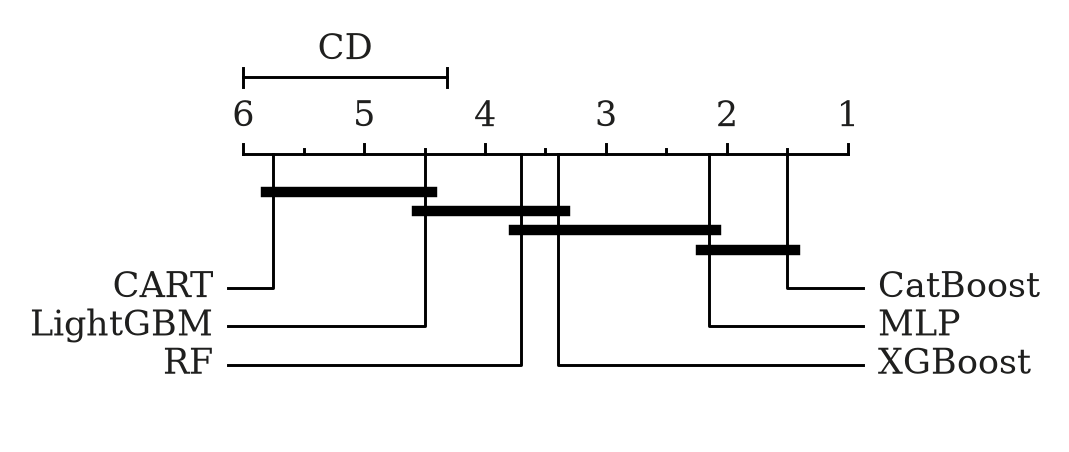
\includegraphics[width=0.90\linewidth]{cd_mrr_symmetric_label.png}\caption{MRR, symmetric}\end{subfigure}\hfill
\begin{subfigure}{0.48\linewidth}\centering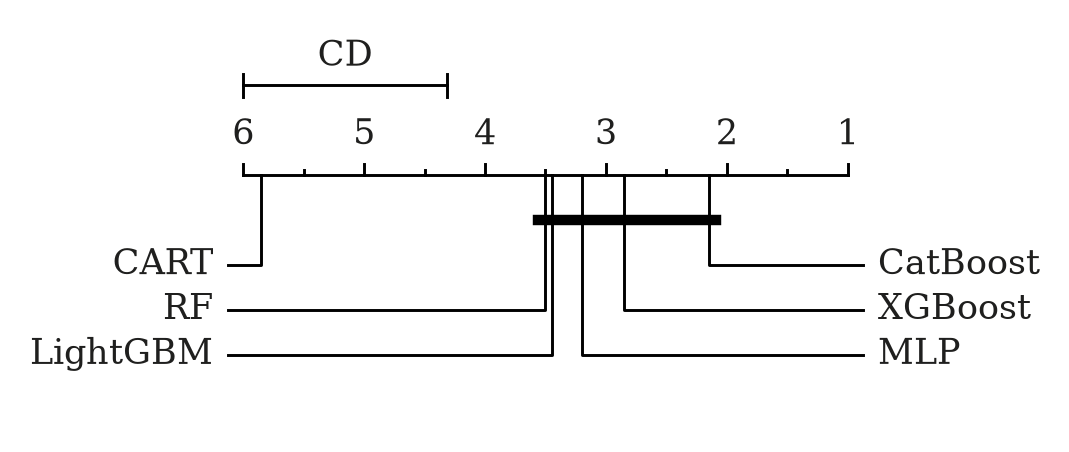
\includegraphics[width=0.90\linewidth]{cd_audc_symmetric_label.png}\caption{AUDC, symmetric}\end{subfigure}\\[1pt]
\begin{subfigure}{0.48\linewidth}\centering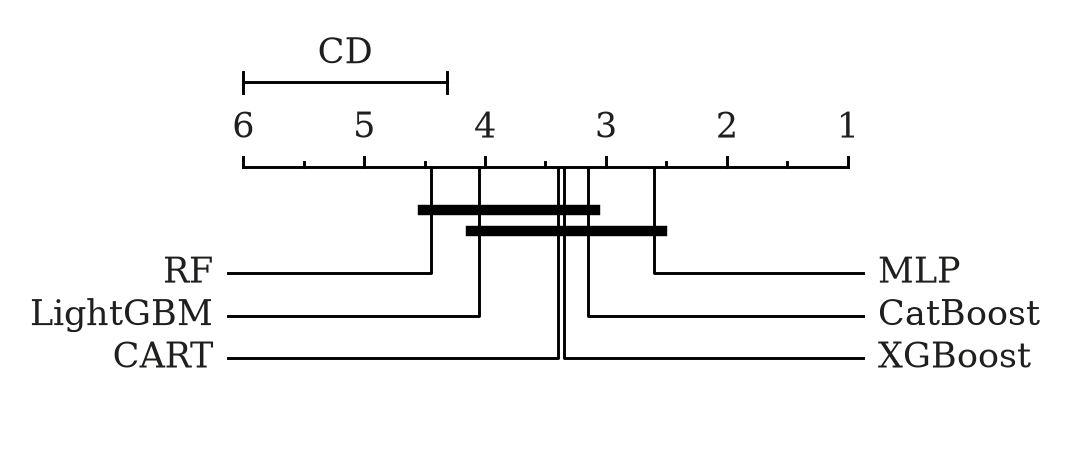
\includegraphics[width=0.90\linewidth]{cd_mrr_class_conditional.png}\caption{MRR, class-conditional}\end{subfigure}\hfill
\begin{subfigure}{0.48\linewidth}\centering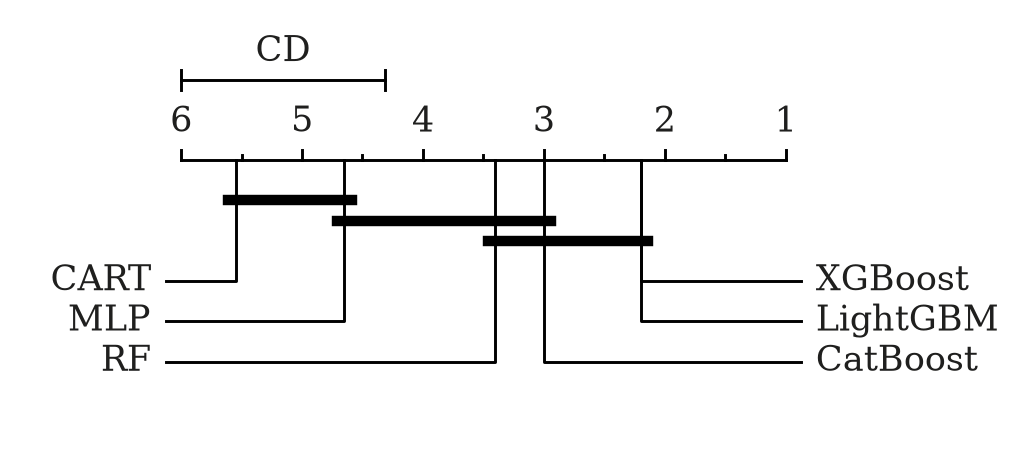
\includegraphics[width=0.90\linewidth]{cd_audc_class_conditional.png}\caption{AUDC, class-conditional}\end{subfigure}\\[1pt]
\begin{subfigure}{0.48\linewidth}\centering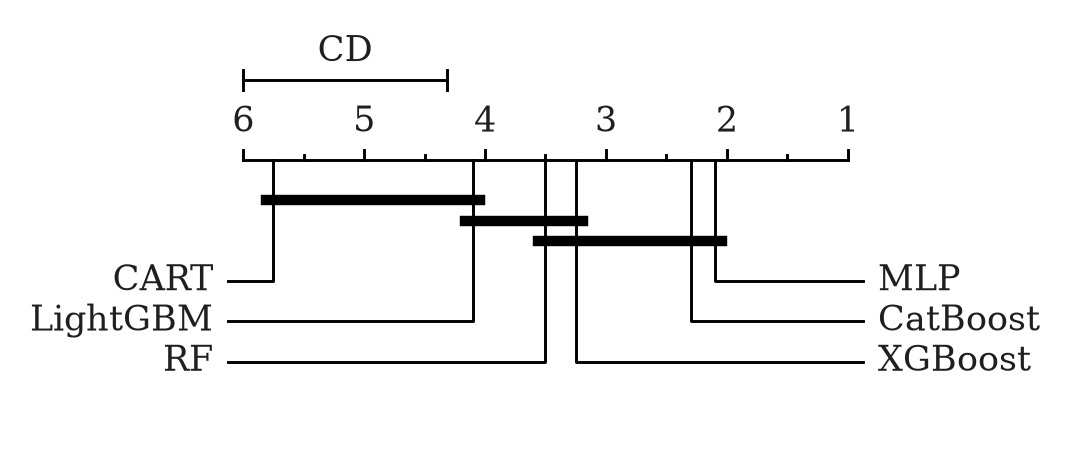
\includegraphics[width=0.90\linewidth]{cd_mrr_gaussian_feature.png}\caption{MRR, Gaussian}\end{subfigure}\hfill
\begin{subfigure}{0.48\linewidth}\centering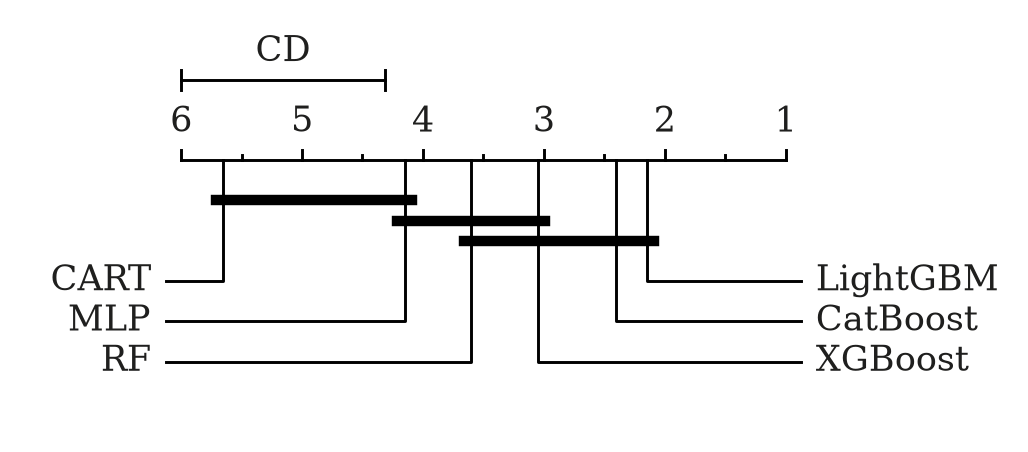
\includegraphics[width=0.90\linewidth]{cd_audc_gaussian_feature.png}\caption{AUDC, Gaussian}\end{subfigure}\\[1pt]
\begin{subfigure}{0.48\linewidth}\centering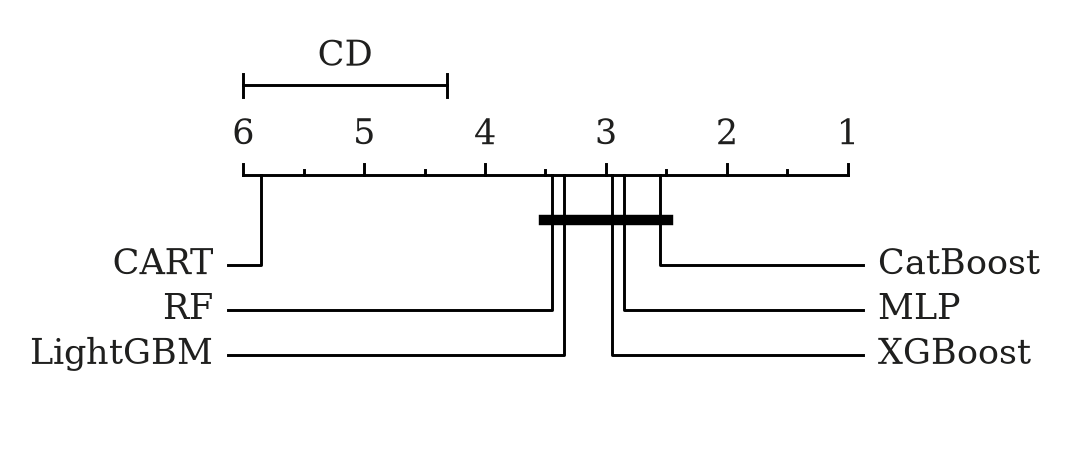
\includegraphics[width=0.90\linewidth]{cd_mrr_mcar_imputed.png}\caption{MRR, MCAR imputed}\end{subfigure}\hfill
\begin{subfigure}{0.48\linewidth}\centering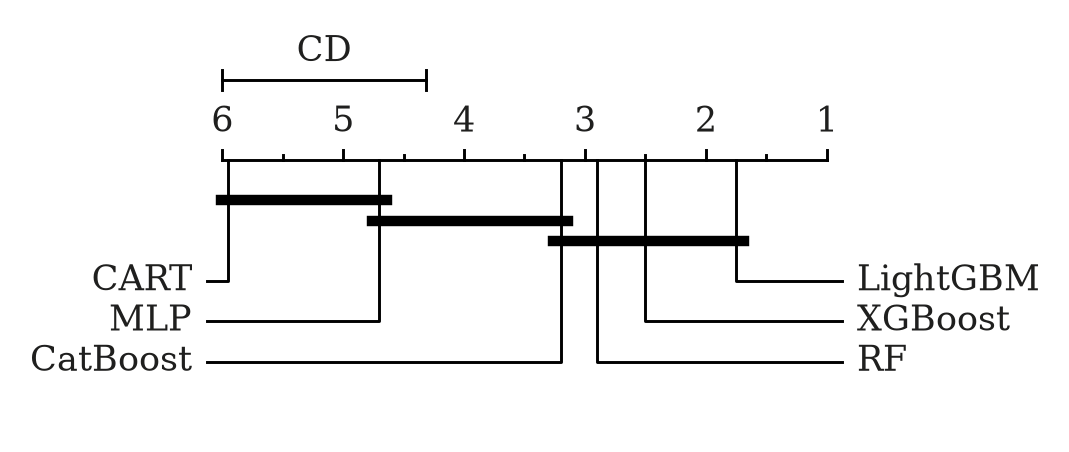
\includegraphics[width=0.90\linewidth]{cd_audc_mcar_imputed.png}\caption{AUDC, MCAR imputed}\end{subfigure}\\[1pt]
\begin{subfigure}{0.48\linewidth}\centering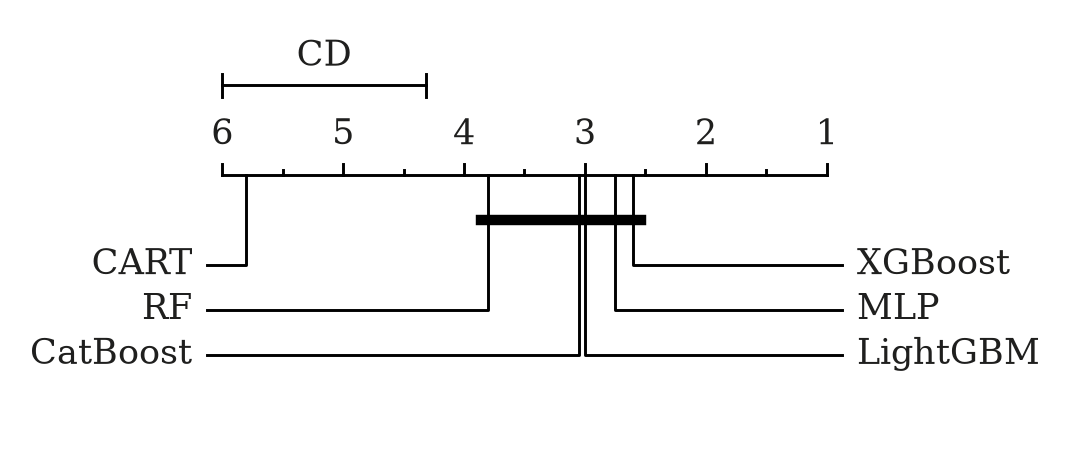
\includegraphics[width=0.90\linewidth]{cd_mrr_mcar_native.png}\caption{MRR, MCAR native}\end{subfigure}\hfill
\begin{subfigure}{0.48\linewidth}\centering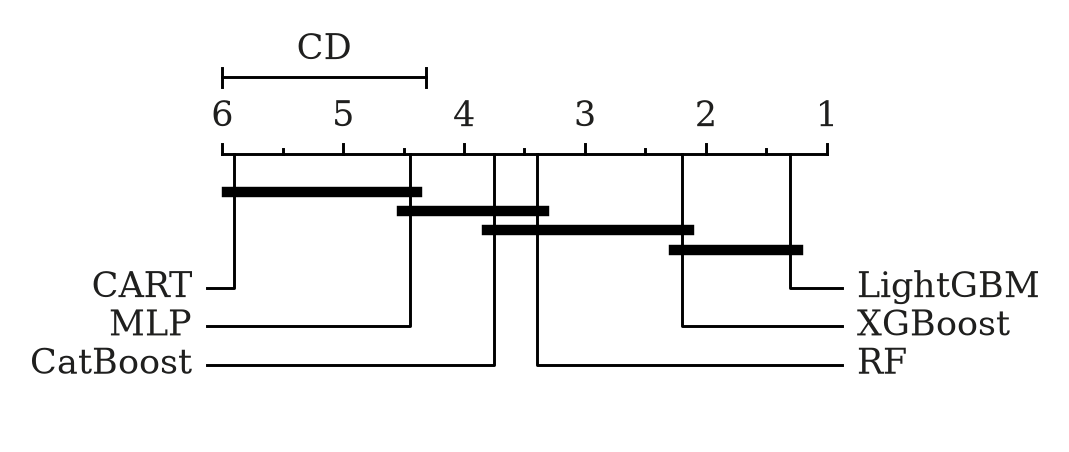
\includegraphics[width=0.90\linewidth]{cd_audc_mcar_native.png}\caption{AUDC, MCAR native}\end{subfigure}
\caption{Nemenyi critical-difference diagrams for MRR and AUDC under each primary condition (Protocol~A, seed-averaged, $N=20$, $k=6$, $\alpha=0.05$, $\mathrm{CD}=1.686$). Models joined by a bar are not significantly different.}
\label{fig:cd_all}
\end{figure}

\clearpage
\section{Per-dataset endurance}\label{sup:endurance}
%% ---- begin inlined ../results/analysis/latex_primary/tab_endurance.tex ----
\begin{table}[htbp]
\centering
\footnotesize
\setlength{\tabcolsep}{4pt}
\caption{Per-dataset MRR of the seed-averaged trajectories, averaged over the five conditions (bold = best in row). The average is descriptive only: the conditions sit on different intensity scales (Section~3.2 of the main article), and the two masking conditions share the MLP, which cannot take missing values. Per-condition values are in Supplementary Section~S5.}
\label{tab:endurance_mrr}
\begin{tabular}{@{}lrrrrrr@{}}
\toprule
Dataset & CART & RF & XGBoost & LightGBM & CatBoost & MLP \\
\midrule
\multicolumn{7}{@{}l}{\textit{Science \& sensing}} \\
Bioresponse & 89.8 & 91.6 & 92.9 & 92.9 & 93.5 & \textbf{94.1} \\
qsar-biodeg & 90.9 & 93.6 & 94.1 & 93.8 & \textbf{94.1} & 93.6 \\
eye\_movements & 81.0 & 84.5 & 86.3 & 84.2 & 89.3 & \textbf{90.4} \\
gesture\_phase & 80.8 & 86.4 & 88.1 & 85.9 & \textbf{91.8} & 90.6 \\
ozone\_level & 94.9 & 98.1 & 97.5 & 97.3 & 98.1 & \textbf{98.6} \\
\multicolumn{7}{@{}l}{\textit{Industrial \& physical}} \\
steel-plates-fault & 86.7 & 90.4 & 91.2 & 90.8 & 91.4 & \textbf{91.7} \\
vehicle & 82.8 & \textbf{92.6} & 90.0 & 88.8 & 90.6 & 88.2 \\
electricity & 86.7 & 89.8 & 90.6 & 90.2 & 93.0 & \textbf{93.6} \\
pol & 81.5 & 93.0 & 92.8 & 92.2 & \textbf{94.8} & 89.4 \\
miniboone & 91.1 & 95.1 & 94.7 & 94.7 & 95.1 & \textbf{96.0} \\
\multicolumn{7}{@{}l}{\textit{Business \& web}} \\
bank-marketing & 94.6 & 97.9 & 98.1 & 97.9 & 98.4 & \textbf{98.5} \\
churn & 91.9 & 95.5 & 95.5 & 95.1 & 95.4 & \textbf{96.0} \\
amazon\_access & 94.6 & 96.7 & 98.3 & 98.2 & 99.2 & \textbf{99.4} \\
nomao & 92.1 & 95.9 & 96.9 & 96.6 & \textbf{97.2} & 97.1 \\
spambase & 89.7 & 93.5 & 94.6 & 93.8 & \textbf{95.3} & 95.1 \\
\multicolumn{7}{@{}l}{\textit{Synthetic, game \& perceptual}} \\
madelon & 84.9 & 87.2 & 83.5 & 83.7 & 83.0 & \textbf{96.5} \\
hill\_valley & 95.5 & 92.2 & 96.1 & 91.7 & \textbf{96.8} & 96.1 \\
jungle\_chess & 80.1 & 87.8 & 89.3 & 89.3 & \textbf{90.3} & 88.2 \\
phoneme & 88.6 & 90.6 & 92.3 & 92.0 & 93.7 & \textbf{93.8} \\
volkert & 83.5 & 93.5 & 92.3 & 91.6 & \textbf{95.0} & 93.8 \\
\midrule
Mean over datasets & 88.1 & 92.3 & 92.8 & 92.0 & 93.8 & \textbf{94.0} \\
\bottomrule
\end{tabular}
\end{table}

\begin{table}[htbp]
\centering
\footnotesize
\setlength{\tabcolsep}{4pt}
\caption{Per-dataset AUDC of the seed-averaged trajectories, averaged over the five conditions (bold = best in row). The average is descriptive only: the conditions sit on different intensity scales (Section~3.2 of the main article), and the two masking conditions share the MLP, which cannot take missing values. Per-condition values are in Supplementary Section~S5.}
\label{tab:endurance_audc}
\begin{tabular}{@{}lrrrrrr@{}}
\toprule
Dataset & CART & RF & XGBoost & LightGBM & CatBoost & MLP \\
\midrule
\multicolumn{7}{@{}l}{\textit{Science \& sensing}} \\
Bioresponse & 65.2 & 73.3 & \textbf{74.5} & 74.4 & 73.8 & 73.0 \\
qsar-biodeg & 74.1 & 81.7 & 81.4 & 81.3 & \textbf{82.1} & 82.0 \\
eye\_movements & 47.1 & 57.7 & 58.7 & \textbf{59.4} & 55.8 & 51.6 \\
gesture\_phase & 41.0 & \textbf{57.5} & 56.3 & 57.2 & 53.0 & 51.3 \\
ozone\_level & 86.4 & 92.5 & 92.0 & 91.9 & 92.6 & \textbf{92.9} \\
\multicolumn{7}{@{}l}{\textit{Industrial \& physical}} \\
steel-plates-fault & 86.7 & 89.8 & 91.2 & 90.8 & \textbf{91.4} & 91.1 \\
vehicle & 57.8 & \textbf{69.1} & 68.2 & 68.3 & 68.5 & 65.7 \\
electricity & 70.1 & 76.7 & 77.2 & \textbf{77.5} & 76.1 & 74.1 \\
pol & 70.0 & 80.5 & 81.1 & 81.1 & 79.8 & \textbf{82.4} \\
miniboone & 79.8 & 87.9 & 88.6 & 88.7 & \textbf{88.9} & 87.0 \\
\multicolumn{7}{@{}l}{\textit{Business \& web}} \\
bank-marketing & 81.9 & 88.1 & 88.5 & 88.3 & \textbf{89.0} & 88.5 \\
churn & 84.1 & 90.8 & 90.8 & 90.6 & \textbf{91.2} & 89.4 \\
amazon\_access & 86.2 & 91.4 & 92.9 & 92.8 & 93.5 & \textbf{93.7} \\
nomao & 85.7 & 91.8 & 92.7 & 92.8 & \textbf{93.0} & 92.3 \\
spambase & 81.6 & 89.2 & 90.2 & 89.8 & \textbf{90.7} & 89.5 \\
\multicolumn{7}{@{}l}{\textit{Synthetic, game \& perceptual}} \\
madelon & 62.6 & 61.7 & 69.4 & 69.0 & \textbf{69.9} & 53.9 \\
hill\_valley & 51.7 & 52.8 & 52.0 & \textbf{53.1} & 51.3 & 51.5 \\
jungle\_chess & 63.4 & 71.5 & 75.6 & \textbf{76.0} & 76.0 & 74.6 \\
phoneme & 77.0 & \textbf{82.4} & 82.4 & 82.4 & 82.1 & 80.5 \\
volkert & 38.3 & 55.8 & 57.3 & \textbf{57.4} & 55.6 & 54.8 \\
\midrule
Mean over datasets & 69.5 & 77.1 & 78.0 & \textbf{78.1} & 77.7 & 76.0 \\
\bottomrule
\end{tabular}
\end{table}
%% ---- end inlined ../results/analysis/latex_primary/tab_endurance.tex ----

\clearpage
\section{Trajectory summaries for every dataset}\label{sup:traj}
For every dataset, model and primary condition, the tables give clean and terminal accuracy, AUDC, MRR and $\etaknee$ with its 95\% parametric-bootstrap interval, on seed-averaged trajectories. The interval is printed because the knee of a single trajectory is not reliable on its own (Section~5.6 of the main article).
%% ---- begin inlined ../results/analysis/latex_primary/tab_trajectories.tex ----
\begin{table}[htbp]
\centering
\scriptsize
\setlength{\tabcolsep}{3.5pt}
\caption{Trajectory summaries for \texttt{Bioresponse}, accuracy averaged over seeds 42, 43 and 44. $\eta_{\mathrm{knee}}$ and its 95\% parametric-bootstrap interval ($B=200$; the standard error of each tier is $\max(\mathrm{SD}_{\mathrm{seed}},\,\mathrm{SD}_{\mathrm{fold}}/2)/\sqrt3$); ``flat'' marks a trajectory with $\kappa\equiv 0$, for which $\eta_{\mathrm{knee}}$ is undefined. Values are rounded to the nearest of the eleven experimental tiers (spacing $0.05$); the knee is a coarse, secondary population-level descriptor.}
\label{tab:traj_Bioresponse}
\begin{tabular}{@{}llrrrrl@{}}
\toprule
Condition & Model & $\mathrm{Acc}(0)$ & $\mathrm{Acc}(0.5)$ & AUDC & MRR & $\eta_{\mathrm{knee}}$ [95\% CI] \\
\midrule
Symmetric label & CART & 0.726 & 0.498 & 0.609 & 0.839 & 0.25 [0.05, 0.45] \\
 & RF & 0.801 & 0.496 & 0.687 & 0.858 & 0.25 [0.05, 0.40] \\
 & XGBoost & 0.801 & 0.501 & 0.697 & 0.870 & 0.35 [0.05, 0.40] \\
 & LightGBM & 0.800 & 0.493 & 0.691 & 0.863 & 0.05 [0.05, 0.40] \\
 & CatBoost & 0.789 & 0.497 & 0.715 & 0.906 & 0.25 [0.05, 0.35] \\
 & MLP & 0.776 & 0.491 & 0.676 & 0.871 & 0.25 [0.05, 0.40] \\
\midrule
Class-cond.\ label & CART & 0.726 & 0.635 & 0.680 & 0.936 & 0.20 [0.05, 0.45] \\
 & RF & 0.801 & 0.606 & 0.720 & 0.899 & 0.15 [0.05, 0.45] \\
 & XGBoost & 0.801 & 0.622 & 0.734 & 0.916 & 0.05 [0.05, 0.45] \\
 & LightGBM & 0.800 & 0.630 & 0.734 & 0.917 & 0.15 [0.05, 0.45] \\
 & CatBoost & 0.789 & 0.581 & 0.717 & 0.908 & 0.25 [0.05, 0.45] \\
 & MLP & 0.776 & 0.582 & 0.713 & 0.919 & 0.45 [0.10, 0.45] \\
\midrule
Gaussian feature & CART & 0.726 & 0.637 & 0.651 & 0.897 & 0.05 [0.05, 0.45] \\
 & RF & 0.801 & 0.734 & 0.750 & 0.936 & 0.05 [0.05, 0.30] \\
 & XGBoost & 0.801 & 0.758 & 0.768 & 0.958 & 0.05 [0.05, 0.45] \\
 & LightGBM & 0.800 & 0.759 & 0.769 & 0.960 & 0.05 [0.05, 0.45] \\
 & CatBoost & 0.789 & 0.749 & 0.757 & 0.959 & 0.05 [0.05, 0.45] \\
 & MLP & 0.776 & 0.742 & 0.762 & 0.982 & 0.40 [0.05, 0.45] \\
\midrule
MCAR, imputed & CART & 0.726 & 0.615 & 0.666 & 0.918 & 0.35 [0.05, 0.45] \\
 & RF & 0.801 & 0.724 & 0.766 & 0.956 & 0.10 [0.05, 0.45] \\
 & XGBoost & 0.801 & 0.728 & 0.766 & 0.956 & 0.25 [0.05, 0.45] \\
 & LightGBM & 0.800 & 0.734 & 0.768 & 0.960 & 0.20 [0.10, 0.45] \\
 & CatBoost & 0.789 & 0.723 & 0.756 & 0.957 & 0.25 [0.05, 0.45] \\
 & MLP & 0.776 & 0.717 & 0.749 & 0.965 & 0.15 [0.05, 0.45] \\
\midrule
MCAR, native & CART & 0.726 & 0.617 & 0.652 & 0.898 & 0.40 [0.05, 0.45] \\
 & RF & 0.801 & 0.700 & 0.743 & 0.928 & 0.40 [0.05, 0.40] \\
 & XGBoost & 0.801 & 0.725 & 0.758 & 0.946 & 0.05 [0.05, 0.45] \\
 & LightGBM & 0.800 & 0.729 & 0.758 & 0.947 & 0.25 [0.05, 0.45] \\
 & CatBoost & 0.789 & 0.717 & 0.747 & 0.946 & 0.05 [0.05, 0.45] \\
 & MLP & 0.776 & 0.717 & 0.749 & 0.965 & 0.15 [0.05, 0.45] \\
\bottomrule
\end{tabular}
\end{table}

\begin{table}[htbp]
\centering
\scriptsize
\setlength{\tabcolsep}{3.5pt}
\caption{Trajectory summaries for \texttt{qsar-biodeg}, accuracy averaged over seeds 42, 43 and 44. $\eta_{\mathrm{knee}}$ and its 95\% parametric-bootstrap interval ($B=200$; the standard error of each tier is $\max(\mathrm{SD}_{\mathrm{seed}},\,\mathrm{SD}_{\mathrm{fold}}/2)/\sqrt3$); ``flat'' marks a trajectory with $\kappa\equiv 0$, for which $\eta_{\mathrm{knee}}$ is undefined. Values are rounded to the nearest of the eleven experimental tiers (spacing $0.05$); the knee is a coarse, secondary population-level descriptor.}
\label{tab:traj_qsar_biodeg}
\begin{tabular}{@{}llrrrrl@{}}
\toprule
Condition & Model & $\mathrm{Acc}(0)$ & $\mathrm{Acc}(0.5)$ & AUDC & MRR & $\eta_{\mathrm{knee}}$ [95\% CI] \\
\midrule
Symmetric label & CART & 0.815 & 0.494 & 0.654 & 0.802 & 0.45 [0.15, 0.45] \\
 & RF & 0.873 & 0.517 & 0.746 & 0.854 & 0.15 [0.05, 0.45] \\
 & XGBoost & 0.866 & 0.486 & 0.726 & 0.839 & 0.15 [0.05, 0.45] \\
 & LightGBM & 0.867 & 0.493 & 0.718 & 0.829 & 0.15 [0.05, 0.45] \\
 & CatBoost & 0.872 & 0.497 & 0.755 & 0.865 & 0.25 [0.05, 0.40] \\
 & MLP & 0.876 & 0.551 & 0.781 & 0.892 & 0.20 [0.10, 0.45] \\
\midrule
Class-cond.\ label & CART & 0.815 & 0.737 & 0.771 & 0.947 & 0.35 [0.05, 0.40] \\
 & RF & 0.873 & 0.734 & 0.810 & 0.928 & 0.30 [0.10, 0.45] \\
 & XGBoost & 0.866 & 0.747 & 0.817 & 0.943 & 0.15 [0.05, 0.45] \\
 & LightGBM & 0.867 & 0.743 & 0.814 & 0.939 & 0.10 [0.10, 0.45] \\
 & CatBoost & 0.872 & 0.737 & 0.818 & 0.938 & 0.15 [0.05, 0.45] \\
 & MLP & 0.876 & 0.682 & 0.801 & 0.914 & 0.30 [0.15, 0.45] \\
\midrule
Gaussian feature & CART & 0.815 & 0.720 & 0.760 & 0.933 & 0.20 [0.05, 0.45] \\
 & RF & 0.873 & 0.822 & 0.845 & 0.968 & 0.05 [0.05, 0.45] \\
 & XGBoost & 0.866 & 0.829 & 0.844 & 0.975 & 0.10 [0.05, 0.45] \\
 & LightGBM & 0.867 & 0.824 & 0.845 & 0.975 & 0.20 [0.05, 0.45] \\
 & CatBoost & 0.872 & 0.824 & 0.845 & 0.969 & 0.35 [0.10, 0.45] \\
 & MLP & 0.876 & 0.819 & 0.848 & 0.968 & 0.10 [0.05, 0.45] \\
\midrule
MCAR, imputed & CART & 0.815 & 0.713 & 0.765 & 0.939 & 0.40 [0.15, 0.45] \\
 & RF & 0.873 & 0.810 & 0.845 & 0.967 & 0.35 [0.05, 0.45] \\
 & XGBoost & 0.866 & 0.817 & 0.844 & 0.975 & 0.05 [0.05, 0.45] \\
 & LightGBM & 0.867 & 0.815 & 0.844 & 0.974 & 0.05 [0.05, 0.45] \\
 & CatBoost & 0.872 & 0.810 & 0.847 & 0.971 & 0.35 [0.05, 0.45] \\
 & MLP & 0.876 & 0.801 & 0.835 & 0.953 & 0.05 [0.05, 0.45] \\
\midrule
MCAR, native & CART & 0.815 & 0.714 & 0.755 & 0.926 & 0.30 [0.10, 0.45] \\
 & RF & 0.873 & 0.797 & 0.839 & 0.961 & 0.25 [0.05, 0.45] \\
 & XGBoost & 0.866 & 0.811 & 0.841 & 0.971 & 0.30 [0.05, 0.45] \\
 & LightGBM & 0.867 & 0.809 & 0.842 & 0.972 & 0.05 [0.05, 0.45] \\
 & CatBoost & 0.872 & 0.803 & 0.839 & 0.962 & 0.40 [0.05, 0.40] \\
 & MLP & 0.876 & 0.801 & 0.835 & 0.953 & 0.05 [0.05, 0.45] \\
\bottomrule
\end{tabular}
\end{table}

\begin{table}[htbp]
\centering
\scriptsize
\setlength{\tabcolsep}{3.5pt}
\caption{Trajectory summaries for \texttt{eye\_movements}, accuracy averaged over seeds 42, 43 and 44. $\eta_{\mathrm{knee}}$ and its 95\% parametric-bootstrap interval ($B=200$; the standard error of each tier is $\max(\mathrm{SD}_{\mathrm{seed}},\,\mathrm{SD}_{\mathrm{fold}}/2)/\sqrt3$); ``flat'' marks a trajectory with $\kappa\equiv 0$, for which $\eta_{\mathrm{knee}}$ is undefined. Values are rounded to the nearest of the eleven experimental tiers (spacing $0.05$); the knee is a coarse, secondary population-level descriptor.}
\label{tab:traj_eye_movements}
\begin{tabular}{@{}llrrrrl@{}}
\toprule
Condition & Model & $\mathrm{Acc}(0)$ & $\mathrm{Acc}(0.5)$ & AUDC & MRR & $\eta_{\mathrm{knee}}$ [95\% CI] \\
\midrule
Symmetric label & CART & 0.581 & 0.371 & 0.464 & 0.798 & 0.05 [0.05, 0.45] \\
 & RF & 0.683 & 0.472 & 0.595 & 0.871 & 0.40 [0.05, 0.45] \\
 & XGBoost & 0.680 & 0.482 & 0.600 & 0.883 & 0.15 [0.10, 0.35] \\
 & LightGBM & 0.705 & 0.470 & 0.607 & 0.861 & 0.15 [0.10, 0.45] \\
 & CatBoost & 0.625 & 0.502 & 0.577 & 0.924 & 0.40 [0.10, 0.45] \\
 & MLP & 0.570 & 0.444 & 0.519 & 0.910 & 0.10 [0.05, 0.45] \\
\midrule
Class-cond.\ label & CART & 0.581 & 0.378 & 0.468 & 0.805 & 0.15 [0.05, 0.40] \\
 & RF & 0.683 & 0.446 & 0.587 & 0.860 & 0.20 [0.05, 0.45] \\
 & XGBoost & 0.680 & 0.443 & 0.589 & 0.866 & 0.15 [0.05, 0.45] \\
 & LightGBM & 0.705 & 0.441 & 0.596 & 0.845 & 0.15 [0.05, 0.45] \\
 & CatBoost & 0.625 & 0.453 & 0.560 & 0.897 & 0.15 [0.05, 0.45] \\
 & MLP & 0.570 & 0.432 & 0.513 & 0.901 & 0.10 [0.05, 0.45] \\
\midrule
Gaussian feature & CART & 0.581 & 0.425 & 0.477 & 0.821 & 0.05 [0.05, 0.45] \\
 & RF & 0.683 & 0.509 & 0.574 & 0.841 & 0.05 [0.05, 0.45] \\
 & XGBoost & 0.680 & 0.516 & 0.582 & 0.856 & 0.05 [0.05, 0.45] \\
 & LightGBM & 0.705 & 0.515 & 0.587 & 0.833 & 0.05 [0.05, 0.45] \\
 & CatBoost & 0.625 & 0.512 & 0.560 & 0.897 & 0.05 [0.05, 0.45] \\
 & MLP & 0.570 & 0.503 & 0.536 & 0.940 & 0.10 [0.05, 0.45] \\
\midrule
MCAR, imputed & CART & 0.581 & 0.420 & 0.478 & 0.823 & 0.35 [0.05, 0.45] \\
 & RF & 0.683 & 0.494 & 0.568 & 0.832 & 0.15 [0.05, 0.45] \\
 & XGBoost & 0.680 & 0.508 & 0.580 & 0.853 & 0.10 [0.05, 0.45] \\
 & LightGBM & 0.705 & 0.507 & 0.589 & 0.835 & 0.25 [0.05, 0.45] \\
 & CatBoost & 0.625 & 0.493 & 0.551 & 0.883 & 0.10 [0.05, 0.45] \\
 & MLP & 0.570 & 0.461 & 0.505 & 0.886 & 0.40 [0.05, 0.45] \\
\midrule
MCAR, native & CART & 0.581 & 0.413 & 0.468 & 0.805 & 0.20 [0.05, 0.45] \\
 & RF & 0.683 & 0.484 & 0.560 & 0.821 & 0.10 [0.05, 0.45] \\
 & XGBoost & 0.680 & 0.510 & 0.583 & 0.858 & 0.10 [0.05, 0.40] \\
 & LightGBM & 0.705 & 0.506 & 0.591 & 0.838 & 0.45 [0.10, 0.45] \\
 & CatBoost & 0.625 & 0.479 & 0.539 & 0.863 & 0.25 [0.05, 0.45] \\
 & MLP & 0.570 & 0.461 & 0.505 & 0.886 & 0.40 [0.05, 0.45] \\
\bottomrule
\end{tabular}
\end{table}

\begin{table}[htbp]
\centering
\scriptsize
\setlength{\tabcolsep}{3.5pt}
\caption{Trajectory summaries for \texttt{gesture\_phase}, accuracy averaged over seeds 42, 43 and 44. $\eta_{\mathrm{knee}}$ and its 95\% parametric-bootstrap interval ($B=200$; the standard error of each tier is $\max(\mathrm{SD}_{\mathrm{seed}},\,\mathrm{SD}_{\mathrm{fold}}/2)/\sqrt3$); ``flat'' marks a trajectory with $\kappa\equiv 0$, for which $\eta_{\mathrm{knee}}$ is undefined. Values are rounded to the nearest of the eleven experimental tiers (spacing $0.05$); the knee is a coarse, secondary population-level descriptor.}
\label{tab:traj_gesture_phase}
\begin{tabular}{@{}llrrrrl@{}}
\toprule
Condition & Model & $\mathrm{Acc}(0)$ & $\mathrm{Acc}(0.5)$ & AUDC & MRR & $\eta_{\mathrm{knee}}$ [95\% CI] \\
\midrule
Symmetric label & CART & 0.507 & 0.307 & 0.407 & 0.802 & 0.35 [0.10, 0.45] \\
 & RF & 0.666 & 0.544 & 0.627 & 0.942 & 0.25 [0.05, 0.45] \\
 & XGBoost & 0.639 & 0.520 & 0.597 & 0.934 & 0.30 [0.05, 0.40] \\
 & LightGBM & 0.666 & 0.509 & 0.605 & 0.909 & 0.35 [0.05, 0.45] \\
 & CatBoost & 0.578 & 0.530 & 0.559 & 0.968 & 0.45 [0.05, 0.45] \\
 & MLP & 0.567 & 0.475 & 0.525 & 0.926 & 0.10 [0.05, 0.40] \\
\midrule
Class-cond.\ label & CART & 0.507 & 0.314 & 0.408 & 0.804 & 0.15 [0.05, 0.45] \\
 & RF & 0.666 & 0.386 & 0.587 & 0.882 & 0.30 [0.05, 0.35] \\
 & XGBoost & 0.639 & 0.368 & 0.557 & 0.871 & 0.30 [0.05, 0.35] \\
 & LightGBM & 0.666 & 0.372 & 0.564 & 0.847 & 0.30 [0.05, 0.40] \\
 & CatBoost & 0.578 & 0.352 & 0.531 & 0.919 & 0.40 [0.05, 0.40] \\
 & MLP & 0.567 & 0.319 & 0.495 & 0.873 & 0.40 [0.05, 0.45] \\
\midrule
Gaussian feature & CART & 0.507 & 0.348 & 0.393 & 0.775 & 0.05 [0.05, 0.45] \\
 & RF & 0.666 & 0.481 & 0.539 & 0.810 & 0.05 [0.05, 0.45] \\
 & XGBoost & 0.639 & 0.485 & 0.537 & 0.841 & 0.05 [0.05, 0.45] \\
 & LightGBM & 0.666 & 0.483 & 0.539 & 0.810 & 0.05 [0.05, 0.40] \\
 & CatBoost & 0.578 & 0.481 & 0.520 & 0.901 & 0.10 [0.05, 0.45] \\
 & MLP & 0.567 & 0.479 & 0.519 & 0.916 & 0.25 [0.05, 0.45] \\
\midrule
MCAR, imputed & CART & 0.507 & 0.378 & 0.426 & 0.840 & 0.10 [0.10, 0.45] \\
 & RF & 0.666 & 0.500 & 0.567 & 0.851 & 0.30 [0.05, 0.40] \\
 & XGBoost & 0.639 & 0.506 & 0.563 & 0.881 & 0.25 [0.15, 0.45] \\
 & LightGBM & 0.666 & 0.513 & 0.579 & 0.870 & 0.30 [0.10, 0.45] \\
 & CatBoost & 0.578 & 0.491 & 0.528 & 0.915 & 0.35 [0.05, 0.45] \\
 & MLP & 0.567 & 0.475 & 0.514 & 0.907 & 0.10 [0.05, 0.45] \\
\midrule
MCAR, native & CART & 0.507 & 0.366 & 0.415 & 0.818 & 0.20 [0.05, 0.45] \\
 & RF & 0.666 & 0.493 & 0.555 & 0.833 & 0.40 [0.10, 0.45] \\
 & XGBoost & 0.639 & 0.504 & 0.560 & 0.877 & 0.35 [0.05, 0.45] \\
 & LightGBM & 0.666 & 0.506 & 0.572 & 0.859 & 0.35 [0.05, 0.45] \\
 & CatBoost & 0.578 & 0.468 & 0.511 & 0.886 & 0.15 [0.05, 0.40] \\
 & MLP & 0.567 & 0.475 & 0.514 & 0.907 & 0.10 [0.05, 0.45] \\
\bottomrule
\end{tabular}
\end{table}

\begin{table}[htbp]
\centering
\scriptsize
\setlength{\tabcolsep}{3.5pt}
\caption{Trajectory summaries for \texttt{ozone\_level}, accuracy averaged over seeds 42, 43 and 44. $\eta_{\mathrm{knee}}$ and its 95\% parametric-bootstrap interval ($B=200$; the standard error of each tier is $\max(\mathrm{SD}_{\mathrm{seed}},\,\mathrm{SD}_{\mathrm{fold}}/2)/\sqrt3$); ``flat'' marks a trajectory with $\kappa\equiv 0$, for which $\eta_{\mathrm{knee}}$ is undefined. Values are rounded to the nearest of the eleven experimental tiers (spacing $0.05$); the knee is a coarse, secondary population-level descriptor.}
\label{tab:traj_ozone_level}
\begin{tabular}{@{}llrrrrl@{}}
\toprule
Condition & Model & $\mathrm{Acc}(0)$ & $\mathrm{Acc}(0.5)$ & AUDC & MRR & $\eta_{\mathrm{knee}}$ [95\% CI] \\
\midrule
Symmetric label & CART & 0.910 & 0.499 & 0.694 & 0.762 & 0.30 [0.05, 0.45] \\
 & RF & 0.943 & 0.518 & 0.867 & 0.919 & 0.35 [0.20, 0.35] \\
 & XGBoost & 0.944 & 0.499 & 0.838 & 0.888 & 0.20 [0.10, 0.35] \\
 & LightGBM & 0.944 & 0.495 & 0.827 & 0.876 & 0.20 [0.10, 0.35] \\
 & CatBoost & 0.943 & 0.486 & 0.867 & 0.919 & 0.35 [0.20, 0.35] \\
 & MLP & 0.942 & 0.513 & 0.887 & 0.942 & 0.35 [0.25, 0.40] \\
\midrule
Class-cond.\ label & CART & 0.910 & 0.922 & 0.916 & 1.006 & 0.30 [0.05, 0.40] \\
 & RF & 0.943 & 0.938 & 0.940 & 0.997 & 0.10 [0.05, 0.40] \\
 & XGBoost & 0.944 & 0.939 & 0.941 & 0.997 & 0.25 [0.05, 0.45] \\
 & LightGBM & 0.944 & 0.939 & 0.942 & 0.998 & 0.15 [0.05, 0.45] \\
 & CatBoost & 0.943 & 0.938 & 0.940 & 0.997 & 0.05 [0.05, 0.40] \\
 & MLP & 0.942 & 0.937 & 0.939 & 0.997 & 0.25 [0.05, 0.35] \\
\midrule
Gaussian feature & CART & 0.910 & 0.898 & 0.905 & 0.994 & 0.20 [0.05, 0.45] \\
 & RF & 0.943 & 0.938 & 0.940 & 0.997 & 0.35 [0.05, 0.40] \\
 & XGBoost & 0.944 & 0.940 & 0.942 & 0.998 & 0.30 [0.05, 0.45] \\
 & LightGBM & 0.944 & 0.937 & 0.942 & 0.999 & 0.45 [0.05, 0.45] \\
 & CatBoost & 0.943 & 0.939 & 0.942 & 0.999 & 0.20 [0.05, 0.45] \\
 & MLP & 0.942 & 0.938 & 0.940 & 0.998 & 0.35 [0.10, 0.45] \\
\midrule
MCAR, imputed & CART & 0.910 & 0.896 & 0.903 & 0.992 & 0.10 [0.10, 0.40] \\
 & RF & 0.943 & 0.938 & 0.939 & 0.996 & 0.10 [0.05, 0.40] \\
 & XGBoost & 0.944 & 0.937 & 0.940 & 0.996 & 0.25 [0.05, 0.40] \\
 & LightGBM & 0.944 & 0.940 & 0.941 & 0.997 & 0.35 [0.05, 0.45] \\
 & CatBoost & 0.943 & 0.938 & 0.940 & 0.996 & 0.30 [0.05, 0.40] \\
 & MLP & 0.942 & 0.936 & 0.939 & 0.997 & 0.05 [0.05, 0.45] \\
\midrule
MCAR, native & CART & 0.910 & 0.896 & 0.903 & 0.991 & 0.35 [0.05, 0.45] \\
 & RF & 0.943 & 0.937 & 0.939 & 0.996 & 0.10 [0.05, 0.40] \\
 & XGBoost & 0.944 & 0.939 & 0.940 & 0.996 & 0.15 [0.05, 0.45] \\
 & LightGBM & 0.944 & 0.939 & 0.940 & 0.996 & 0.10 [0.05, 0.45] \\
 & CatBoost & 0.943 & 0.937 & 0.939 & 0.996 & 0.45 [0.05, 0.45] \\
 & MLP & 0.942 & 0.936 & 0.939 & 0.997 & 0.05 [0.05, 0.45] \\
\bottomrule
\end{tabular}
\end{table}

\begin{table}[htbp]
\centering
\scriptsize
\setlength{\tabcolsep}{3.5pt}
\caption{Trajectory summaries for \texttt{steel-plates-fault}, accuracy averaged over seeds 42, 43 and 44. $\eta_{\mathrm{knee}}$ and its 95\% parametric-bootstrap interval ($B=200$; the standard error of each tier is $\max(\mathrm{SD}_{\mathrm{seed}},\,\mathrm{SD}_{\mathrm{fold}}/2)/\sqrt3$); ``flat'' marks a trajectory with $\kappa\equiv 0$, for which $\eta_{\mathrm{knee}}$ is undefined. Values are rounded to the nearest of the eleven experimental tiers (spacing $0.05$); the knee is a coarse, secondary population-level descriptor.}
\label{tab:traj_steel_plates_fault}
\begin{tabular}{@{}llrrrrl@{}}
\toprule
Condition & Model & $\mathrm{Acc}(0)$ & $\mathrm{Acc}(0.5)$ & AUDC & MRR & $\eta_{\mathrm{knee}}$ [95\% CI] \\
\midrule
Symmetric label & CART & 1.000 & 0.507 & 0.727 & 0.727 & 0.45 [0.10, 0.45] \\
 & RF & 0.993 & 0.503 & 0.824 & 0.830 & 0.15 [0.10, 0.45] \\
 & XGBoost & 1.000 & 0.507 & 0.836 & 0.836 & 0.20 [0.10, 0.50] \\
 & LightGBM & 1.000 & 0.506 & 0.824 & 0.824 & 0.15 [0.10, 0.45] \\
 & CatBoost & 1.000 & 0.493 & 0.858 & 0.858 & 0.15 [0.15, 0.45] \\
 & MLP & 0.993 & 0.513 & 0.902 & 0.907 & 0.30 [0.20, 0.50] \\
\midrule
Class-cond.\ label & CART & 1.000 & 0.828 & 0.907 & 0.907 & 0.40 [0.10, 0.45] \\
 & RF & 0.993 & 0.733 & 0.898 & 0.904 & 0.15 [0.10, 0.45] \\
 & XGBoost & 1.000 & 0.802 & 0.941 & 0.941 & 0.25 [0.15, 0.45] \\
 & LightGBM & 1.000 & 0.806 & 0.933 & 0.933 & 0.25 [0.10, 0.45] \\
 & CatBoost & 1.000 & 0.766 & 0.935 & 0.935 & 0.25 [0.15, 0.45] \\
 & MLP & 0.993 & 0.713 & 0.932 & 0.938 & 0.30 [0.15, 0.45] \\
\midrule
Gaussian feature & CART & 1.000 & 0.986 & 0.996 & 0.996 & 0.45 [0.05, 0.45] \\
 & RF & 0.993 & 0.990 & 0.993 & 1.000 & 0.40 [0.05, 0.45] \\
 & XGBoost & 1.000 & 0.991 & 0.994 & 0.994 & 0.05 [0.05, 0.40] \\
 & LightGBM & 1.000 & 0.991 & 0.995 & 0.995 & 0.05 [0.05, 0.45] \\
 & CatBoost & 1.000 & 0.992 & 0.996 & 0.996 & 0.05 [0.05, 0.45] \\
 & MLP & 0.993 & 0.964 & 0.986 & 0.992 & 0.35 [0.10, 0.45] \\
\midrule
MCAR, imputed & CART & 1.000 & 0.742 & 0.843 & 0.843 & 0.25 [0.05, 0.45] \\
 & RF & 0.993 & 0.780 & 0.880 & 0.886 & 0.20 [0.10, 0.45] \\
 & XGBoost & 1.000 & 0.782 & 0.884 & 0.884 & 0.20 [0.10, 0.45] \\
 & LightGBM & 1.000 & 0.776 & 0.882 & 0.882 & 0.40 [0.10, 0.45] \\
 & CatBoost & 1.000 & 0.780 & 0.884 & 0.884 & 0.15 [0.10, 0.45] \\
 & MLP & 0.993 & 0.758 & 0.869 & 0.875 & 0.30 [0.10, 0.45] \\
\midrule
MCAR, native & CART & 1.000 & 0.742 & 0.863 & 0.863 & 0.35 [0.10, 0.45] \\
 & RF & 0.993 & 0.791 & 0.893 & 0.899 & 0.20 [0.10, 0.45] \\
 & XGBoost & 1.000 & 0.806 & 0.903 & 0.903 & 0.10 [0.10, 0.45] \\
 & LightGBM & 1.000 & 0.803 & 0.904 & 0.904 & 0.30 [0.05, 0.45] \\
 & CatBoost & 1.000 & 0.786 & 0.894 & 0.894 & 0.10 [0.10, 0.45] \\
 & MLP & 0.993 & 0.758 & 0.869 & 0.875 & 0.30 [0.15, 0.45] \\
\bottomrule
\end{tabular}
\end{table}

\begin{table}[htbp]
\centering
\scriptsize
\setlength{\tabcolsep}{3.5pt}
\caption{Trajectory summaries for \texttt{vehicle}, accuracy averaged over seeds 42, 43 and 44. $\eta_{\mathrm{knee}}$ and its 95\% parametric-bootstrap interval ($B=200$; the standard error of each tier is $\max(\mathrm{SD}_{\mathrm{seed}},\,\mathrm{SD}_{\mathrm{fold}}/2)/\sqrt3$); ``flat'' marks a trajectory with $\kappa\equiv 0$, for which $\eta_{\mathrm{knee}}$ is undefined. Values are rounded to the nearest of the eleven experimental tiers (spacing $0.05$); the knee is a coarse, secondary population-level descriptor.}
\label{tab:traj_vehicle}
\begin{tabular}{@{}llrrrrl@{}}
\toprule
Condition & Model & $\mathrm{Acc}(0)$ & $\mathrm{Acc}(0.5)$ & AUDC & MRR & $\eta_{\mathrm{knee}}$ [95\% CI] \\
\midrule
Symmetric label & CART & 0.698 & 0.396 & 0.543 & 0.778 & 0.30 [0.10, 0.45] \\
 & RF & 0.746 & 0.551 & 0.699 & 0.936 & 0.25 [0.15, 0.45] \\
 & XGBoost & 0.758 & 0.517 & 0.674 & 0.889 & 0.30 [0.05, 0.45] \\
 & LightGBM & 0.768 & 0.483 & 0.663 & 0.862 & 0.25 [0.05, 0.45] \\
 & CatBoost & 0.757 & 0.615 & 0.717 & 0.948 & 0.25 [0.15, 0.45] \\
 & MLP & 0.745 & 0.494 & 0.677 & 0.909 & 0.40 [0.05, 0.45] \\
\midrule
Class-cond.\ label & CART & 0.698 & 0.412 & 0.552 & 0.791 & 0.35 [0.05, 0.45] \\
 & RF & 0.746 & 0.459 & 0.667 & 0.894 & 0.30 [0.05, 0.45] \\
 & XGBoost & 0.758 & 0.466 & 0.654 & 0.862 & 0.20 [0.05, 0.45] \\
 & LightGBM & 0.768 & 0.455 & 0.649 & 0.844 & 0.35 [0.05, 0.45] \\
 & CatBoost & 0.757 & 0.465 & 0.676 & 0.894 & 0.05 [0.05, 0.40] \\
 & MLP & 0.745 & 0.435 & 0.648 & 0.869 & 0.15 [0.05, 0.45] \\
\midrule
Gaussian feature & CART & 0.698 & 0.501 & 0.599 & 0.859 & 0.20 [0.10, 0.40] \\
 & RF & 0.746 & 0.639 & 0.701 & 0.939 & 0.45 [0.05, 0.45] \\
 & XGBoost & 0.758 & 0.623 & 0.697 & 0.919 & 0.25 [0.10, 0.45] \\
 & LightGBM & 0.768 & 0.634 & 0.707 & 0.920 & 0.05 [0.05, 0.45] \\
 & CatBoost & 0.757 & 0.641 & 0.700 & 0.926 & 0.30 [0.05, 0.45] \\
 & MLP & 0.745 & 0.602 & 0.687 & 0.922 & 0.25 [0.05, 0.45] \\
\midrule
MCAR, imputed & CART & 0.698 & 0.508 & 0.599 & 0.858 & 0.20 [0.10, 0.45] \\
 & RF & 0.746 & 0.636 & 0.695 & 0.931 & 0.15 [0.05, 0.40] \\
 & XGBoost & 0.758 & 0.629 & 0.690 & 0.910 & 0.30 [0.10, 0.45] \\
 & LightGBM & 0.768 & 0.626 & 0.693 & 0.902 & 0.35 [0.10, 0.45] \\
 & CatBoost & 0.757 & 0.610 & 0.684 & 0.904 & 0.10 [0.05, 0.45] \\
 & MLP & 0.745 & 0.525 & 0.636 & 0.854 & 0.45 [0.05, 0.45] \\
\midrule
MCAR, native & CART & 0.698 & 0.495 & 0.597 & 0.856 & 0.30 [0.05, 0.45] \\
 & RF & 0.746 & 0.636 & 0.696 & 0.932 & 0.25 [0.05, 0.45] \\
 & XGBoost & 0.758 & 0.630 & 0.697 & 0.920 & 0.45 [0.05, 0.45] \\
 & LightGBM & 0.768 & 0.630 & 0.702 & 0.913 & 0.20 [0.05, 0.45] \\
 & CatBoost & 0.757 & 0.562 & 0.650 & 0.859 & 0.10 [0.05, 0.45] \\
 & MLP & 0.745 & 0.525 & 0.636 & 0.854 & 0.45 [0.05, 0.45] \\
\bottomrule
\end{tabular}
\end{table}

\begin{table}[htbp]
\centering
\scriptsize
\setlength{\tabcolsep}{3.5pt}
\caption{Trajectory summaries for \texttt{electricity}, accuracy averaged over seeds 42, 43 and 44. $\eta_{\mathrm{knee}}$ and its 95\% parametric-bootstrap interval ($B=200$; the standard error of each tier is $\max(\mathrm{SD}_{\mathrm{seed}},\,\mathrm{SD}_{\mathrm{fold}}/2)/\sqrt3$); ``flat'' marks a trajectory with $\kappa\equiv 0$, for which $\eta_{\mathrm{knee}}$ is undefined. Values are rounded to the nearest of the eleven experimental tiers (spacing $0.05$); the knee is a coarse, secondary population-level descriptor.}
\label{tab:traj_electricity}
\begin{tabular}{@{}llrrrrl@{}}
\toprule
Condition & Model & $\mathrm{Acc}(0)$ & $\mathrm{Acc}(0.5)$ & AUDC & MRR & $\eta_{\mathrm{knee}}$ [95\% CI] \\
\midrule
Symmetric label & CART & 0.809 & 0.497 & 0.646 & 0.798 & 0.30 [0.15, 0.40] \\
 & RF & 0.854 & 0.497 & 0.739 & 0.865 & 0.35 [0.05, 0.35] \\
 & XGBoost & 0.851 & 0.498 & 0.758 & 0.891 & 0.10 [0.05, 0.35] \\
 & LightGBM & 0.859 & 0.500 & 0.758 & 0.883 & 0.25 [0.05, 0.35] \\
 & CatBoost & 0.819 & 0.496 & 0.766 & 0.936 & 0.35 [0.05, 0.40] \\
 & MLP & 0.792 & 0.496 & 0.736 & 0.930 & 0.40 [0.15, 0.40] \\
\midrule
Class-cond.\ label & CART & 0.809 & 0.683 & 0.746 & 0.922 & 0.40 [0.05, 0.45] \\
 & RF & 0.854 & 0.662 & 0.781 & 0.914 & 0.05 [0.05, 0.45] \\
 & XGBoost & 0.851 & 0.645 & 0.783 & 0.920 & 0.20 [0.05, 0.40] \\
 & LightGBM & 0.859 & 0.652 & 0.791 & 0.921 & 0.35 [0.05, 0.40] \\
 & CatBoost & 0.819 & 0.617 & 0.758 & 0.926 & 0.40 [0.10, 0.40] \\
 & MLP & 0.792 & 0.594 & 0.741 & 0.936 & 0.25 [0.05, 0.45] \\
\midrule
Gaussian feature & CART & 0.809 & 0.618 & 0.678 & 0.838 & 0.05 [0.05, 0.40] \\
 & RF & 0.854 & 0.711 & 0.761 & 0.891 & 0.05 [0.05, 0.20] \\
 & XGBoost & 0.851 & 0.710 & 0.759 & 0.892 & 0.05 [0.05, 0.35] \\
 & LightGBM & 0.859 & 0.712 & 0.761 & 0.886 & 0.05 [0.05, 0.35] \\
 & CatBoost & 0.819 & 0.719 & 0.760 & 0.928 & 0.05 [0.05, 0.45] \\
 & MLP & 0.792 & 0.718 & 0.757 & 0.956 & 0.30 [0.10, 0.45] \\
\midrule
MCAR, imputed & CART & 0.809 & 0.652 & 0.721 & 0.892 & 0.15 [0.05, 0.40] \\
 & RF & 0.854 & 0.707 & 0.778 & 0.910 & 0.40 [0.05, 0.45] \\
 & XGBoost & 0.851 & 0.717 & 0.777 & 0.913 & 0.05 [0.05, 0.45] \\
 & LightGBM & 0.859 & 0.719 & 0.782 & 0.910 & 0.45 [0.05, 0.45] \\
 & CatBoost & 0.819 & 0.711 & 0.760 & 0.928 & 0.05 [0.05, 0.40] \\
 & MLP & 0.792 & 0.689 & 0.735 & 0.929 & 0.45 [0.05, 0.45] \\
\midrule
MCAR, native & CART & 0.809 & 0.647 & 0.715 & 0.884 & 0.40 [0.05, 0.45] \\
 & RF & 0.854 & 0.712 & 0.776 & 0.908 & 0.25 [0.05, 0.45] \\
 & XGBoost & 0.851 & 0.718 & 0.780 & 0.917 & 0.30 [0.05, 0.40] \\
 & LightGBM & 0.859 & 0.719 & 0.782 & 0.910 & 0.15 [0.05, 0.40] \\
 & CatBoost & 0.819 & 0.710 & 0.761 & 0.930 & 0.05 [0.05, 0.40] \\
 & MLP & 0.792 & 0.689 & 0.735 & 0.929 & 0.45 [0.05, 0.45] \\
\bottomrule
\end{tabular}
\end{table}

\begin{table}[htbp]
\centering
\scriptsize
\setlength{\tabcolsep}{3.5pt}
\caption{Trajectory summaries for \texttt{pol}, accuracy averaged over seeds 42, 43 and 44. $\eta_{\mathrm{knee}}$ and its 95\% parametric-bootstrap interval ($B=200$; the standard error of each tier is $\max(\mathrm{SD}_{\mathrm{seed}},\,\mathrm{SD}_{\mathrm{fold}}/2)/\sqrt3$); ``flat'' marks a trajectory with $\kappa\equiv 0$, for which $\eta_{\mathrm{knee}}$ is undefined. Values are rounded to the nearest of the eleven experimental tiers (spacing $0.05$); the knee is a coarse, secondary population-level descriptor.}
\label{tab:traj_pol}
\begin{tabular}{@{}llrrrrl@{}}
\toprule
Condition & Model & $\mathrm{Acc}(0)$ & $\mathrm{Acc}(0.5)$ & AUDC & MRR & $\eta_{\mathrm{knee}}$ [95\% CI] \\
\midrule
Symmetric label & CART & 0.859 & 0.420 & 0.631 & 0.735 & 0.35 [0.10, 0.45] \\
 & RF & 0.866 & 0.795 & 0.847 & 0.978 & 0.45 [0.15, 0.45] \\
 & XGBoost & 0.874 & 0.829 & 0.853 & 0.976 & 0.35 [0.10, 0.45] \\
 & LightGBM & 0.879 & 0.800 & 0.848 & 0.965 & 0.10 [0.05, 0.45] \\
 & CatBoost & 0.842 & 0.822 & 0.828 & 0.983 & 0.25 [0.05, 0.40] \\
 & MLP & 0.922 & 0.820 & 0.848 & 0.920 & 0.20 [0.05, 0.30] \\
\midrule
Class-cond.\ label & CART & 0.859 & 0.450 & 0.645 & 0.751 & 0.25 [0.10, 0.45] \\
 & RF & 0.866 & 0.462 & 0.773 & 0.892 & 0.25 [0.05, 0.30] \\
 & XGBoost & 0.874 & 0.441 & 0.790 & 0.904 & 0.30 [0.10, 0.35] \\
 & LightGBM & 0.879 & 0.453 & 0.769 & 0.874 & 0.30 [0.05, 0.35] \\
 & CatBoost & 0.842 & 0.407 & 0.798 & 0.947 & 0.40 [0.40, 0.40] \\
 & MLP & 0.922 & 0.422 & 0.837 & 0.907 & 0.40 [0.05, 0.40] \\
\midrule
Gaussian feature & CART & 0.859 & 0.669 & 0.744 & 0.866 & 0.05 [0.05, 0.45] \\
 & RF & 0.866 & 0.779 & 0.811 & 0.937 & 0.05 [0.05, 0.05] \\
 & XGBoost & 0.874 & 0.783 & 0.814 & 0.932 & 0.05 [0.05, 0.10] \\
 & LightGBM & 0.879 & 0.790 & 0.818 & 0.931 & 0.05 [0.05, 0.10] \\
 & CatBoost & 0.842 & 0.772 & 0.806 & 0.958 & 0.05 [0.05, 0.45] \\
 & MLP & 0.922 & 0.788 & 0.827 & 0.897 & 0.05 [0.05, 0.40] \\
\midrule
MCAR, imputed & CART & 0.859 & 0.635 & 0.748 & 0.870 & 0.10 [0.05, 0.45] \\
 & RF & 0.866 & 0.718 & 0.802 & 0.926 & 0.05 [0.05, 0.45] \\
 & XGBoost & 0.874 & 0.720 & 0.799 & 0.914 & 0.05 [0.05, 0.40] \\
 & LightGBM & 0.879 & 0.728 & 0.809 & 0.921 & 0.05 [0.05, 0.45] \\
 & CatBoost & 0.842 & 0.714 & 0.779 & 0.926 & 0.05 [0.05, 0.45] \\
 & MLP & 0.922 & 0.710 & 0.805 & 0.873 & 0.05 [0.05, 0.35] \\
\midrule
MCAR, native & CART & 0.859 & 0.614 & 0.734 & 0.854 & 0.45 [0.05, 0.45] \\
 & RF & 0.866 & 0.721 & 0.794 & 0.917 & 0.05 [0.05, 0.45] \\
 & XGBoost & 0.874 & 0.725 & 0.798 & 0.914 & 0.05 [0.05, 0.45] \\
 & LightGBM & 0.879 & 0.734 & 0.808 & 0.919 & 0.05 [0.05, 0.45] \\
 & CatBoost & 0.842 & 0.715 & 0.780 & 0.927 & 0.05 [0.05, 0.45] \\
 & MLP & 0.922 & 0.710 & 0.805 & 0.873 & 0.05 [0.05, 0.30] \\
\bottomrule
\end{tabular}
\end{table}

\begin{table}[htbp]
\centering
\scriptsize
\setlength{\tabcolsep}{3.5pt}
\caption{Trajectory summaries for \texttt{miniboone}, accuracy averaged over seeds 42, 43 and 44. $\eta_{\mathrm{knee}}$ and its 95\% parametric-bootstrap interval ($B=200$; the standard error of each tier is $\max(\mathrm{SD}_{\mathrm{seed}},\,\mathrm{SD}_{\mathrm{fold}}/2)/\sqrt3$); ``flat'' marks a trajectory with $\kappa\equiv 0$, for which $\eta_{\mathrm{knee}}$ is undefined. Values are rounded to the nearest of the eleven experimental tiers (spacing $0.05$); the knee is a coarse, secondary population-level descriptor.}
\label{tab:traj_miniboone}
\begin{tabular}{@{}llrrrrl@{}}
\toprule
Condition & Model & $\mathrm{Acc}(0)$ & $\mathrm{Acc}(0.5)$ & AUDC & MRR & $\eta_{\mathrm{knee}}$ [95\% CI] \\
\midrule
Symmetric label & CART & 0.876 & 0.501 & 0.682 & 0.778 & 0.25 [0.05, 0.45] \\
 & RF & 0.925 & 0.512 & 0.859 & 0.928 & 0.30 [0.15, 0.35] \\
 & XGBoost & 0.936 & 0.500 & 0.847 & 0.905 & 0.30 [0.15, 0.35] \\
 & LightGBM & 0.936 & 0.499 & 0.847 & 0.904 & 0.35 [0.15, 0.35] \\
 & CatBoost & 0.934 & 0.495 & 0.872 & 0.933 & 0.35 [0.15, 0.40] \\
 & MLP & 0.907 & 0.517 & 0.858 & 0.946 & 0.40 [0.35, 0.45] \\
\midrule
Class-cond.\ label & CART & 0.876 & 0.797 & 0.837 & 0.955 & 0.25 [0.05, 0.45] \\
 & RF & 0.925 & 0.767 & 0.874 & 0.945 & 0.35 [0.10, 0.45] \\
 & XGBoost & 0.936 & 0.800 & 0.893 & 0.954 & 0.35 [0.10, 0.45] \\
 & LightGBM & 0.936 & 0.802 & 0.893 & 0.954 & 0.40 [0.10, 0.40] \\
 & CatBoost & 0.934 & 0.789 & 0.892 & 0.955 & 0.20 [0.10, 0.45] \\
 & MLP & 0.907 & 0.746 & 0.868 & 0.957 & 0.40 [0.10, 0.45] \\
\midrule
Gaussian feature & CART & 0.876 & 0.740 & 0.788 & 0.899 & 0.05 [0.05, 0.45] \\
 & RF & 0.925 & 0.821 & 0.856 & 0.926 & 0.05 [0.05, 0.40] \\
 & XGBoost & 0.936 & 0.824 & 0.861 & 0.920 & 0.05 [0.05, 0.35] \\
 & LightGBM & 0.936 & 0.823 & 0.861 & 0.920 & 0.05 [0.05, 0.40] \\
 & CatBoost & 0.934 & 0.826 & 0.862 & 0.923 & 0.05 [0.05, 0.45] \\
 & MLP & 0.907 & 0.820 & 0.857 & 0.945 & 0.15 [0.10, 0.45] \\
\midrule
MCAR, imputed & CART & 0.876 & 0.820 & 0.844 & 0.963 & 0.20 [0.05, 0.45] \\
 & RF & 0.925 & 0.884 & 0.904 & 0.977 & 0.05 [0.05, 0.45] \\
 & XGBoost & 0.936 & 0.894 & 0.915 & 0.978 & 0.30 [0.10, 0.45] \\
 & LightGBM & 0.936 & 0.897 & 0.917 & 0.979 & 0.35 [0.05, 0.45] \\
 & CatBoost & 0.934 & 0.887 & 0.912 & 0.976 & 0.10 [0.05, 0.45] \\
 & MLP & 0.907 & 0.860 & 0.884 & 0.975 & 0.05 [0.05, 0.45] \\
\midrule
MCAR, native & CART & 0.876 & 0.818 & 0.842 & 0.961 & 0.45 [0.05, 0.45] \\
 & RF & 0.925 & 0.883 & 0.903 & 0.977 & 0.15 [0.05, 0.45] \\
 & XGBoost & 0.936 & 0.896 & 0.916 & 0.979 & 0.15 [0.05, 0.45] \\
 & LightGBM & 0.936 & 0.898 & 0.918 & 0.980 & 0.40 [0.05, 0.45] \\
 & CatBoost & 0.934 & 0.881 & 0.908 & 0.971 & 0.05 [0.05, 0.45] \\
 & MLP & 0.907 & 0.860 & 0.884 & 0.975 & 0.05 [0.05, 0.45] \\
\bottomrule
\end{tabular}
\end{table}

\begin{table}[htbp]
\centering
\scriptsize
\setlength{\tabcolsep}{3.5pt}
\caption{Trajectory summaries for \texttt{bank-marketing}, accuracy averaged over seeds 42, 43 and 44. $\eta_{\mathrm{knee}}$ and its 95\% parametric-bootstrap interval ($B=200$; the standard error of each tier is $\max(\mathrm{SD}_{\mathrm{seed}},\,\mathrm{SD}_{\mathrm{fold}}/2)/\sqrt3$); ``flat'' marks a trajectory with $\kappa\equiv 0$, for which $\eta_{\mathrm{knee}}$ is undefined. Values are rounded to the nearest of the eleven experimental tiers (spacing $0.05$); the knee is a coarse, secondary population-level descriptor.}
\label{tab:traj_bank_marketing}
\begin{tabular}{@{}llrrrrl@{}}
\toprule
Condition & Model & $\mathrm{Acc}(0)$ & $\mathrm{Acc}(0.5)$ & AUDC & MRR & $\eta_{\mathrm{knee}}$ [95\% CI] \\
\midrule
Symmetric label & CART & 0.866 & 0.499 & 0.674 & 0.778 & 0.30 [0.10, 0.45] \\
 & RF & 0.900 & 0.517 & 0.827 & 0.919 & 0.25 [0.10, 0.35] \\
 & XGBoost & 0.902 & 0.496 & 0.840 & 0.931 & 0.40 [0.25, 0.40] \\
 & LightGBM & 0.902 & 0.499 & 0.833 & 0.924 & 0.40 [0.10, 0.40] \\
 & CatBoost & 0.904 & 0.492 & 0.861 & 0.952 & 0.40 [0.40, 0.40] \\
 & MLP & 0.898 & 0.475 & 0.851 & 0.948 & 0.35 [0.25, 0.40] \\
\midrule
Class-cond.\ label & CART & 0.866 & 0.875 & 0.871 & 1.006 & 0.20 [0.05, 0.45] \\
 & RF & 0.900 & 0.884 & 0.892 & 0.991 & 0.35 [0.05, 0.35] \\
 & XGBoost & 0.902 & 0.888 & 0.895 & 0.992 & 0.15 [0.05, 0.45] \\
 & LightGBM & 0.902 & 0.887 & 0.895 & 0.992 & 0.10 [0.05, 0.45] \\
 & CatBoost & 0.904 & 0.886 & 0.895 & 0.989 & 0.15 [0.10, 0.40] \\
 & MLP & 0.898 & 0.884 & 0.890 & 0.991 & 0.35 [0.05, 0.40] \\
\midrule
Gaussian feature & CART & 0.866 & 0.853 & 0.860 & 0.993 & 0.35 [0.10, 0.45] \\
 & RF & 0.900 & 0.895 & 0.897 & 0.997 & 0.40 [0.05, 0.40] \\
 & XGBoost & 0.902 & 0.894 & 0.898 & 0.996 & 0.45 [0.05, 0.45] \\
 & LightGBM & 0.902 & 0.894 & 0.898 & 0.995 & 0.10 [0.05, 0.40] \\
 & CatBoost & 0.904 & 0.897 & 0.900 & 0.996 & 0.10 [0.05, 0.45] \\
 & MLP & 0.898 & 0.896 & 0.897 & 0.999 & 0.15 [0.05, 0.45] \\
\midrule
MCAR, imputed & CART & 0.866 & 0.832 & 0.846 & 0.977 & 0.45 [0.10, 0.45] \\
 & RF & 0.900 & 0.887 & 0.894 & 0.994 & 0.15 [0.05, 0.45] \\
 & XGBoost & 0.902 & 0.890 & 0.895 & 0.992 & 0.35 [0.05, 0.45] \\
 & LightGBM & 0.902 & 0.889 & 0.895 & 0.992 & 0.40 [0.10, 0.45] \\
 & CatBoost & 0.904 & 0.893 & 0.897 & 0.992 & 0.30 [0.05, 0.45] \\
 & MLP & 0.898 & 0.889 & 0.892 & 0.994 & 0.15 [0.05, 0.45] \\
\midrule
MCAR, native & CART & 0.866 & 0.819 & 0.843 & 0.974 & 0.30 [0.05, 0.45] \\
 & RF & 0.900 & 0.889 & 0.894 & 0.994 & 0.40 [0.05, 0.45] \\
 & XGBoost & 0.902 & 0.889 & 0.895 & 0.992 & 0.30 [0.05, 0.40] \\
 & LightGBM & 0.902 & 0.890 & 0.895 & 0.993 & 0.15 [0.10, 0.45] \\
 & CatBoost & 0.904 & 0.889 & 0.896 & 0.990 & 0.10 [0.05, 0.45] \\
 & MLP & 0.898 & 0.889 & 0.892 & 0.994 & 0.15 [0.05, 0.40] \\
\bottomrule
\end{tabular}
\end{table}

\begin{table}[htbp]
\centering
\scriptsize
\setlength{\tabcolsep}{3.5pt}
\caption{Trajectory summaries for \texttt{churn}, accuracy averaged over seeds 42, 43 and 44. $\eta_{\mathrm{knee}}$ and its 95\% parametric-bootstrap interval ($B=200$; the standard error of each tier is $\max(\mathrm{SD}_{\mathrm{seed}},\,\mathrm{SD}_{\mathrm{fold}}/2)/\sqrt3$); ``flat'' marks a trajectory with $\kappa\equiv 0$, for which $\eta_{\mathrm{knee}}$ is undefined. Values are rounded to the nearest of the eleven experimental tiers (spacing $0.05$); the knee is a coarse, secondary population-level descriptor.}
\label{tab:traj_churn}
\begin{tabular}{@{}llrrrrl@{}}
\toprule
Condition & Model & $\mathrm{Acc}(0)$ & $\mathrm{Acc}(0.5)$ & AUDC & MRR & $\eta_{\mathrm{knee}}$ [95\% CI] \\
\midrule
Symmetric label & CART & 0.915 & 0.509 & 0.692 & 0.756 & 0.15 [0.10, 0.45] \\
 & RF & 0.950 & 0.527 & 0.857 & 0.902 & 0.40 [0.05, 0.40] \\
 & XGBoost & 0.951 & 0.506 & 0.844 & 0.887 & 0.25 [0.05, 0.35] \\
 & LightGBM & 0.953 & 0.508 & 0.834 & 0.875 & 0.20 [0.10, 0.35] \\
 & CatBoost & 0.957 & 0.515 & 0.868 & 0.907 & 0.40 [0.10, 0.40] \\
 & MLP & 0.932 & 0.493 & 0.847 & 0.909 & 0.35 [0.15, 0.40] \\
\midrule
Class-cond.\ label & CART & 0.915 & 0.881 & 0.897 & 0.980 & 0.10 [0.05, 0.40] \\
 & RF & 0.950 & 0.872 & 0.914 & 0.962 & 0.35 [0.05, 0.45] \\
 & XGBoost & 0.951 & 0.886 & 0.923 & 0.970 & 0.10 [0.05, 0.45] \\
 & LightGBM & 0.953 & 0.883 & 0.922 & 0.967 & 0.40 [0.05, 0.45] \\
 & CatBoost & 0.957 & 0.878 & 0.920 & 0.962 & 0.10 [0.05, 0.45] \\
 & MLP & 0.932 & 0.864 & 0.907 & 0.974 & 0.35 [0.20, 0.45] \\
\midrule
Gaussian feature & CART & 0.915 & 0.869 & 0.893 & 0.976 & 0.35 [0.10, 0.45] \\
 & RF & 0.950 & 0.909 & 0.932 & 0.981 & 0.40 [0.05, 0.45] \\
 & XGBoost & 0.951 & 0.912 & 0.934 & 0.982 & 0.10 [0.05, 0.45] \\
 & LightGBM & 0.953 & 0.912 & 0.935 & 0.981 & 0.05 [0.05, 0.45] \\
 & CatBoost & 0.957 & 0.914 & 0.937 & 0.980 & 0.10 [0.05, 0.45] \\
 & MLP & 0.932 & 0.906 & 0.921 & 0.988 & 0.40 [0.05, 0.45] \\
\midrule
MCAR, imputed & CART & 0.915 & 0.819 & 0.863 & 0.943 & 0.40 [0.10, 0.45] \\
 & RF & 0.950 & 0.890 & 0.920 & 0.968 & 0.20 [0.05, 0.45] \\
 & XGBoost & 0.951 & 0.889 & 0.921 & 0.968 & 0.30 [0.05, 0.45] \\
 & LightGBM & 0.953 & 0.883 & 0.920 & 0.965 & 0.30 [0.05, 0.45] \\
 & CatBoost & 0.957 & 0.888 & 0.921 & 0.962 & 0.15 [0.05, 0.45] \\
 & MLP & 0.932 & 0.876 & 0.899 & 0.965 & 0.45 [0.10, 0.45] \\
\midrule
MCAR, native & CART & 0.915 & 0.812 & 0.861 & 0.941 & 0.35 [0.10, 0.40] \\
 & RF & 0.950 & 0.886 & 0.916 & 0.964 & 0.20 [0.05, 0.45] \\
 & XGBoost & 0.951 & 0.886 & 0.919 & 0.966 & 0.35 [0.05, 0.45] \\
 & LightGBM & 0.953 & 0.885 & 0.919 & 0.965 & 0.20 [0.05, 0.45] \\
 & CatBoost & 0.957 & 0.882 & 0.915 & 0.957 & 0.35 [0.05, 0.45] \\
 & MLP & 0.932 & 0.876 & 0.899 & 0.965 & 0.45 [0.10, 0.45] \\
\bottomrule
\end{tabular}
\end{table}

\begin{table}[htbp]
\centering
\scriptsize
\setlength{\tabcolsep}{3.5pt}
\caption{Trajectory summaries for \texttt{amazon\_access}, accuracy averaged over seeds 42, 43 and 44. $\eta_{\mathrm{knee}}$ and its 95\% parametric-bootstrap interval ($B=200$; the standard error of each tier is $\max(\mathrm{SD}_{\mathrm{seed}},\,\mathrm{SD}_{\mathrm{fold}}/2)/\sqrt3$); ``flat'' marks a trajectory with $\kappa\equiv 0$, for which $\eta_{\mathrm{knee}}$ is undefined. Values are rounded to the nearest of the eleven experimental tiers (spacing $0.05$); the knee is a coarse, secondary population-level descriptor.}
\label{tab:traj_amazon_access}
\begin{tabular}{@{}llrrrrl@{}}
\toprule
Condition & Model & $\mathrm{Acc}(0)$ & $\mathrm{Acc}(0.5)$ & AUDC & MRR & $\eta_{\mathrm{knee}}$ [95\% CI] \\
\midrule
Symmetric label & CART & 0.912 & 0.501 & 0.696 & 0.763 & 0.35 [0.10, 0.45] \\
 & RF & 0.945 & 0.493 & 0.797 & 0.843 & 0.15 [0.10, 0.35] \\
 & XGBoost & 0.945 & 0.502 & 0.870 & 0.921 & 0.35 [0.25, 0.40] \\
 & LightGBM & 0.945 & 0.501 & 0.865 & 0.915 & 0.30 [0.25, 0.35] \\
 & CatBoost & 0.942 & 0.505 & 0.905 & 0.961 & 0.40 [0.40, 0.40] \\
 & MLP & 0.942 & 0.533 & 0.915 & 0.971 & 0.40 [0.40, 0.45] \\
\midrule
Class-cond.\ label & CART & 0.912 & 0.925 & 0.917 & 1.006 & 0.35 [0.10, 0.45] \\
 & RF & 0.945 & 0.943 & 0.944 & 0.999 & 0.05 [0.05, 0.45] \\
 & XGBoost & 0.945 & 0.943 & 0.944 & 0.999 & 0.10 [0.05, 0.45] \\
 & LightGBM & 0.945 & 0.942 & 0.944 & 0.999 & 0.10 [0.05, 0.45] \\
 & CatBoost & 0.942 & 0.942 & 0.942 & 1.000 & 0.20 [0.05, 0.45] \\
 & MLP & 0.942 & 0.942 & 0.942 & 1.000 & flat \\
\midrule
Gaussian feature & CART & 0.912 & 0.912 & 0.912 & 1.000 & flat \\
 & RF & 0.945 & 0.945 & 0.945 & 1.000 & flat \\
 & XGBoost & 0.945 & 0.945 & 0.945 & 1.000 & flat \\
 & LightGBM & 0.945 & 0.945 & 0.945 & 1.000 & flat \\
 & CatBoost & 0.942 & 0.942 & 0.942 & 1.000 & flat \\
 & MLP & 0.942 & 0.942 & 0.942 & 1.000 & flat \\
\midrule
MCAR, imputed & CART & 0.912 & 0.890 & 0.895 & 0.982 & 0.35 [0.10, 0.45] \\
 & RF & 0.945 & 0.940 & 0.943 & 0.997 & 0.15 [0.05, 0.45] \\
 & XGBoost & 0.945 & 0.942 & 0.943 & 0.998 & 0.10 [0.05, 0.40] \\
 & LightGBM & 0.945 & 0.942 & 0.943 & 0.997 & 0.30 [0.05, 0.45] \\
 & CatBoost & 0.942 & 0.942 & 0.942 & 1.000 & 0.05 [0.05, 0.45] \\
 & MLP & 0.942 & 0.942 & 0.942 & 1.000 & flat \\
\midrule
MCAR, native & CART & 0.912 & 0.885 & 0.893 & 0.979 & 0.35 [0.05, 0.45] \\
 & RF & 0.945 & 0.941 & 0.943 & 0.997 & 0.10 [0.05, 0.45] \\
 & XGBoost & 0.945 & 0.942 & 0.943 & 0.998 & 0.35 [0.05, 0.40] \\
 & LightGBM & 0.945 & 0.942 & 0.942 & 0.997 & 0.15 [0.05, 0.45] \\
 & CatBoost & 0.942 & 0.942 & 0.942 & 1.000 & 0.05 [0.05, 0.45] \\
 & MLP & 0.942 & 0.942 & 0.942 & 1.000 & flat \\
\bottomrule
\end{tabular}
\end{table}

\begin{table}[htbp]
\centering
\scriptsize
\setlength{\tabcolsep}{3.5pt}
\caption{Trajectory summaries for \texttt{nomao}, accuracy averaged over seeds 42, 43 and 44. $\eta_{\mathrm{knee}}$ and its 95\% parametric-bootstrap interval ($B=200$; the standard error of each tier is $\max(\mathrm{SD}_{\mathrm{seed}},\,\mathrm{SD}_{\mathrm{fold}}/2)/\sqrt3$); ``flat'' marks a trajectory with $\kappa\equiv 0$, for which $\eta_{\mathrm{knee}}$ is undefined. Values are rounded to the nearest of the eleven experimental tiers (spacing $0.05$); the knee is a coarse, secondary population-level descriptor.}
\label{tab:traj_nomao}
\begin{tabular}{@{}llrrrrl@{}}
\toprule
Condition & Model & $\mathrm{Acc}(0)$ & $\mathrm{Acc}(0.5)$ & AUDC & MRR & $\eta_{\mathrm{knee}}$ [95\% CI] \\
\midrule
Symmetric label & CART & 0.931 & 0.495 & 0.704 & 0.756 & 0.35 [0.10, 0.40] \\
 & RF & 0.957 & 0.497 & 0.840 & 0.877 & 0.25 [0.10, 0.35] \\
 & XGBoost & 0.957 & 0.496 & 0.879 & 0.919 & 0.30 [0.20, 0.40] \\
 & LightGBM & 0.961 & 0.501 & 0.873 & 0.909 & 0.30 [0.20, 0.40] \\
 & CatBoost & 0.957 & 0.496 & 0.902 & 0.942 & 0.40 [0.40, 0.40] \\
 & MLP & 0.951 & 0.522 & 0.885 & 0.931 & 0.35 [0.10, 0.45] \\
\midrule
Class-cond.\ label & CART & 0.931 & 0.826 & 0.876 & 0.941 & 0.30 [0.05, 0.45] \\
 & RF & 0.957 & 0.821 & 0.920 & 0.961 & 0.35 [0.05, 0.45] \\
 & XGBoost & 0.957 & 0.822 & 0.923 & 0.965 & 0.35 [0.10, 0.45] \\
 & LightGBM & 0.961 & 0.825 & 0.922 & 0.960 & 0.35 [0.10, 0.45] \\
 & CatBoost & 0.957 & 0.816 & 0.919 & 0.961 & 0.35 [0.10, 0.45] \\
 & MLP & 0.951 & 0.803 & 0.921 & 0.969 & 0.45 [0.20, 0.45] \\
\midrule
Gaussian feature & CART & 0.931 & 0.896 & 0.904 & 0.971 & 0.05 [0.05, 0.45] \\
 & RF & 0.957 & 0.938 & 0.944 & 0.985 & 0.05 [0.05, 0.45] \\
 & XGBoost & 0.957 & 0.940 & 0.946 & 0.988 & 0.05 [0.05, 0.45] \\
 & LightGBM & 0.961 & 0.942 & 0.947 & 0.986 & 0.05 [0.05, 0.45] \\
 & CatBoost & 0.957 & 0.943 & 0.947 & 0.989 & 0.05 [0.05, 0.45] \\
 & MLP & 0.951 & 0.939 & 0.945 & 0.995 & 0.20 [0.05, 0.45] \\
\midrule
MCAR, imputed & CART & 0.931 & 0.881 & 0.903 & 0.969 & 0.30 [0.10, 0.45] \\
 & RF & 0.957 & 0.929 & 0.944 & 0.986 & 0.20 [0.05, 0.45] \\
 & XGBoost & 0.957 & 0.930 & 0.945 & 0.987 & 0.45 [0.05, 0.45] \\
 & LightGBM & 0.961 & 0.934 & 0.948 & 0.987 & 0.30 [0.05, 0.45] \\
 & CatBoost & 0.957 & 0.926 & 0.942 & 0.985 & 0.35 [0.05, 0.45] \\
 & MLP & 0.951 & 0.911 & 0.931 & 0.980 & 0.30 [0.05, 0.45] \\
\midrule
MCAR, native & CART & 0.931 & 0.878 & 0.899 & 0.966 & 0.10 [0.05, 0.45] \\
 & RF & 0.957 & 0.926 & 0.941 & 0.983 & 0.35 [0.05, 0.45] \\
 & XGBoost & 0.957 & 0.931 & 0.945 & 0.988 & 0.45 [0.05, 0.45] \\
 & LightGBM & 0.961 & 0.935 & 0.947 & 0.986 & 0.45 [0.05, 0.45] \\
 & CatBoost & 0.957 & 0.924 & 0.941 & 0.983 & 0.30 [0.05, 0.45] \\
 & MLP & 0.951 & 0.911 & 0.931 & 0.980 & 0.30 [0.05, 0.45] \\
\bottomrule
\end{tabular}
\end{table}

\begin{table}[htbp]
\centering
\scriptsize
\setlength{\tabcolsep}{3.5pt}
\caption{Trajectory summaries for \texttt{spambase}, accuracy averaged over seeds 42, 43 and 44. $\eta_{\mathrm{knee}}$ and its 95\% parametric-bootstrap interval ($B=200$; the standard error of each tier is $\max(\mathrm{SD}_{\mathrm{seed}},\,\mathrm{SD}_{\mathrm{fold}}/2)/\sqrt3$); ``flat'' marks a trajectory with $\kappa\equiv 0$, for which $\eta_{\mathrm{knee}}$ is undefined. Values are rounded to the nearest of the eleven experimental tiers (spacing $0.05$); the knee is a coarse, secondary population-level descriptor.}
\label{tab:traj_spambase}
\begin{tabular}{@{}llrrrrl@{}}
\toprule
Condition & Model & $\mathrm{Acc}(0)$ & $\mathrm{Acc}(0.5)$ & AUDC & MRR & $\eta_{\mathrm{knee}}$ [95\% CI] \\
\midrule
Symmetric label & CART & 0.910 & 0.496 & 0.704 & 0.773 & 0.20 [0.10, 0.45] \\
 & RF & 0.954 & 0.499 & 0.820 & 0.860 & 0.15 [0.05, 0.35] \\
 & XGBoost & 0.953 & 0.491 & 0.842 & 0.884 & 0.30 [0.10, 0.40] \\
 & LightGBM & 0.957 & 0.494 & 0.823 & 0.860 & 0.25 [0.10, 0.40] \\
 & CatBoost & 0.952 & 0.491 & 0.872 & 0.916 & 0.30 [0.10, 0.40] \\
 & MLP & 0.941 & 0.498 & 0.847 & 0.900 & 0.35 [0.10, 0.35] \\
\midrule
Class-cond.\ label & CART & 0.910 & 0.748 & 0.826 & 0.908 & 0.35 [0.05, 0.45] \\
 & RF & 0.954 & 0.742 & 0.875 & 0.917 & 0.25 [0.05, 0.45] \\
 & XGBoost & 0.953 & 0.756 & 0.895 & 0.939 & 0.30 [0.10, 0.45] \\
 & LightGBM & 0.957 & 0.761 & 0.886 & 0.926 & 0.20 [0.05, 0.45] \\
 & CatBoost & 0.952 & 0.741 & 0.892 & 0.937 & 0.35 [0.05, 0.45] \\
 & MLP & 0.941 & 0.686 & 0.881 & 0.937 & 0.40 [0.10, 0.45] \\
\midrule
Gaussian feature & CART & 0.910 & 0.767 & 0.824 & 0.906 & 0.05 [0.05, 0.45] \\
 & RF & 0.954 & 0.877 & 0.912 & 0.956 & 0.05 [0.05, 0.45] \\
 & XGBoost & 0.953 & 0.881 & 0.914 & 0.960 & 0.40 [0.05, 0.45] \\
 & LightGBM & 0.957 & 0.883 & 0.917 & 0.958 & 0.05 [0.05, 0.45] \\
 & CatBoost & 0.952 & 0.879 & 0.915 & 0.961 & 0.05 [0.05, 0.45] \\
 & MLP & 0.941 & 0.877 & 0.912 & 0.969 & 0.05 [0.05, 0.45] \\
\midrule
MCAR, imputed & CART & 0.910 & 0.815 & 0.867 & 0.953 & 0.40 [0.10, 0.45] \\
 & RF & 0.954 & 0.891 & 0.928 & 0.972 & 0.45 [0.05, 0.45] \\
 & XGBoost & 0.953 & 0.895 & 0.927 & 0.973 & 0.10 [0.10, 0.45] \\
 & LightGBM & 0.957 & 0.898 & 0.931 & 0.973 & 0.30 [0.05, 0.45] \\
 & CatBoost & 0.952 & 0.897 & 0.930 & 0.976 & 0.10 [0.05, 0.45] \\
 & MLP & 0.941 & 0.885 & 0.916 & 0.974 & 0.20 [0.05, 0.45] \\
\midrule
MCAR, native & CART & 0.910 & 0.800 & 0.858 & 0.943 & 0.35 [0.10, 0.45] \\
 & RF & 0.954 & 0.892 & 0.925 & 0.969 & 0.25 [0.05, 0.45] \\
 & XGBoost & 0.953 & 0.898 & 0.930 & 0.976 & 0.15 [0.05, 0.45] \\
 & LightGBM & 0.957 & 0.900 & 0.932 & 0.974 & 0.40 [0.05, 0.45] \\
 & CatBoost & 0.952 & 0.899 & 0.928 & 0.975 & 0.40 [0.05, 0.45] \\
 & MLP & 0.941 & 0.885 & 0.916 & 0.974 & 0.20 [0.05, 0.45] \\
\bottomrule
\end{tabular}
\end{table}

\begin{table}[htbp]
\centering
\scriptsize
\setlength{\tabcolsep}{3.5pt}
\caption{Trajectory summaries for \texttt{madelon}, accuracy averaged over seeds 42, 43 and 44. $\eta_{\mathrm{knee}}$ and its 95\% parametric-bootstrap interval ($B=200$; the standard error of each tier is $\max(\mathrm{SD}_{\mathrm{seed}},\,\mathrm{SD}_{\mathrm{fold}}/2)/\sqrt3$); ``flat'' marks a trajectory with $\kappa\equiv 0$, for which $\eta_{\mathrm{knee}}$ is undefined. Values are rounded to the nearest of the eleven experimental tiers (spacing $0.05$); the knee is a coarse, secondary population-level descriptor.}
\label{tab:traj_madelon}
\begin{tabular}{@{}llrrrrl@{}}
\toprule
Condition & Model & $\mathrm{Acc}(0)$ & $\mathrm{Acc}(0.5)$ & AUDC & MRR & $\eta_{\mathrm{knee}}$ [95\% CI] \\
\midrule
Symmetric label & CART & 0.738 & 0.489 & 0.579 & 0.785 & 0.45 [0.10, 0.45] \\
 & RF & 0.707 & 0.502 & 0.588 & 0.832 & 0.45 [0.05, 0.45] \\
 & XGBoost & 0.830 & 0.498 & 0.622 & 0.749 & 0.45 [0.05, 0.45] \\
 & LightGBM & 0.824 & 0.496 & 0.618 & 0.750 & 0.30 [0.20, 0.45] \\
 & CatBoost & 0.842 & 0.509 & 0.635 & 0.754 & 0.40 [0.05, 0.45] \\
 & MLP & 0.559 & 0.500 & 0.526 & 0.940 & 0.05 [0.05, 0.45] \\
\midrule
Class-cond.\ label & CART & 0.738 & 0.568 & 0.643 & 0.871 & 0.40 [0.10, 0.40] \\
 & RF & 0.707 & 0.500 & 0.569 & 0.805 & 0.30 [0.05, 0.35] \\
 & XGBoost & 0.830 & 0.511 & 0.663 & 0.798 & 0.10 [0.05, 0.40] \\
 & LightGBM & 0.824 & 0.511 & 0.659 & 0.799 & 0.25 [0.05, 0.45] \\
 & CatBoost & 0.842 & 0.506 & 0.665 & 0.790 & 0.10 [0.05, 0.45] \\
 & MLP & 0.559 & 0.501 & 0.523 & 0.934 & 0.10 [0.05, 0.40] \\
\midrule
Gaussian feature & CART & 0.738 & 0.599 & 0.676 & 0.917 & 0.40 [0.10, 0.45] \\
 & RF & 0.707 & 0.622 & 0.666 & 0.942 & 0.10 [0.05, 0.45] \\
 & XGBoost & 0.830 & 0.688 & 0.778 & 0.937 & 0.15 [0.05, 0.45] \\
 & LightGBM & 0.824 & 0.682 & 0.771 & 0.936 & 0.10 [0.05, 0.45] \\
 & CatBoost & 0.842 & 0.708 & 0.796 & 0.946 & 0.45 [0.05, 0.45] \\
 & MLP & 0.559 & 0.542 & 0.553 & 0.989 & 0.10 [0.05, 0.40] \\
\midrule
MCAR, imputed & CART & 0.738 & 0.543 & 0.618 & 0.838 & 0.40 [0.10, 0.45] \\
 & RF & 0.707 & 0.582 & 0.635 & 0.898 & 0.40 [0.05, 0.45] \\
 & XGBoost & 0.830 & 0.615 & 0.707 & 0.851 & 0.30 [0.10, 0.45] \\
 & LightGBM & 0.824 & 0.605 & 0.703 & 0.853 & 0.40 [0.05, 0.45] \\
 & CatBoost & 0.842 & 0.602 & 0.711 & 0.845 & 0.45 [0.05, 0.45] \\
 & MLP & 0.559 & 0.532 & 0.548 & 0.980 & 0.25 [0.05, 0.45] \\
\midrule
MCAR, native & CART & 0.738 & 0.545 & 0.616 & 0.835 & 0.05 [0.05, 0.40] \\
 & RF & 0.707 & 0.562 & 0.626 & 0.885 & 0.30 [0.10, 0.45] \\
 & XGBoost & 0.830 & 0.603 & 0.700 & 0.842 & 0.05 [0.05, 0.45] \\
 & LightGBM & 0.824 & 0.608 & 0.698 & 0.847 & 0.20 [0.05, 0.45] \\
 & CatBoost & 0.842 & 0.581 & 0.687 & 0.816 & 0.45 [0.10, 0.45] \\
 & MLP & 0.559 & 0.532 & 0.548 & 0.980 & 0.25 [0.05, 0.45] \\
\bottomrule
\end{tabular}
\end{table}

\begin{table}[htbp]
\centering
\scriptsize
\setlength{\tabcolsep}{3.5pt}
\caption{Trajectory summaries for \texttt{hill\_valley}, accuracy averaged over seeds 42, 43 and 44. $\eta_{\mathrm{knee}}$ and its 95\% parametric-bootstrap interval ($B=200$; the standard error of each tier is $\max(\mathrm{SD}_{\mathrm{seed}},\,\mathrm{SD}_{\mathrm{fold}}/2)/\sqrt3$); ``flat'' marks a trajectory with $\kappa\equiv 0$, for which $\eta_{\mathrm{knee}}$ is undefined. Values are rounded to the nearest of the eleven experimental tiers (spacing $0.05$); the knee is a coarse, secondary population-level descriptor.}
\label{tab:traj_hill_valley}
\begin{tabular}{@{}llrrrrl@{}}
\toprule
Condition & Model & $\mathrm{Acc}(0)$ & $\mathrm{Acc}(0.5)$ & AUDC & MRR & $\eta_{\mathrm{knee}}$ [95\% CI] \\
\midrule
Symmetric label & CART & 0.542 & 0.506 & 0.520 & 0.960 & 0.20 [0.10, 0.45] \\
 & RF & 0.572 & 0.496 & 0.536 & 0.936 & 0.30 [0.05, 0.45] \\
 & XGBoost & 0.542 & 0.509 & 0.527 & 0.972 & 0.20 [0.05, 0.40] \\
 & LightGBM & 0.579 & 0.499 & 0.536 & 0.926 & 0.30 [0.05, 0.45] \\
 & CatBoost & 0.530 & 0.502 & 0.516 & 0.973 & 0.30 [0.10, 0.45] \\
 & MLP & 0.536 & 0.502 & 0.516 & 0.964 & 0.10 [0.05, 0.45] \\
\midrule
Class-cond.\ label & CART & 0.542 & 0.519 & 0.535 & 0.987 & 0.40 [0.05, 0.40] \\
 & RF & 0.572 & 0.516 & 0.545 & 0.952 & 0.35 [0.05, 0.40] \\
 & XGBoost & 0.542 & 0.520 & 0.530 & 0.979 & 0.10 [0.05, 0.40] \\
 & LightGBM & 0.579 & 0.523 & 0.550 & 0.951 & 0.40 [0.05, 0.45] \\
 & CatBoost & 0.530 & 0.503 & 0.516 & 0.974 & 0.15 [0.05, 0.45] \\
 & MLP & 0.536 & 0.499 & 0.509 & 0.950 & 0.10 [0.05, 0.30] \\
\midrule
Gaussian feature & CART & 0.542 & 0.523 & 0.517 & 0.955 & 0.20 [0.10, 0.40] \\
 & RF & 0.572 & 0.513 & 0.528 & 0.923 & 0.20 [0.05, 0.45] \\
 & XGBoost & 0.542 & 0.511 & 0.523 & 0.965 & 0.15 [0.05, 0.45] \\
 & LightGBM & 0.579 & 0.512 & 0.527 & 0.910 & 0.40 [0.05, 0.40] \\
 & CatBoost & 0.530 & 0.518 & 0.517 & 0.977 & 0.15 [0.05, 0.45] \\
 & MLP & 0.536 & 0.505 & 0.512 & 0.955 & 0.25 [0.05, 0.40] \\
\midrule
MCAR, imputed & CART & 0.542 & 0.494 & 0.508 & 0.938 & 0.25 [0.10, 0.45] \\
 & RF & 0.572 & 0.501 & 0.515 & 0.901 & 0.30 [0.05, 0.45] \\
 & XGBoost & 0.542 & 0.509 & 0.513 & 0.947 & 0.45 [0.10, 0.45] \\
 & LightGBM & 0.579 & 0.496 & 0.523 & 0.903 & 0.25 [0.05, 0.45] \\
 & CatBoost & 0.530 & 0.511 & 0.511 & 0.964 & 0.30 [0.05, 0.45] \\
 & MLP & 0.536 & 0.520 & 0.518 & 0.966 & 0.35 [0.05, 0.40] \\
\midrule
MCAR, native & CART & 0.542 & 0.506 & 0.508 & 0.938 & 0.05 [0.05, 0.40] \\
 & RF & 0.572 & 0.509 & 0.514 & 0.899 & 0.15 [0.05, 0.45] \\
 & XGBoost & 0.542 & 0.497 & 0.510 & 0.941 & 0.40 [0.05, 0.45] \\
 & LightGBM & 0.579 & 0.500 & 0.517 & 0.893 & 0.05 [0.05, 0.40] \\
 & CatBoost & 0.530 & 0.494 & 0.504 & 0.951 & 0.35 [0.05, 0.40] \\
 & MLP & 0.536 & 0.520 & 0.518 & 0.966 & 0.35 [0.05, 0.40] \\
\bottomrule
\end{tabular}
\end{table}

\begin{table}[htbp]
\centering
\scriptsize
\setlength{\tabcolsep}{3.5pt}
\caption{Trajectory summaries for \texttt{jungle\_chess}, accuracy averaged over seeds 42, 43 and 44. $\eta_{\mathrm{knee}}$ and its 95\% parametric-bootstrap interval ($B=200$; the standard error of each tier is $\max(\mathrm{SD}_{\mathrm{seed}},\,\mathrm{SD}_{\mathrm{fold}}/2)/\sqrt3$); ``flat'' marks a trajectory with $\kappa\equiv 0$, for which $\eta_{\mathrm{knee}}$ is undefined. Values are rounded to the nearest of the eleven experimental tiers (spacing $0.05$); the knee is a coarse, secondary population-level descriptor.}
\label{tab:traj_jungle_chess}
\begin{tabular}{@{}llrrrrl@{}}
\toprule
Condition & Model & $\mathrm{Acc}(0)$ & $\mathrm{Acc}(0.5)$ & AUDC & MRR & $\eta_{\mathrm{knee}}$ [95\% CI] \\
\midrule
Symmetric label & CART & 0.791 & 0.430 & 0.596 & 0.753 & 0.25 [0.10, 0.45] \\
 & RF & 0.814 & 0.545 & 0.728 & 0.893 & 0.25 [0.05, 0.45] \\
 & XGBoost & 0.846 & 0.662 & 0.795 & 0.939 & 0.35 [0.05, 0.45] \\
 & LightGBM & 0.851 & 0.684 & 0.803 & 0.944 & 0.25 [0.05, 0.45] \\
 & CatBoost & 0.841 & 0.741 & 0.812 & 0.965 & 0.45 [0.10, 0.45] \\
 & MLP & 0.845 & 0.731 & 0.792 & 0.937 & 0.05 [0.05, 0.45] \\
\midrule
Class-cond.\ label & CART & 0.791 & 0.442 & 0.604 & 0.763 & 0.05 [0.05, 0.45] \\
 & RF & 0.814 & 0.467 & 0.699 & 0.858 & 0.05 [0.05, 0.35] \\
 & XGBoost & 0.846 & 0.485 & 0.755 & 0.892 & 0.35 [0.10, 0.35] \\
 & LightGBM & 0.851 & 0.493 & 0.767 & 0.901 & 0.35 [0.05, 0.35] \\
 & CatBoost & 0.841 & 0.489 & 0.766 & 0.910 & 0.35 [0.05, 0.40] \\
 & MLP & 0.845 & 0.492 & 0.762 & 0.901 & 0.35 [0.05, 0.40] \\
\midrule
Gaussian feature & CART & 0.791 & 0.591 & 0.680 & 0.860 & 0.05 [0.05, 0.45] \\
 & RF & 0.814 & 0.683 & 0.754 & 0.926 & 0.10 [0.05, 0.40] \\
 & XGBoost & 0.846 & 0.687 & 0.765 & 0.903 & 0.10 [0.10, 0.45] \\
 & LightGBM & 0.851 & 0.687 & 0.765 & 0.899 & 0.10 [0.10, 0.45] \\
 & CatBoost & 0.841 & 0.694 & 0.766 & 0.910 & 0.10 [0.05, 0.40] \\
 & MLP & 0.845 & 0.686 & 0.759 & 0.898 & 0.30 [0.05, 0.45] \\
\midrule
MCAR, imputed & CART & 0.791 & 0.571 & 0.640 & 0.809 & 0.25 [0.05, 0.45] \\
 & RF & 0.814 & 0.603 & 0.686 & 0.842 & 0.25 [0.05, 0.45] \\
 & XGBoost & 0.846 & 0.646 & 0.725 & 0.856 & 0.05 [0.05, 0.45] \\
 & LightGBM & 0.851 & 0.643 & 0.725 & 0.852 & 0.05 [0.05, 0.45] \\
 & CatBoost & 0.841 & 0.644 & 0.724 & 0.861 & 0.05 [0.05, 0.45] \\
 & MLP & 0.845 & 0.631 & 0.708 & 0.838 & 0.05 [0.05, 0.40] \\
\midrule
MCAR, native & CART & 0.791 & 0.566 & 0.650 & 0.822 & 0.25 [0.10, 0.45] \\
 & RF & 0.814 & 0.615 & 0.708 & 0.869 & 0.40 [0.10, 0.45] \\
 & XGBoost & 0.846 & 0.655 & 0.738 & 0.872 & 0.25 [0.05, 0.45] \\
 & LightGBM & 0.851 & 0.654 & 0.738 & 0.868 & 0.20 [0.05, 0.45] \\
 & CatBoost & 0.841 & 0.653 & 0.729 & 0.867 & 0.05 [0.05, 0.45] \\
 & MLP & 0.845 & 0.631 & 0.708 & 0.838 & 0.05 [0.05, 0.45] \\
\bottomrule
\end{tabular}
\end{table}

\begin{table}[htbp]
\centering
\scriptsize
\setlength{\tabcolsep}{3.5pt}
\caption{Trajectory summaries for \texttt{phoneme}, accuracy averaged over seeds 42, 43 and 44. $\eta_{\mathrm{knee}}$ and its 95\% parametric-bootstrap interval ($B=200$; the standard error of each tier is $\max(\mathrm{SD}_{\mathrm{seed}},\,\mathrm{SD}_{\mathrm{fold}}/2)/\sqrt3$); ``flat'' marks a trajectory with $\kappa\equiv 0$, for which $\eta_{\mathrm{knee}}$ is undefined. Values are rounded to the nearest of the eleven experimental tiers (spacing $0.05$); the knee is a coarse, secondary population-level descriptor.}
\label{tab:traj_phoneme}
\begin{tabular}{@{}llrrrrl@{}}
\toprule
Condition & Model & $\mathrm{Acc}(0)$ & $\mathrm{Acc}(0.5)$ & AUDC & MRR & $\eta_{\mathrm{knee}}$ [95\% CI] \\
\midrule
Symmetric label & CART & 0.869 & 0.502 & 0.677 & 0.779 & 0.20 [0.10, 0.45] \\
 & RF & 0.910 & 0.501 & 0.771 & 0.848 & 0.10 [0.05, 0.35] \\
 & XGBoost & 0.892 & 0.504 & 0.791 & 0.886 & 0.15 [0.05, 0.35] \\
 & LightGBM & 0.895 & 0.505 & 0.783 & 0.875 & 0.20 [0.05, 0.40] \\
 & CatBoost & 0.876 & 0.513 & 0.815 & 0.931 & 0.35 [0.10, 0.40] \\
 & MLP & 0.859 & 0.510 & 0.797 & 0.929 & 0.40 [0.20, 0.45] \\
\midrule
Class-cond.\ label & CART & 0.869 & 0.785 & 0.825 & 0.949 & 0.45 [0.05, 0.45] \\
 & RF & 0.910 & 0.772 & 0.853 & 0.938 & 0.25 [0.05, 0.45] \\
 & XGBoost & 0.892 & 0.762 & 0.842 & 0.944 & 0.25 [0.05, 0.40] \\
 & LightGBM & 0.895 & 0.777 & 0.849 & 0.948 & 0.45 [0.05, 0.45] \\
 & CatBoost & 0.876 & 0.735 & 0.824 & 0.941 & 0.25 [0.05, 0.45] \\
 & MLP & 0.859 & 0.715 & 0.810 & 0.943 & 0.25 [0.10, 0.45] \\
\midrule
Gaussian feature & CART & 0.869 & 0.718 & 0.774 & 0.890 & 0.45 [0.05, 0.45] \\
 & RF & 0.910 & 0.771 & 0.823 & 0.905 & 0.35 [0.10, 0.45] \\
 & XGBoost & 0.892 & 0.769 & 0.820 & 0.919 & 0.45 [0.05, 0.45] \\
 & LightGBM & 0.895 & 0.769 & 0.819 & 0.915 & 0.40 [0.05, 0.45] \\
 & CatBoost & 0.876 & 0.779 & 0.822 & 0.939 & 0.20 [0.10, 0.45] \\
 & MLP & 0.859 & 0.773 & 0.815 & 0.950 & 0.05 [0.05, 0.45] \\
\midrule
MCAR, imputed & CART & 0.869 & 0.735 & 0.788 & 0.907 & 0.25 [0.10, 0.45] \\
 & RF & 0.910 & 0.773 & 0.835 & 0.918 & 0.20 [0.05, 0.45] \\
 & XGBoost & 0.892 & 0.784 & 0.833 & 0.933 & 0.15 [0.05, 0.45] \\
 & LightGBM & 0.895 & 0.782 & 0.833 & 0.930 & 0.25 [0.05, 0.45] \\
 & CatBoost & 0.876 & 0.780 & 0.822 & 0.939 & 0.20 [0.05, 0.45] \\
 & MLP & 0.859 & 0.762 & 0.801 & 0.933 & 0.35 [0.05, 0.45] \\
\midrule
MCAR, native & CART & 0.869 & 0.729 & 0.785 & 0.903 & 0.20 [0.05, 0.45] \\
 & RF & 0.910 & 0.774 & 0.837 & 0.920 & 0.30 [0.05, 0.45] \\
 & XGBoost & 0.892 & 0.784 & 0.834 & 0.934 & 0.35 [0.05, 0.45] \\
 & LightGBM & 0.895 & 0.783 & 0.835 & 0.933 & 0.25 [0.05, 0.45] \\
 & CatBoost & 0.876 & 0.777 & 0.821 & 0.938 & 0.40 [0.05, 0.45] \\
 & MLP & 0.859 & 0.762 & 0.801 & 0.933 & 0.35 [0.05, 0.40] \\
\bottomrule
\end{tabular}
\end{table}

\begin{table}[htbp]
\centering
\scriptsize
\setlength{\tabcolsep}{3.5pt}
\caption{Trajectory summaries for \texttt{volkert}, accuracy averaged over seeds 42, 43 and 44. $\eta_{\mathrm{knee}}$ and its 95\% parametric-bootstrap interval ($B=200$; the standard error of each tier is $\max(\mathrm{SD}_{\mathrm{seed}},\,\mathrm{SD}_{\mathrm{fold}}/2)/\sqrt3$); ``flat'' marks a trajectory with $\kappa\equiv 0$, for which $\eta_{\mathrm{knee}}$ is undefined. Values are rounded to the nearest of the eleven experimental tiers (spacing $0.05$); the knee is a coarse, secondary population-level descriptor.}
\label{tab:traj_volkert}
\begin{tabular}{@{}llrrrrl@{}}
\toprule
Condition & Model & $\mathrm{Acc}(0)$ & $\mathrm{Acc}(0.5)$ & AUDC & MRR & $\eta_{\mathrm{knee}}$ [95\% CI] \\
\midrule
Symmetric label & CART & 0.459 & 0.255 & 0.351 & 0.766 & 0.20 [0.05, 0.45] \\
 & RF & 0.597 & 0.552 & 0.583 & 0.978 & 0.35 [0.05, 0.40] \\
 & XGBoost & 0.621 & 0.547 & 0.591 & 0.951 & 0.40 [0.05, 0.45] \\
 & LightGBM & 0.626 & 0.524 & 0.586 & 0.936 & 0.40 [0.10, 0.40] \\
 & CatBoost & 0.585 & 0.561 & 0.575 & 0.982 & 0.45 [0.05, 0.45] \\
 & MLP & 0.585 & 0.525 & 0.556 & 0.951 & 0.40 [0.05, 0.45] \\
\midrule
Class-cond.\ label & CART & 0.459 & 0.262 & 0.356 & 0.776 & 0.10 [0.05, 0.45] \\
 & RF & 0.597 & 0.340 & 0.543 & 0.910 & 0.30 [0.05, 0.40] \\
 & XGBoost & 0.621 & 0.341 & 0.544 & 0.876 & 0.15 [0.05, 0.40] \\
 & LightGBM & 0.626 & 0.336 & 0.540 & 0.861 & 0.15 [0.05, 0.40] \\
 & CatBoost & 0.585 & 0.346 & 0.545 & 0.932 & 0.35 [0.10, 0.45] \\
 & MLP & 0.585 & 0.327 & 0.522 & 0.892 & 0.40 [0.05, 0.40] \\
\midrule
Gaussian feature & CART & 0.459 & 0.373 & 0.414 & 0.903 & 0.30 [0.05, 0.45] \\
 & RF & 0.597 & 0.533 & 0.563 & 0.943 & 0.40 [0.05, 0.45] \\
 & XGBoost & 0.621 & 0.558 & 0.585 & 0.941 & 0.05 [0.05, 0.45] \\
 & LightGBM & 0.626 & 0.559 & 0.587 & 0.938 & 0.05 [0.05, 0.45] \\
 & CatBoost & 0.585 & 0.543 & 0.565 & 0.965 & 0.10 [0.05, 0.45] \\
 & MLP & 0.585 & 0.547 & 0.571 & 0.976 & 0.40 [0.05, 0.45] \\
\midrule
MCAR, imputed & CART & 0.459 & 0.357 & 0.400 & 0.871 & 0.35 [0.10, 0.45] \\
 & RF & 0.597 & 0.517 & 0.553 & 0.927 & 0.30 [0.10, 0.45] \\
 & XGBoost & 0.621 & 0.541 & 0.574 & 0.924 & 0.05 [0.05, 0.45] \\
 & LightGBM & 0.626 & 0.540 & 0.580 & 0.925 & 0.45 [0.05, 0.45] \\
 & CatBoost & 0.585 & 0.517 & 0.552 & 0.943 & 0.25 [0.05, 0.45] \\
 & MLP & 0.585 & 0.514 & 0.547 & 0.935 & 0.40 [0.10, 0.45] \\
\midrule
MCAR, native & CART & 0.459 & 0.352 & 0.394 & 0.859 & 0.45 [0.05, 0.45] \\
 & RF & 0.597 & 0.507 & 0.547 & 0.917 & 0.35 [0.05, 0.45] \\
 & XGBoost & 0.621 & 0.536 & 0.572 & 0.921 & 0.05 [0.05, 0.45] \\
 & LightGBM & 0.626 & 0.538 & 0.575 & 0.918 & 0.30 [0.05, 0.45] \\
 & CatBoost & 0.585 & 0.506 & 0.544 & 0.929 & 0.15 [0.05, 0.45] \\
 & MLP & 0.585 & 0.514 & 0.547 & 0.935 & 0.40 [0.05, 0.45] \\
\bottomrule
\end{tabular}
\end{table}
%% ---- end inlined ../results/analysis/latex_primary/tab_trajectories.tex ----

\clearpage
\section{Complete accuracy grid}\label{sup:grids}
Accuracy of all 6{,}600 seed-averaged cells of the primary grid, in per cent. Per-seed accuracies, fold standard deviations, balanced accuracy and macro-$F_1$ are in the replication package.
%% ---- begin inlined ../results/analysis/latex_primary/tab_accuracy_grids.tex ----
\begin{table}[htbp]
\centering
\tiny
\setlength{\tabcolsep}{2.6pt}
\caption{Accuracy (\%) of every cell for \texttt{Bioresponse} by intensity $\eta$: five-fold mean, averaged over seeds 42, 43 and 44.}
\label{tab:grid_Bioresponse}
\begin{tabular}{@{}llrrrrrrrrrrr@{}}
\toprule
Condition & Model & 0.00 & 0.05 & 0.10 & 0.15 & 0.20 & 0.25 & 0.30 & 0.35 & 0.40 & 0.45 & 0.50 \\
\midrule
Symmetric label & CART & 72.6 & 70.5 & 67.9 & 65.1 & 62.5 & 61.5 & 58.5 & 55.9 & 54.1 & 51.8 & 49.8 \\
 & RF & 80.1 & 79.0 & 77.6 & 75.8 & 73.4 & 71.3 & 67.7 & 63.9 & 59.1 & 54.5 & 49.6 \\
 & XGBoost & 80.1 & 79.4 & 78.2 & 76.8 & 75.3 & 72.6 & 69.0 & 65.6 & 60.2 & 54.7 & 50.1 \\
 & LightGBM & 80.0 & 79.5 & 78.0 & 76.3 & 74.3 & 71.3 & 68.2 & 64.5 & 59.5 & 54.1 & 49.3 \\
 & CatBoost & 78.9 & 78.6 & 78.0 & 77.4 & 76.6 & 75.5 & 73.1 & 69.8 & 64.2 & 57.7 & 49.7 \\
 & MLP & 77.6 & 76.6 & 75.5 & 74.1 & 72.5 & 70.9 & 67.3 & 63.7 & 58.6 & 54.0 & 49.1 \\
\midrule
Class-cond.\ label & CART & 72.6 & 72.1 & 70.7 & 69.5 & 69.0 & 67.8 & 67.2 & 66.1 & 65.1 & 64.1 & 63.5 \\
 & RF & 80.1 & 79.6 & 78.4 & 77.3 & 75.2 & 73.0 & 70.5 & 67.6 & 65.1 & 62.8 & 60.6 \\
 & XGBoost & 80.1 & 79.9 & 79.1 & 77.9 & 76.4 & 74.5 & 72.6 & 70.2 & 67.5 & 64.7 & 62.2 \\
 & LightGBM & 80.0 & 79.7 & 78.8 & 78.0 & 76.1 & 74.3 & 72.5 & 70.1 & 67.6 & 65.2 & 63.0 \\
 & CatBoost & 78.9 & 78.3 & 77.9 & 77.3 & 76.2 & 74.3 & 71.5 & 68.2 & 64.0 & 60.7 & 58.1 \\
 & MLP & 77.6 & 77.2 & 76.6 & 75.5 & 74.2 & 72.4 & 71.4 & 69.1 & 65.9 & 63.3 & 58.2 \\
\midrule
Gaussian feature & CART & 72.6 & 65.2 & 66.1 & 65.1 & 64.6 & 64.8 & 63.6 & 65.1 & 65.0 & 63.7 & 63.7 \\
 & RF & 80.1 & 75.4 & 75.3 & 74.8 & 74.8 & 75.0 & 74.8 & 74.5 & 74.1 & 74.0 & 73.4 \\
 & XGBoost & 80.1 & 77.0 & 76.8 & 76.9 & 76.8 & 76.6 & 76.6 & 76.7 & 76.6 & 75.9 & 75.8 \\
 & LightGBM & 80.0 & 77.3 & 77.0 & 77.0 & 76.6 & 76.9 & 76.7 & 76.5 & 76.9 & 75.9 & 75.9 \\
 & CatBoost & 78.9 & 75.9 & 75.7 & 75.6 & 76.1 & 75.8 & 75.7 & 75.4 & 75.3 & 74.9 & 74.9 \\
 & MLP & 77.6 & 77.6 & 77.2 & 77.0 & 76.6 & 76.3 & 75.9 & 75.7 & 75.4 & 74.6 & 74.2 \\
\midrule
MCAR, imputed & CART & 72.6 & 70.7 & 69.4 & 68.4 & 67.1 & 66.3 & 65.4 & 65.2 & 63.9 & 62.9 & 61.5 \\
 & RF & 80.1 & 79.5 & 79.3 & 78.4 & 77.5 & 76.4 & 75.8 & 74.8 & 74.2 & 73.5 & 72.4 \\
 & XGBoost & 80.1 & 79.3 & 78.9 & 78.1 & 77.3 & 76.4 & 76.0 & 75.4 & 74.5 & 73.7 & 72.8 \\
 & LightGBM & 80.0 & 79.4 & 78.7 & 78.1 & 77.8 & 76.9 & 76.2 & 75.7 & 74.9 & 74.1 & 73.4 \\
 & CatBoost & 78.9 & 77.9 & 77.3 & 76.2 & 75.8 & 75.9 & 75.0 & 74.7 & 74.0 & 73.1 & 72.3 \\
 & MLP & 77.6 & 77.1 & 76.8 & 75.7 & 75.6 & 75.1 & 74.8 & 73.8 & 73.3 & 72.5 & 71.7 \\
\midrule
MCAR, native & CART & 72.6 & 67.6 & 67.0 & 66.8 & 65.6 & 64.6 & 64.3 & 63.6 & 64.0 & 61.4 & 61.7 \\
 & RF & 80.1 & 78.4 & 77.4 & 76.0 & 74.6 & 73.8 & 72.9 & 72.2 & 72.2 & 70.9 & 70.0 \\
 & XGBoost & 80.1 & 78.4 & 77.8 & 76.8 & 76.4 & 76.0 & 75.2 & 74.4 & 74.0 & 72.9 & 72.5 \\
 & LightGBM & 80.0 & 78.4 & 77.6 & 76.9 & 76.1 & 76.0 & 75.0 & 74.8 & 73.8 & 72.9 & 72.9 \\
 & CatBoost & 78.9 & 76.9 & 76.1 & 75.3 & 75.0 & 74.9 & 74.1 & 73.6 & 73.3 & 72.5 & 71.7 \\
 & MLP & 77.6 & 77.1 & 76.8 & 75.7 & 75.6 & 75.1 & 74.8 & 73.8 & 73.3 & 72.5 & 71.7 \\
\bottomrule
\end{tabular}
\end{table}

\begin{table}[htbp]
\centering
\tiny
\setlength{\tabcolsep}{2.6pt}
\caption{Accuracy (\%) of every cell for \texttt{qsar-biodeg} by intensity $\eta$: five-fold mean, averaged over seeds 42, 43 and 44.}
\label{tab:grid_qsar_biodeg}
\begin{tabular}{@{}llrrrrrrrrrrr@{}}
\toprule
Condition & Model & 0.00 & 0.05 & 0.10 & 0.15 & 0.20 & 0.25 & 0.30 & 0.35 & 0.40 & 0.45 & 0.50 \\
\midrule
Symmetric label & CART & 81.5 & 79.0 & 75.9 & 71.9 & 66.3 & 64.5 & 62.4 & 57.8 & 55.8 & 54.6 & 49.4 \\
 & RF & 87.3 & 86.6 & 85.0 & 83.8 & 81.1 & 78.2 & 72.8 & 68.8 & 63.0 & 56.9 & 51.7 \\
 & XGBoost & 86.6 & 85.8 & 83.9 & 82.0 & 78.0 & 75.5 & 72.2 & 65.5 & 61.5 & 54.3 & 48.6 \\
 & LightGBM & 86.7 & 85.2 & 83.0 & 81.3 & 77.8 & 74.6 & 68.9 & 64.6 & 60.4 & 54.8 & 49.3 \\
 & CatBoost & 87.2 & 86.4 & 85.4 & 84.0 & 81.7 & 80.1 & 75.5 & 70.4 & 64.4 & 58.3 & 49.7 \\
 & MLP & 87.6 & 86.2 & 85.7 & 83.6 & 84.2 & 81.4 & 79.6 & 75.7 & 71.6 & 61.7 & 55.1 \\
\midrule
Class-cond.\ label & CART & 81.5 & 80.4 & 79.9 & 78.5 & 77.7 & 76.7 & 76.5 & 74.6 & 75.3 & 74.2 & 73.7 \\
 & RF & 87.3 & 86.5 & 85.4 & 84.5 & 83.3 & 81.5 & 79.3 & 78.0 & 76.8 & 74.9 & 73.4 \\
 & XGBoost & 86.6 & 86.1 & 85.9 & 85.3 & 83.4 & 82.1 & 80.3 & 78.9 & 77.9 & 76.2 & 74.7 \\
 & LightGBM & 86.7 & 85.8 & 85.7 & 84.4 & 83.6 & 81.6 & 80.0 & 78.7 & 77.3 & 76.2 & 74.3 \\
 & CatBoost & 87.2 & 86.5 & 85.9 & 85.5 & 84.2 & 82.6 & 81.0 & 79.4 & 77.5 & 75.3 & 73.7 \\
 & MLP & 87.6 & 86.6 & 85.8 & 85.1 & 82.4 & 80.8 & 81.4 & 77.0 & 73.7 & 70.3 & 68.2 \\
\midrule
Gaussian feature & CART & 81.5 & 78.9 & 79.1 & 77.6 & 75.1 & 75.5 & 75.7 & 75.2 & 73.9 & 72.6 & 72.0 \\
 & RF & 87.3 & 85.9 & 86.1 & 85.8 & 85.2 & 84.8 & 84.6 & 83.4 & 82.5 & 82.1 & 82.2 \\
 & XGBoost & 86.6 & 85.6 & 86.1 & 85.4 & 85.2 & 84.8 & 83.9 & 83.5 & 82.4 & 82.7 & 82.9 \\
 & LightGBM & 86.7 & 86.2 & 85.4 & 85.2 & 85.4 & 84.4 & 84.0 & 83.8 & 83.3 & 83.1 & 82.4 \\
 & CatBoost & 87.2 & 86.1 & 85.2 & 85.2 & 85.2 & 84.8 & 84.2 & 84.0 & 83.1 & 82.7 & 82.4 \\
 & MLP & 87.6 & 86.9 & 86.7 & 86.0 & 85.7 & 84.8 & 84.0 & 83.3 & 83.1 & 82.7 & 81.9 \\
\midrule
MCAR, imputed & CART & 81.5 & 80.2 & 78.8 & 78.6 & 76.8 & 76.9 & 74.5 & 75.1 & 72.8 & 75.0 & 71.3 \\
 & RF & 87.3 & 86.9 & 85.9 & 85.4 & 84.8 & 84.5 & 84.4 & 83.1 & 83.4 & 82.2 & 81.0 \\
 & XGBoost & 86.6 & 86.6 & 85.8 & 85.2 & 84.9 & 84.9 & 84.1 & 83.1 & 82.7 & 82.4 & 81.7 \\
 & LightGBM & 86.7 & 86.9 & 85.6 & 85.5 & 85.0 & 85.0 & 84.1 & 83.6 & 82.6 & 82.0 & 81.5 \\
 & CatBoost & 87.2 & 86.4 & 86.1 & 86.2 & 85.4 & 85.0 & 84.5 & 83.5 & 83.3 & 82.2 & 81.0 \\
 & MLP & 87.6 & 85.5 & 85.2 & 84.8 & 83.5 & 82.8 & 83.0 & 82.6 & 81.8 & 81.5 & 80.1 \\
\midrule
MCAR, native & CART & 81.5 & 79.5 & 78.3 & 76.2 & 76.0 & 74.7 & 74.8 & 73.3 & 73.0 & 72.5 & 71.4 \\
 & RF & 87.3 & 86.1 & 85.6 & 84.9 & 84.5 & 83.5 & 83.8 & 83.0 & 82.7 & 81.5 & 79.7 \\
 & XGBoost & 86.6 & 86.6 & 85.7 & 85.4 & 84.5 & 83.5 & 84.0 & 82.8 & 82.5 & 81.9 & 81.1 \\
 & LightGBM & 86.7 & 87.1 & 86.3 & 85.5 & 85.1 & 84.5 & 84.1 & 82.7 & 81.9 & 81.5 & 80.9 \\
 & CatBoost & 87.2 & 87.0 & 85.0 & 84.8 & 84.5 & 84.0 & 83.8 & 82.4 & 82.7 & 81.2 & 80.3 \\
 & MLP & 87.6 & 85.5 & 85.2 & 84.8 & 83.5 & 82.8 & 83.0 & 82.6 & 81.8 & 81.5 & 80.1 \\
\bottomrule
\end{tabular}
\end{table}

\begin{table}[htbp]
\centering
\tiny
\setlength{\tabcolsep}{2.6pt}
\caption{Accuracy (\%) of every cell for \texttt{eye\_movements} by intensity $\eta$: five-fold mean, averaged over seeds 42, 43 and 44.}
\label{tab:grid_eye_movements}
\begin{tabular}{@{}llrrrrrrrrrrr@{}}
\toprule
Condition & Model & 0.00 & 0.05 & 0.10 & 0.15 & 0.20 & 0.25 & 0.30 & 0.35 & 0.40 & 0.45 & 0.50 \\
\midrule
Symmetric label & CART & 58.1 & 55.0 & 52.7 & 50.1 & 47.8 & 45.9 & 43.7 & 41.9 & 40.4 & 38.7 & 37.1 \\
 & RF & 68.3 & 66.9 & 65.3 & 64.1 & 62.2 & 60.4 & 58.3 & 56.2 & 52.8 & 50.7 & 47.2 \\
 & XGBoost & 68.0 & 66.9 & 65.4 & 64.8 & 62.7 & 61.2 & 58.8 & 56.8 & 54.3 & 51.5 & 48.2 \\
 & LightGBM & 70.5 & 69.0 & 67.2 & 65.9 & 63.4 & 61.8 & 59.1 & 57.1 & 53.7 & 51.0 & 47.0 \\
 & CatBoost & 62.5 & 61.6 & 60.7 & 60.3 & 59.3 & 58.4 & 57.5 & 56.3 & 54.7 & 52.1 & 50.2 \\
 & MLP & 57.0 & 56.1 & 54.6 & 54.2 & 53.1 & 52.2 & 51.7 & 50.6 & 48.6 & 47.1 & 44.4 \\
\midrule
Class-cond.\ label & CART & 58.1 & 54.7 & 52.5 & 51.3 & 48.5 & 46.1 & 44.5 & 42.7 & 40.7 & 39.3 & 37.8 \\
 & RF & 68.3 & 67.1 & 65.2 & 63.7 & 62.1 & 59.7 & 57.7 & 55.0 & 51.6 & 48.4 & 44.6 \\
 & XGBoost & 68.0 & 67.0 & 65.7 & 64.6 & 62.5 & 60.2 & 57.6 & 55.1 & 51.7 & 48.4 & 44.3 \\
 & LightGBM & 70.5 & 69.0 & 67.2 & 65.5 & 63.1 & 60.4 & 58.1 & 55.1 & 51.7 & 48.3 & 44.1 \\
 & CatBoost & 62.5 & 61.7 & 60.5 & 59.7 & 58.2 & 57.1 & 55.8 & 53.6 & 51.2 & 48.2 & 45.3 \\
 & MLP & 57.0 & 56.1 & 54.6 & 53.9 & 53.1 & 52.3 & 51.2 & 49.0 & 47.6 & 45.3 & 43.2 \\
\midrule
Gaussian feature & CART & 58.1 & 53.8 & 51.8 & 49.9 & 48.1 & 46.8 & 45.1 & 44.2 & 43.6 & 43.6 & 42.5 \\
 & RF & 68.3 & 63.7 & 61.9 & 60.1 & 58.2 & 56.7 & 55.3 & 54.1 & 53.0 & 51.9 & 50.9 \\
 & XGBoost & 68.0 & 65.0 & 63.2 & 61.5 & 59.1 & 57.3 & 55.7 & 54.5 & 53.6 & 52.7 & 51.6 \\
 & LightGBM & 70.5 & 66.5 & 64.7 & 62.0 & 59.7 & 57.3 & 55.7 & 54.4 & 53.3 & 52.6 & 51.5 \\
 & CatBoost & 62.5 & 60.3 & 59.4 & 58.2 & 57.0 & 55.5 & 54.7 & 53.8 & 52.8 & 51.8 & 51.2 \\
 & MLP & 57.0 & 56.5 & 55.4 & 55.0 & 54.4 & 53.4 & 52.6 & 52.2 & 51.6 & 50.8 & 50.3 \\
\midrule
MCAR, imputed & CART & 58.1 & 55.0 & 51.9 & 49.8 & 48.3 & 46.6 & 45.2 & 44.8 & 43.5 & 43.0 & 42.0 \\
 & RF & 68.3 & 64.5 & 62.0 & 59.4 & 57.8 & 56.1 & 54.5 & 53.0 & 51.4 & 50.3 & 49.4 \\
 & XGBoost & 68.0 & 65.4 & 62.9 & 60.9 & 59.1 & 57.4 & 55.7 & 54.4 & 53.1 & 51.9 & 50.8 \\
 & LightGBM & 70.5 & 67.7 & 64.2 & 61.8 & 59.8 & 57.7 & 56.3 & 54.8 & 53.5 & 52.2 & 50.7 \\
 & CatBoost & 62.5 & 60.5 & 58.6 & 57.5 & 56.0 & 54.6 & 53.4 & 52.6 & 51.8 & 50.3 & 49.3 \\
 & MLP & 57.0 & 54.2 & 52.9 & 52.3 & 50.9 & 50.4 & 49.4 & 48.2 & 48.1 & 46.9 & 46.1 \\
\midrule
MCAR, native & CART & 58.1 & 53.5 & 50.6 & 48.8 & 46.9 & 45.7 & 44.5 & 43.8 & 42.6 & 41.8 & 41.3 \\
 & RF & 68.3 & 63.9 & 60.7 & 58.7 & 56.6 & 54.9 & 53.6 & 52.3 & 51.3 & 50.1 & 48.4 \\
 & XGBoost & 68.0 & 65.4 & 62.8 & 61.4 & 59.3 & 57.7 & 56.5 & 55.1 & 53.5 & 52.2 & 51.0 \\
 & LightGBM & 70.5 & 67.3 & 64.2 & 62.2 & 60.3 & 58.5 & 56.9 & 55.2 & 53.5 & 52.6 & 50.6 \\
 & CatBoost & 62.5 & 59.6 & 57.8 & 56.1 & 54.5 & 53.6 & 52.2 & 51.2 & 49.8 & 48.8 & 47.9 \\
 & MLP & 57.0 & 54.2 & 52.9 & 52.3 & 50.9 & 50.4 & 49.4 & 48.2 & 48.1 & 46.9 & 46.1 \\
\bottomrule
\end{tabular}
\end{table}

\begin{table}[htbp]
\centering
\tiny
\setlength{\tabcolsep}{2.6pt}
\caption{Accuracy (\%) of every cell for \texttt{gesture\_phase} by intensity $\eta$: five-fold mean, averaged over seeds 42, 43 and 44.}
\label{tab:grid_gesture_phase}
\begin{tabular}{@{}llrrrrrrrrrrr@{}}
\toprule
Condition & Model & 0.00 & 0.05 & 0.10 & 0.15 & 0.20 & 0.25 & 0.30 & 0.35 & 0.40 & 0.45 & 0.50 \\
\midrule
Symmetric label & CART & 50.7 & 48.8 & 46.7 & 44.7 & 43.0 & 40.6 & 38.1 & 37.3 & 34.6 & 32.8 & 30.7 \\
 & RF & 66.6 & 66.6 & 66.1 & 65.4 & 64.4 & 63.9 & 62.4 & 61.5 & 59.5 & 57.0 & 54.4 \\
 & XGBoost & 63.9 & 63.5 & 62.8 & 62.2 & 61.7 & 60.3 & 59.5 & 57.8 & 56.5 & 54.5 & 52.0 \\
 & LightGBM & 66.6 & 65.8 & 64.4 & 63.6 & 62.7 & 61.3 & 59.9 & 58.7 & 56.2 & 54.0 & 50.9 \\
 & CatBoost & 57.8 & 57.7 & 57.0 & 56.9 & 56.6 & 56.3 & 55.7 & 55.4 & 54.8 & 53.5 & 53.0 \\
 & MLP & 56.7 & 56.0 & 54.5 & 54.5 & 53.4 & 52.6 & 51.8 & 50.8 & 50.1 & 48.9 & 47.5 \\
\midrule
Class-cond.\ label & CART & 50.7 & 49.1 & 46.9 & 45.2 & 42.3 & 40.5 & 38.8 & 36.8 & 34.5 & 33.0 & 31.4 \\
 & RF & 66.6 & 66.2 & 65.5 & 64.8 & 63.4 & 61.8 & 59.7 & 56.0 & 51.5 & 45.4 & 38.6 \\
 & XGBoost & 63.9 & 63.5 & 62.5 & 61.3 & 60.0 & 58.6 & 56.4 & 52.9 & 48.4 & 42.6 & 36.8 \\
 & LightGBM & 66.6 & 65.3 & 64.3 & 62.9 & 61.2 & 58.7 & 56.2 & 52.6 & 48.0 & 42.9 & 37.2 \\
 & CatBoost & 57.8 & 57.4 & 57.1 & 56.8 & 56.2 & 55.5 & 54.8 & 53.1 & 49.8 & 43.7 & 35.2 \\
 & MLP & 56.7 & 55.9 & 54.6 & 53.7 & 52.6 & 51.5 & 50.3 & 48.0 & 44.9 & 38.8 & 31.9 \\
\midrule
Gaussian feature & CART & 50.7 & 44.7 & 43.0 & 40.9 & 39.4 & 37.9 & 36.9 & 37.1 & 35.9 & 34.9 & 34.8 \\
 & RF & 66.6 & 60.7 & 57.5 & 55.4 & 54.1 & 52.9 & 52.0 & 50.7 & 49.7 & 48.8 & 48.1 \\
 & XGBoost & 63.9 & 59.6 & 57.1 & 55.4 & 54.1 & 52.8 & 51.8 & 51.0 & 50.2 & 49.2 & 48.5 \\
 & LightGBM & 66.6 & 60.5 & 57.8 & 55.7 & 54.2 & 52.6 & 51.7 & 50.7 & 49.5 & 49.0 & 48.3 \\
 & CatBoost & 57.8 & 56.2 & 54.6 & 53.6 & 52.7 & 51.7 & 50.7 & 49.9 & 49.2 & 48.6 & 48.1 \\
 & MLP & 56.7 & 55.5 & 54.7 & 53.7 & 52.6 & 51.5 & 50.9 & 50.1 & 49.2 & 48.6 & 47.9 \\
\midrule
MCAR, imputed & CART & 50.7 & 48.3 & 45.6 & 44.4 & 43.3 & 41.5 & 40.8 & 40.2 & 39.5 & 38.3 & 37.8 \\
 & RF & 66.6 & 63.9 & 61.3 & 59.2 & 57.6 & 55.9 & 54.1 & 53.4 & 51.9 & 51.1 & 50.0 \\
 & XGBoost & 63.9 & 62.0 & 60.2 & 58.5 & 57.5 & 55.6 & 55.0 & 53.4 & 52.5 & 51.2 & 50.6 \\
 & LightGBM & 66.6 & 64.1 & 62.0 & 60.3 & 59.0 & 57.3 & 56.5 & 54.9 & 53.9 & 52.5 & 51.3 \\
 & CatBoost & 57.8 & 56.6 & 55.6 & 54.3 & 53.4 & 52.7 & 51.8 & 50.7 & 50.3 & 49.6 & 49.1 \\
 & MLP & 56.7 & 55.2 & 53.8 & 52.7 & 51.8 & 51.1 & 50.3 & 49.6 & 49.1 & 48.3 & 47.5 \\
\midrule
MCAR, native & CART & 50.7 & 47.2 & 45.4 & 43.6 & 41.6 & 40.9 & 39.9 & 38.4 & 37.7 & 36.8 & 36.6 \\
 & RF & 66.6 & 62.9 & 59.7 & 57.6 & 55.9 & 54.5 & 53.0 & 51.9 & 50.9 & 50.3 & 49.3 \\
 & XGBoost & 63.9 & 61.4 & 59.7 & 58.2 & 57.0 & 55.6 & 54.3 & 53.5 & 52.2 & 51.3 & 50.4 \\
 & LightGBM & 66.6 & 63.5 & 61.3 & 59.6 & 58.0 & 56.7 & 55.6 & 53.8 & 53.0 & 51.9 & 50.6 \\
 & CatBoost & 57.8 & 55.3 & 54.0 & 52.4 & 51.6 & 50.6 & 49.9 & 49.2 & 48.4 & 47.7 & 46.8 \\
 & MLP & 56.7 & 55.2 & 53.8 & 52.7 & 51.8 & 51.1 & 50.3 & 49.6 & 49.1 & 48.3 & 47.5 \\
\bottomrule
\end{tabular}
\end{table}

\begin{table}[htbp]
\centering
\tiny
\setlength{\tabcolsep}{2.6pt}
\caption{Accuracy (\%) of every cell for \texttt{ozone\_level} by intensity $\eta$: five-fold mean, averaged over seeds 42, 43 and 44.}
\label{tab:grid_ozone_level}
\begin{tabular}{@{}llrrrrrrrrrrr@{}}
\toprule
Condition & Model & 0.00 & 0.05 & 0.10 & 0.15 & 0.20 & 0.25 & 0.30 & 0.35 & 0.40 & 0.45 & 0.50 \\
\midrule
Symmetric label & CART & 91.0 & 84.8 & 80.7 & 77.6 & 73.0 & 68.6 & 65.6 & 61.3 & 57.8 & 54.1 & 49.9 \\
 & RF & 94.3 & 94.3 & 94.3 & 94.0 & 93.7 & 92.8 & 90.8 & 87.1 & 79.5 & 67.5 & 51.8 \\
 & XGBoost & 94.4 & 94.1 & 93.8 & 93.2 & 92.4 & 89.8 & 86.6 & 80.8 & 72.8 & 62.4 & 49.9 \\
 & LightGBM & 94.4 & 94.0 & 93.8 & 93.0 & 91.3 & 88.5 & 84.9 & 79.0 & 70.0 & 60.5 & 49.5 \\
 & CatBoost & 94.3 & 94.1 & 94.1 & 94.1 & 93.7 & 92.7 & 91.3 & 88.1 & 79.9 & 67.2 & 48.6 \\
 & MLP & 94.2 & 94.1 & 94.2 & 93.8 & 93.7 & 93.4 & 92.0 & 91.4 & 86.9 & 74.7 & 51.3 \\
\midrule
Class-cond.\ label & CART & 91.0 & 91.1 & 91.0 & 91.3 & 91.5 & 91.3 & 91.9 & 91.7 & 92.2 & 92.3 & 92.2 \\
 & RF & 94.3 & 94.3 & 94.1 & 94.1 & 94.0 & 93.9 & 93.9 & 93.9 & 93.9 & 93.9 & 93.8 \\
 & XGBoost & 94.4 & 94.3 & 94.4 & 94.2 & 94.1 & 94.2 & 94.1 & 94.1 & 93.8 & 93.9 & 93.9 \\
 & LightGBM & 94.4 & 94.3 & 94.4 & 94.4 & 94.2 & 94.2 & 94.2 & 94.0 & 94.0 & 93.9 & 93.9 \\
 & CatBoost & 94.3 & 94.1 & 94.2 & 94.1 & 94.0 & 94.0 & 94.1 & 93.9 & 93.9 & 93.9 & 93.8 \\
 & MLP & 94.2 & 94.3 & 94.3 & 94.0 & 93.9 & 93.7 & 93.8 & 93.7 & 93.7 & 93.7 & 93.7 \\
\midrule
Gaussian feature & CART & 91.0 & 90.8 & 90.8 & 90.7 & 90.2 & 90.3 & 90.4 & 90.6 & 90.3 & 90.2 & 89.8 \\
 & RF & 94.3 & 94.3 & 94.2 & 94.2 & 94.2 & 94.1 & 93.9 & 93.9 & 93.8 & 93.8 & 93.8 \\
 & XGBoost & 94.4 & 94.4 & 94.4 & 94.3 & 94.2 & 94.1 & 94.3 & 94.1 & 94.0 & 94.0 & 94.0 \\
 & LightGBM & 94.4 & 94.6 & 94.5 & 94.3 & 94.4 & 94.4 & 94.3 & 94.1 & 93.9 & 94.0 & 93.7 \\
 & CatBoost & 94.3 & 94.3 & 94.3 & 94.3 & 94.2 & 94.3 & 94.3 & 94.2 & 94.1 & 93.9 & 93.9 \\
 & MLP & 94.2 & 94.2 & 94.1 & 94.2 & 94.2 & 94.1 & 93.9 & 94.0 & 93.8 & 93.8 & 93.8 \\
\midrule
MCAR, imputed & CART & 91.0 & 90.7 & 91.2 & 90.1 & 90.5 & 90.4 & 90.2 & 90.5 & 89.4 & 89.8 & 89.6 \\
 & RF & 94.3 & 94.1 & 94.1 & 93.9 & 93.8 & 93.8 & 93.8 & 93.8 & 93.8 & 93.8 & 93.8 \\
 & XGBoost & 94.4 & 94.3 & 94.1 & 94.2 & 94.1 & 93.8 & 94.0 & 93.8 & 94.0 & 93.7 & 93.7 \\
 & LightGBM & 94.4 & 94.3 & 94.2 & 94.0 & 94.1 & 94.1 & 94.1 & 93.9 & 94.1 & 94.0 & 94.0 \\
 & CatBoost & 94.3 & 94.1 & 94.0 & 94.1 & 94.0 & 93.8 & 94.1 & 93.8 & 93.9 & 93.8 & 93.8 \\
 & MLP & 94.2 & 94.3 & 94.1 & 94.0 & 93.8 & 93.9 & 93.8 & 93.7 & 93.7 & 93.5 & 93.6 \\
\midrule
MCAR, native & CART & 91.0 & 90.5 & 90.6 & 90.4 & 90.4 & 90.2 & 90.4 & 89.9 & 90.2 & 89.8 & 89.6 \\
 & RF & 94.3 & 94.1 & 94.1 & 93.9 & 93.9 & 93.9 & 93.8 & 93.8 & 93.7 & 93.7 & 93.7 \\
 & XGBoost & 94.4 & 94.4 & 94.3 & 93.9 & 94.0 & 93.9 & 93.9 & 93.9 & 93.9 & 93.7 & 93.9 \\
 & LightGBM & 94.4 & 94.3 & 94.1 & 94.2 & 94.1 & 94.0 & 94.0 & 93.9 & 93.9 & 93.8 & 93.9 \\
 & CatBoost & 94.3 & 94.4 & 94.2 & 94.1 & 93.9 & 93.8 & 93.8 & 93.8 & 93.7 & 93.6 & 93.7 \\
 & MLP & 94.2 & 94.3 & 94.1 & 94.0 & 93.8 & 93.9 & 93.8 & 93.7 & 93.7 & 93.5 & 93.6 \\
\bottomrule
\end{tabular}
\end{table}

\begin{table}[htbp]
\centering
\tiny
\setlength{\tabcolsep}{2.6pt}
\caption{Accuracy (\%) of every cell for \texttt{steel-plates-fault} by intensity $\eta$: five-fold mean, averaged over seeds 42, 43 and 44.}
\label{tab:grid_steel_plates_fault}
\begin{tabular}{@{}llrrrrrrrrrrr@{}}
\toprule
Condition & Model & 0.00 & 0.05 & 0.10 & 0.15 & 0.20 & 0.25 & 0.30 & 0.35 & 0.40 & 0.45 & 0.50 \\
\midrule
Symmetric label & CART & 100.0 & 93.4 & 87.6 & 83.6 & 77.2 & 72.8 & 66.6 & 62.5 & 56.4 & 51.9 & 50.7 \\
 & RF & 99.3 & 98.7 & 97.5 & 95.6 & 92.3 & 87.2 & 81.0 & 73.7 & 65.8 & 57.6 & 50.3 \\
 & XGBoost & 100.0 & 99.6 & 98.7 & 96.9 & 94.3 & 88.9 & 83.1 & 75.2 & 67.0 & 57.1 & 50.7 \\
 & LightGBM & 100.0 & 99.5 & 98.4 & 96.4 & 92.3 & 86.6 & 81.4 & 72.5 & 64.7 & 57.1 & 50.6 \\
 & CatBoost & 100.0 & 99.7 & 99.2 & 98.5 & 96.5 & 92.7 & 87.1 & 79.5 & 69.5 & 60.4 & 49.3 \\
 & MLP & 99.3 & 99.4 & 99.2 & 98.8 & 97.8 & 96.5 & 94.8 & 89.5 & 82.4 & 67.8 & 51.3 \\
\midrule
Class-cond.\ label & CART & 100.0 & 97.8 & 95.8 & 94.3 & 91.9 & 90.6 & 89.1 & 87.2 & 85.0 & 84.3 & 82.8 \\
 & RF & 99.3 & 98.9 & 98.2 & 97.0 & 94.5 & 91.9 & 88.7 & 85.1 & 80.5 & 76.6 & 73.3 \\
 & XGBoost & 100.0 & 99.9 & 99.7 & 99.1 & 97.9 & 96.6 & 94.1 & 91.6 & 88.0 & 84.5 & 80.2 \\
 & LightGBM & 100.0 & 99.8 & 99.6 & 98.5 & 96.8 & 95.1 & 92.8 & 90.0 & 86.4 & 83.6 & 80.6 \\
 & CatBoost & 100.0 & 99.9 & 99.7 & 99.3 & 98.3 & 96.6 & 94.1 & 91.0 & 86.7 & 81.3 & 76.6 \\
 & MLP & 99.3 & 99.5 & 99.0 & 98.7 & 97.9 & 96.5 & 95.7 & 91.9 & 85.7 & 81.6 & 71.3 \\
\midrule
Gaussian feature & CART & 100.0 & 99.7 & 99.7 & 99.7 & 99.7 & 99.7 & 99.7 & 99.6 & 99.5 & 99.3 & 98.6 \\
 & RF & 99.3 & 99.3 & 99.2 & 99.3 & 99.4 & 99.5 & 99.4 & 99.4 & 99.5 & 99.3 & 99.0 \\
 & XGBoost & 100.0 & 99.5 & 99.5 & 99.5 & 99.4 & 99.5 & 99.5 & 99.5 & 99.4 & 99.3 & 99.1 \\
 & LightGBM & 100.0 & 99.4 & 99.6 & 99.6 & 99.6 & 99.6 & 99.5 & 99.4 & 99.5 & 99.3 & 99.1 \\
 & CatBoost & 100.0 & 99.7 & 99.7 & 99.6 & 99.7 & 99.7 & 99.7 & 99.6 & 99.6 & 99.5 & 99.2 \\
 & MLP & 99.3 & 99.3 & 99.3 & 99.3 & 98.9 & 98.7 & 98.7 & 98.5 & 97.8 & 97.2 & 96.4 \\
\midrule
MCAR, imputed & CART & 100.0 & 95.0 & 91.6 & 88.2 & 85.8 & 83.1 & 81.4 & 78.7 & 76.8 & 75.1 & 74.2 \\
 & RF & 99.3 & 96.9 & 94.5 & 92.0 & 90.3 & 87.5 & 85.6 & 83.5 & 81.4 & 79.8 & 78.0 \\
 & XGBoost & 100.0 & 97.2 & 94.9 & 92.4 & 90.6 & 88.0 & 86.0 & 83.8 & 81.9 & 80.2 & 78.2 \\
 & LightGBM & 100.0 & 97.3 & 94.8 & 92.6 & 90.3 & 87.8 & 85.9 & 83.5 & 81.3 & 79.7 & 77.6 \\
 & CatBoost & 100.0 & 97.4 & 95.2 & 92.3 & 90.7 & 87.9 & 86.2 & 83.9 & 81.8 & 79.5 & 78.0 \\
 & MLP & 99.3 & 96.7 & 94.0 & 91.1 & 88.9 & 86.6 & 83.8 & 82.0 & 80.2 & 78.0 & 75.8 \\
\midrule
MCAR, native & CART & 100.0 & 97.0 & 94.1 & 91.5 & 88.7 & 86.2 & 83.9 & 80.5 & 78.6 & 75.6 & 74.2 \\
 & RF & 99.3 & 97.2 & 95.2 & 93.1 & 91.4 & 89.1 & 87.4 & 85.4 & 83.5 & 81.7 & 79.1 \\
 & XGBoost & 100.0 & 97.8 & 96.3 & 93.9 & 92.1 & 90.0 & 88.4 & 86.7 & 84.8 & 82.3 & 80.6 \\
 & LightGBM & 100.0 & 97.8 & 96.3 & 94.1 & 92.4 & 90.3 & 88.9 & 86.5 & 84.9 & 83.1 & 80.3 \\
 & CatBoost & 100.0 & 97.8 & 96.0 & 93.7 & 91.6 & 89.5 & 87.4 & 85.3 & 82.7 & 80.8 & 78.6 \\
 & MLP & 99.3 & 96.7 & 94.0 & 91.1 & 88.9 & 86.6 & 83.8 & 82.0 & 80.2 & 78.0 & 75.8 \\
\bottomrule
\end{tabular}
\end{table}

\begin{table}[htbp]
\centering
\tiny
\setlength{\tabcolsep}{2.6pt}
\caption{Accuracy (\%) of every cell for \texttt{vehicle} by intensity $\eta$: five-fold mean, averaged over seeds 42, 43 and 44.}
\label{tab:grid_vehicle}
\begin{tabular}{@{}llrrrrrrrrrrr@{}}
\toprule
Condition & Model & 0.00 & 0.05 & 0.10 & 0.15 & 0.20 & 0.25 & 0.30 & 0.35 & 0.40 & 0.45 & 0.50 \\
\midrule
Symmetric label & CART & 69.8 & 66.0 & 62.4 & 60.2 & 58.3 & 54.1 & 52.7 & 47.8 & 44.6 & 42.3 & 39.6 \\
 & RF & 74.6 & 75.0 & 75.1 & 74.6 & 73.4 & 70.6 & 70.6 & 67.7 & 64.3 & 62.3 & 55.1 \\
 & XGBoost & 75.8 & 76.0 & 74.5 & 73.5 & 71.7 & 68.2 & 67.5 & 62.7 & 60.1 & 56.3 & 51.7 \\
 & LightGBM & 76.8 & 76.4 & 75.2 & 72.7 & 71.0 & 66.7 & 65.7 & 61.1 & 57.2 & 54.1 & 48.3 \\
 & CatBoost & 75.7 & 75.5 & 75.1 & 74.5 & 73.5 & 71.8 & 72.1 & 70.4 & 68.9 & 66.5 & 61.5 \\
 & MLP & 74.5 & 72.9 & 72.9 & 71.4 & 71.0 & 69.7 & 68.2 & 64.6 & 63.9 & 60.8 & 49.4 \\
\midrule
Class-cond.\ label & CART & 69.8 & 66.3 & 64.3 & 61.0 & 56.3 & 55.0 & 53.4 & 48.9 & 47.6 & 43.6 & 41.2 \\
 & RF & 74.6 & 74.9 & 74.5 & 73.8 & 72.6 & 70.3 & 67.8 & 63.5 & 58.0 & 51.9 & 45.9 \\
 & XGBoost & 75.8 & 74.9 & 73.9 & 72.6 & 71.3 & 67.7 & 64.2 & 60.5 & 55.7 & 51.5 & 46.6 \\
 & LightGBM & 76.8 & 75.5 & 74.2 & 72.2 & 70.0 & 66.5 & 63.2 & 60.0 & 55.2 & 50.7 & 45.5 \\
 & CatBoost & 75.7 & 74.5 & 74.3 & 73.8 & 73.5 & 72.3 & 68.9 & 64.2 & 60.2 & 53.4 & 46.5 \\
 & MLP & 74.5 & 73.9 & 72.7 & 73.5 & 70.8 & 66.7 & 63.9 & 60.3 & 55.2 & 51.7 & 43.5 \\
\midrule
Gaussian feature & CART & 69.8 & 68.0 & 66.5 & 62.9 & 63.9 & 60.1 & 58.0 & 56.0 & 52.3 & 51.7 & 50.1 \\
 & RF & 74.6 & 74.7 & 74.0 & 72.9 & 71.7 & 70.2 & 68.8 & 66.9 & 66.2 & 65.9 & 63.9 \\
 & XGBoost & 75.8 & 75.3 & 74.9 & 73.4 & 71.9 & 68.8 & 67.5 & 66.5 & 65.5 & 63.7 & 62.3 \\
 & LightGBM & 76.8 & 76.7 & 75.1 & 74.0 & 72.7 & 70.7 & 69.1 & 68.0 & 66.3 & 64.2 & 63.4 \\
 & CatBoost & 75.7 & 74.3 & 73.9 & 72.9 & 71.6 & 70.5 & 68.6 & 68.0 & 66.0 & 64.6 & 64.1 \\
 & MLP & 74.5 & 73.2 & 73.6 & 72.5 & 71.0 & 70.5 & 67.4 & 65.6 & 64.0 & 61.7 & 60.2 \\
\midrule
MCAR, imputed & CART & 69.8 & 66.9 & 63.7 & 62.0 & 62.1 & 59.9 & 59.1 & 56.6 & 55.6 & 52.5 & 50.8 \\
 & RF & 74.6 & 74.4 & 72.5 & 72.5 & 70.4 & 69.7 & 68.4 & 67.3 & 65.9 & 64.5 & 63.6 \\
 & XGBoost & 75.8 & 75.0 & 73.6 & 71.7 & 69.8 & 68.1 & 68.2 & 65.8 & 64.6 & 63.8 & 62.9 \\
 & LightGBM & 76.8 & 75.1 & 73.4 & 72.1 & 71.1 & 69.2 & 67.5 & 65.4 & 65.2 & 64.4 & 62.6 \\
 & CatBoost & 75.7 & 74.5 & 72.3 & 71.4 & 69.8 & 68.3 & 66.5 & 65.6 & 64.4 & 62.5 & 61.0 \\
 & MLP & 74.5 & 70.9 & 69.0 & 67.6 & 66.3 & 64.1 & 61.2 & 59.5 & 57.4 & 56.9 & 52.5 \\
\midrule
MCAR, native & CART & 69.8 & 67.2 & 65.5 & 63.6 & 61.5 & 59.3 & 59.4 & 55.5 & 53.1 & 52.7 & 49.5 \\
 & RF & 74.6 & 74.3 & 72.9 & 71.4 & 70.4 & 70.4 & 68.8 & 67.0 & 65.8 & 65.2 & 63.6 \\
 & XGBoost & 75.8 & 75.1 & 73.2 & 72.4 & 71.0 & 70.0 & 68.1 & 66.5 & 65.7 & 65.8 & 63.0 \\
 & LightGBM & 76.8 & 76.2 & 73.7 & 72.2 & 72.4 & 70.1 & 69.1 & 67.3 & 65.6 & 65.1 & 63.0 \\
 & CatBoost & 75.7 & 72.8 & 71.4 & 68.7 & 66.6 & 64.3 & 62.5 & 60.2 & 59.3 & 58.2 & 56.2 \\
 & MLP & 74.5 & 70.9 & 69.0 & 67.6 & 66.3 & 64.1 & 61.2 & 59.5 & 57.4 & 56.9 & 52.5 \\
\bottomrule
\end{tabular}
\end{table}

\begin{table}[htbp]
\centering
\tiny
\setlength{\tabcolsep}{2.6pt}
\caption{Accuracy (\%) of every cell for \texttt{electricity} by intensity $\eta$: five-fold mean, averaged over seeds 42, 43 and 44.}
\label{tab:grid_electricity}
\begin{tabular}{@{}llrrrrrrrrrrr@{}}
\toprule
Condition & Model & 0.00 & 0.05 & 0.10 & 0.15 & 0.20 & 0.25 & 0.30 & 0.35 & 0.40 & 0.45 & 0.50 \\
\midrule
Symmetric label & CART & 80.9 & 77.6 & 74.0 & 70.1 & 67.2 & 64.2 & 60.6 & 58.7 & 55.5 & 52.5 & 49.7 \\
 & RF & 85.4 & 84.8 & 83.7 & 82.3 & 80.2 & 77.4 & 73.7 & 69.3 & 62.9 & 56.9 & 49.7 \\
 & XGBoost & 85.1 & 84.3 & 83.7 & 82.6 & 81.4 & 79.7 & 77.3 & 73.3 & 68.0 & 60.4 & 49.8 \\
 & LightGBM & 85.9 & 85.1 & 84.1 & 82.7 & 81.3 & 79.8 & 77.2 & 73.2 & 67.2 & 59.4 & 50.0 \\
 & CatBoost & 81.9 & 81.6 & 81.2 & 80.8 & 80.4 & 80.0 & 79.3 & 77.7 & 73.9 & 65.8 & 49.6 \\
 & MLP & 79.2 & 78.6 & 78.3 & 78.0 & 77.5 & 77.0 & 76.0 & 73.4 & 70.7 & 62.4 & 49.6 \\
\midrule
Class-cond.\ label & CART & 80.9 & 79.7 & 78.6 & 77.1 & 75.9 & 74.5 & 73.6 & 72.2 & 70.5 & 69.3 & 68.3 \\
 & RF & 85.4 & 85.0 & 84.0 & 82.8 & 81.2 & 79.5 & 77.2 & 74.7 & 71.9 & 68.9 & 66.2 \\
 & XGBoost & 85.1 & 84.7 & 84.0 & 82.9 & 81.9 & 80.3 & 78.2 & 75.7 & 72.5 & 68.5 & 64.5 \\
 & LightGBM & 85.9 & 85.5 & 84.8 & 83.8 & 82.5 & 81.1 & 79.1 & 76.7 & 73.2 & 68.9 & 65.2 \\
 & CatBoost & 81.9 & 81.3 & 80.7 & 80.0 & 79.0 & 78.0 & 76.2 & 73.8 & 70.9 & 66.5 & 61.7 \\
 & MLP & 79.2 & 79.2 & 78.3 & 78.0 & 76.9 & 77.0 & 75.1 & 73.1 & 69.6 & 64.5 & 59.4 \\
\midrule
Gaussian feature & CART & 80.9 & 71.9 & 70.7 & 69.0 & 68.2 & 67.6 & 66.5 & 65.6 & 64.0 & 63.3 & 61.8 \\
 & RF & 85.4 & 80.1 & 79.0 & 77.7 & 76.6 & 75.8 & 74.8 & 73.9 & 72.9 & 72.1 & 71.1 \\
 & XGBoost & 85.1 & 79.6 & 78.4 & 77.4 & 76.5 & 75.7 & 74.8 & 73.8 & 73.0 & 72.0 & 71.0 \\
 & LightGBM & 85.9 & 79.8 & 78.7 & 77.6 & 76.7 & 75.7 & 74.9 & 73.9 & 73.0 & 72.0 & 71.2 \\
 & CatBoost & 81.9 & 79.1 & 78.3 & 77.6 & 76.7 & 75.9 & 75.1 & 74.2 & 73.3 & 72.5 & 71.9 \\
 & MLP & 79.2 & 78.8 & 78.2 & 77.5 & 76.6 & 75.8 & 74.8 & 74.1 & 73.3 & 72.4 & 71.8 \\
\midrule
MCAR, imputed & CART & 80.9 & 78.8 & 76.5 & 75.1 & 72.9 & 71.7 & 70.3 & 69.1 & 67.5 & 66.3 & 65.2 \\
 & RF & 85.4 & 83.4 & 81.8 & 80.6 & 79.0 & 77.8 & 76.4 & 74.9 & 73.7 & 71.9 & 70.7 \\
 & XGBoost & 85.1 & 82.8 & 81.4 & 79.9 & 78.6 & 77.4 & 76.4 & 75.4 & 74.1 & 72.6 & 71.7 \\
 & LightGBM & 85.9 & 83.6 & 82.1 & 80.5 & 79.3 & 78.1 & 76.9 & 75.5 & 74.3 & 72.7 & 71.9 \\
 & CatBoost & 81.9 & 80.0 & 78.9 & 77.9 & 76.9 & 75.8 & 74.8 & 74.1 & 72.7 & 71.9 & 71.1 \\
 & MLP & 79.2 & 77.7 & 76.5 & 75.3 & 74.3 & 73.4 & 72.4 & 71.5 & 70.7 & 69.5 & 68.9 \\
\midrule
MCAR, native & CART & 80.9 & 78.5 & 76.0 & 74.0 & 72.2 & 70.9 & 69.6 & 68.5 & 66.9 & 65.9 & 64.7 \\
 & RF & 85.4 & 83.2 & 81.4 & 80.0 & 78.7 & 77.5 & 76.1 & 74.8 & 73.5 & 72.4 & 71.2 \\
 & XGBoost & 85.1 & 83.3 & 81.6 & 80.3 & 79.1 & 77.8 & 76.9 & 75.4 & 74.4 & 73.0 & 71.8 \\
 & LightGBM & 85.9 & 83.7 & 82.0 & 80.3 & 79.5 & 78.1 & 76.6 & 75.6 & 74.1 & 73.0 & 71.9 \\
 & CatBoost & 81.9 & 80.2 & 79.1 & 78.1 & 77.1 & 76.1 & 75.2 & 74.0 & 73.0 & 72.0 & 71.0 \\
 & MLP & 79.2 & 77.7 & 76.5 & 75.3 & 74.3 & 73.4 & 72.4 & 71.5 & 70.7 & 69.5 & 68.9 \\
\bottomrule
\end{tabular}
\end{table}

\begin{table}[htbp]
\centering
\tiny
\setlength{\tabcolsep}{2.6pt}
\caption{Accuracy (\%) of every cell for \texttt{pol} by intensity $\eta$: five-fold mean, averaged over seeds 42, 43 and 44.}
\label{tab:grid_pol}
\begin{tabular}{@{}llrrrrrrrrrrr@{}}
\toprule
Condition & Model & 0.00 & 0.05 & 0.10 & 0.15 & 0.20 & 0.25 & 0.30 & 0.35 & 0.40 & 0.45 & 0.50 \\
\midrule
Symmetric label & CART & 85.9 & 81.3 & 76.2 & 71.4 & 66.9 & 62.2 & 57.8 & 54.6 & 50.4 & 46.7 & 42.0 \\
 & RF & 86.6 & 86.7 & 86.3 & 85.9 & 86.0 & 85.4 & 84.8 & 84.1 & 83.0 & 81.9 & 79.5 \\
 & XGBoost & 87.4 & 86.8 & 86.4 & 86.0 & 85.5 & 85.3 & 85.0 & 84.8 & 84.1 & 83.7 & 82.9 \\
 & LightGBM & 87.9 & 87.0 & 86.7 & 85.9 & 85.7 & 85.3 & 84.8 & 84.0 & 83.1 & 82.0 & 80.0 \\
 & CatBoost & 84.2 & 83.7 & 83.3 & 83.0 & 82.8 & 82.5 & 82.5 & 82.3 & 82.2 & 82.2 & 82.2 \\
 & MLP & 92.2 & 89.1 & 87.4 & 85.7 & 85.2 & 83.6 & 83.1 & 82.8 & 82.3 & 82.1 & 82.0 \\
\midrule
Class-cond.\ label & CART & 85.9 & 81.2 & 76.9 & 72.2 & 68.3 & 63.6 & 60.0 & 56.3 & 52.6 & 48.7 & 45.0 \\
 & RF & 86.6 & 86.7 & 86.4 & 86.1 & 85.0 & 83.3 & 79.9 & 74.5 & 67.1 & 57.2 & 46.2 \\
 & XGBoost & 87.4 & 86.9 & 86.6 & 86.1 & 85.4 & 84.2 & 82.2 & 78.7 & 72.3 & 61.4 & 44.1 \\
 & LightGBM & 87.9 & 87.2 & 86.7 & 85.9 & 84.5 & 82.3 & 79.1 & 73.9 & 65.9 & 56.7 & 45.3 \\
 & CatBoost & 84.2 & 83.8 & 83.4 & 83.3 & 83.1 & 82.9 & 82.7 & 82.3 & 80.9 & 72.8 & 40.7 \\
 & MLP & 92.2 & 90.6 & 90.0 & 89.1 & 88.7 & 88.1 & 86.6 & 84.2 & 80.8 & 71.3 & 42.2 \\
\midrule
Gaussian feature & CART & 85.9 & 81.7 & 79.2 & 77.6 & 75.8 & 73.9 & 72.1 & 70.3 & 69.2 & 67.9 & 66.9 \\
 & RF & 86.6 & 83.7 & 82.9 & 82.2 & 81.5 & 81.0 & 80.3 & 79.7 & 79.1 & 78.5 & 77.9 \\
 & XGBoost & 87.4 & 84.5 & 83.4 & 82.5 & 81.8 & 80.9 & 80.4 & 79.9 & 79.3 & 78.8 & 78.3 \\
 & LightGBM & 87.9 & 84.6 & 83.4 & 82.6 & 81.9 & 81.3 & 80.9 & 80.5 & 80.0 & 79.5 & 79.0 \\
 & CatBoost & 84.2 & 83.3 & 82.7 & 82.0 & 81.4 & 80.7 & 79.9 & 79.3 & 78.6 & 77.9 & 77.2 \\
 & MLP & 92.2 & 87.3 & 84.9 & 83.5 & 82.6 & 81.9 & 81.2 & 80.7 & 79.9 & 79.4 & 78.8 \\
\midrule
MCAR, imputed & CART & 85.9 & 83.3 & 81.5 & 79.1 & 77.2 & 74.8 & 72.6 & 70.4 & 68.4 & 65.6 & 63.5 \\
 & RF & 86.6 & 85.0 & 84.1 & 83.1 & 82.1 & 80.8 & 79.4 & 77.8 & 76.0 & 74.1 & 71.8 \\
 & XGBoost & 87.4 & 85.1 & 83.8 & 82.7 & 81.5 & 80.1 & 78.8 & 77.3 & 75.8 & 73.8 & 72.0 \\
 & LightGBM & 87.9 & 86.3 & 85.1 & 83.9 & 82.8 & 81.5 & 79.9 & 78.3 & 76.5 & 74.6 & 72.8 \\
 & CatBoost & 84.2 & 81.8 & 80.7 & 79.9 & 79.2 & 78.4 & 77.5 & 76.2 & 74.8 & 73.2 & 71.4 \\
 & MLP & 92.2 & 87.4 & 85.7 & 83.7 & 82.2 & 80.2 & 78.7 & 76.9 & 75.2 & 73.4 & 71.0 \\
\midrule
MCAR, native & CART & 85.9 & 83.0 & 80.4 & 78.1 & 75.7 & 73.3 & 71.2 & 68.5 & 66.0 & 63.9 & 61.4 \\
 & RF & 86.6 & 84.8 & 83.4 & 82.0 & 80.8 & 79.5 & 78.2 & 77.0 & 75.6 & 73.8 & 72.1 \\
 & XGBoost & 87.4 & 85.0 & 83.6 & 82.4 & 81.4 & 80.0 & 78.6 & 77.3 & 75.8 & 74.3 & 72.5 \\
 & LightGBM & 87.9 & 86.0 & 84.7 & 83.5 & 82.3 & 81.1 & 79.7 & 78.3 & 76.8 & 75.1 & 73.4 \\
 & CatBoost & 84.2 & 82.3 & 81.3 & 80.3 & 79.4 & 78.4 & 77.3 & 76.0 & 74.5 & 72.9 & 71.5 \\
 & MLP & 92.2 & 87.4 & 85.7 & 83.7 & 82.2 & 80.2 & 78.7 & 76.9 & 75.2 & 73.4 & 71.0 \\
\bottomrule
\end{tabular}
\end{table}

\begin{table}[htbp]
\centering
\tiny
\setlength{\tabcolsep}{2.6pt}
\caption{Accuracy (\%) of every cell for \texttt{miniboone} by intensity $\eta$: five-fold mean, averaged over seeds 42, 43 and 44.}
\label{tab:grid_miniboone}
\begin{tabular}{@{}llrrrrrrrrrrr@{}}
\toprule
Condition & Model & 0.00 & 0.05 & 0.10 & 0.15 & 0.20 & 0.25 & 0.30 & 0.35 & 0.40 & 0.45 & 0.50 \\
\midrule
Symmetric label & CART & 87.6 & 83.2 & 79.0 & 75.1 & 71.6 & 67.6 & 64.3 & 60.5 & 57.4 & 54.2 & 50.1 \\
 & RF & 92.5 & 92.5 & 92.2 & 92.0 & 91.9 & 91.0 & 89.9 & 86.8 & 81.0 & 69.6 & 51.2 \\
 & XGBoost & 93.6 & 93.2 & 92.8 & 92.4 & 91.6 & 90.3 & 88.3 & 84.1 & 76.5 & 65.7 & 50.0 \\
 & LightGBM & 93.6 & 93.1 & 92.8 & 92.3 & 91.5 & 90.2 & 88.2 & 84.3 & 76.7 & 65.7 & 50.0 \\
 & CatBoost & 93.4 & 93.1 & 92.9 & 92.4 & 92.2 & 91.6 & 90.9 & 89.0 & 84.7 & 73.8 & 49.5 \\
 & MLP & 90.7 & 90.5 & 89.9 & 89.8 & 89.4 & 88.5 & 88.3 & 86.7 & 84.4 & 79.2 & 51.7 \\
\midrule
Class-cond.\ label & CART & 87.6 & 86.9 & 86.0 & 85.4 & 84.3 & 83.3 & 82.9 & 82.3 & 81.6 & 80.4 & 79.7 \\
 & RF & 92.5 & 92.1 & 91.8 & 91.1 & 90.3 & 89.0 & 87.3 & 85.6 & 82.7 & 79.3 & 76.7 \\
 & XGBoost & 93.6 & 93.3 & 93.0 & 92.4 & 91.7 & 90.6 & 89.3 & 87.7 & 85.1 & 82.7 & 80.0 \\
 & LightGBM & 93.6 & 93.4 & 92.9 & 92.4 & 91.6 & 90.6 & 89.3 & 87.5 & 85.7 & 82.5 & 80.2 \\
 & CatBoost & 93.4 & 93.1 & 92.9 & 92.4 & 91.9 & 90.9 & 89.6 & 87.7 & 85.2 & 82.2 & 78.9 \\
 & MLP & 90.7 & 90.7 & 90.6 & 89.9 & 89.7 & 89.2 & 87.7 & 85.3 & 83.4 & 78.5 & 74.6 \\
\midrule
Gaussian feature & CART & 87.6 & 83.1 & 82.3 & 80.7 & 79.4 & 78.6 & 76.9 & 76.2 & 75.2 & 74.6 & 74.0 \\
 & RF & 92.5 & 88.6 & 87.7 & 87.0 & 86.1 & 85.4 & 84.5 & 83.8 & 83.3 & 82.6 & 82.1 \\
 & XGBoost & 93.6 & 89.3 & 88.4 & 87.5 & 86.6 & 85.7 & 84.8 & 84.3 & 83.4 & 82.9 & 82.4 \\
 & LightGBM & 93.6 & 89.6 & 88.4 & 87.5 & 86.5 & 85.7 & 84.8 & 84.1 & 83.6 & 82.9 & 82.3 \\
 & CatBoost & 93.4 & 89.3 & 88.4 & 87.6 & 86.6 & 85.7 & 85.1 & 84.4 & 83.9 & 83.1 & 82.6 \\
 & MLP & 90.7 & 89.4 & 88.2 & 87.0 & 86.3 & 85.3 & 84.5 & 83.7 & 83.3 & 82.5 & 82.0 \\
\midrule
MCAR, imputed & CART & 87.6 & 86.7 & 85.8 & 85.2 & 85.2 & 84.1 & 83.9 & 83.2 & 83.0 & 81.9 & 82.0 \\
 & RF & 92.5 & 91.9 & 91.6 & 91.2 & 90.7 & 90.4 & 90.0 & 89.7 & 89.3 & 88.9 & 88.4 \\
 & XGBoost & 93.6 & 93.2 & 92.7 & 92.3 & 91.9 & 91.5 & 91.2 & 90.7 & 90.2 & 89.8 & 89.4 \\
 & LightGBM & 93.6 & 93.3 & 92.8 & 92.4 & 92.0 & 91.7 & 91.4 & 90.9 & 90.6 & 90.2 & 89.7 \\
 & CatBoost & 93.4 & 93.1 & 92.5 & 92.1 & 91.6 & 91.1 & 90.7 & 90.3 & 89.8 & 89.3 & 88.7 \\
 & MLP & 90.7 & 90.0 & 89.8 & 89.5 & 89.0 & 88.3 & 87.8 & 87.5 & 87.2 & 86.7 & 86.0 \\
\midrule
MCAR, native & CART & 87.6 & 86.6 & 85.9 & 85.2 & 84.5 & 83.9 & 83.6 & 83.2 & 82.6 & 81.8 & 81.8 \\
 & RF & 92.5 & 92.0 & 91.6 & 91.0 & 90.8 & 90.3 & 89.9 & 89.6 & 89.1 & 88.8 & 88.3 \\
 & XGBoost & 93.6 & 93.2 & 92.8 & 92.4 & 92.1 & 91.7 & 91.2 & 90.8 & 90.4 & 90.0 & 89.6 \\
 & LightGBM & 93.6 & 93.2 & 92.8 & 92.5 & 92.2 & 91.9 & 91.4 & 91.0 & 90.8 & 90.1 & 89.8 \\
 & CatBoost & 93.4 & 92.6 & 92.2 & 91.7 & 91.2 & 90.7 & 90.2 & 89.8 & 89.4 & 88.8 & 88.1 \\
 & MLP & 90.7 & 90.0 & 89.8 & 89.5 & 89.0 & 88.3 & 87.8 & 87.5 & 87.2 & 86.7 & 86.0 \\
\bottomrule
\end{tabular}
\end{table}

\begin{table}[htbp]
\centering
\tiny
\setlength{\tabcolsep}{2.6pt}
\caption{Accuracy (\%) of every cell for \texttt{bank-marketing} by intensity $\eta$: five-fold mean, averaged over seeds 42, 43 and 44.}
\label{tab:grid_bank_marketing}
\begin{tabular}{@{}llrrrrrrrrrrr@{}}
\toprule
Condition & Model & 0.00 & 0.05 & 0.10 & 0.15 & 0.20 & 0.25 & 0.30 & 0.35 & 0.40 & 0.45 & 0.50 \\
\midrule
Symmetric label & CART & 86.6 & 82.2 & 77.8 & 74.5 & 70.7 & 66.7 & 64.1 & 59.9 & 56.8 & 53.0 & 49.9 \\
 & RF & 90.0 & 89.9 & 89.7 & 89.4 & 88.9 & 88.1 & 86.1 & 82.4 & 76.0 & 65.6 & 51.7 \\
 & XGBoost & 90.2 & 89.9 & 89.8 & 89.6 & 89.2 & 88.8 & 87.5 & 85.1 & 80.5 & 69.8 & 49.6 \\
 & LightGBM & 90.2 & 89.9 & 89.8 & 89.6 & 89.3 & 88.5 & 86.8 & 83.7 & 78.5 & 67.3 & 49.9 \\
 & CatBoost & 90.4 & 90.2 & 90.2 & 89.9 & 89.7 & 89.5 & 89.2 & 88.4 & 86.3 & 78.0 & 49.2 \\
 & MLP & 89.8 & 89.6 & 89.6 & 89.4 & 88.8 & 88.9 & 88.4 & 87.9 & 84.8 & 75.4 & 47.5 \\
\midrule
Class-cond.\ label & CART & 86.6 & 86.9 & 87.0 & 87.2 & 86.9 & 87.2 & 87.1 & 87.2 & 87.4 & 87.3 & 87.5 \\
 & RF & 90.0 & 89.8 & 89.7 & 89.6 & 89.3 & 89.2 & 88.9 & 88.7 & 88.6 & 88.5 & 88.4 \\
 & XGBoost & 90.2 & 90.1 & 90.0 & 89.7 & 89.6 & 89.5 & 89.3 & 89.2 & 89.1 & 88.9 & 88.8 \\
 & LightGBM & 90.2 & 90.1 & 90.1 & 89.9 & 89.7 & 89.5 & 89.3 & 89.2 & 88.9 & 88.9 & 88.7 \\
 & CatBoost & 90.4 & 90.2 & 90.1 & 89.7 & 89.7 & 89.4 & 89.2 & 89.1 & 88.9 & 88.8 & 88.6 \\
 & MLP & 89.8 & 89.7 & 89.7 & 89.4 & 89.1 & 88.7 & 88.6 & 88.8 & 88.5 & 88.4 & 88.4 \\
\midrule
Gaussian feature & CART & 86.6 & 86.5 & 86.4 & 86.4 & 86.2 & 86.2 & 86.2 & 85.5 & 85.6 & 85.2 & 85.3 \\
 & RF & 90.0 & 89.8 & 89.8 & 89.8 & 89.7 & 89.7 & 89.7 & 89.5 & 89.3 & 89.4 & 89.5 \\
 & XGBoost & 90.2 & 90.1 & 90.0 & 90.0 & 89.9 & 90.0 & 89.8 & 89.6 & 89.6 & 89.6 & 89.4 \\
 & LightGBM & 90.2 & 90.2 & 89.8 & 90.0 & 89.9 & 89.9 & 89.6 & 89.6 & 89.6 & 89.4 & 89.4 \\
 & CatBoost & 90.4 & 90.2 & 90.3 & 90.1 & 90.2 & 90.1 & 90.0 & 89.9 & 89.8 & 89.8 & 89.7 \\
 & MLP & 89.8 & 89.8 & 89.8 & 89.7 & 89.8 & 89.7 & 89.8 & 89.6 & 89.7 & 89.7 & 89.6 \\
\midrule
MCAR, imputed & CART & 86.6 & 86.2 & 85.8 & 85.4 & 84.6 & 84.7 & 84.2 & 83.6 & 83.6 & 82.9 & 83.2 \\
 & RF & 90.0 & 89.9 & 89.7 & 89.7 & 89.5 & 89.4 & 89.3 & 89.1 & 89.1 & 88.9 & 88.7 \\
 & XGBoost & 90.2 & 90.0 & 89.8 & 89.7 & 89.6 & 89.5 & 89.3 & 89.1 & 89.2 & 89.2 & 89.0 \\
 & LightGBM & 90.2 & 90.1 & 89.8 & 89.6 & 89.4 & 89.3 & 89.3 & 89.2 & 89.1 & 89.2 & 88.9 \\
 & CatBoost & 90.4 & 90.2 & 90.1 & 89.9 & 89.7 & 89.7 & 89.5 & 89.5 & 89.4 & 89.3 & 89.3 \\
 & MLP & 89.8 & 89.6 & 89.5 & 89.6 & 89.2 & 89.2 & 89.0 & 89.0 & 88.9 & 88.9 & 88.9 \\
\midrule
MCAR, native & CART & 86.6 & 86.2 & 85.8 & 85.0 & 84.7 & 84.2 & 84.1 & 83.2 & 83.0 & 82.6 & 81.9 \\
 & RF & 90.0 & 89.9 & 89.6 & 89.5 & 89.4 & 89.4 & 89.3 & 89.2 & 89.0 & 89.0 & 88.9 \\
 & XGBoost & 90.2 & 90.0 & 89.8 & 89.7 & 89.6 & 89.5 & 89.5 & 89.2 & 89.2 & 89.0 & 88.9 \\
 & LightGBM & 90.2 & 90.1 & 89.9 & 89.6 & 89.8 & 89.5 & 89.5 & 89.3 & 89.1 & 89.1 & 89.0 \\
 & CatBoost & 90.4 & 90.2 & 89.9 & 89.9 & 89.7 & 89.6 & 89.3 & 89.3 & 89.2 & 89.1 & 88.9 \\
 & MLP & 89.8 & 89.6 & 89.5 & 89.6 & 89.2 & 89.2 & 89.0 & 89.0 & 88.9 & 88.9 & 88.9 \\
\bottomrule
\end{tabular}
\end{table}

\begin{table}[htbp]
\centering
\tiny
\setlength{\tabcolsep}{2.6pt}
\caption{Accuracy (\%) of every cell for \texttt{churn} by intensity $\eta$: five-fold mean, averaged over seeds 42, 43 and 44.}
\label{tab:grid_churn}
\begin{tabular}{@{}llrrrrrrrrrrr@{}}
\toprule
Condition & Model & 0.00 & 0.05 & 0.10 & 0.15 & 0.20 & 0.25 & 0.30 & 0.35 & 0.40 & 0.45 & 0.50 \\
\midrule
Symmetric label & CART & 91.5 & 86.5 & 82.1 & 76.9 & 73.0 & 68.7 & 64.1 & 60.1 & 56.1 & 53.3 & 50.9 \\
 & RF & 95.0 & 94.9 & 94.3 & 93.5 & 92.6 & 90.9 & 88.2 & 83.9 & 78.0 & 66.9 & 52.7 \\
 & XGBoost & 95.1 & 94.9 & 94.1 & 93.4 & 92.3 & 90.5 & 87.1 & 81.8 & 73.5 & 63.4 & 50.6 \\
 & LightGBM & 95.3 & 94.7 & 93.9 & 93.2 & 92.0 & 89.3 & 85.2 & 79.3 & 71.6 & 61.4 & 50.8 \\
 & CatBoost & 95.7 & 95.1 & 94.5 & 93.8 & 92.8 & 91.6 & 89.7 & 86.3 & 81.0 & 69.5 & 51.5 \\
 & MLP & 93.2 & 92.1 & 91.4 & 90.6 & 90.1 & 88.6 & 87.4 & 85.9 & 79.3 & 70.3 & 49.3 \\
\midrule
Class-cond.\ label & CART & 91.5 & 91.4 & 90.3 & 90.3 & 89.9 & 89.6 & 89.2 & 89.2 & 89.0 & 88.4 & 88.1 \\
 & RF & 95.0 & 94.7 & 94.1 & 93.3 & 92.6 & 91.7 & 90.5 & 89.5 & 88.7 & 87.9 & 87.2 \\
 & XGBoost & 95.1 & 94.8 & 94.5 & 93.9 & 93.2 & 92.6 & 91.9 & 91.0 & 89.9 & 89.2 & 88.6 \\
 & LightGBM & 95.3 & 94.9 & 94.5 & 94.0 & 93.2 & 92.5 & 91.6 & 90.6 & 89.6 & 89.0 & 88.3 \\
 & CatBoost & 95.7 & 95.3 & 94.8 & 94.1 & 93.3 & 92.3 & 91.3 & 90.2 & 89.2 & 88.4 & 87.8 \\
 & MLP & 93.2 & 92.8 & 92.6 & 92.4 & 91.9 & 91.1 & 90.5 & 90.1 & 88.6 & 87.5 & 86.4 \\
\midrule
Gaussian feature & CART & 91.5 & 91.4 & 91.3 & 90.6 & 89.9 & 88.9 & 88.5 & 88.4 & 87.6 & 87.4 & 86.9 \\
 & RF & 95.0 & 94.8 & 94.6 & 94.2 & 93.7 & 93.1 & 92.8 & 92.3 & 91.7 & 91.5 & 90.9 \\
 & XGBoost & 95.1 & 94.9 & 94.9 & 94.5 & 94.0 & 93.4 & 92.9 & 92.6 & 92.3 & 91.7 & 91.2 \\
 & LightGBM & 95.3 & 95.2 & 94.9 & 94.6 & 94.1 & 93.6 & 93.1 & 92.6 & 92.1 & 91.6 & 91.2 \\
 & CatBoost & 95.7 & 95.5 & 95.3 & 94.8 & 94.2 & 93.7 & 93.3 & 92.7 & 92.3 & 91.9 & 91.4 \\
 & MLP & 93.2 & 93.2 & 93.0 & 92.7 & 92.4 & 92.2 & 91.9 & 91.6 & 91.0 & 90.9 & 90.6 \\
\midrule
MCAR, imputed & CART & 91.5 & 90.3 & 89.1 & 88.2 & 86.7 & 86.1 & 85.3 & 84.2 & 83.8 & 82.2 & 81.9 \\
 & RF & 95.0 & 94.4 & 93.8 & 93.2 & 92.5 & 92.1 & 91.5 & 90.9 & 90.2 & 89.7 & 89.0 \\
 & XGBoost & 95.1 & 94.5 & 93.9 & 93.2 & 92.6 & 92.1 & 91.8 & 90.9 & 90.2 & 89.6 & 88.9 \\
 & LightGBM & 95.3 & 94.6 & 93.8 & 93.1 & 92.7 & 92.0 & 91.6 & 90.7 & 90.1 & 89.3 & 88.3 \\
 & CatBoost & 95.7 & 94.9 & 94.0 & 93.4 & 92.5 & 91.9 & 91.4 & 90.9 & 90.1 & 89.2 & 88.8 \\
 & MLP & 93.2 & 92.3 & 91.3 & 90.7 & 90.1 & 89.7 & 89.3 & 88.8 & 88.5 & 87.8 & 87.6 \\
\midrule
MCAR, native & CART & 91.5 & 90.4 & 89.0 & 88.2 & 87.2 & 86.1 & 84.6 & 84.6 & 82.8 & 82.1 & 81.2 \\
 & RF & 95.0 & 94.2 & 93.4 & 92.8 & 92.1 & 91.5 & 91.0 & 90.4 & 89.7 & 89.1 & 88.6 \\
 & XGBoost & 95.1 & 94.6 & 93.8 & 93.1 & 92.5 & 91.9 & 91.5 & 90.9 & 90.0 & 89.2 & 88.6 \\
 & LightGBM & 95.3 & 94.7 & 93.9 & 93.2 & 92.5 & 92.0 & 91.5 & 90.8 & 90.0 & 89.1 & 88.5 \\
 & CatBoost & 95.7 & 94.5 & 93.7 & 93.0 & 92.2 & 91.5 & 90.7 & 89.8 & 89.3 & 88.5 & 88.2 \\
 & MLP & 93.2 & 92.3 & 91.3 & 90.7 & 90.1 & 89.7 & 89.3 & 88.8 & 88.5 & 87.8 & 87.6 \\
\bottomrule
\end{tabular}
\end{table}

\begin{table}[htbp]
\centering
\tiny
\setlength{\tabcolsep}{2.6pt}
\caption{Accuracy (\%) of every cell for \texttt{amazon\_access} by intensity $\eta$: five-fold mean, averaged over seeds 42, 43 and 44.}
\label{tab:grid_amazon_access}
\begin{tabular}{@{}llrrrrrrrrrrr@{}}
\toprule
Condition & Model & 0.00 & 0.05 & 0.10 & 0.15 & 0.20 & 0.25 & 0.30 & 0.35 & 0.40 & 0.45 & 0.50 \\
\midrule
Symmetric label & CART & 91.2 & 86.0 & 81.4 & 77.2 & 72.9 & 69.2 & 65.5 & 61.1 & 57.8 & 53.9 & 50.1 \\
 & RF & 94.5 & 93.5 & 92.0 & 90.3 & 87.6 & 84.0 & 79.1 & 73.5 & 66.2 & 58.5 & 49.3 \\
 & XGBoost & 94.5 & 94.4 & 94.1 & 93.9 & 93.4 & 92.5 & 90.6 & 87.5 & 81.4 & 69.6 & 50.2 \\
 & LightGBM & 94.5 & 94.3 & 94.0 & 93.7 & 93.1 & 92.0 & 90.2 & 86.4 & 80.1 & 68.9 & 50.1 \\
 & CatBoost & 94.2 & 94.2 & 94.2 & 94.2 & 94.2 & 94.1 & 94.0 & 93.5 & 91.5 & 82.6 & 50.5 \\
 & MLP & 94.2 & 94.2 & 94.2 & 94.2 & 94.2 & 94.2 & 94.2 & 93.8 & 93.3 & 88.6 & 53.3 \\
\midrule
Class-cond.\ label & CART & 91.2 & 91.3 & 91.5 & 91.4 & 91.6 & 91.7 & 91.8 & 92.0 & 91.9 & 92.2 & 92.5 \\
 & RF & 94.5 & 94.5 & 94.5 & 94.5 & 94.5 & 94.5 & 94.4 & 94.4 & 94.3 & 94.3 & 94.3 \\
 & XGBoost & 94.5 & 94.4 & 94.4 & 94.4 & 94.4 & 94.4 & 94.3 & 94.3 & 94.3 & 94.3 & 94.3 \\
 & LightGBM & 94.5 & 94.5 & 94.5 & 94.5 & 94.5 & 94.5 & 94.4 & 94.4 & 94.3 & 94.3 & 94.2 \\
 & CatBoost & 94.2 & 94.2 & 94.2 & 94.2 & 94.2 & 94.2 & 94.2 & 94.2 & 94.2 & 94.2 & 94.2 \\
 & MLP & 94.2 & 94.2 & 94.2 & 94.2 & 94.2 & 94.2 & 94.2 & 94.2 & 94.2 & 94.2 & 94.2 \\
\midrule
Gaussian feature & CART & 91.2 & 91.2 & 91.2 & 91.2 & 91.2 & 91.2 & 91.2 & 91.2 & 91.2 & 91.2 & 91.2 \\
 & RF & 94.5 & 94.5 & 94.5 & 94.5 & 94.5 & 94.5 & 94.5 & 94.5 & 94.5 & 94.5 & 94.5 \\
 & XGBoost & 94.5 & 94.5 & 94.5 & 94.5 & 94.5 & 94.5 & 94.5 & 94.5 & 94.5 & 94.5 & 94.5 \\
 & LightGBM & 94.5 & 94.5 & 94.5 & 94.5 & 94.5 & 94.5 & 94.5 & 94.5 & 94.5 & 94.5 & 94.5 \\
 & CatBoost & 94.2 & 94.2 & 94.2 & 94.2 & 94.2 & 94.2 & 94.2 & 94.2 & 94.2 & 94.2 & 94.2 \\
 & MLP & 94.2 & 94.2 & 94.2 & 94.2 & 94.2 & 94.2 & 94.2 & 94.2 & 94.2 & 94.2 & 94.2 \\
\midrule
MCAR, imputed & CART & 91.2 & 90.5 & 90.0 & 89.6 & 89.3 & 89.3 & 89.1 & 89.3 & 89.0 & 88.9 & 89.0 \\
 & RF & 94.5 & 94.5 & 94.5 & 94.5 & 94.3 & 94.2 & 94.2 & 94.1 & 94.1 & 94.1 & 94.0 \\
 & XGBoost & 94.5 & 94.4 & 94.3 & 94.3 & 94.2 & 94.2 & 94.2 & 94.2 & 94.2 & 94.2 & 94.2 \\
 & LightGBM & 94.5 & 94.4 & 94.4 & 94.3 & 94.3 & 94.2 & 94.1 & 94.2 & 94.2 & 94.1 & 94.2 \\
 & CatBoost & 94.2 & 94.2 & 94.2 & 94.2 & 94.2 & 94.2 & 94.2 & 94.2 & 94.2 & 94.2 & 94.2 \\
 & MLP & 94.2 & 94.2 & 94.2 & 94.2 & 94.2 & 94.2 & 94.2 & 94.2 & 94.2 & 94.2 & 94.2 \\
\midrule
MCAR, native & CART & 91.2 & 90.2 & 89.9 & 89.7 & 89.3 & 89.0 & 88.8 & 88.4 & 88.7 & 88.7 & 88.5 \\
 & RF & 94.5 & 94.5 & 94.5 & 94.4 & 94.3 & 94.3 & 94.2 & 94.2 & 94.2 & 94.1 & 94.1 \\
 & XGBoost & 94.5 & 94.4 & 94.3 & 94.3 & 94.3 & 94.2 & 94.2 & 94.2 & 94.2 & 94.2 & 94.2 \\
 & LightGBM & 94.5 & 94.4 & 94.4 & 94.3 & 94.2 & 94.2 & 94.1 & 94.2 & 94.1 & 94.1 & 94.2 \\
 & CatBoost & 94.2 & 94.2 & 94.2 & 94.2 & 94.2 & 94.2 & 94.2 & 94.2 & 94.2 & 94.2 & 94.2 \\
 & MLP & 94.2 & 94.2 & 94.2 & 94.2 & 94.2 & 94.2 & 94.2 & 94.2 & 94.2 & 94.2 & 94.2 \\
\bottomrule
\end{tabular}
\end{table}

\begin{table}[htbp]
\centering
\tiny
\setlength{\tabcolsep}{2.6pt}
\caption{Accuracy (\%) of every cell for \texttt{nomao} by intensity $\eta$: five-fold mean, averaged over seeds 42, 43 and 44.}
\label{tab:grid_nomao}
\begin{tabular}{@{}llrrrrrrrrrrr@{}}
\toprule
Condition & Model & 0.00 & 0.05 & 0.10 & 0.15 & 0.20 & 0.25 & 0.30 & 0.35 & 0.40 & 0.45 & 0.50 \\
\midrule
Symmetric label & CART & 93.1 & 87.7 & 82.6 & 78.8 & 73.9 & 69.9 & 65.9 & 61.6 & 58.2 & 53.9 & 49.5 \\
 & RF & 95.7 & 95.4 & 94.7 & 93.5 & 92.1 & 89.8 & 86.0 & 80.6 & 72.9 & 62.4 & 49.7 \\
 & XGBoost & 95.7 & 95.6 & 95.2 & 94.6 & 94.1 & 92.9 & 91.3 & 88.3 & 82.9 & 71.5 & 49.6 \\
 & LightGBM & 96.1 & 95.7 & 95.3 & 94.7 & 93.9 & 92.7 & 90.8 & 87.2 & 80.8 & 68.9 & 50.1 \\
 & CatBoost & 95.7 & 95.3 & 95.0 & 94.7 & 94.4 & 94.0 & 93.4 & 92.0 & 89.1 & 81.3 & 49.6 \\
 & MLP & 95.1 & 94.6 & 94.4 & 93.8 & 93.5 & 92.8 & 92.2 & 90.2 & 84.8 & 75.4 & 52.2 \\
\midrule
Class-cond.\ label & CART & 93.1 & 91.7 & 90.8 & 89.8 & 88.6 & 87.4 & 86.6 & 85.3 & 84.3 & 83.4 & 82.6 \\
 & RF & 95.7 & 95.7 & 95.4 & 95.0 & 94.4 & 93.5 & 92.4 & 90.8 & 88.4 & 85.6 & 82.1 \\
 & XGBoost & 95.7 & 95.7 & 95.4 & 95.0 & 94.6 & 93.9 & 92.7 & 91.5 & 89.2 & 86.1 & 82.2 \\
 & LightGBM & 96.1 & 95.9 & 95.6 & 95.1 & 94.7 & 93.9 & 92.5 & 90.9 & 88.6 & 86.0 & 82.5 \\
 & CatBoost & 95.7 & 95.4 & 95.2 & 94.7 & 94.2 & 93.6 & 92.5 & 91.0 & 88.6 & 85.5 & 81.6 \\
 & MLP & 95.1 & 94.9 & 94.7 & 94.5 & 94.2 & 93.6 & 93.1 & 91.6 & 90.1 & 86.8 & 80.3 \\
\midrule
Gaussian feature & CART & 93.1 & 91.0 & 90.8 & 90.5 & 90.4 & 90.2 & 90.3 & 89.7 & 90.0 & 89.5 & 89.6 \\
 & RF & 95.7 & 94.7 & 94.6 & 94.5 & 94.4 & 94.3 & 94.2 & 94.1 & 94.0 & 93.9 & 93.8 \\
 & XGBoost & 95.7 & 95.0 & 94.8 & 94.7 & 94.7 & 94.4 & 94.4 & 94.3 & 94.3 & 94.1 & 94.0 \\
 & LightGBM & 96.1 & 95.2 & 95.0 & 94.8 & 94.7 & 94.6 & 94.5 & 94.3 & 94.3 & 94.2 & 94.2 \\
 & CatBoost & 95.7 & 95.1 & 95.0 & 94.9 & 94.7 & 94.6 & 94.4 & 94.4 & 94.4 & 94.2 & 94.3 \\
 & MLP & 95.1 & 95.0 & 94.9 & 94.8 & 94.8 & 94.5 & 94.4 & 94.3 & 94.1 & 94.0 & 93.9 \\
\midrule
MCAR, imputed & CART & 93.1 & 92.3 & 91.5 & 91.3 & 90.8 & 90.1 & 90.0 & 89.1 & 88.8 & 88.1 & 88.1 \\
 & RF & 95.7 & 95.4 & 95.1 & 94.9 & 94.6 & 94.5 & 94.2 & 94.0 & 93.6 & 93.2 & 92.9 \\
 & XGBoost & 95.7 & 95.5 & 95.2 & 95.0 & 94.8 & 94.5 & 94.2 & 94.0 & 93.7 & 93.5 & 93.0 \\
 & LightGBM & 96.1 & 95.6 & 95.4 & 95.3 & 95.1 & 94.8 & 94.7 & 94.4 & 94.2 & 93.9 & 93.4 \\
 & CatBoost & 95.7 & 95.3 & 95.0 & 94.8 & 94.6 & 94.3 & 94.0 & 93.8 & 93.4 & 93.1 & 92.6 \\
 & MLP & 95.1 & 94.5 & 94.1 & 93.8 & 93.7 & 93.3 & 92.7 & 92.5 & 92.0 & 91.6 & 91.1 \\
\midrule
MCAR, native & CART & 93.1 & 91.9 & 91.1 & 90.7 & 90.1 & 89.7 & 89.5 & 89.1 & 88.6 & 88.2 & 87.8 \\
 & RF & 95.7 & 95.3 & 94.9 & 94.7 & 94.4 & 94.2 & 93.8 & 93.7 & 93.3 & 93.0 & 92.6 \\
 & XGBoost & 95.7 & 95.3 & 95.2 & 94.9 & 94.8 & 94.5 & 94.3 & 94.0 & 93.8 & 93.7 & 93.1 \\
 & LightGBM & 96.1 & 95.5 & 95.3 & 95.2 & 95.0 & 94.7 & 94.4 & 94.3 & 94.1 & 93.9 & 93.5 \\
 & CatBoost & 95.7 & 95.1 & 94.8 & 94.7 & 94.4 & 94.1 & 93.9 & 93.6 & 93.3 & 92.9 & 92.4 \\
 & MLP & 95.1 & 94.5 & 94.1 & 93.8 & 93.7 & 93.3 & 92.7 & 92.5 & 92.0 & 91.6 & 91.1 \\
\bottomrule
\end{tabular}
\end{table}

\begin{table}[htbp]
\centering
\tiny
\setlength{\tabcolsep}{2.6pt}
\caption{Accuracy (\%) of every cell for \texttt{spambase} by intensity $\eta$: five-fold mean, averaged over seeds 42, 43 and 44.}
\label{tab:grid_spambase}
\begin{tabular}{@{}llrrrrrrrrrrr@{}}
\toprule
Condition & Model & 0.00 & 0.05 & 0.10 & 0.15 & 0.20 & 0.25 & 0.30 & 0.35 & 0.40 & 0.45 & 0.50 \\
\midrule
Symmetric label & CART & 91.0 & 87.1 & 82.4 & 78.7 & 74.1 & 71.0 & 66.0 & 61.7 & 58.4 & 54.0 & 49.6 \\
 & RF & 95.4 & 94.4 & 93.1 & 91.6 & 89.3 & 86.5 & 83.1 & 78.2 & 70.9 & 60.5 & 49.9 \\
 & XGBoost & 95.3 & 94.6 & 93.9 & 93.0 & 91.7 & 89.3 & 86.7 & 82.0 & 74.9 & 63.3 & 49.1 \\
 & LightGBM & 95.7 & 94.7 & 93.6 & 92.2 & 90.0 & 87.6 & 83.4 & 78.2 & 70.8 & 60.4 & 49.4 \\
 & CatBoost & 95.2 & 94.8 & 94.3 & 93.9 & 93.3 & 92.4 & 91.1 & 87.9 & 81.9 & 70.4 & 49.1 \\
 & MLP & 94.1 & 93.2 & 92.6 & 91.8 & 91.1 & 89.5 & 87.9 & 85.0 & 77.1 & 66.8 & 49.8 \\
\midrule
Class-cond.\ label & CART & 91.0 & 89.3 & 87.5 & 86.0 & 84.1 & 82.4 & 80.9 & 78.8 & 78.0 & 76.3 & 74.8 \\
 & RF & 95.4 & 94.7 & 93.7 & 92.5 & 90.9 & 89.1 & 86.7 & 84.1 & 81.1 & 77.8 & 74.2 \\
 & XGBoost & 95.3 & 94.9 & 94.6 & 94.1 & 93.0 & 91.5 & 89.8 & 87.2 & 84.2 & 80.2 & 75.6 \\
 & LightGBM & 95.7 & 95.2 & 94.4 & 93.0 & 91.9 & 90.0 & 88.0 & 85.3 & 82.8 & 79.7 & 76.1 \\
 & CatBoost & 95.2 & 95.1 & 94.5 & 93.9 & 93.0 & 91.7 & 89.9 & 87.2 & 83.5 & 79.1 & 74.1 \\
 & MLP & 94.1 & 93.7 & 93.4 & 92.7 & 91.8 & 90.8 & 89.3 & 87.1 & 84.4 & 76.9 & 68.6 \\
\midrule
Gaussian feature & CART & 91.0 & 87.2 & 86.2 & 84.2 & 83.3 & 81.8 & 81.2 & 80.7 & 78.5 & 77.3 & 76.7 \\
 & RF & 95.4 & 93.5 & 93.0 & 92.5 & 91.8 & 91.3 & 90.9 & 90.0 & 89.2 & 88.4 & 87.7 \\
 & XGBoost & 95.3 & 94.0 & 93.3 & 92.8 & 92.0 & 91.6 & 90.8 & 89.9 & 89.5 & 88.6 & 88.1 \\
 & LightGBM & 95.7 & 94.2 & 93.5 & 92.9 & 92.4 & 91.8 & 91.1 & 90.5 & 89.9 & 89.0 & 88.3 \\
 & CatBoost & 95.2 & 94.1 & 93.3 & 92.6 & 92.1 & 91.5 & 90.9 & 90.4 & 89.5 & 88.8 & 87.9 \\
 & MLP & 94.1 & 93.9 & 93.3 & 92.7 & 92.1 & 91.3 & 90.5 & 89.9 & 89.0 & 88.2 & 87.7 \\
\midrule
MCAR, imputed & CART & 91.0 & 90.4 & 89.5 & 88.4 & 87.5 & 87.1 & 85.9 & 85.4 & 83.7 & 83.4 & 81.5 \\
 & RF & 95.4 & 94.9 & 94.5 & 94.0 & 93.3 & 93.0 & 92.4 & 91.8 & 91.1 & 90.4 & 89.1 \\
 & XGBoost & 95.3 & 94.8 & 94.5 & 93.8 & 93.4 & 92.9 & 92.2 & 91.8 & 91.1 & 90.5 & 89.5 \\
 & LightGBM & 95.7 & 95.3 & 94.7 & 94.2 & 93.7 & 93.3 & 92.6 & 92.2 & 91.5 & 90.5 & 89.8 \\
 & CatBoost & 95.2 & 94.8 & 94.6 & 94.0 & 93.5 & 93.2 & 92.7 & 92.1 & 91.5 & 90.8 & 89.7 \\
 & MLP & 94.1 & 93.5 & 93.2 & 92.8 & 92.2 & 91.9 & 91.3 & 90.8 & 90.1 & 89.4 & 88.5 \\
\midrule
MCAR, native & CART & 91.0 & 89.8 & 88.4 & 87.6 & 86.8 & 85.9 & 85.1 & 84.5 & 83.0 & 81.6 & 80.0 \\
 & RF & 95.4 & 94.5 & 94.0 & 93.6 & 93.1 & 92.7 & 91.9 & 91.4 & 91.0 & 90.0 & 89.2 \\
 & XGBoost & 95.3 & 94.8 & 94.3 & 94.1 & 93.4 & 93.1 & 92.5 & 92.3 & 91.6 & 90.9 & 89.8 \\
 & LightGBM & 95.7 & 95.1 & 94.7 & 94.3 & 93.7 & 93.3 & 92.8 & 92.4 & 91.8 & 90.9 & 90.0 \\
 & CatBoost & 95.2 & 94.8 & 94.2 & 93.7 & 93.3 & 92.9 & 92.5 & 92.0 & 91.4 & 90.6 & 89.9 \\
 & MLP & 94.1 & 93.5 & 93.2 & 92.8 & 92.2 & 91.9 & 91.3 & 90.8 & 90.1 & 89.4 & 88.5 \\
\bottomrule
\end{tabular}
\end{table}

\begin{table}[htbp]
\centering
\tiny
\setlength{\tabcolsep}{2.6pt}
\caption{Accuracy (\%) of every cell for \texttt{madelon} by intensity $\eta$: five-fold mean, averaged over seeds 42, 43 and 44.}
\label{tab:grid_madelon}
\begin{tabular}{@{}llrrrrrrrrrrr@{}}
\toprule
Condition & Model & 0.00 & 0.05 & 0.10 & 0.15 & 0.20 & 0.25 & 0.30 & 0.35 & 0.40 & 0.45 & 0.50 \\
\midrule
Symmetric label & CART & 73.8 & 70.3 & 66.1 & 62.5 & 59.0 & 54.8 & 52.1 & 51.4 & 50.1 & 51.3 & 48.9 \\
 & RF & 70.7 & 69.0 & 66.1 & 63.6 & 60.5 & 57.7 & 54.7 & 53.2 & 52.2 & 50.6 & 50.2 \\
 & XGBoost & 83.0 & 80.0 & 74.6 & 69.1 & 63.6 & 58.3 & 54.4 & 52.5 & 51.2 & 51.7 & 49.8 \\
 & LightGBM & 82.4 & 78.6 & 73.7 & 68.1 & 62.9 & 58.6 & 54.4 & 53.0 & 52.2 & 50.7 & 49.6 \\
 & CatBoost & 84.2 & 81.8 & 77.8 & 71.3 & 65.3 & 60.0 & 54.8 & 53.0 & 51.1 & 51.8 & 50.9 \\
 & MLP & 55.9 & 54.2 & 54.3 & 54.2 & 52.5 & 52.2 & 52.2 & 51.9 & 50.7 & 50.4 & 50.0 \\
\midrule
Class-cond.\ label & CART & 73.8 & 71.6 & 69.9 & 66.7 & 65.0 & 64.2 & 62.2 & 60.0 & 60.2 & 57.7 & 56.8 \\
 & RF & 70.7 & 69.0 & 66.2 & 61.5 & 56.3 & 53.6 & 51.2 & 50.5 & 50.2 & 50.0 & 50.0 \\
 & XGBoost & 83.0 & 81.5 & 78.9 & 74.3 & 70.2 & 65.9 & 60.8 & 56.8 & 54.5 & 52.7 & 51.1 \\
 & LightGBM & 82.4 & 80.7 & 77.9 & 73.9 & 69.4 & 64.4 & 60.9 & 57.8 & 54.6 & 52.4 & 51.1 \\
 & CatBoost & 84.2 & 82.7 & 80.7 & 76.9 & 70.9 & 65.2 & 60.2 & 56.4 & 53.4 & 51.5 & 50.6 \\
 & MLP & 55.9 & 54.6 & 54.8 & 53.6 & 52.9 & 51.8 & 50.9 & 50.3 & 50.5 & 50.1 & 50.1 \\
\midrule
Gaussian feature & CART & 73.8 & 74.2 & 73.6 & 70.3 & 69.8 & 67.8 & 65.7 & 63.4 & 64.2 & 60.3 & 59.9 \\
 & RF & 70.7 & 69.3 & 68.4 & 68.8 & 68.2 & 67.3 & 65.8 & 64.7 & 64.1 & 62.9 & 62.2 \\
 & XGBoost & 83.0 & 82.6 & 82.1 & 81.5 & 79.8 & 78.8 & 77.3 & 75.1 & 73.5 & 71.4 & 68.8 \\
 & LightGBM & 82.4 & 81.6 & 82.1 & 80.5 & 79.4 & 78.1 & 76.3 & 74.9 & 72.5 & 70.7 & 68.2 \\
 & CatBoost & 84.2 & 84.3 & 83.7 & 82.9 & 82.0 & 80.9 & 79.4 & 77.8 & 75.2 & 72.4 & 70.8 \\
 & MLP & 55.9 & 56.1 & 55.4 & 55.6 & 55.6 & 55.5 & 55.6 & 55.1 & 54.4 & 54.3 & 54.2 \\
\midrule
MCAR, imputed & CART & 73.8 & 71.1 & 67.8 & 64.5 & 61.4 & 61.0 & 60.3 & 57.2 & 55.3 & 55.7 & 54.3 \\
 & RF & 70.7 & 69.0 & 66.6 & 65.3 & 63.9 & 63.4 & 62.1 & 60.9 & 60.3 & 58.7 & 58.2 \\
 & XGBoost & 83.0 & 80.5 & 77.6 & 74.1 & 72.2 & 69.9 & 68.4 & 65.4 & 63.7 & 62.5 & 61.5 \\
 & LightGBM & 82.4 & 79.8 & 77.4 & 74.5 & 72.4 & 69.7 & 67.3 & 65.5 & 63.3 & 62.0 & 60.5 \\
 & CatBoost & 84.2 & 82.3 & 78.8 & 75.6 & 72.5 & 70.6 & 67.9 & 65.7 & 64.0 & 61.5 & 60.2 \\
 & MLP & 55.9 & 55.3 & 55.2 & 55.4 & 55.4 & 54.8 & 54.8 & 54.7 & 54.4 & 53.5 & 53.2 \\
\midrule
MCAR, native & CART & 73.8 & 69.2 & 67.7 & 64.3 & 62.0 & 59.7 & 59.4 & 57.7 & 55.9 & 55.4 & 54.5 \\
 & RF & 70.7 & 68.1 & 66.2 & 64.5 & 63.4 & 62.5 & 60.5 & 60.4 & 58.8 & 57.7 & 56.2 \\
 & XGBoost & 83.0 & 79.0 & 77.6 & 73.9 & 71.1 & 69.1 & 66.9 & 64.9 & 63.1 & 62.3 & 60.3 \\
 & LightGBM & 82.4 & 78.8 & 76.8 & 74.6 & 71.0 & 69.3 & 66.7 & 64.8 & 63.3 & 61.5 & 60.8 \\
 & CatBoost & 84.2 & 81.2 & 77.9 & 74.3 & 70.2 & 67.0 & 64.6 & 61.7 & 60.5 & 58.2 & 58.1 \\
 & MLP & 55.9 & 55.3 & 55.2 & 55.4 & 55.4 & 54.8 & 54.8 & 54.7 & 54.4 & 53.5 & 53.2 \\
\bottomrule
\end{tabular}
\end{table}

\begin{table}[htbp]
\centering
\tiny
\setlength{\tabcolsep}{2.6pt}
\caption{Accuracy (\%) of every cell for \texttt{hill\_valley} by intensity $\eta$: five-fold mean, averaged over seeds 42, 43 and 44.}
\label{tab:grid_hill_valley}
\begin{tabular}{@{}llrrrrrrrrrrr@{}}
\toprule
Condition & Model & 0.00 & 0.05 & 0.10 & 0.15 & 0.20 & 0.25 & 0.30 & 0.35 & 0.40 & 0.45 & 0.50 \\
\midrule
Symmetric label & CART & 54.2 & 54.4 & 54.2 & 54.7 & 51.7 & 52.5 & 50.9 & 49.2 & 50.0 & 49.8 & 50.6 \\
 & RF & 57.2 & 55.4 & 55.4 & 55.1 & 55.1 & 54.5 & 52.5 & 52.3 & 51.0 & 50.7 & 49.6 \\
 & XGBoost & 54.2 & 54.5 & 53.9 & 52.5 & 53.9 & 51.9 & 53.0 & 52.1 & 51.0 & 51.3 & 50.9 \\
 & LightGBM & 57.9 & 56.6 & 55.4 & 54.8 & 53.7 & 53.4 & 51.9 & 52.9 & 51.9 & 51.6 & 49.9 \\
 & CatBoost & 53.0 & 52.5 & 52.1 & 52.6 & 52.1 & 51.7 & 50.7 & 51.4 & 50.7 & 50.2 & 50.2 \\
 & MLP & 53.6 & 54.0 & 52.0 & 52.9 & 52.1 & 51.4 & 51.3 & 51.2 & 49.9 & 49.8 & 50.2 \\
\midrule
Class-cond.\ label & CART & 54.2 & 53.8 & 54.1 & 54.6 & 53.3 & 53.8 & 54.6 & 53.5 & 51.5 & 52.2 & 51.9 \\
 & RF & 57.2 & 56.1 & 56.4 & 55.3 & 55.4 & 54.8 & 54.0 & 54.1 & 52.0 & 52.0 & 51.6 \\
 & XGBoost & 54.2 & 54.6 & 53.1 & 54.0 & 53.2 & 53.5 & 52.6 & 52.8 & 51.7 & 51.8 & 52.0 \\
 & LightGBM & 57.9 & 57.0 & 56.7 & 56.2 & 55.8 & 54.8 & 54.6 & 54.2 & 52.9 & 53.1 & 52.3 \\
 & CatBoost & 53.0 & 52.9 & 52.9 & 52.9 & 52.2 & 51.5 & 50.7 & 50.4 & 50.4 & 50.2 & 50.3 \\
 & MLP & 53.6 & 53.0 & 51.0 & 51.3 & 50.6 & 51.1 & 50.2 & 50.1 & 50.1 & 50.0 & 49.9 \\
\midrule
Gaussian feature & CART & 54.2 & 52.1 & 50.2 & 52.0 & 54.6 & 51.8 & 50.1 & 51.8 & 50.2 & 50.9 & 52.3 \\
 & RF & 57.2 & 53.7 & 53.2 & 53.2 & 53.6 & 52.2 & 52.4 & 51.6 & 52.1 & 51.6 & 51.3 \\
 & XGBoost & 54.2 & 54.2 & 52.4 & 51.3 & 53.2 & 52.7 & 51.7 & 51.7 & 51.9 & 50.9 & 51.1 \\
 & LightGBM & 57.9 & 54.3 & 53.6 & 52.4 & 53.0 & 52.2 & 52.0 & 51.3 & 52.6 & 51.0 & 51.2 \\
 & CatBoost & 53.0 & 53.4 & 52.4 & 50.8 & 52.1 & 51.8 & 52.0 & 50.6 & 50.4 & 51.7 & 51.8 \\
 & MLP & 53.6 & 52.6 & 52.6 & 51.2 & 50.6 & 51.3 & 50.5 & 50.2 & 50.1 & 50.7 & 50.5 \\
\midrule
MCAR, imputed & CART & 54.2 & 52.2 & 51.0 & 50.5 & 50.4 & 51.7 & 50.5 & 50.6 & 50.4 & 49.1 & 49.4 \\
 & RF & 57.2 & 53.9 & 53.4 & 51.8 & 50.2 & 50.3 & 51.2 & 50.2 & 50.7 & 49.8 & 50.1 \\
 & XGBoost & 54.2 & 52.6 & 51.6 & 50.9 & 50.8 & 50.4 & 51.3 & 51.6 & 52.0 & 49.2 & 50.9 \\
 & LightGBM & 57.9 & 54.9 & 53.7 & 52.1 & 50.7 & 52.4 & 51.3 & 52.7 & 50.9 & 50.5 & 49.6 \\
 & CatBoost & 53.0 & 51.6 & 52.3 & 52.1 & 51.0 & 50.5 & 51.1 & 49.9 & 50.0 & 50.2 & 51.1 \\
 & MLP & 53.6 & 51.8 & 51.6 & 50.8 & 51.7 & 51.9 & 51.4 & 52.5 & 51.4 & 51.8 & 52.0 \\
\midrule
MCAR, native & CART & 54.2 & 49.0 & 50.9 & 50.1 & 49.3 & 50.6 & 50.3 & 51.1 & 52.1 & 51.9 & 50.6 \\
 & RF & 57.2 & 53.0 & 52.3 & 49.8 & 50.6 & 50.7 & 51.1 & 51.0 & 50.6 & 51.2 & 50.9 \\
 & XGBoost & 54.2 & 52.1 & 51.3 & 51.1 & 50.4 & 50.5 & 50.2 & 50.9 & 49.8 & 51.1 & 49.7 \\
 & LightGBM & 57.9 & 52.1 & 52.8 & 51.4 & 50.6 & 51.4 & 50.9 & 50.9 & 52.1 & 50.9 & 50.0 \\
 & CatBoost & 53.0 & 50.1 & 50.2 & 50.1 & 50.4 & 50.1 & 50.5 & 52.1 & 49.9 & 49.3 & 49.4 \\
 & MLP & 53.6 & 51.8 & 51.6 & 50.8 & 51.7 & 51.9 & 51.4 & 52.5 & 51.4 & 51.8 & 52.0 \\
\bottomrule
\end{tabular}
\end{table}

\begin{table}[htbp]
\centering
\tiny
\setlength{\tabcolsep}{2.6pt}
\caption{Accuracy (\%) of every cell for \texttt{jungle\_chess} by intensity $\eta$: five-fold mean, averaged over seeds 42, 43 and 44.}
\label{tab:grid_jungle_chess}
\begin{tabular}{@{}llrrrrrrrrrrr@{}}
\toprule
Condition & Model & 0.00 & 0.05 & 0.10 & 0.15 & 0.20 & 0.25 & 0.30 & 0.35 & 0.40 & 0.45 & 0.50 \\
\midrule
Symmetric label & CART & 79.1 & 74.4 & 69.7 & 66.2 & 62.4 & 59.5 & 55.3 & 52.3 & 49.0 & 46.3 & 43.0 \\
 & RF & 81.4 & 80.7 & 79.9 & 78.8 & 77.2 & 75.4 & 72.6 & 69.2 & 65.1 & 60.7 & 54.5 \\
 & XGBoost & 84.6 & 84.1 & 83.6 & 83.0 & 82.3 & 81.4 & 79.8 & 78.3 & 75.4 & 71.9 & 66.2 \\
 & LightGBM & 85.1 & 84.3 & 83.7 & 83.1 & 82.5 & 82.0 & 80.6 & 79.2 & 77.2 & 73.9 & 68.4 \\
 & CatBoost & 84.1 & 83.9 & 83.4 & 83.0 & 82.6 & 82.0 & 81.1 & 80.3 & 79.0 & 77.4 & 74.1 \\
 & MLP & 84.5 & 82.1 & 81.7 & 80.8 & 80.5 & 79.5 & 78.5 & 77.8 & 76.9 & 75.4 & 73.1 \\
\midrule
Class-cond.\ label & CART & 79.1 & 74.2 & 70.5 & 66.5 & 63.3 & 59.9 & 56.6 & 53.6 & 50.5 & 47.0 & 44.2 \\
 & RF & 81.4 & 80.9 & 79.6 & 78.3 & 76.3 & 73.2 & 69.4 & 64.8 & 59.0 & 53.1 & 46.7 \\
 & XGBoost & 84.6 & 84.0 & 83.4 & 82.6 & 81.7 & 80.1 & 77.3 & 73.5 & 67.1 & 58.7 & 48.5 \\
 & LightGBM & 85.1 & 84.6 & 83.8 & 83.1 & 82.3 & 80.9 & 78.9 & 75.6 & 69.5 & 61.0 & 49.3 \\
 & CatBoost & 84.1 & 83.9 & 83.2 & 82.6 & 81.7 & 80.4 & 78.7 & 76.2 & 70.9 & 61.8 & 48.9 \\
 & MLP & 84.5 & 82.9 & 81.6 & 81.1 & 80.5 & 79.2 & 77.7 & 76.3 & 72.2 & 63.3 & 49.2 \\
\midrule
Gaussian feature & CART & 79.1 & 75.4 & 74.1 & 72.4 & 70.1 & 67.6 & 65.7 & 63.8 & 62.0 & 60.2 & 59.1 \\
 & RF & 81.4 & 81.4 & 80.8 & 78.9 & 76.9 & 75.2 & 73.7 & 72.2 & 70.7 & 69.5 & 68.3 \\
 & XGBoost & 84.6 & 83.2 & 82.3 & 80.2 & 78.0 & 76.0 & 74.4 & 72.6 & 71.3 & 70.0 & 68.7 \\
 & LightGBM & 85.1 & 83.5 & 82.7 & 80.2 & 78.0 & 76.0 & 74.2 & 72.5 & 71.3 & 69.8 & 68.7 \\
 & CatBoost & 84.1 & 82.4 & 82.0 & 79.8 & 78.1 & 76.3 & 74.6 & 73.4 & 71.8 & 70.5 & 69.4 \\
 & MLP & 84.5 & 82.9 & 80.7 & 78.8 & 76.9 & 75.7 & 73.9 & 72.7 & 71.0 & 69.7 & 68.6 \\
\midrule
MCAR, imputed & CART & 79.1 & 73.8 & 70.1 & 66.7 & 64.2 & 61.7 & 60.5 & 59.5 & 58.1 & 57.3 & 57.1 \\
 & RF & 81.4 & 77.6 & 74.8 & 72.2 & 69.8 & 67.3 & 65.6 & 64.0 & 62.3 & 61.3 & 60.3 \\
 & XGBoost & 84.6 & 80.8 & 78.2 & 75.7 & 73.5 & 71.6 & 69.7 & 68.2 & 66.9 & 65.7 & 64.6 \\
 & LightGBM & 85.1 & 81.0 & 78.3 & 75.8 & 73.5 & 71.5 & 69.8 & 68.1 & 66.9 & 65.5 & 64.3 \\
 & CatBoost & 84.1 & 80.7 & 78.0 & 75.8 & 73.6 & 71.5 & 69.8 & 68.3 & 67.0 & 65.7 & 64.4 \\
 & MLP & 84.5 & 79.5 & 76.0 & 73.4 & 71.6 & 69.8 & 68.0 & 66.4 & 65.2 & 64.3 & 63.1 \\
\midrule
MCAR, native & CART & 79.1 & 75.2 & 71.8 & 68.9 & 66.1 & 63.3 & 61.6 & 60.0 & 58.5 & 57.2 & 56.6 \\
 & RF & 81.4 & 79.2 & 77.1 & 75.0 & 72.7 & 70.5 & 68.4 & 66.3 & 64.4 & 63.0 & 61.5 \\
 & XGBoost & 84.6 & 81.8 & 79.4 & 77.0 & 75.0 & 72.9 & 71.4 & 69.9 & 68.4 & 66.8 & 65.5 \\
 & LightGBM & 85.1 & 82.0 & 79.5 & 77.2 & 75.2 & 73.0 & 71.3 & 69.8 & 68.3 & 66.9 & 65.4 \\
 & CatBoost & 84.1 & 80.3 & 78.0 & 76.0 & 74.0 & 72.2 & 70.5 & 69.3 & 67.9 & 66.4 & 65.3 \\
 & MLP & 84.5 & 79.5 & 76.0 & 73.4 & 71.6 & 69.8 & 68.0 & 66.4 & 65.2 & 64.3 & 63.1 \\
\bottomrule
\end{tabular}
\end{table}

\begin{table}[htbp]
\centering
\tiny
\setlength{\tabcolsep}{2.6pt}
\caption{Accuracy (\%) of every cell for \texttt{phoneme} by intensity $\eta$: five-fold mean, averaged over seeds 42, 43 and 44.}
\label{tab:grid_phoneme}
\begin{tabular}{@{}llrrrrrrrrrrr@{}}
\toprule
Condition & Model & 0.00 & 0.05 & 0.10 & 0.15 & 0.20 & 0.25 & 0.30 & 0.35 & 0.40 & 0.45 & 0.50 \\
\midrule
Symmetric label & CART & 86.9 & 82.8 & 78.2 & 75.1 & 70.7 & 67.9 & 63.8 & 60.1 & 57.2 & 53.2 & 50.2 \\
 & RF & 91.0 & 90.0 & 88.6 & 86.5 & 83.8 & 80.7 & 76.6 & 71.4 & 65.1 & 58.1 & 50.1 \\
 & XGBoost & 89.2 & 88.4 & 87.4 & 86.7 & 85.4 & 83.4 & 80.6 & 76.6 & 70.6 & 61.8 & 50.4 \\
 & LightGBM & 89.5 & 88.7 & 87.6 & 86.3 & 84.9 & 82.5 & 79.4 & 74.9 & 68.9 & 59.9 & 50.5 \\
 & CatBoost & 87.6 & 87.2 & 86.9 & 86.5 & 85.8 & 84.9 & 83.5 & 82.0 & 78.4 & 70.4 & 51.3 \\
 & MLP & 85.9 & 84.9 & 84.8 & 84.0 & 83.0 & 81.5 & 81.4 & 78.9 & 77.2 & 73.0 & 51.0 \\
\midrule
Class-cond.\ label & CART & 86.9 & 86.0 & 85.0 & 83.9 & 83.2 & 82.4 & 81.8 & 81.0 & 80.1 & 78.9 & 78.5 \\
 & RF & 91.0 & 90.3 & 89.6 & 88.7 & 87.3 & 86.1 & 84.4 & 82.7 & 80.8 & 79.1 & 77.2 \\
 & XGBoost & 89.2 & 88.8 & 88.1 & 87.4 & 86.6 & 85.5 & 83.6 & 81.5 & 79.8 & 78.0 & 76.2 \\
 & LightGBM & 89.5 & 89.3 & 88.6 & 87.9 & 87.0 & 85.8 & 84.1 & 82.4 & 80.9 & 79.0 & 77.7 \\
 & CatBoost & 87.6 & 87.1 & 86.8 & 86.0 & 85.0 & 83.6 & 81.7 & 79.8 & 77.6 & 75.5 & 73.5 \\
 & MLP & 85.9 & 85.3 & 85.4 & 84.9 & 84.1 & 83.2 & 80.0 & 78.6 & 76.2 & 73.4 & 71.5 \\
\midrule
Gaussian feature & CART & 86.9 & 83.7 & 81.8 & 79.2 & 77.9 & 76.6 & 75.5 & 74.2 & 73.6 & 71.9 & 71.8 \\
 & RF & 91.0 & 88.6 & 86.2 & 84.2 & 82.7 & 81.5 & 80.3 & 79.2 & 78.6 & 77.9 & 77.1 \\
 & XGBoost & 89.2 & 87.2 & 85.8 & 84.1 & 82.8 & 81.5 & 80.4 & 79.2 & 78.5 & 77.3 & 76.9 \\
 & LightGBM & 89.5 & 87.4 & 85.6 & 84.1 & 82.7 & 81.5 & 80.3 & 78.9 & 78.0 & 77.5 & 76.9 \\
 & CatBoost & 87.6 & 86.5 & 85.5 & 84.2 & 82.9 & 82.1 & 80.9 & 80.0 & 79.3 & 78.5 & 77.9 \\
 & MLP & 85.9 & 85.3 & 84.4 & 83.4 & 82.5 & 81.5 & 80.6 & 79.6 & 78.6 & 77.9 & 77.3 \\
\midrule
MCAR, imputed & CART & 86.9 & 84.1 & 82.1 & 80.9 & 79.2 & 78.9 & 77.1 & 76.2 & 75.5 & 74.0 & 73.5 \\
 & RF & 91.0 & 88.8 & 87.2 & 85.8 & 84.2 & 83.3 & 82.3 & 81.0 & 79.9 & 78.5 & 77.3 \\
 & XGBoost & 89.2 & 87.5 & 86.2 & 85.3 & 83.9 & 82.9 & 81.9 & 81.2 & 80.3 & 79.4 & 78.4 \\
 & LightGBM & 89.5 & 88.2 & 86.5 & 85.0 & 84.0 & 83.3 & 82.1 & 81.2 & 80.0 & 78.9 & 78.2 \\
 & CatBoost & 87.6 & 86.2 & 85.0 & 83.7 & 82.6 & 81.9 & 81.1 & 80.3 & 79.6 & 78.7 & 78.0 \\
 & MLP & 85.9 & 84.0 & 83.0 & 81.5 & 80.4 & 79.7 & 78.6 & 78.6 & 77.4 & 77.1 & 76.2 \\
\midrule
MCAR, native & CART & 86.9 & 84.2 & 81.9 & 80.4 & 78.7 & 78.0 & 76.9 & 76.2 & 74.7 & 73.9 & 72.9 \\
 & RF & 91.0 & 89.1 & 87.5 & 86.0 & 84.4 & 83.4 & 82.5 & 81.2 & 79.9 & 78.8 & 77.4 \\
 & XGBoost & 89.2 & 87.6 & 86.3 & 85.3 & 84.0 & 83.1 & 82.2 & 81.6 & 80.2 & 79.3 & 78.4 \\
 & LightGBM & 89.5 & 88.1 & 86.6 & 85.4 & 84.3 & 83.5 & 82.2 & 81.3 & 80.2 & 79.3 & 78.3 \\
 & CatBoost & 87.6 & 86.0 & 85.0 & 83.5 & 82.6 & 81.9 & 81.1 & 80.3 & 79.2 & 78.7 & 77.7 \\
 & MLP & 85.9 & 84.0 & 83.0 & 81.5 & 80.4 & 79.7 & 78.6 & 78.6 & 77.4 & 77.1 & 76.2 \\
\bottomrule
\end{tabular}
\end{table}

\begin{table}[htbp]
\centering
\tiny
\setlength{\tabcolsep}{2.6pt}
\caption{Accuracy (\%) of every cell for \texttt{volkert} by intensity $\eta$: five-fold mean, averaged over seeds 42, 43 and 44.}
\label{tab:grid_volkert}
\begin{tabular}{@{}llrrrrrrrrrrr@{}}
\toprule
Condition & Model & 0.00 & 0.05 & 0.10 & 0.15 & 0.20 & 0.25 & 0.30 & 0.35 & 0.40 & 0.45 & 0.50 \\
\midrule
Symmetric label & CART & 45.9 & 43.4 & 41.1 & 39.2 & 36.7 & 35.0 & 33.1 & 31.1 & 29.0 & 27.0 & 25.5 \\
 & RF & 59.7 & 59.8 & 59.6 & 59.4 & 59.0 & 58.7 & 58.5 & 57.5 & 57.2 & 56.2 & 55.2 \\
 & XGBoost & 62.1 & 61.4 & 60.9 & 60.5 & 60.1 & 59.5 & 58.9 & 57.9 & 57.5 & 55.9 & 54.7 \\
 & LightGBM & 62.6 & 61.9 & 61.3 & 60.5 & 60.2 & 59.1 & 58.2 & 56.9 & 56.2 & 54.3 & 52.4 \\
 & CatBoost & 58.5 & 58.5 & 58.3 & 57.9 & 57.8 & 57.6 & 57.4 & 57.1 & 56.8 & 56.2 & 56.1 \\
 & MLP & 58.5 & 57.8 & 57.4 & 57.0 & 56.2 & 55.7 & 55.2 & 54.7 & 53.5 & 53.1 & 52.5 \\
\midrule
Class-cond.\ label & CART & 45.9 & 43.4 & 41.1 & 39.4 & 37.6 & 35.7 & 33.6 & 31.6 & 29.7 & 27.7 & 26.2 \\
 & RF & 59.7 & 59.8 & 59.2 & 59.0 & 58.7 & 57.8 & 56.4 & 53.5 & 49.2 & 42.5 & 34.0 \\
 & XGBoost & 62.1 & 61.3 & 60.9 & 60.4 & 59.1 & 57.8 & 55.6 & 52.2 & 47.5 & 41.3 & 34.1 \\
 & LightGBM & 62.6 & 62.0 & 61.2 & 60.7 & 59.1 & 57.2 & 54.4 & 50.7 & 45.9 & 40.2 & 33.6 \\
 & CatBoost & 58.5 & 58.6 & 58.3 & 58.1 & 57.7 & 57.2 & 56.4 & 55.1 & 51.9 & 45.4 & 34.6 \\
 & MLP & 58.5 & 57.9 & 57.7 & 57.1 & 56.2 & 55.2 & 53.6 & 51.1 & 47.0 & 40.2 & 32.7 \\
\midrule
Gaussian feature & CART & 45.9 & 44.1 & 43.4 & 43.0 & 42.4 & 41.7 & 40.5 & 40.0 & 38.9 & 38.4 & 37.3 \\
 & RF & 59.7 & 58.7 & 58.2 & 57.5 & 56.8 & 56.2 & 55.6 & 54.9 & 54.6 & 53.6 & 53.3 \\
 & XGBoost & 62.1 & 60.6 & 59.9 & 59.5 & 59.0 & 58.2 & 57.8 & 57.4 & 56.9 & 56.3 & 55.9 \\
 & LightGBM & 62.6 & 60.8 & 60.5 & 59.9 & 59.2 & 58.4 & 58.0 & 57.6 & 57.1 & 56.5 & 55.9 \\
 & CatBoost & 58.5 & 58.3 & 57.6 & 57.5 & 56.9 & 56.5 & 56.1 & 55.6 & 55.3 & 54.8 & 54.3 \\
 & MLP & 58.5 & 58.6 & 58.2 & 58.1 & 57.5 & 57.3 & 57.0 & 56.3 & 55.5 & 55.5 & 54.7 \\
\midrule
MCAR, imputed & CART & 45.9 & 44.0 & 42.2 & 41.3 & 40.5 & 39.4 & 39.1 & 37.8 & 37.7 & 36.8 & 35.7 \\
 & RF & 59.7 & 58.6 & 57.4 & 56.7 & 56.1 & 55.4 & 54.3 & 53.9 & 52.9 & 52.3 & 51.7 \\
 & XGBoost & 62.1 & 60.6 & 59.8 & 58.7 & 58.0 & 57.3 & 56.6 & 55.9 & 55.0 & 54.4 & 54.1 \\
 & LightGBM & 62.6 & 61.3 & 60.4 & 59.4 & 58.6 & 57.8 & 56.9 & 56.1 & 55.6 & 55.1 & 54.0 \\
 & CatBoost & 58.5 & 58.0 & 57.2 & 56.4 & 56.0 & 55.0 & 54.7 & 53.9 & 53.1 & 52.6 & 51.7 \\
 & MLP & 58.5 & 57.4 & 56.8 & 55.7 & 55.1 & 54.7 & 54.0 & 53.5 & 52.5 & 52.2 & 51.4 \\
\midrule
MCAR, native & CART & 45.9 & 43.3 & 42.3 & 41.2 & 39.5 & 38.8 & 37.8 & 37.5 & 36.6 & 36.5 & 35.2 \\
 & RF & 59.7 & 58.2 & 56.9 & 56.2 & 55.2 & 54.7 & 53.8 & 52.7 & 52.3 & 51.8 & 50.7 \\
 & XGBoost & 62.1 & 60.2 & 59.5 & 58.6 & 57.8 & 57.0 & 56.4 & 55.6 & 55.0 & 54.5 & 53.6 \\
 & LightGBM & 62.6 & 60.8 & 59.6 & 58.9 & 58.2 & 57.2 & 56.9 & 55.8 & 55.1 & 54.5 & 53.8 \\
 & CatBoost & 58.5 & 57.8 & 56.7 & 56.1 & 55.0 & 54.3 & 53.4 & 52.7 & 51.9 & 51.1 & 50.6 \\
 & MLP & 58.5 & 57.4 & 56.8 & 55.7 & 55.1 & 54.7 & 54.0 & 53.5 & 52.5 & 52.2 & 51.4 \\
\bottomrule
\end{tabular}
\end{table}
%% ---- end inlined ../results/analysis/latex_primary/tab_accuracy_grids.tex ----

\clearpage
\section{Degradation atlas}\label{sup:atlas}
%% ---- begin inlined ../results/analysis/latex_primary/atlas_primary.tex ----
\subsection{The empirical atlas}\label{sec:atlas}\label{app:atlas}

This section shows the complete degradation trajectory of every benchmark dataset, so that no dataset-specific behaviour is hidden behind the rank statistics of Section~5 of the main article. Each figure plots accuracy, averaged over the three seeds, against intensity for the six model families, with one panel per corruption condition. The shaded band is $\pm1$ sample standard deviation across the three seeds, the dashed horizontal line is the majority-class rate $\pi_{\max}$ (the accuracy of a constant prediction) and, where it lies clearly below $\pi_{\max}$, the dotted line is the uniform-guess accuracy $1/K$; the sixth panel gives the legend and the size of the dataset. The datasets are grouped by application domain: chemistry, biology, atmospheric and human-motion sensing (Figure~\ref{fig:atlas_g1}), industrial, physical and network measurements (Figure~\ref{fig:atlas_g2}), business, marketing and web data (Figure~\ref{fig:atlas_g3}) and synthetic, game, speech and image-derived tasks (Figure~\ref{fig:atlas_g4}). The caption of each group gives the median MRR of its $5\times 6=30$ trajectories under each condition and the range of mean AUDC over the six families. Conditions sit on different intensity scales (Section~3.2 of the main article), so these numbers are descriptive and do not rank corruption types.

\begin{figure}[tbp]

\centering
\begin{subfigure}{\linewidth}
  \centering
  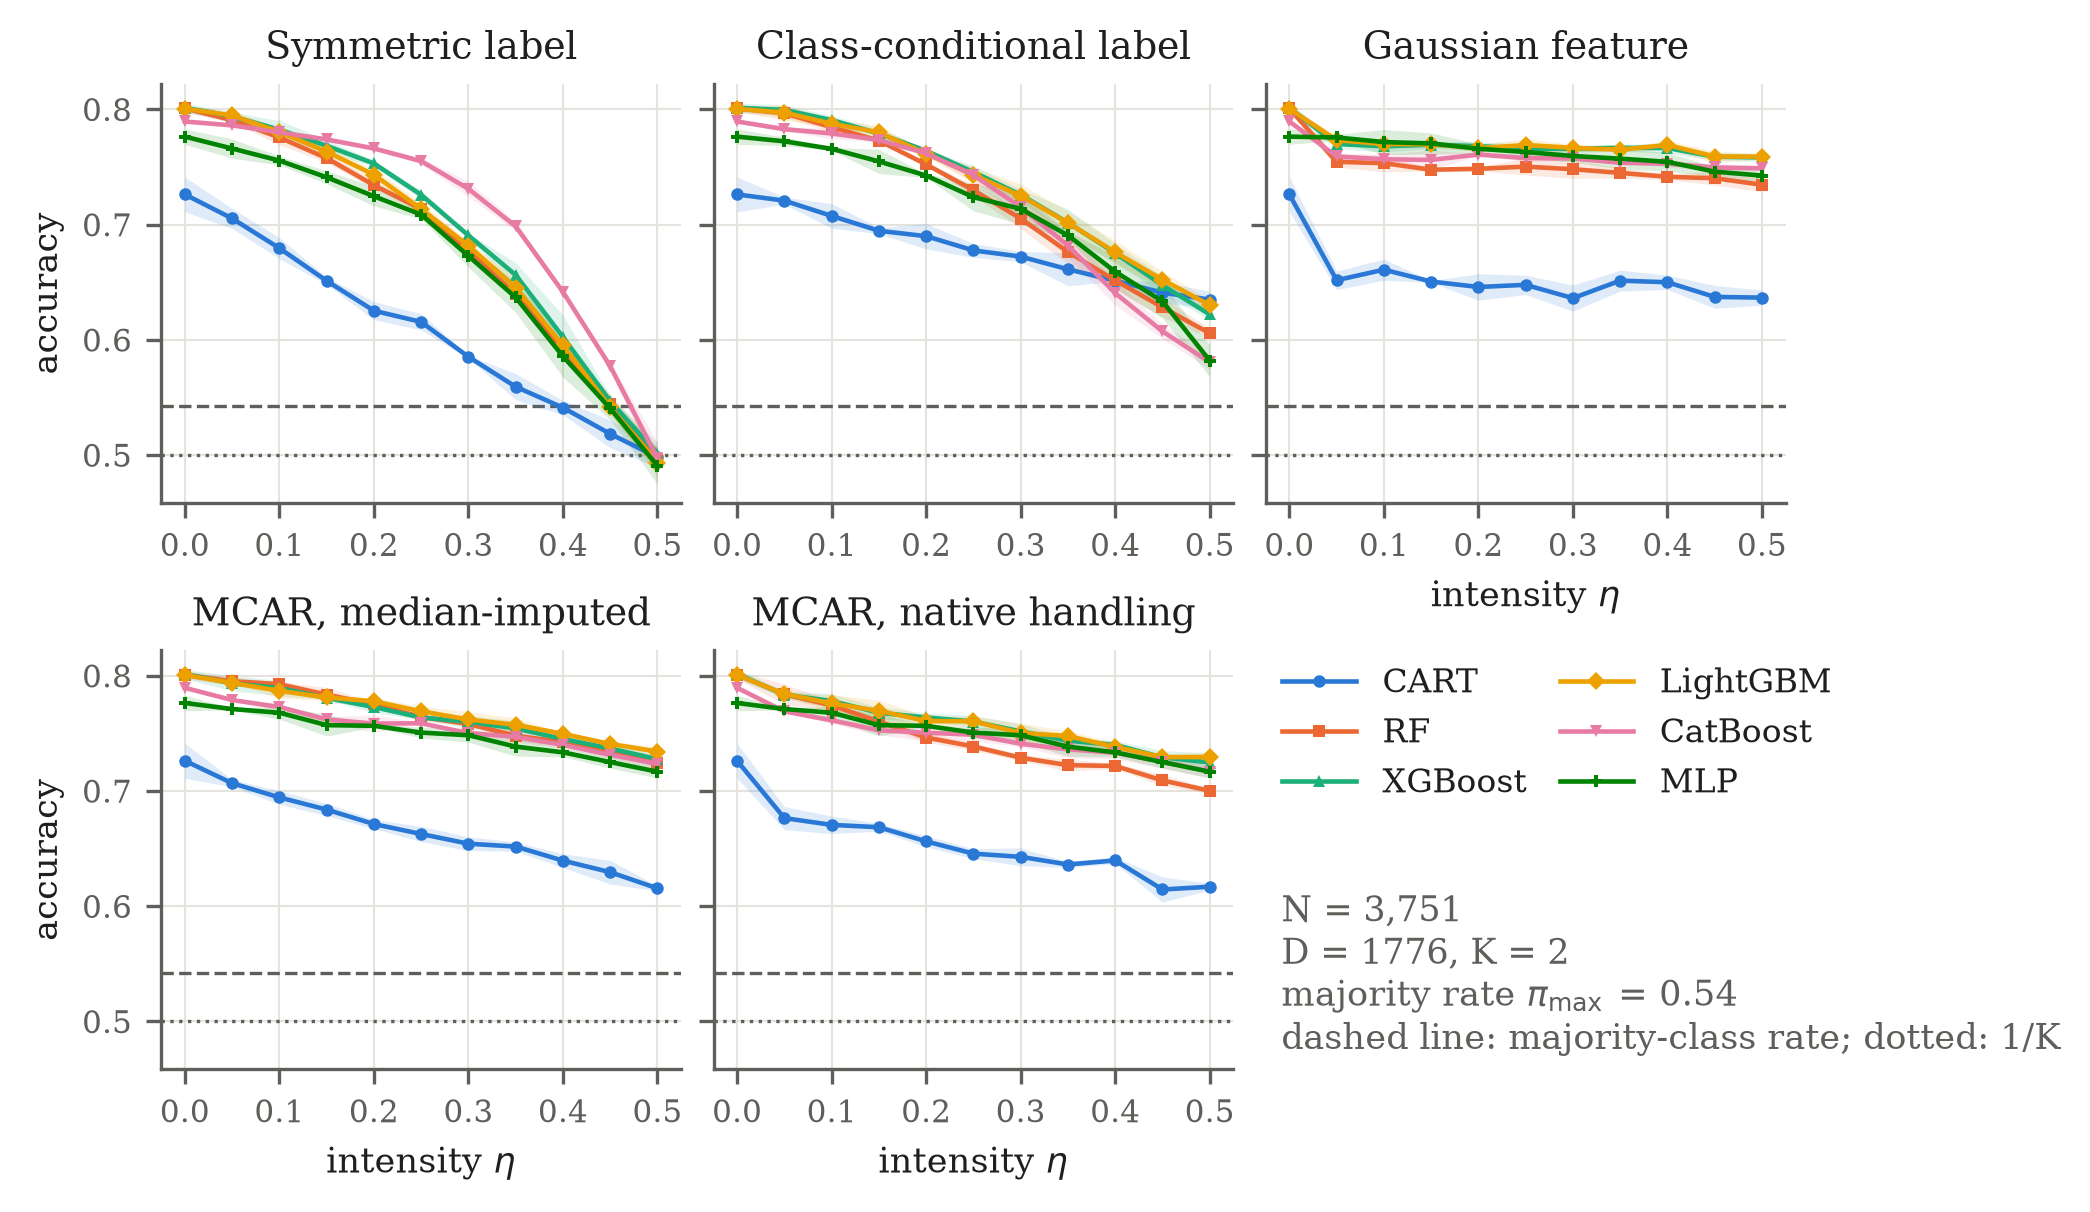
\includegraphics[width=\linewidth]{curves_Bioresponse.png}
  \caption{Bioresponse}\label{fig:atlas_Bioresponse}
\end{subfigure}\\[4pt]
\begin{subfigure}{\linewidth}
  \centering
  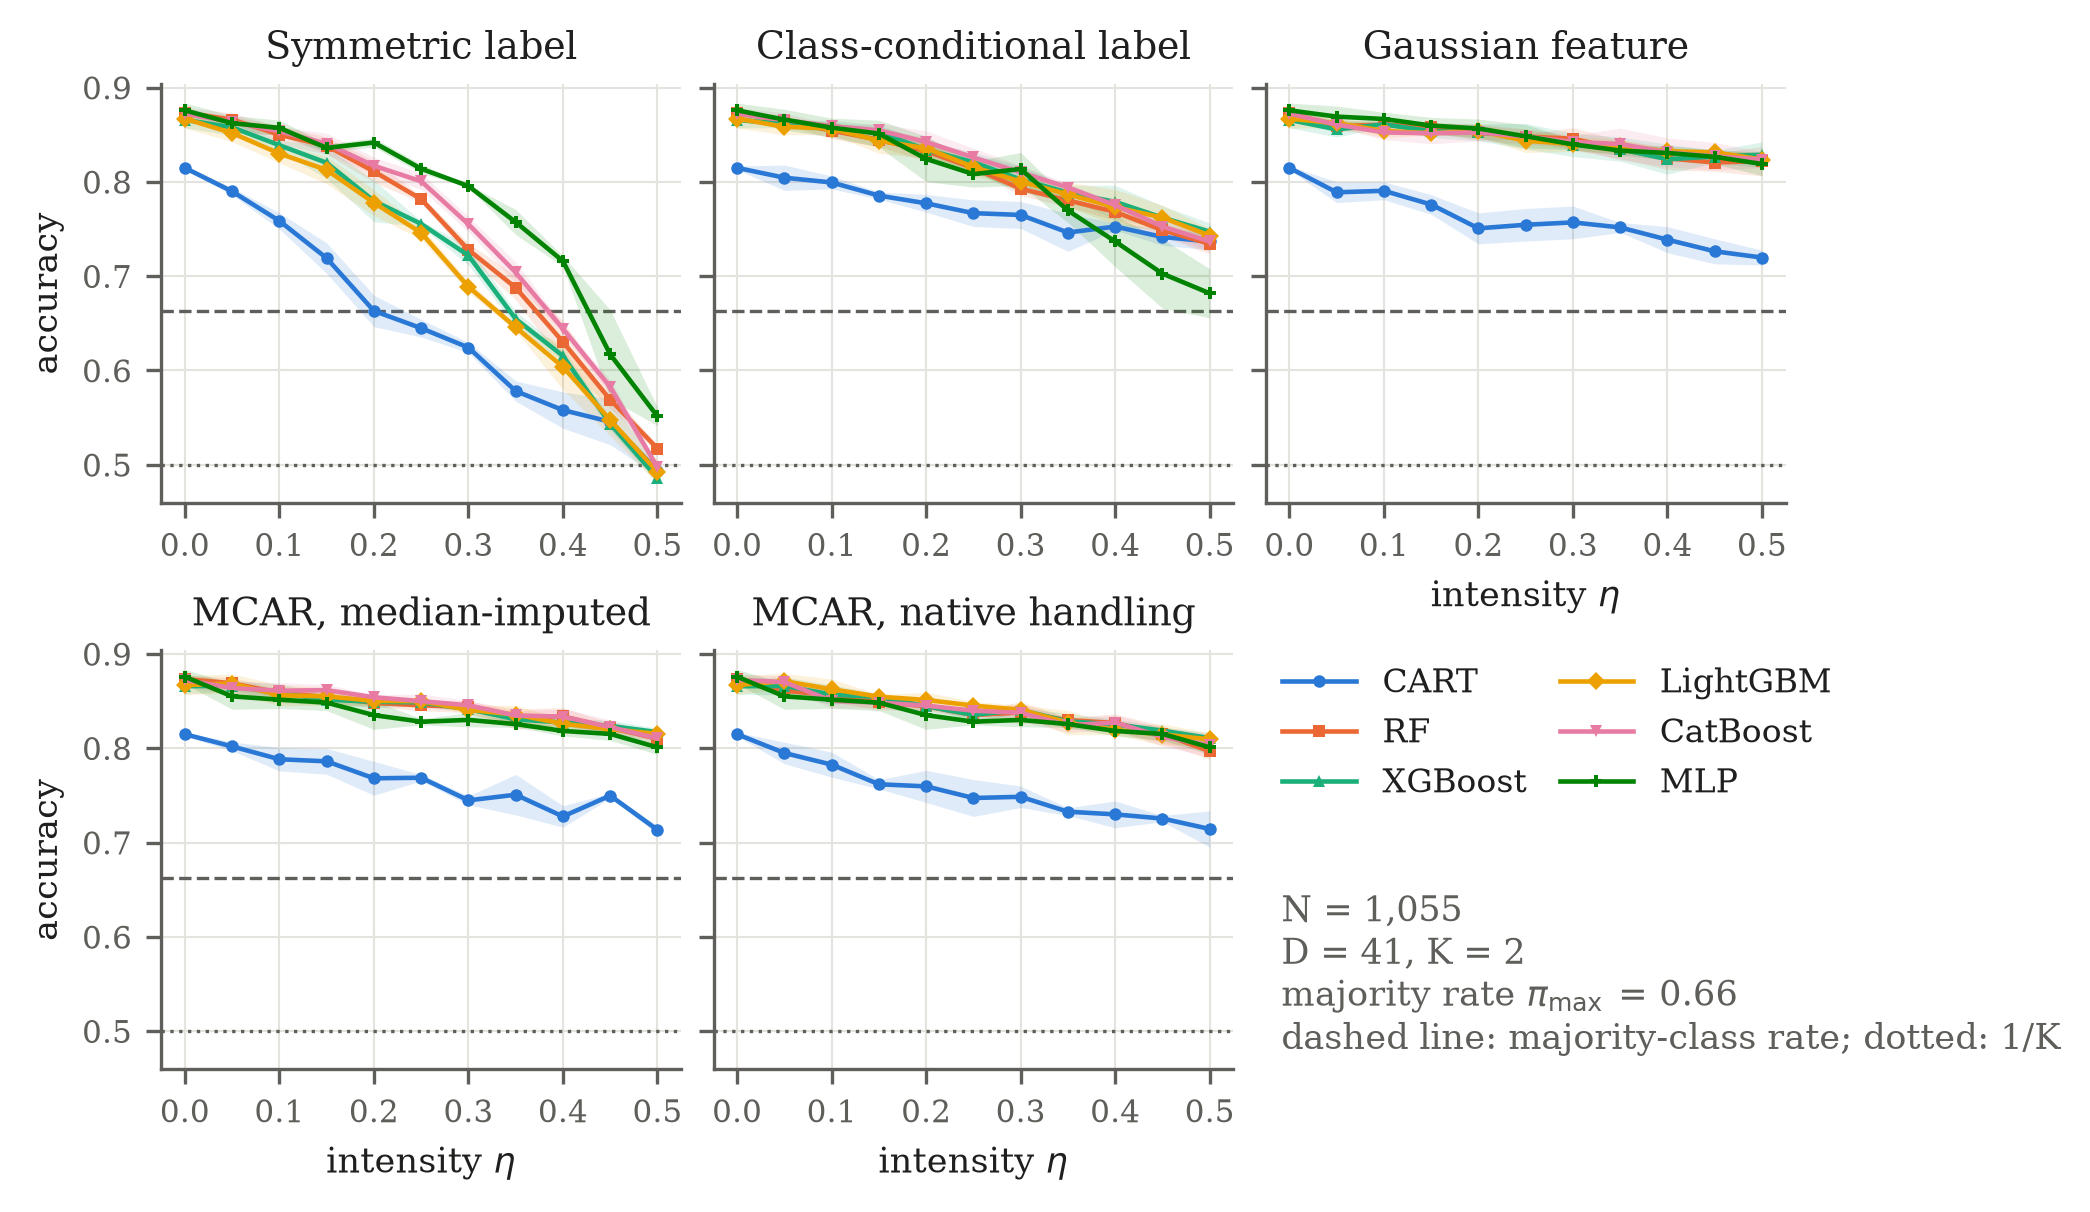
\includegraphics[width=\linewidth]{curves_qsar-biodeg.png}
  \caption{qsar-biodeg}\label{fig:atlas_qsar-biodeg}
\end{subfigure}
\caption{Degradation atlas for chemistry, biology, atmospheric and human-motion sensing. Median MRR of the group: $0.874$ (symmetric label noise), $0.916$ (class-conditional label noise), $0.949$ (Gaussian feature noise), $0.954$ (imputed masking) and $0.937$ (native masking); mean AUDC over its datasets and all five conditions from $0.628$ (CART) to $0.728$ (LightGBM). Band: $\pm1$ sample SD across three seeds; dashed line: $\pi_{\max}$.}
\label{fig:atlas_g1}
\end{figure}

\begin{figure}[tbp]
\ContinuedFloat
\centering
\begin{subfigure}{\linewidth}
  \centering
  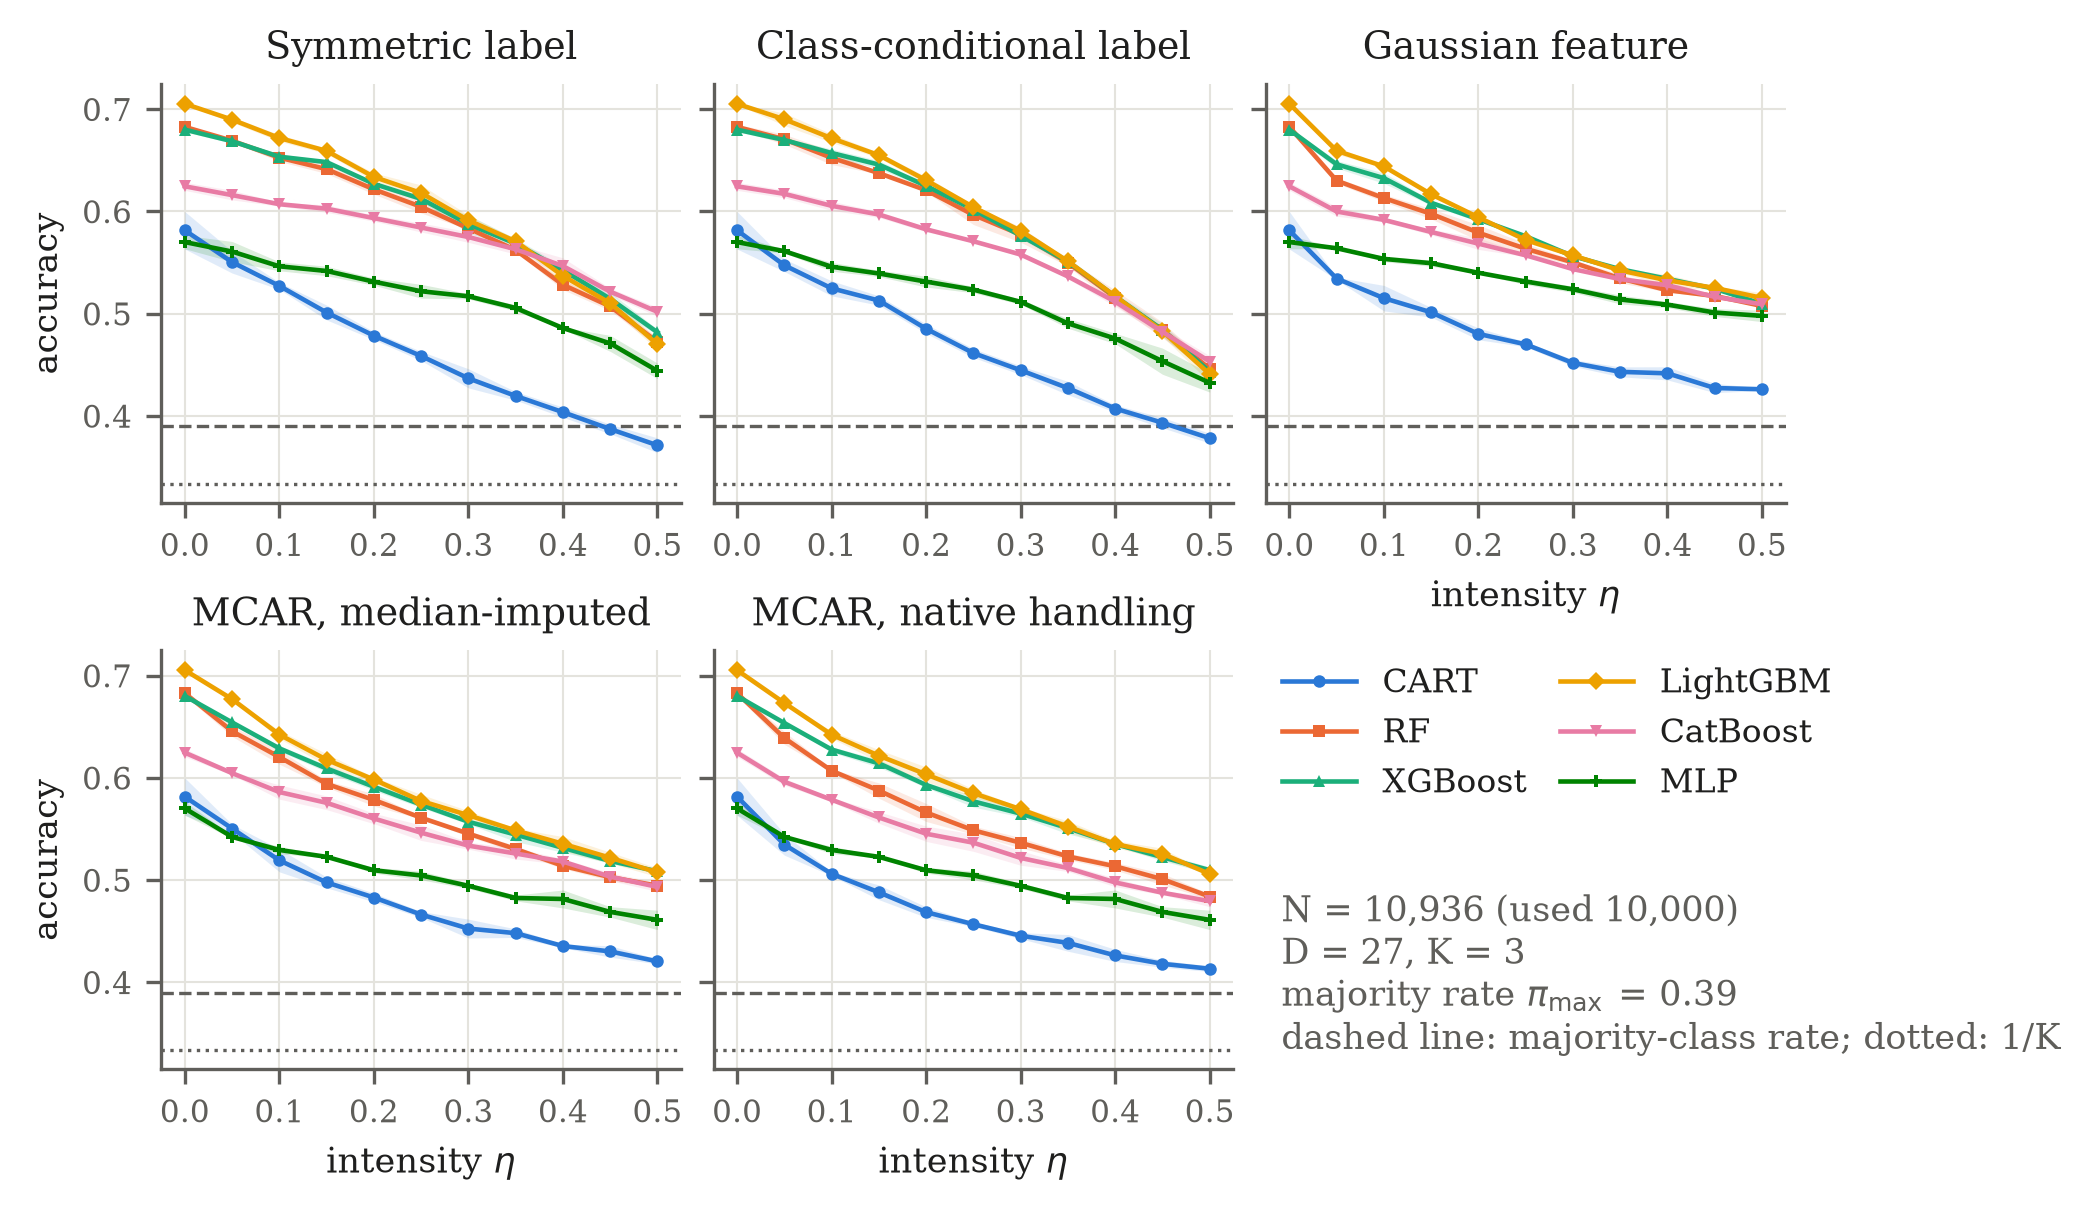
\includegraphics[width=\linewidth]{curves_eye_movements.png}
  \caption{eye\_movements}\label{fig:atlas_eye_movements}
\end{subfigure}\\[4pt]
\begin{subfigure}{\linewidth}
  \centering
  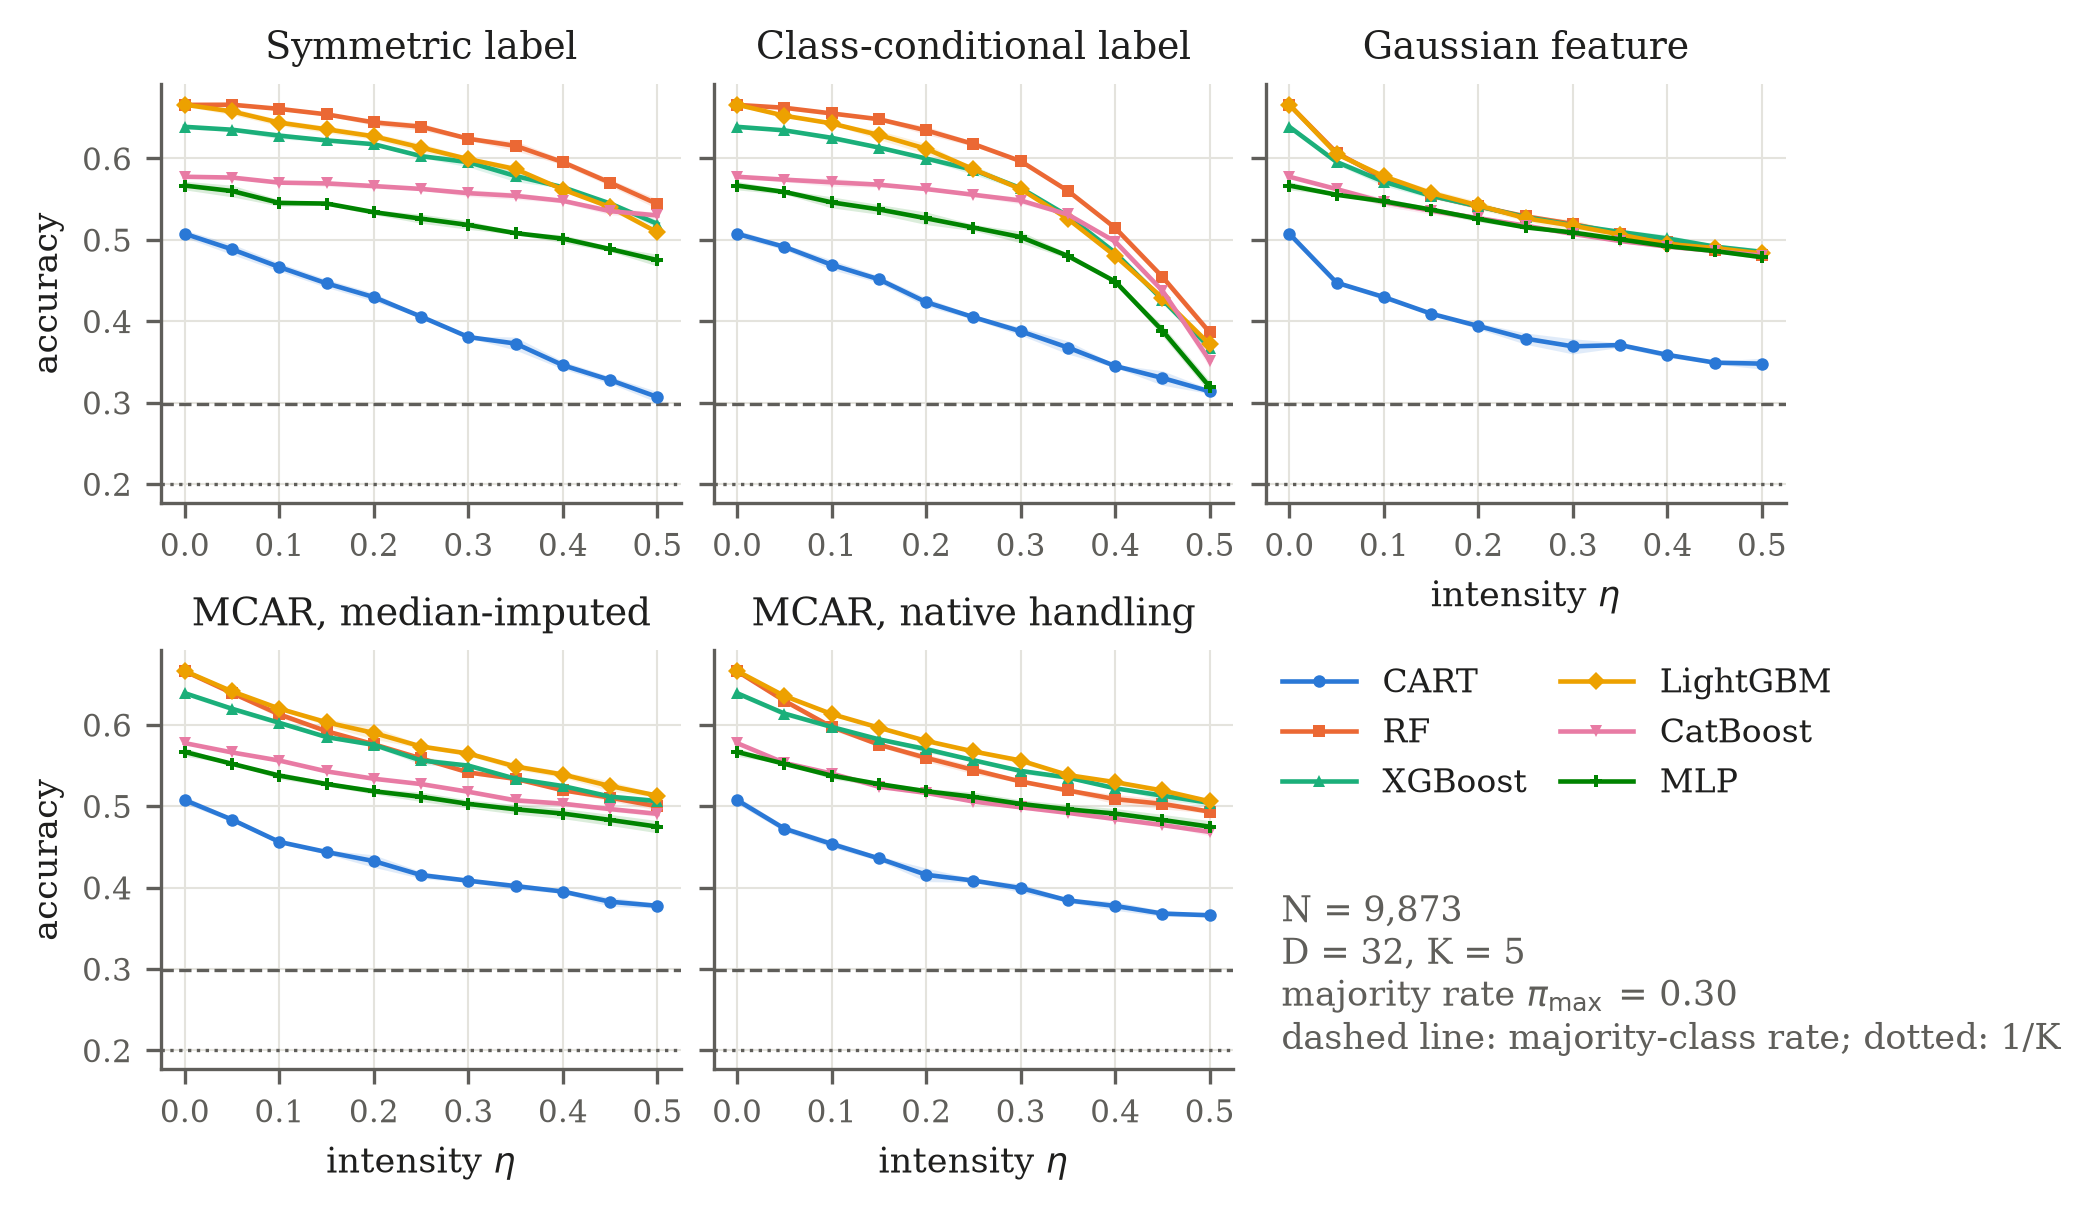
\includegraphics[width=\linewidth]{curves_gesture_phase.png}
  \caption{gesture\_phase}\label{fig:atlas_gesture_phase}
\end{subfigure}
\caption{Degradation atlas for chemistry, biology, atmospheric and human-motion sensing (continued). Band: $\pm1$ sample SD across three seeds; dashed line: $\pi_{\max}$.}
\end{figure}

\begin{figure}[tbp]
\ContinuedFloat
\centering
\begin{subfigure}{\linewidth}
  \centering
  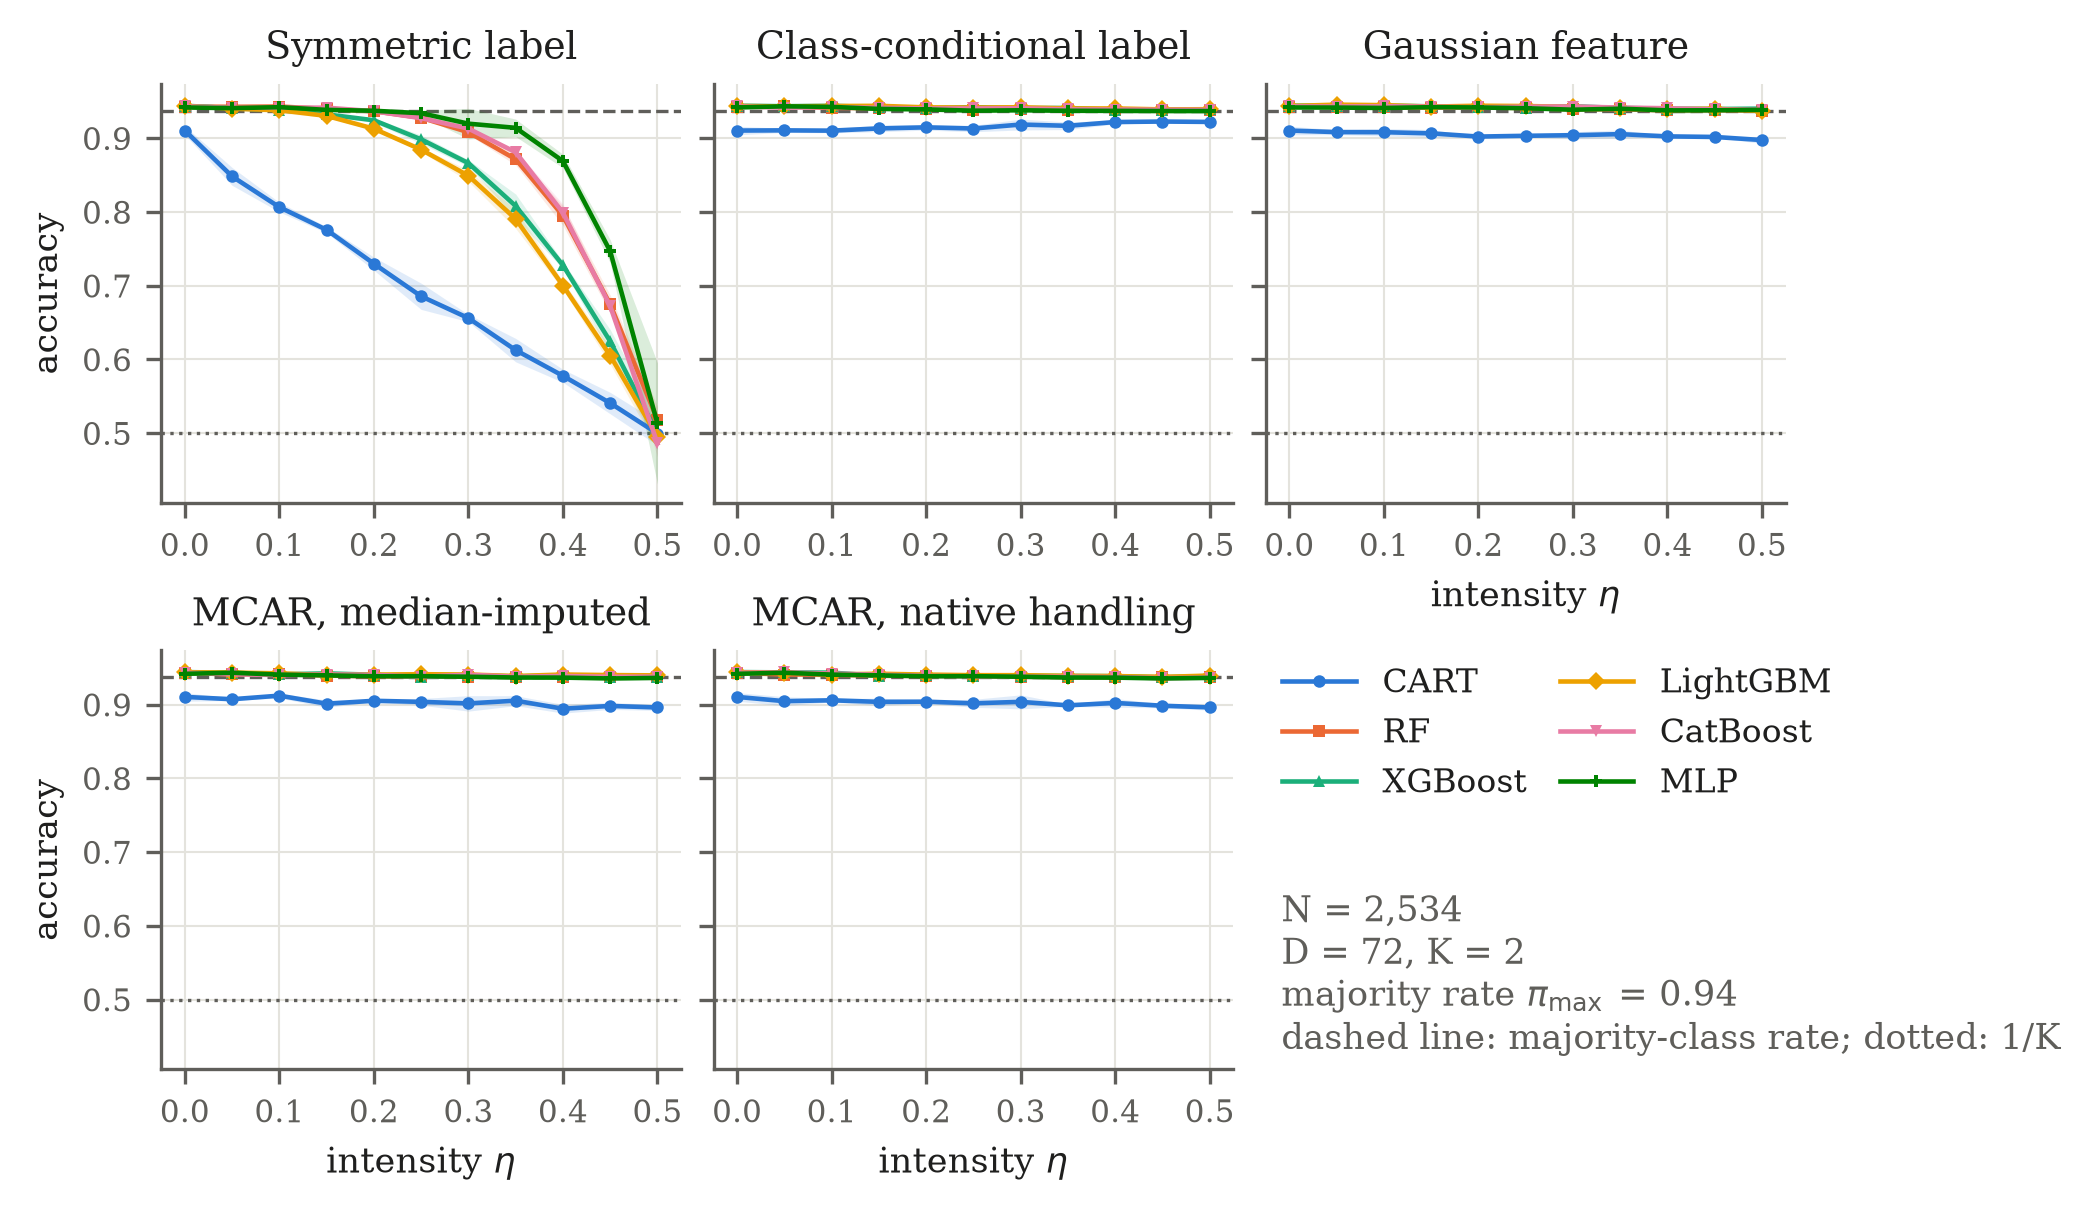
\includegraphics[width=\linewidth]{curves_ozone_level.png}
  \caption{ozone\_level}\label{fig:atlas_ozone_level}
\end{subfigure}
\caption{Degradation atlas for chemistry, biology, atmospheric and human-motion sensing (continued). Band: $\pm1$ sample SD across three seeds; dashed line: $\pi_{\max}$.}
\end{figure}

\begin{figure}[tbp]

\centering
\begin{subfigure}{\linewidth}
  \centering
  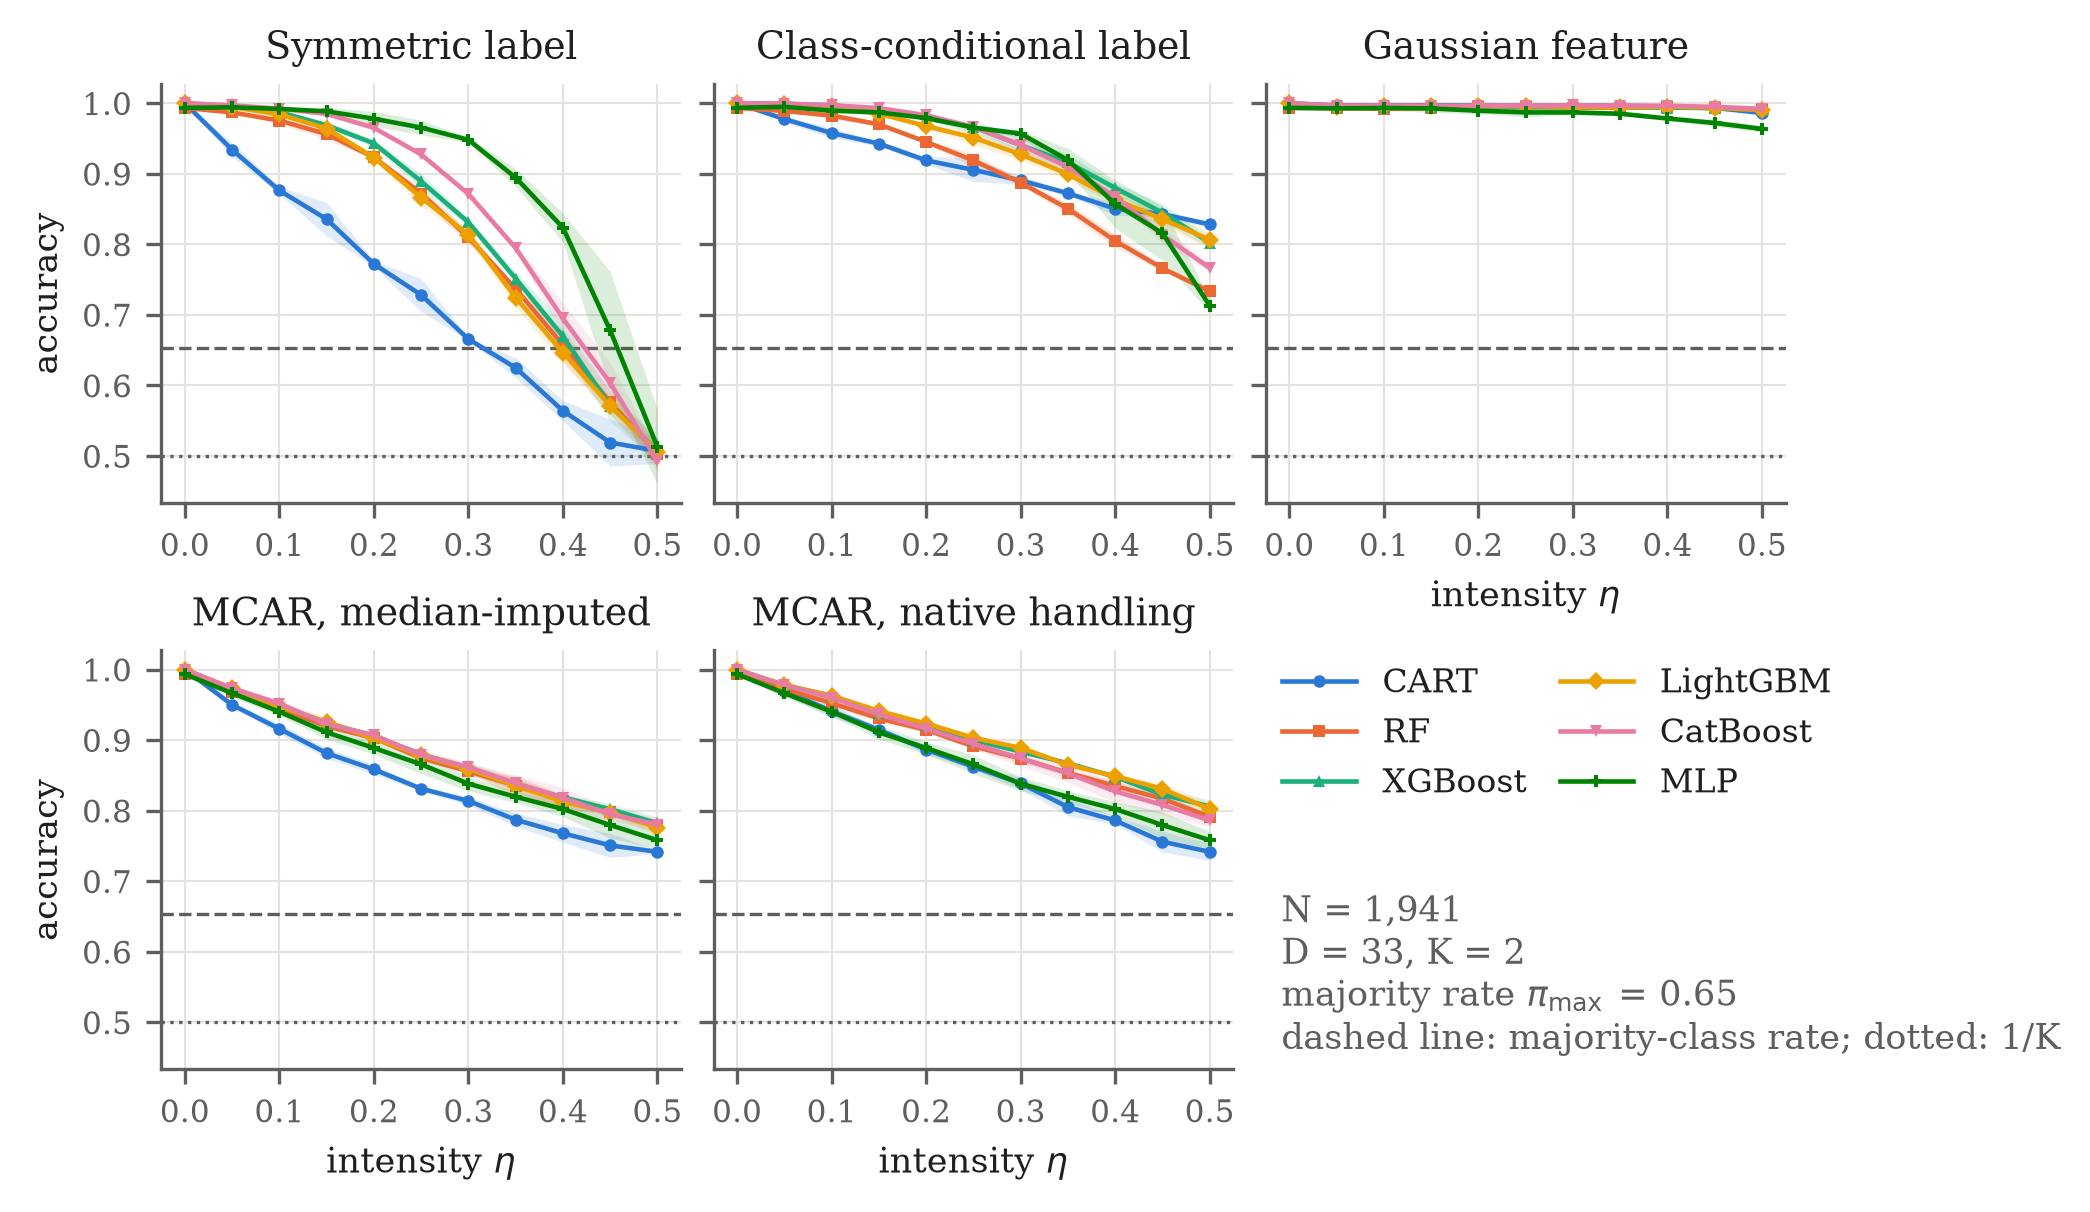
\includegraphics[width=\linewidth]{curves_steel-plates-fault.png}
  \caption{steel-plates-fault}\label{fig:atlas_steel-plates-fault}
\end{subfigure}\\[4pt]
\begin{subfigure}{\linewidth}
  \centering
  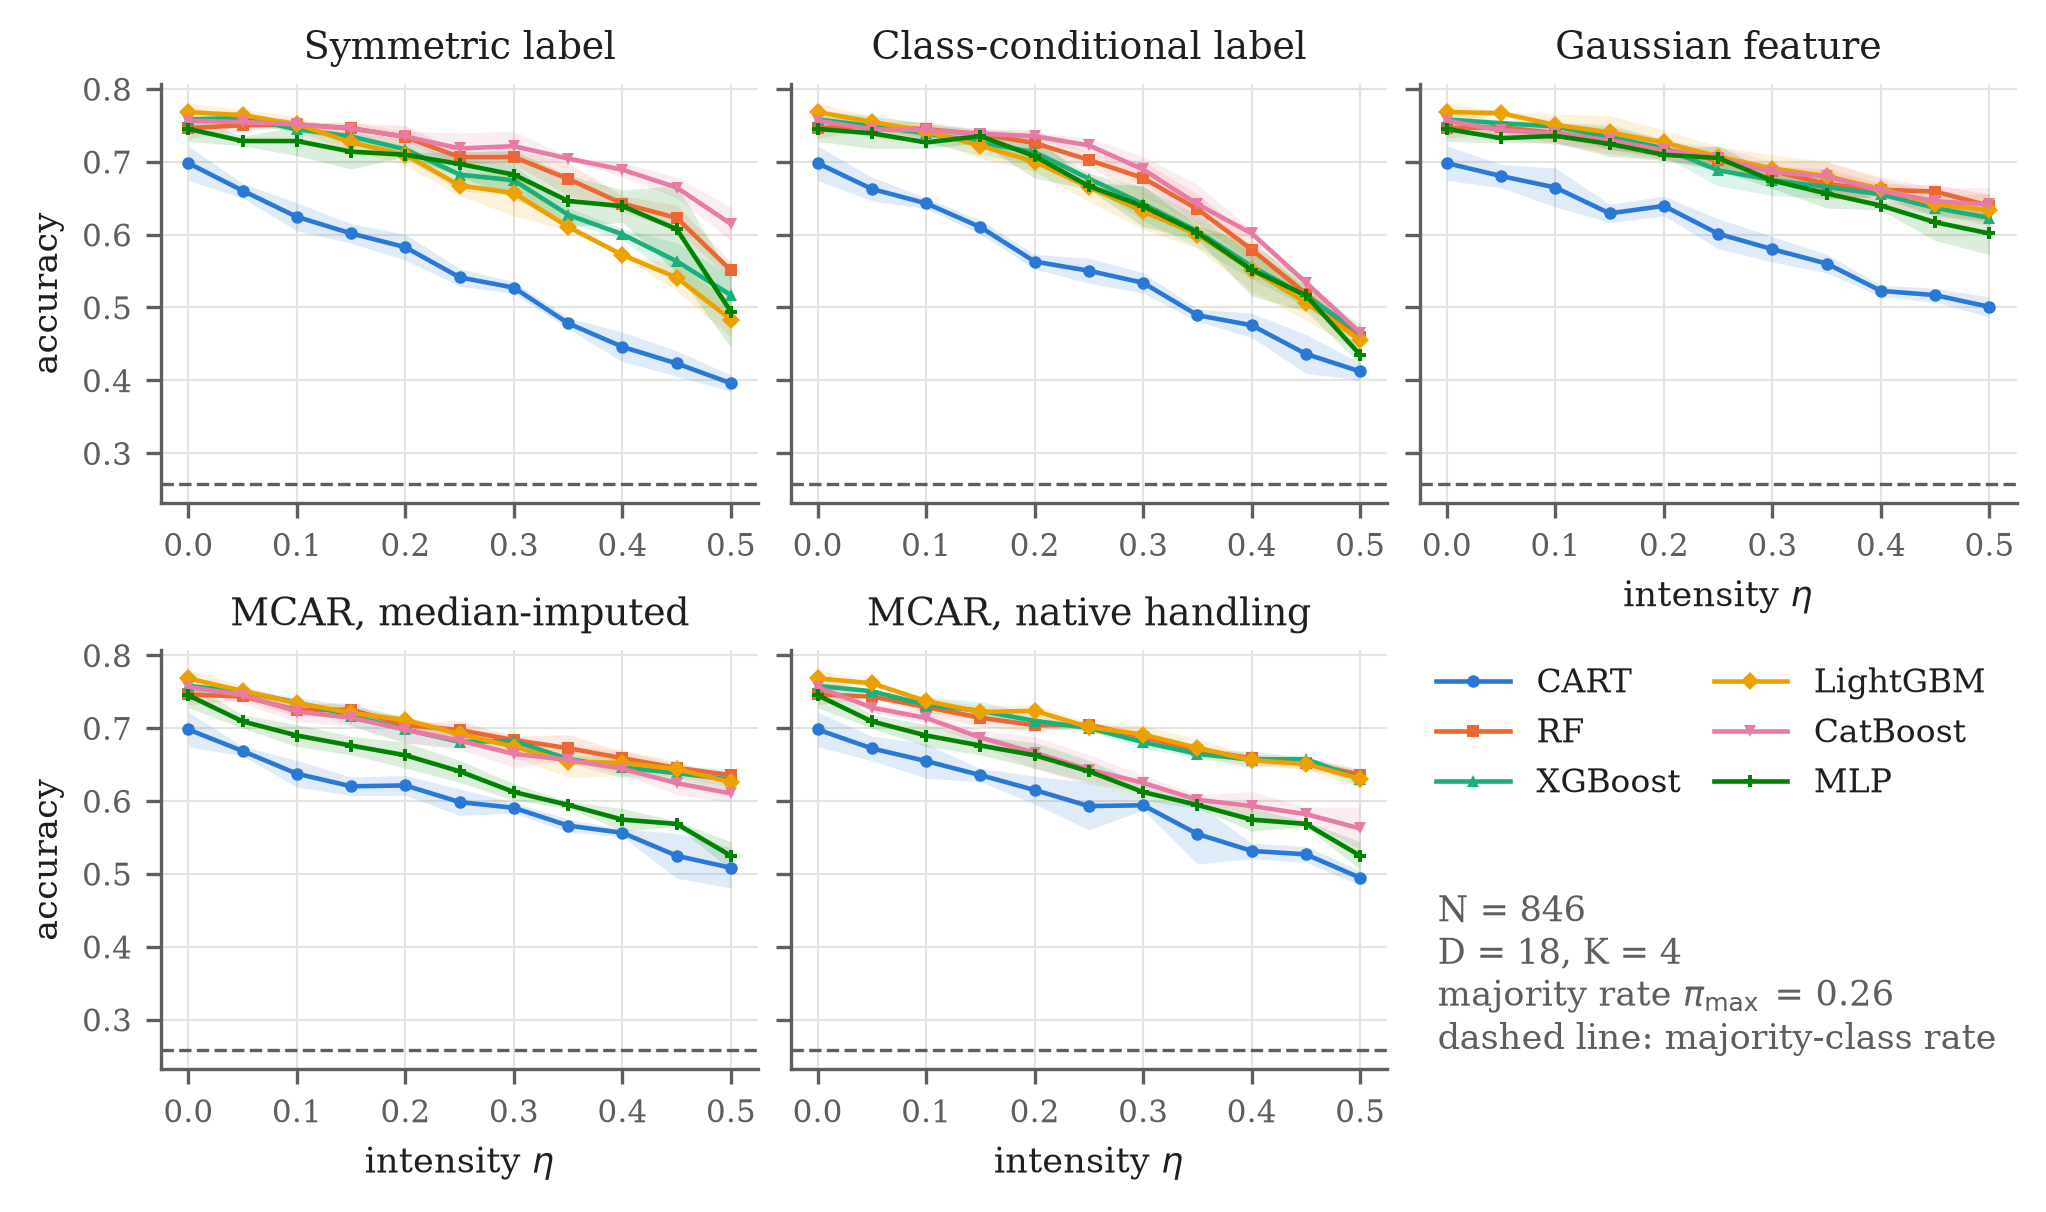
\includegraphics[width=\linewidth]{curves_vehicle.png}
  \caption{vehicle}\label{fig:atlas_vehicle}
\end{subfigure}
\caption{Degradation atlas for industrial, physical and network measurements. Median MRR of the group: $0.904$ (symmetric label noise), $0.921$ (class-conditional label noise), $0.926$ (Gaussian feature noise), $0.910$ (imputed masking) and $0.914$ (native masking); mean AUDC over its datasets and all five conditions from $0.729$ (CART) to $0.813$ (XGBoost). Band: $\pm1$ sample SD across three seeds; dashed line: $\pi_{\max}$.}
\label{fig:atlas_g2}
\end{figure}

\begin{figure}[tbp]
\ContinuedFloat
\centering
\begin{subfigure}{\linewidth}
  \centering
  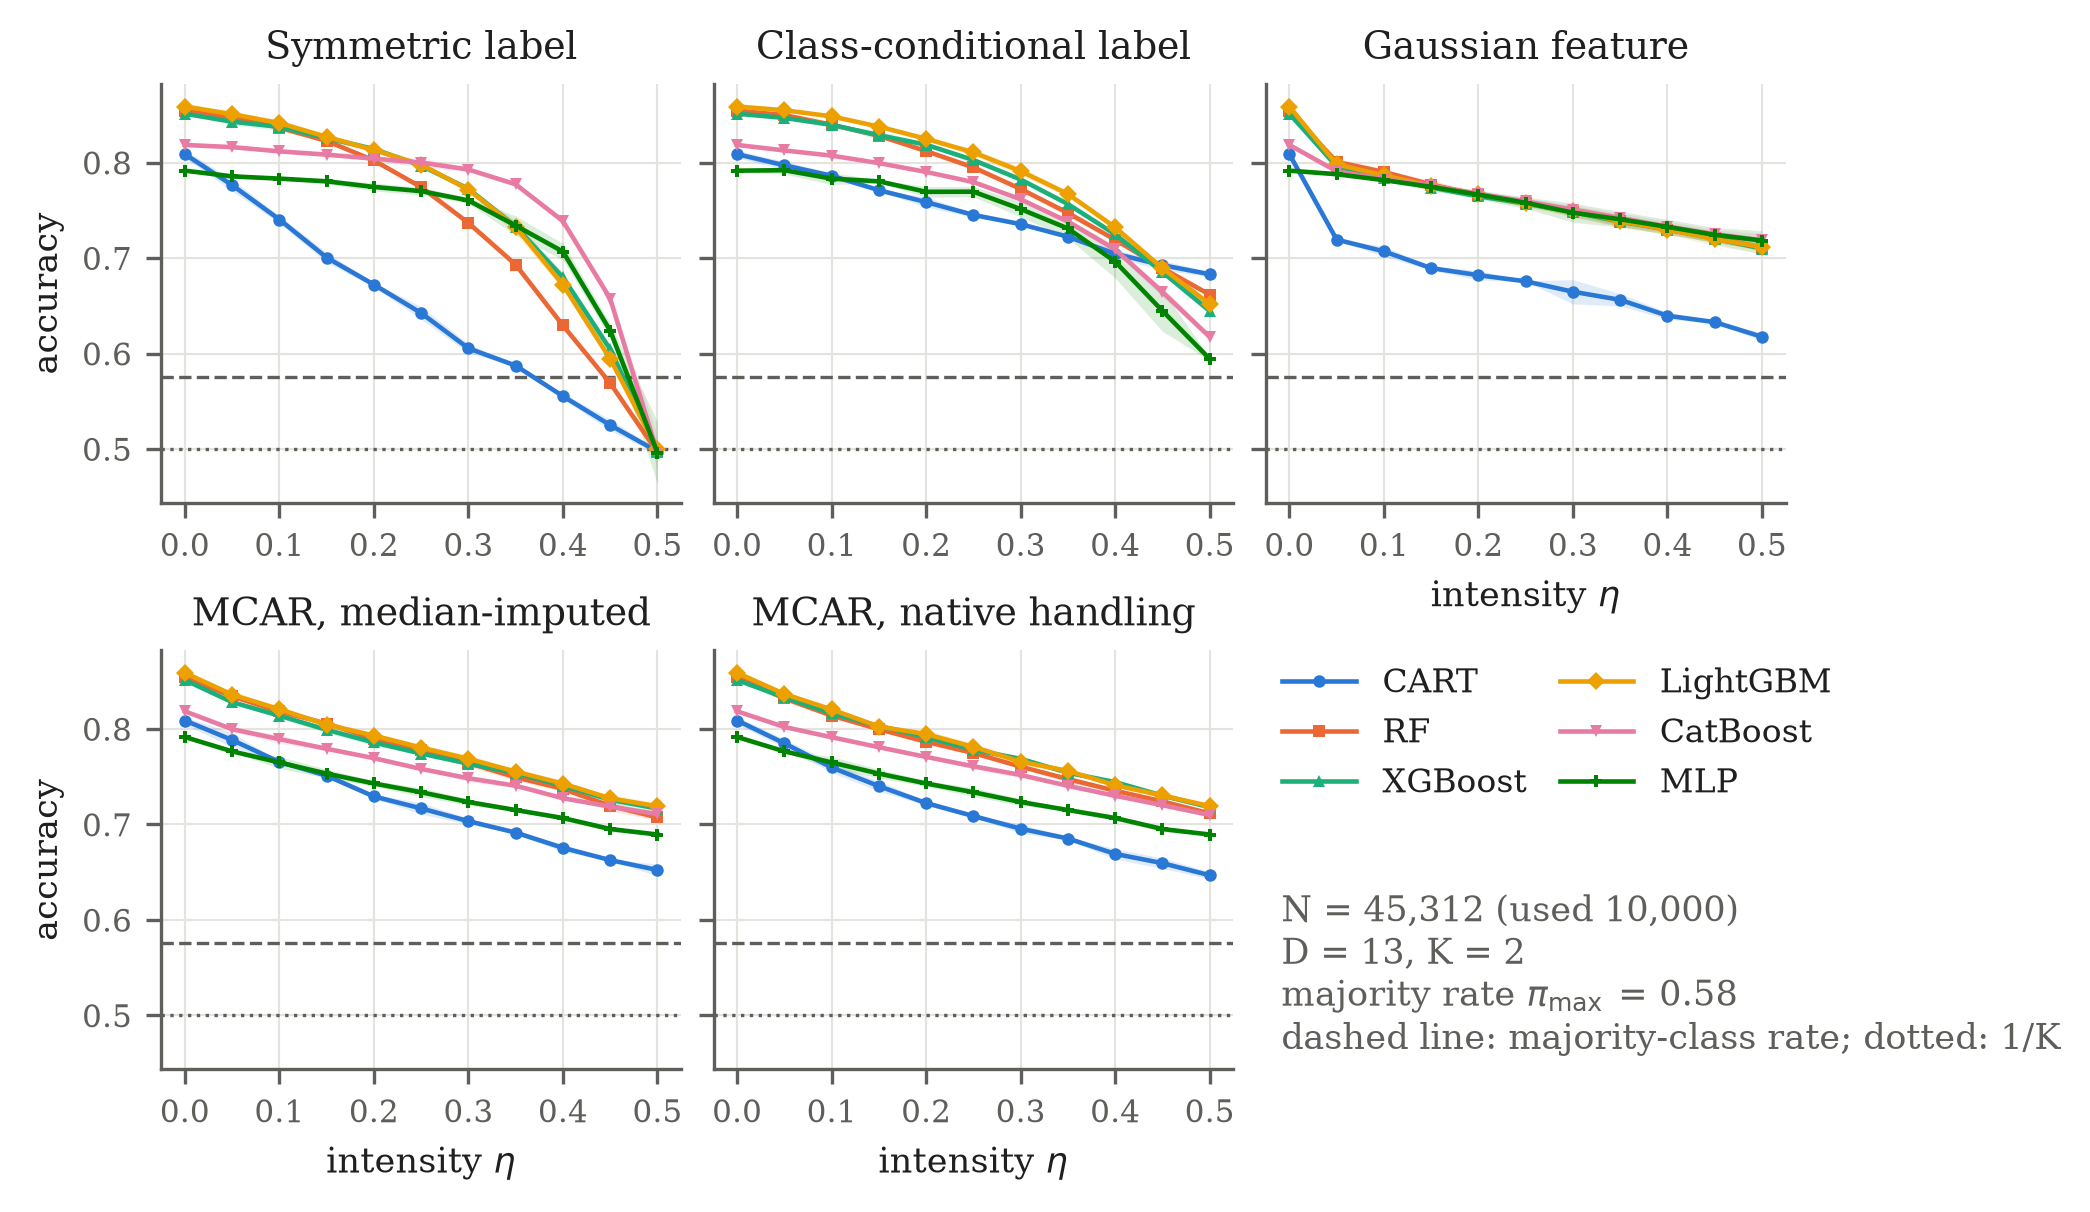
\includegraphics[width=\linewidth]{curves_electricity.png}
  \caption{electricity}\label{fig:atlas_electricity}
\end{subfigure}\\[4pt]
\begin{subfigure}{\linewidth}
  \centering
  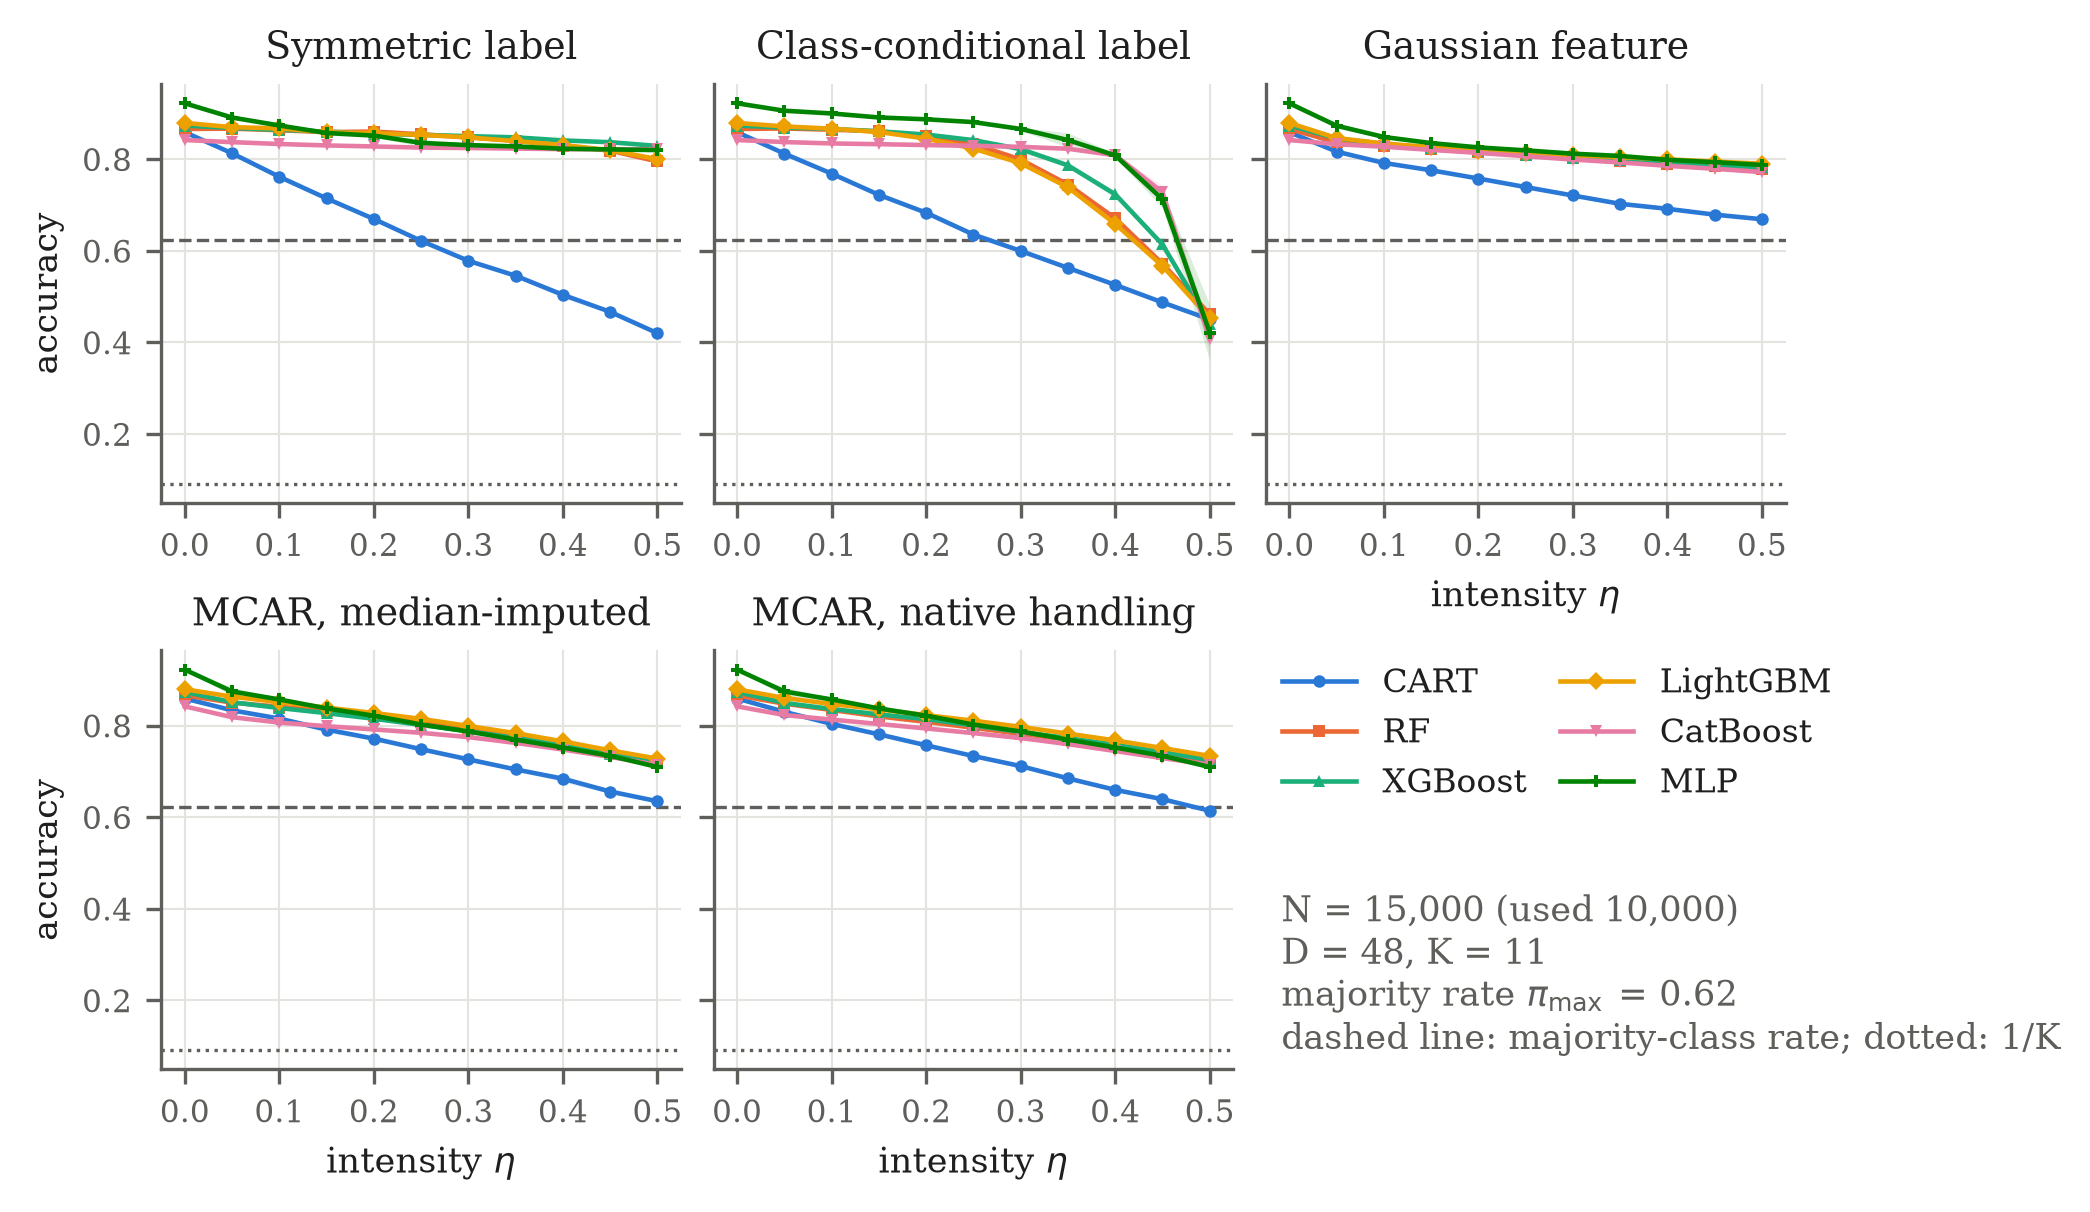
\includegraphics[width=\linewidth]{curves_pol.png}
  \caption{pol}\label{fig:atlas_pol}
\end{subfigure}
\caption{Degradation atlas for industrial, physical and network measurements (continued). Band: $\pm1$ sample SD across three seeds; dashed line: $\pi_{\max}$.}
\end{figure}

\begin{figure}[tbp]
\ContinuedFloat
\centering
\begin{subfigure}{\linewidth}
  \centering
  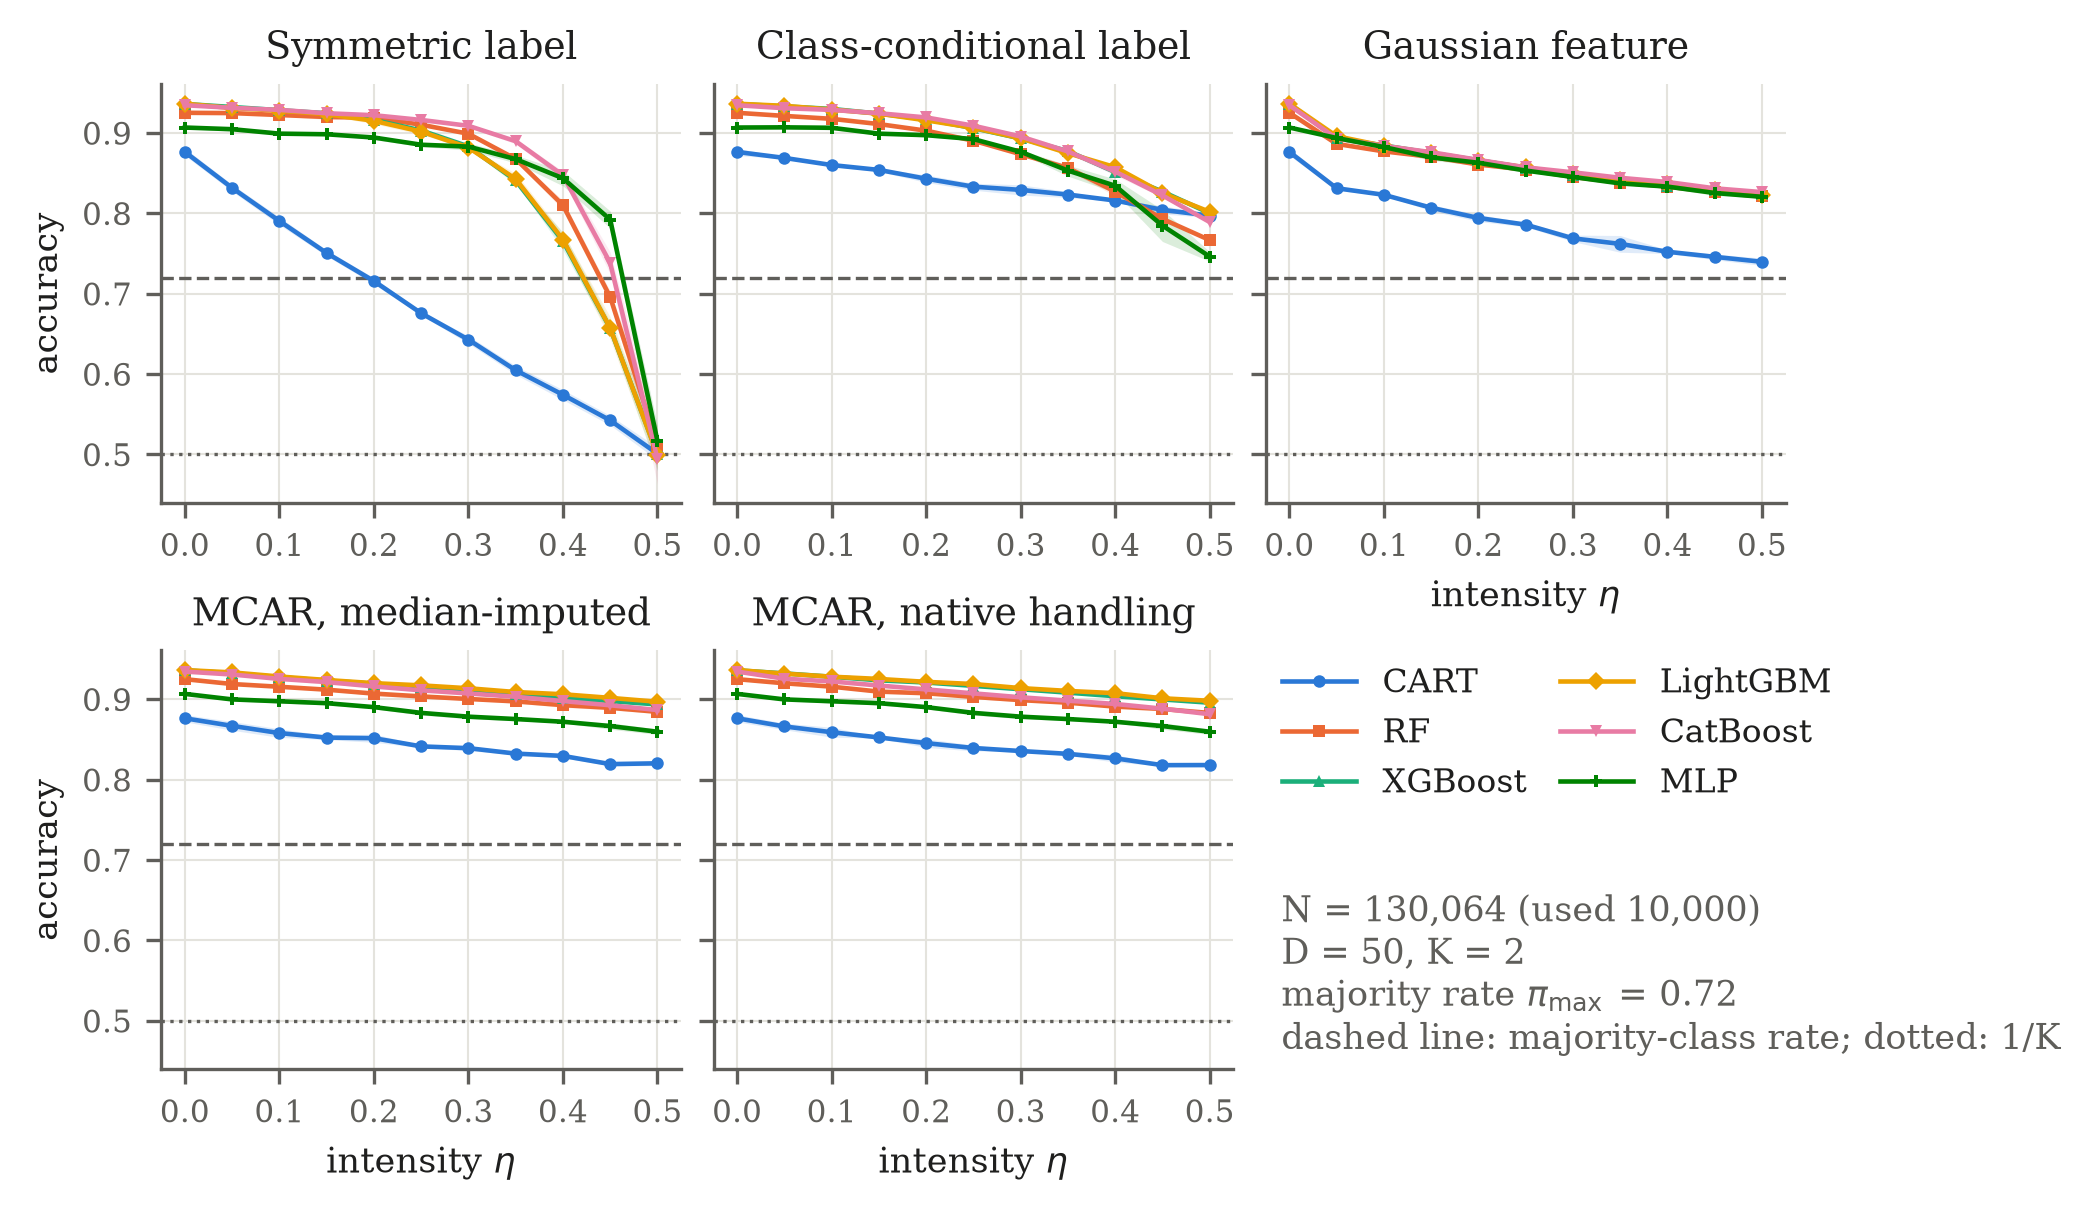
\includegraphics[width=\linewidth]{curves_miniboone.png}
  \caption{miniboone}\label{fig:atlas_miniboone}
\end{subfigure}
\caption{Degradation atlas for industrial, physical and network measurements (continued). Band: $\pm1$ sample SD across three seeds; dashed line: $\pi_{\max}$.}
\end{figure}

\begin{figure}[tbp]

\centering
\begin{subfigure}{\linewidth}
  \centering
  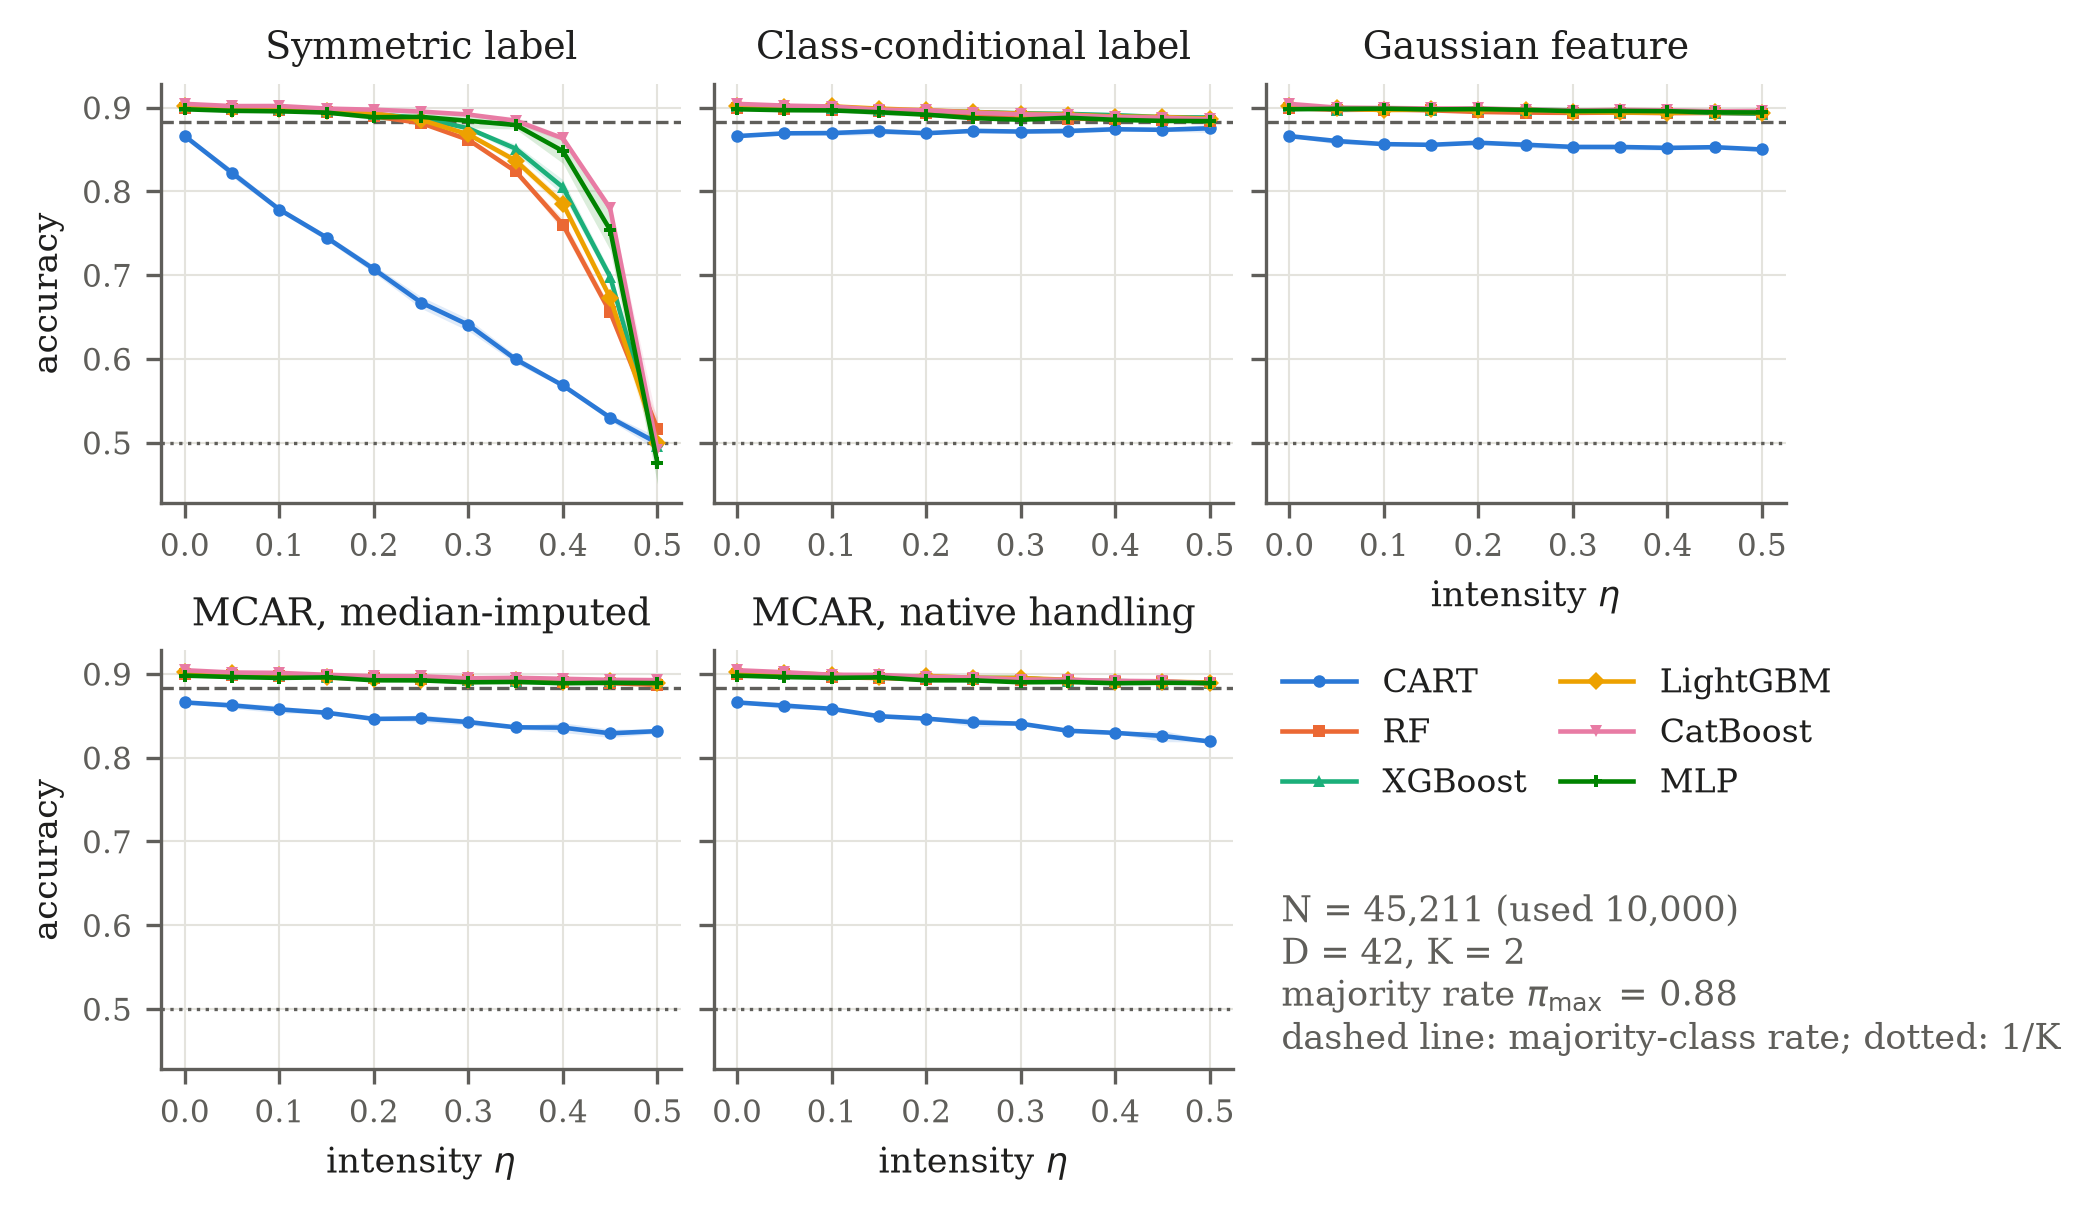
\includegraphics[width=\linewidth]{curves_bank-marketing.png}
  \caption{bank-marketing}\label{fig:atlas_bank-marketing}
\end{subfigure}\\[4pt]
\begin{subfigure}{\linewidth}
  \centering
  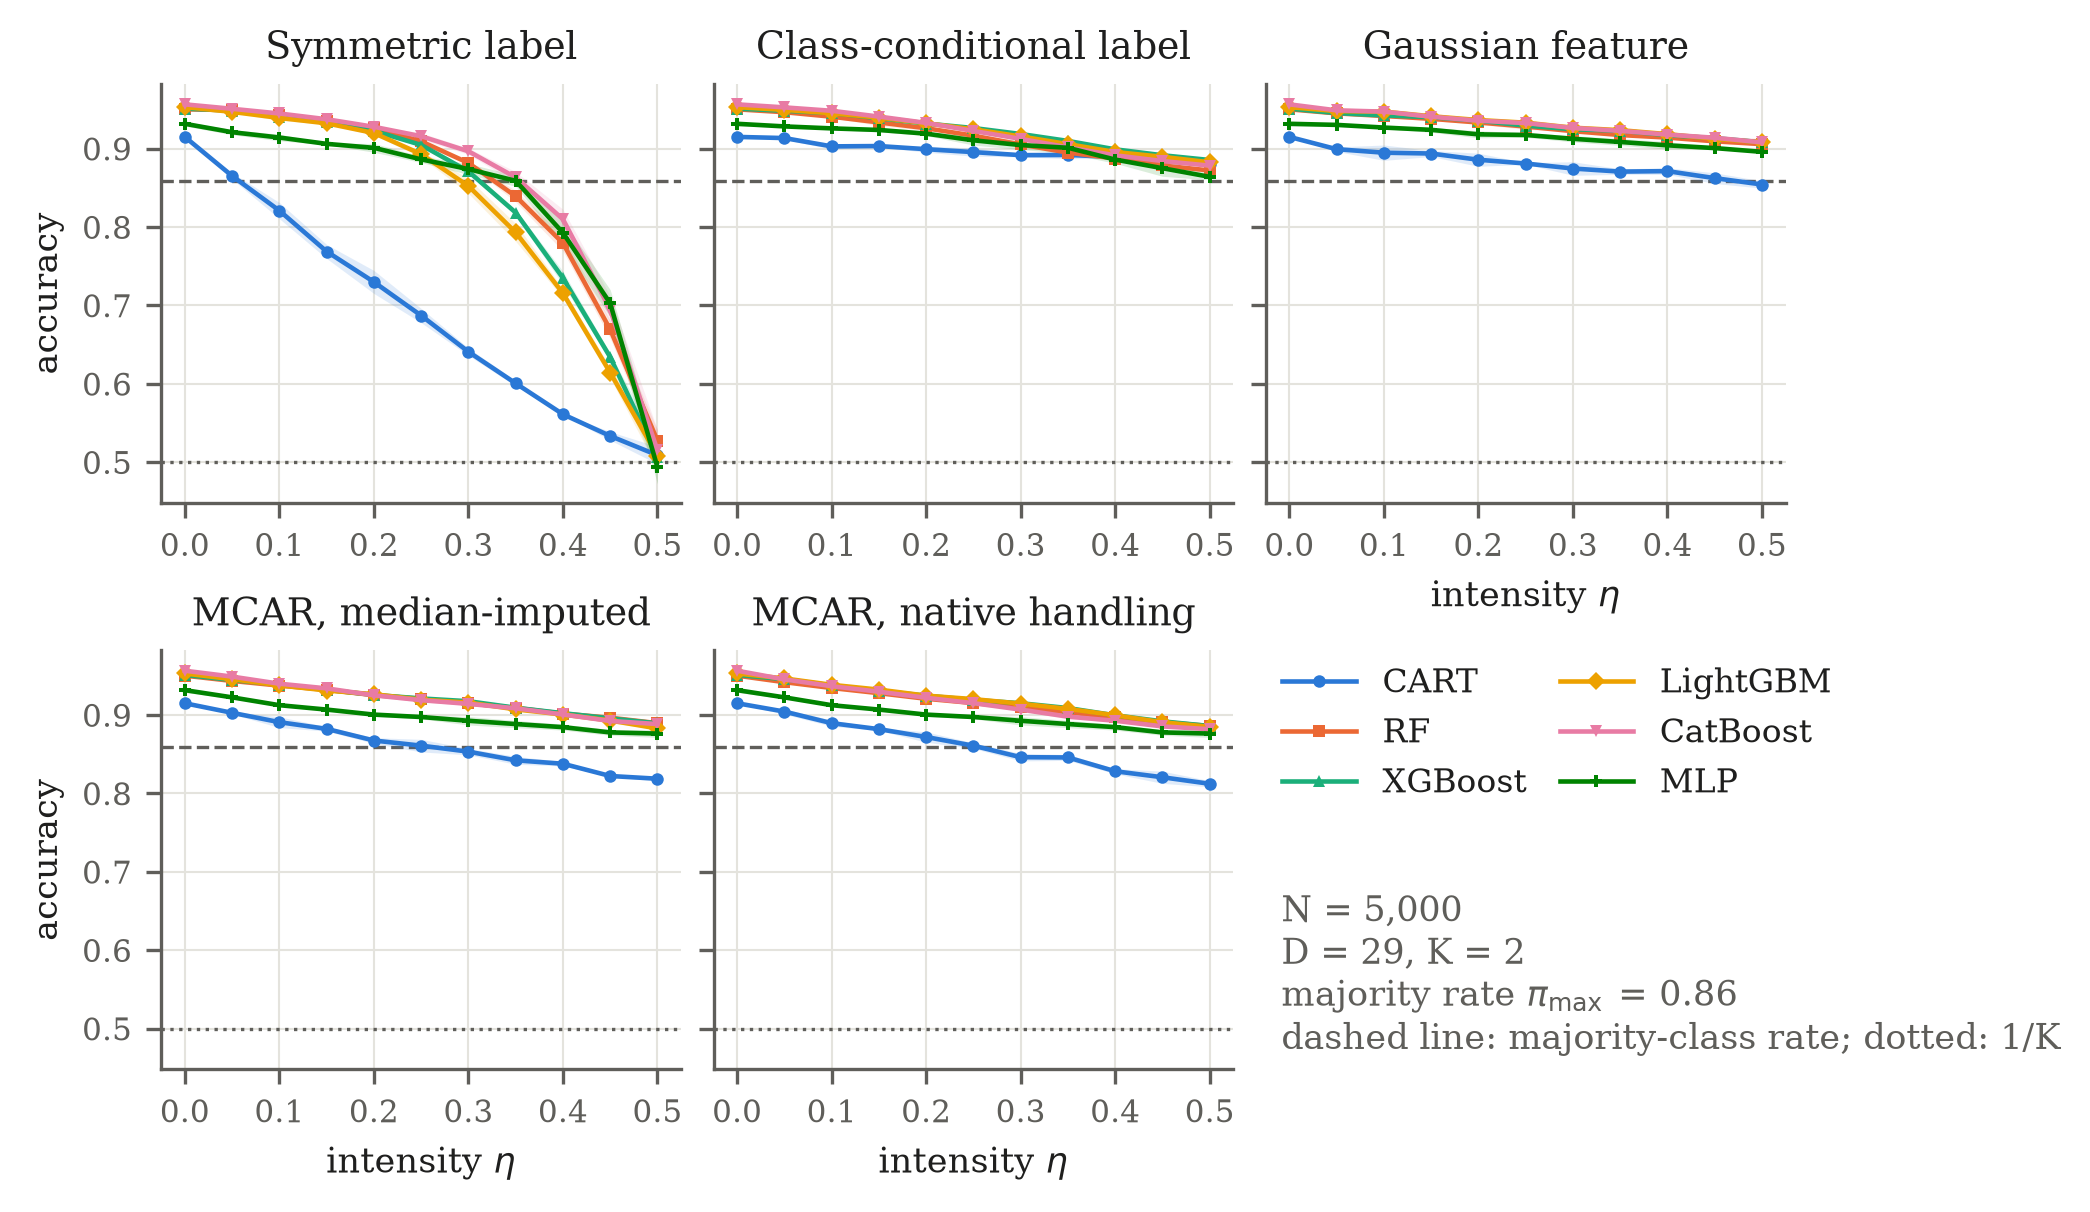
\includegraphics[width=\linewidth]{curves_churn.png}
  \caption{churn}\label{fig:atlas_churn}
\end{subfigure}
\caption{Degradation atlas for business, marketing and web data. Median MRR of the group: $0.908$ (symmetric label noise), $0.970$ (class-conditional label noise), $0.988$ (Gaussian feature noise), $0.981$ (imputed masking) and $0.980$ (native masking); mean AUDC over its datasets and all five conditions from $0.839$ (CART) to $0.915$ (CatBoost). Band: $\pm1$ sample SD across three seeds; dashed line: $\pi_{\max}$.}
\label{fig:atlas_g3}
\end{figure}

\begin{figure}[tbp]
\ContinuedFloat
\centering
\begin{subfigure}{\linewidth}
  \centering
  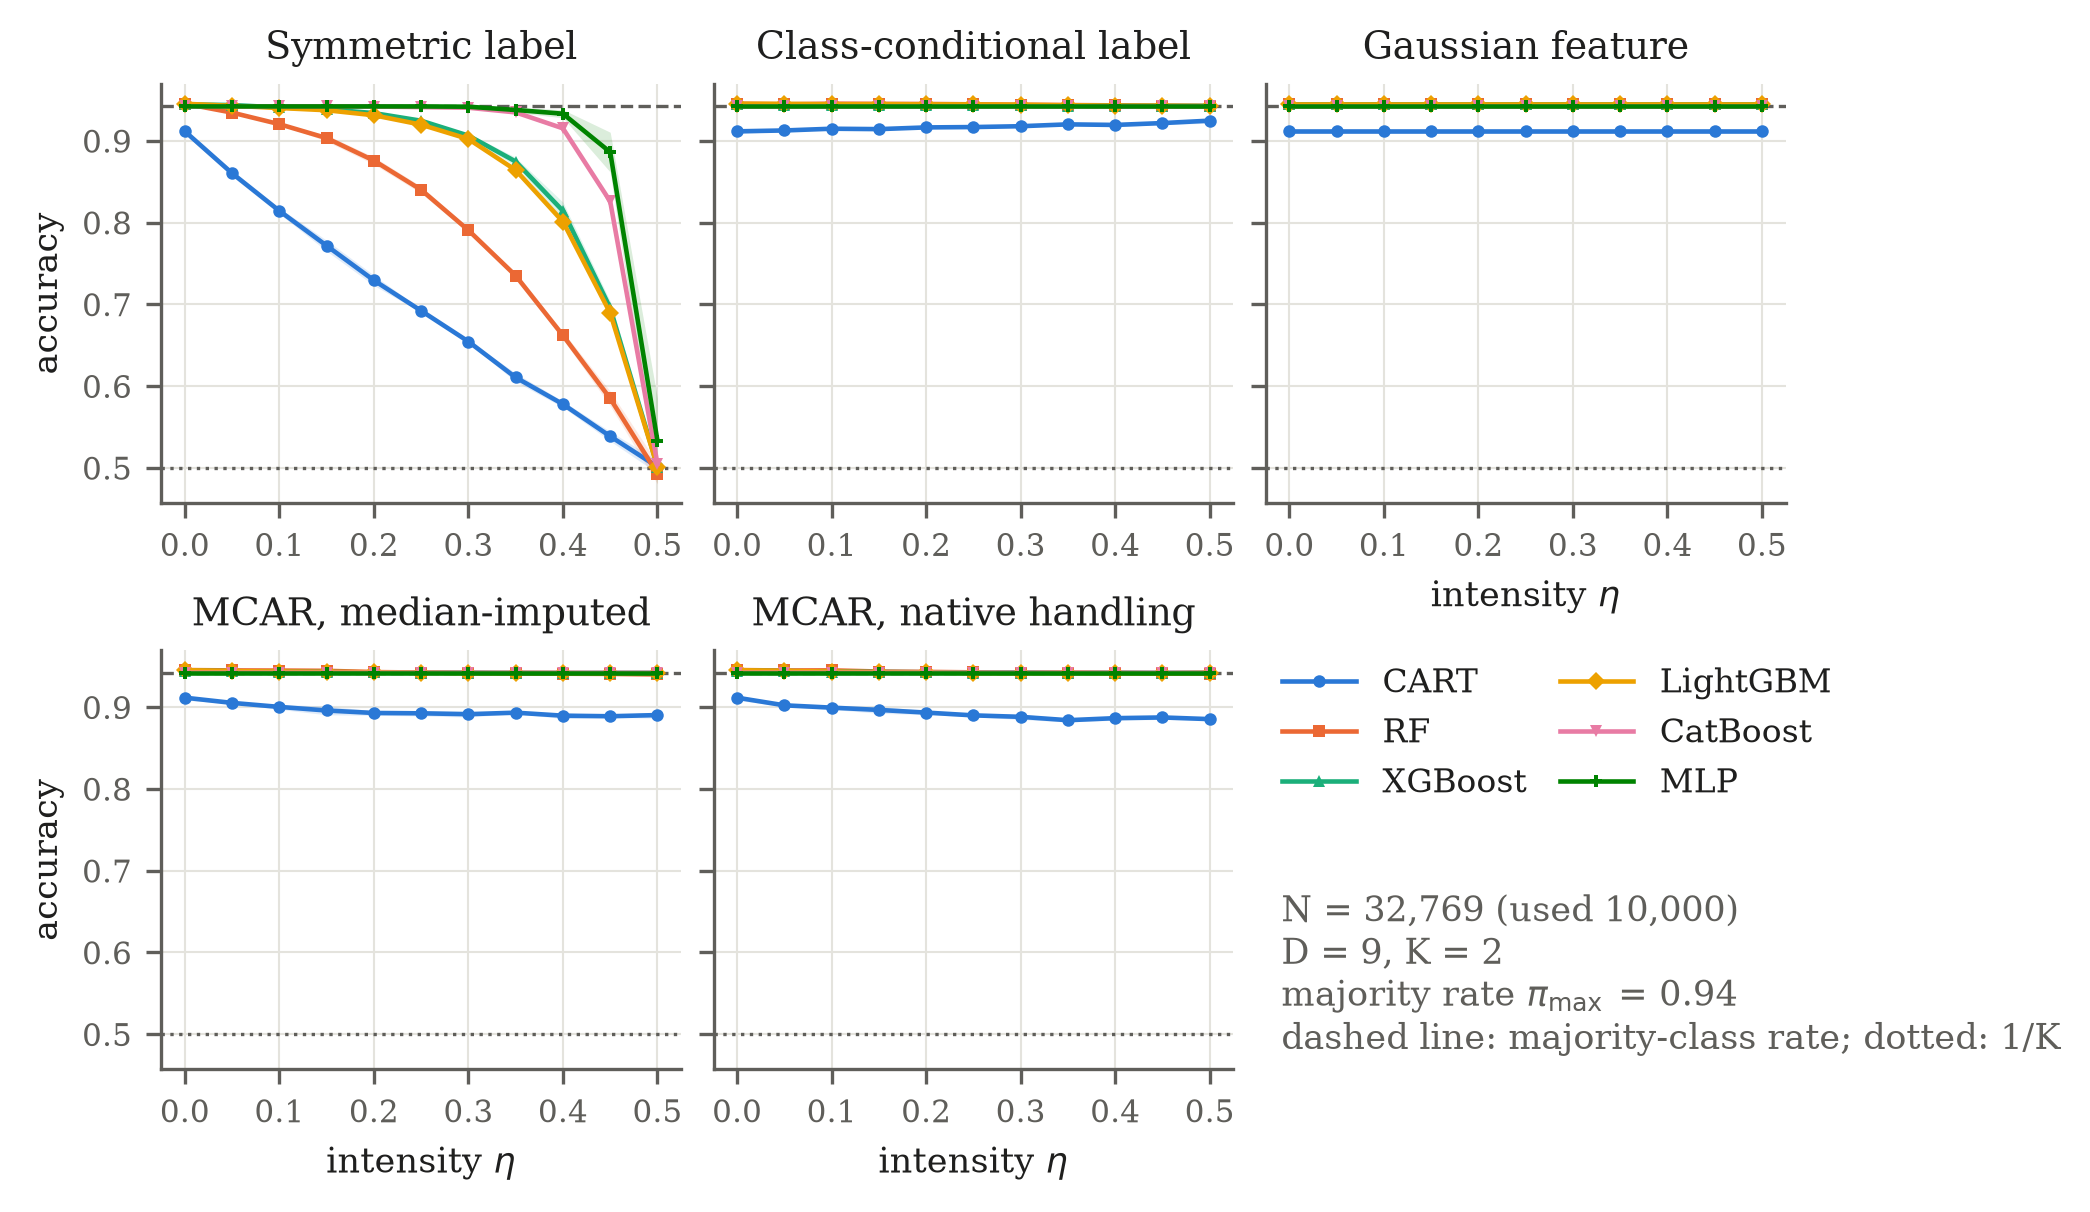
\includegraphics[width=\linewidth]{curves_amazon_access.png}
  \caption{amazon\_access}\label{fig:atlas_amazon_access}
\end{subfigure}\\[4pt]
\begin{subfigure}{\linewidth}
  \centering
  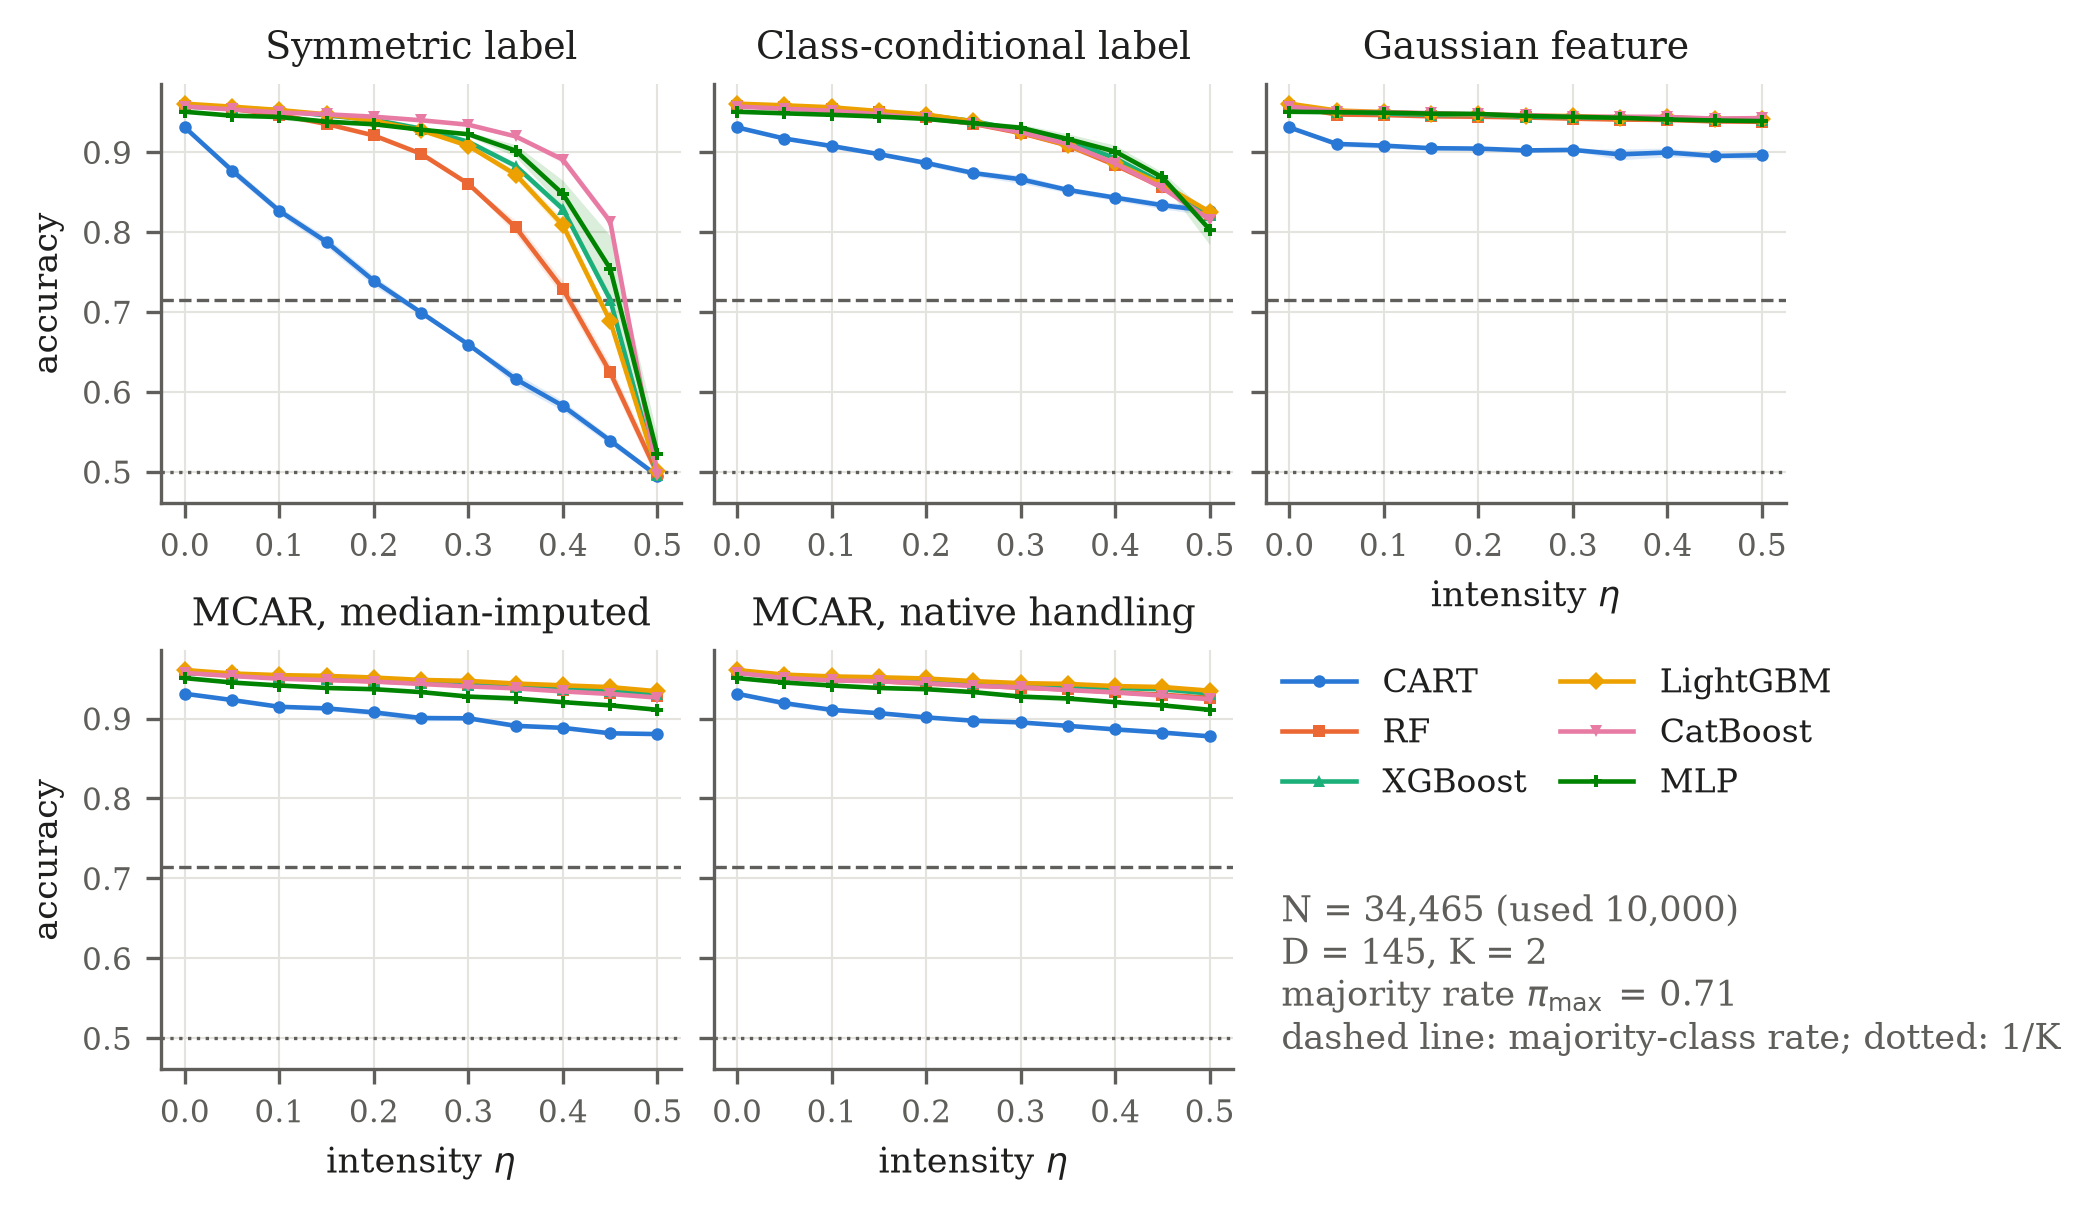
\includegraphics[width=\linewidth]{curves_nomao.png}
  \caption{nomao}\label{fig:atlas_nomao}
\end{subfigure}
\caption{Degradation atlas for business, marketing and web data (continued). Band: $\pm1$ sample SD across three seeds; dashed line: $\pi_{\max}$.}
\end{figure}

\begin{figure}[tbp]
\ContinuedFloat
\centering
\begin{subfigure}{\linewidth}
  \centering
  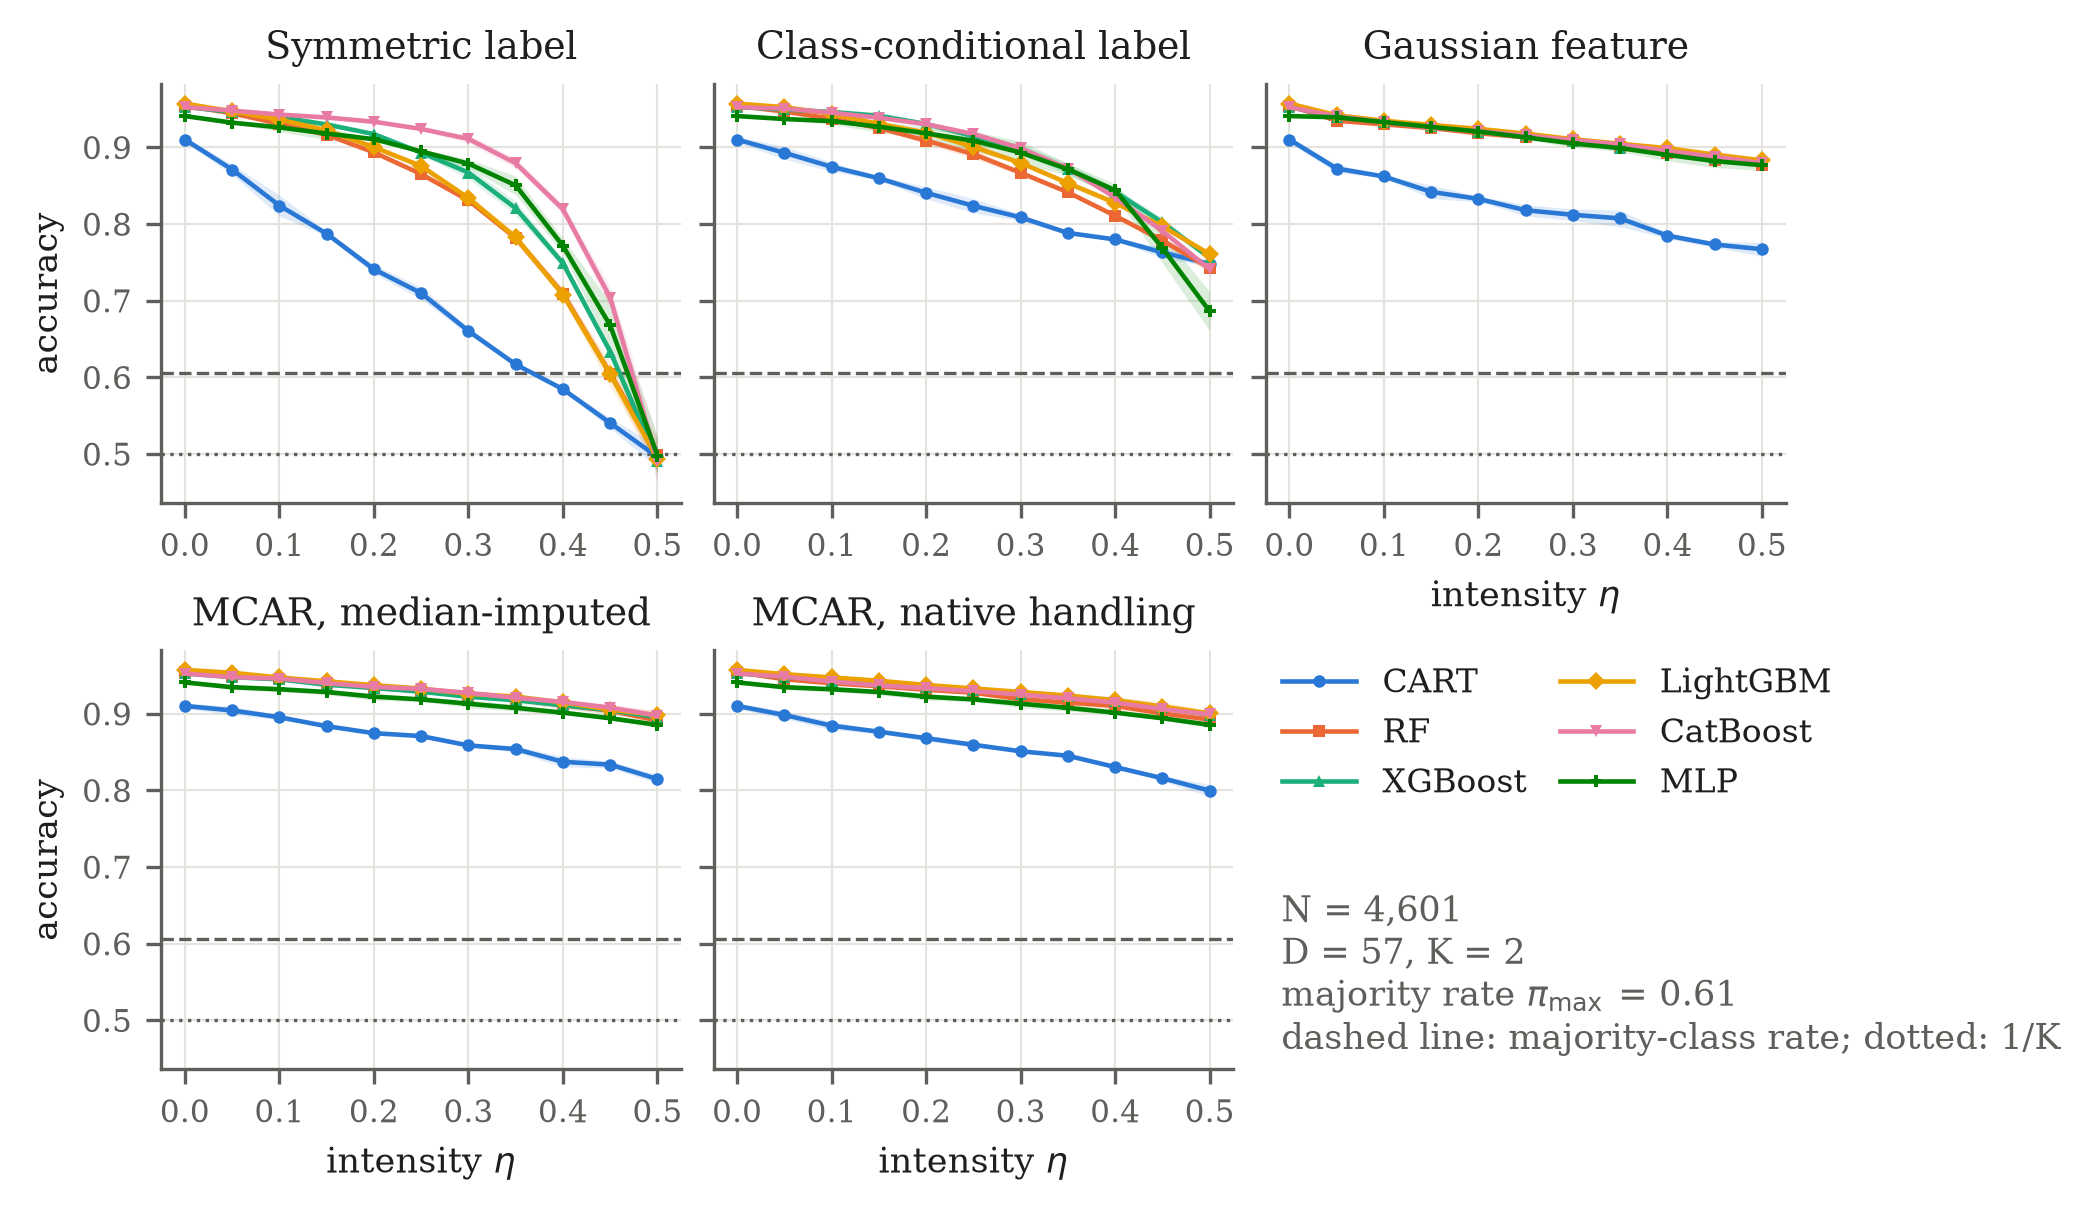
\includegraphics[width=\linewidth]{curves_spambase.png}
  \caption{spambase}\label{fig:atlas_spambase}
\end{subfigure}
\caption{Degradation atlas for business, marketing and web data (continued). Band: $\pm1$ sample SD across three seeds; dashed line: $\pi_{\max}$.}
\end{figure}

\begin{figure}[tbp]

\centering
\begin{subfigure}{\linewidth}
  \centering
  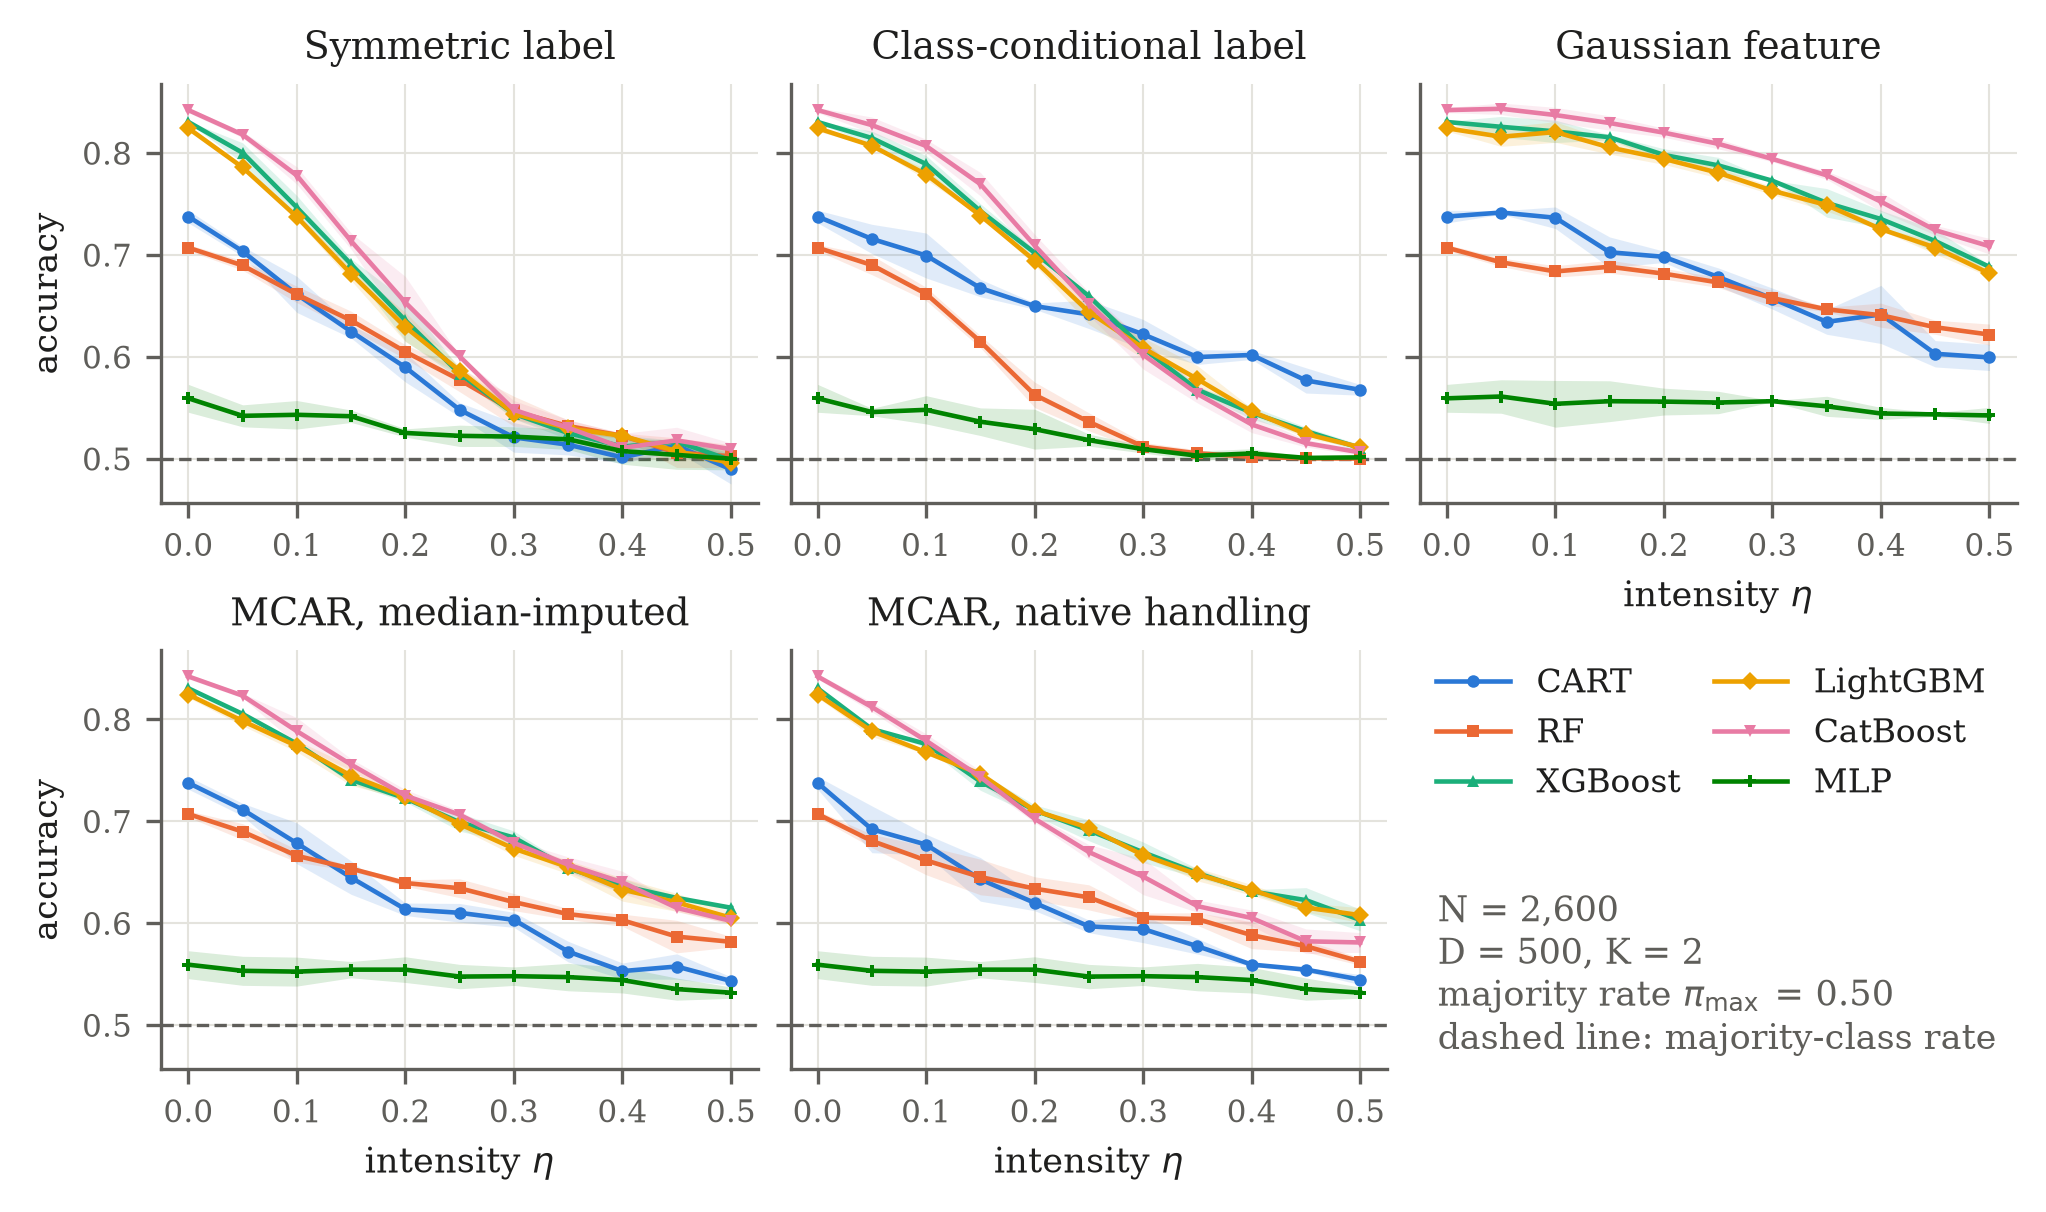
\includegraphics[width=\linewidth]{curves_madelon.png}
  \caption{madelon}\label{fig:atlas_madelon}
\end{subfigure}\\[4pt]
\begin{subfigure}{\linewidth}
  \centering
  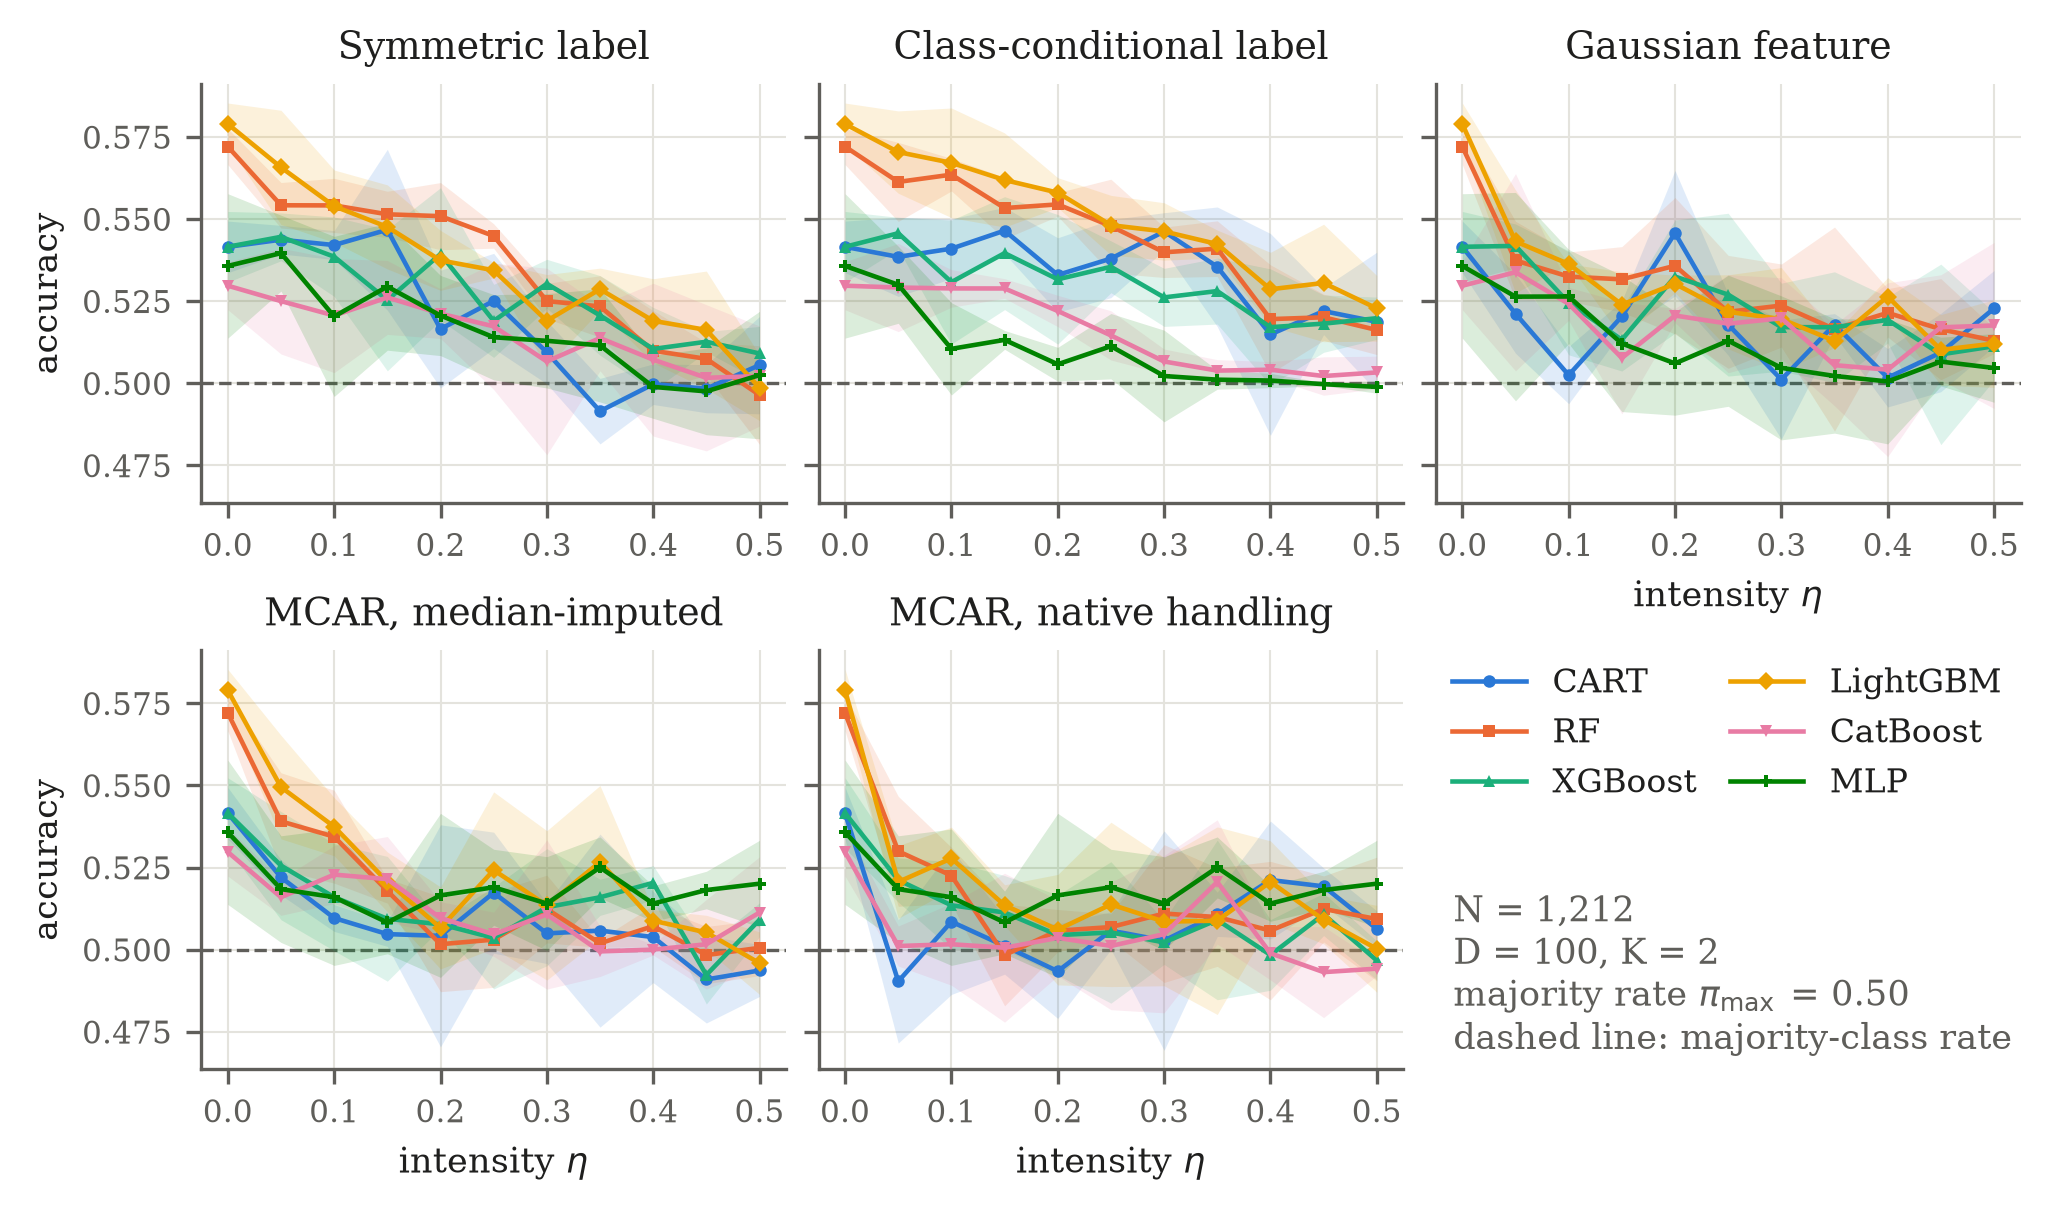
\includegraphics[width=\linewidth]{curves_hill_valley.png}
  \caption{hill\_valley}\label{fig:atlas_hill_valley}
\end{subfigure}
\caption{Degradation atlas for synthetic, game, speech and image-derived tasks. Median MRR of the group: $0.933$ (symmetric label noise), $0.910$ (class-conditional label noise), $0.936$ (Gaussian feature noise), $0.912$ (imputed masking) and $0.910$ (native masking); mean AUDC over its datasets and all five conditions from $0.586$ (CART) to $0.676$ (LightGBM). Band: $\pm1$ sample SD across three seeds; dashed line: $\pi_{\max}$.}
\label{fig:atlas_g4}
\end{figure}

\begin{figure}[tbp]
\ContinuedFloat
\centering
\begin{subfigure}{\linewidth}
  \centering
  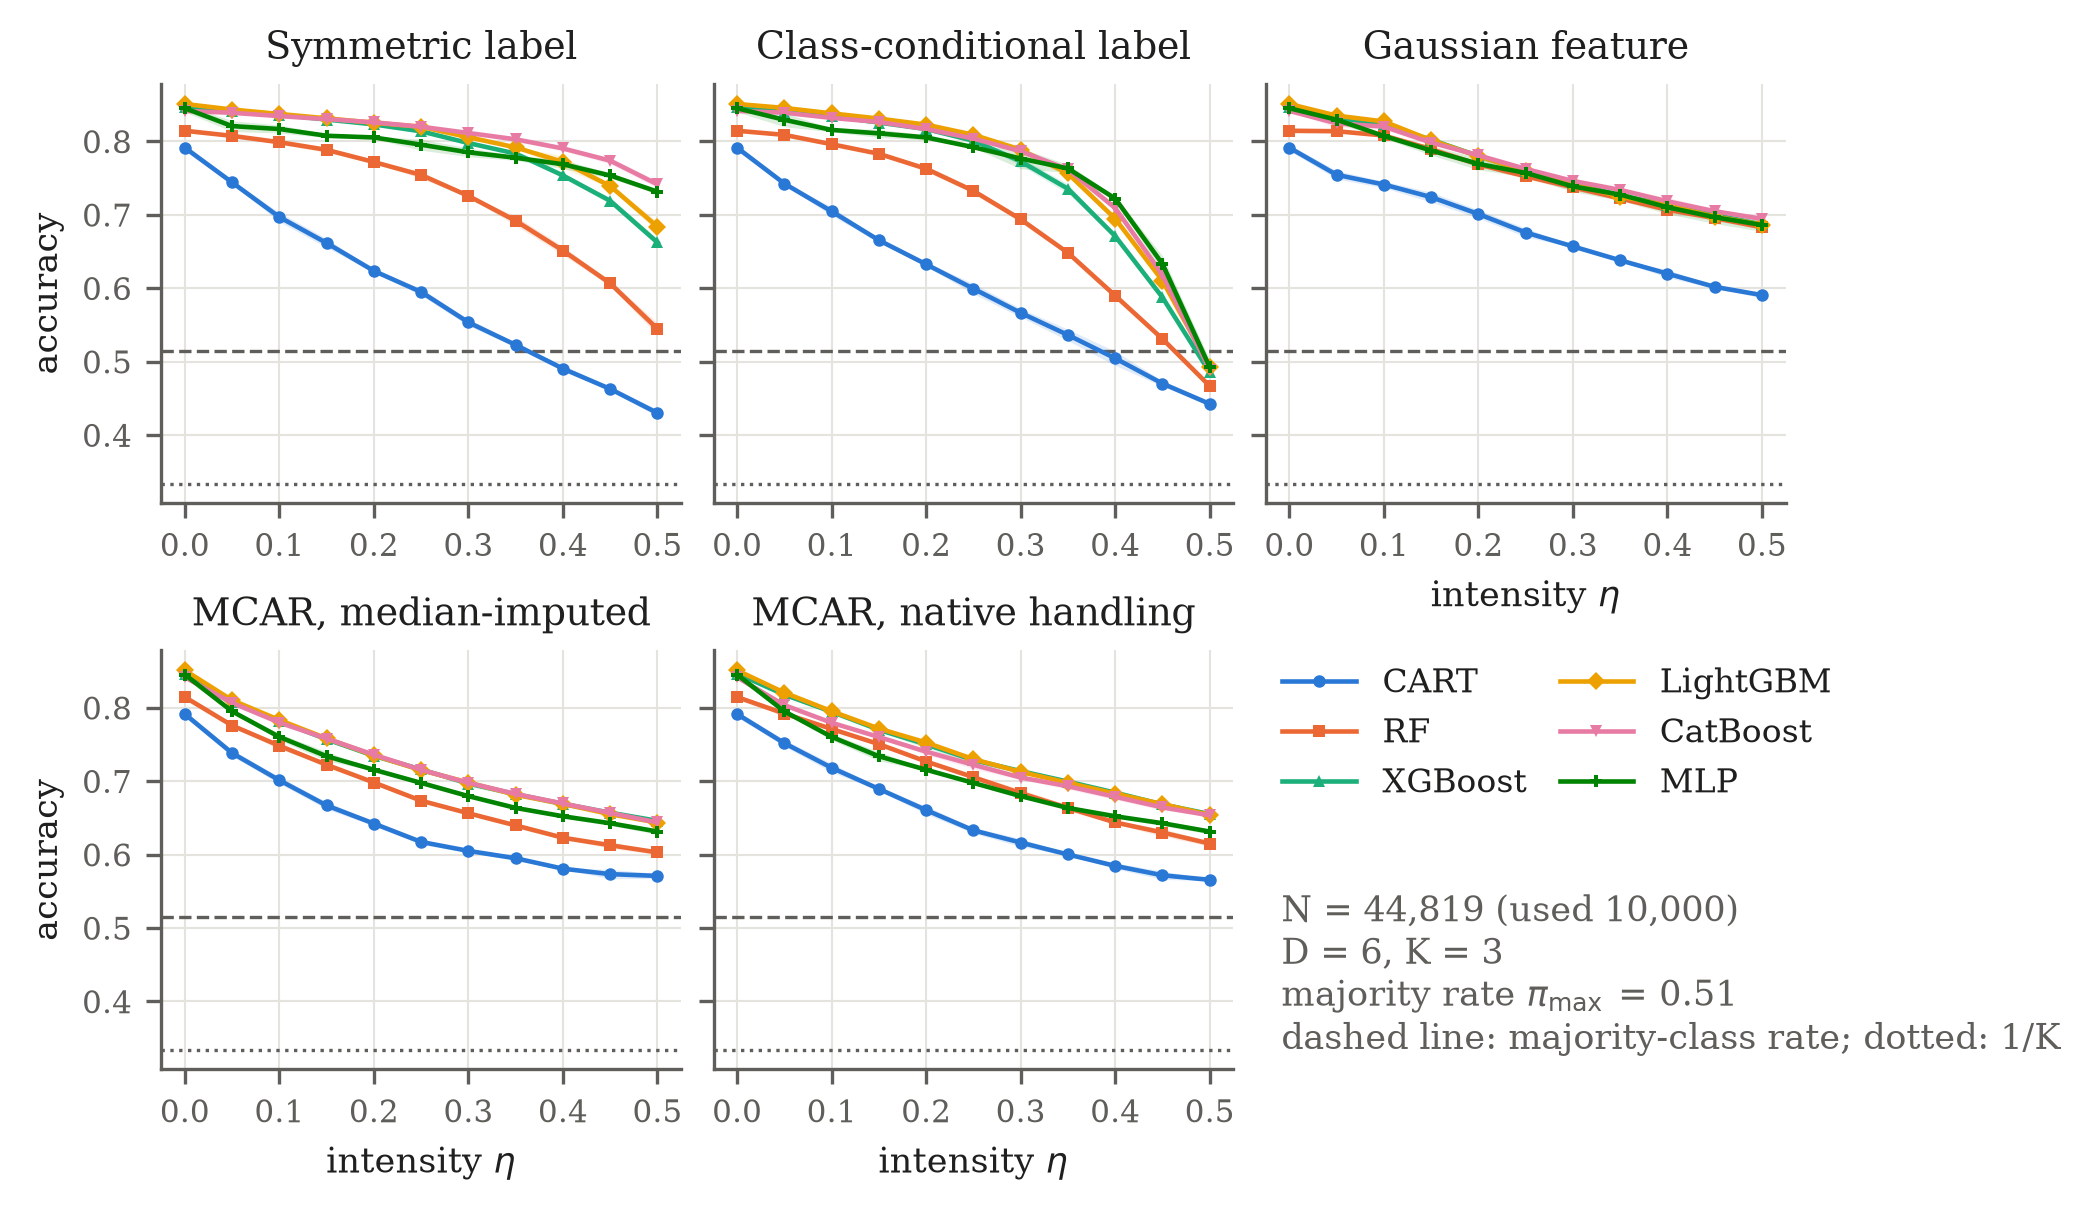
\includegraphics[width=\linewidth]{curves_jungle_chess.png}
  \caption{jungle\_chess}\label{fig:atlas_jungle_chess}
\end{subfigure}\\[4pt]
\begin{subfigure}{\linewidth}
  \centering
  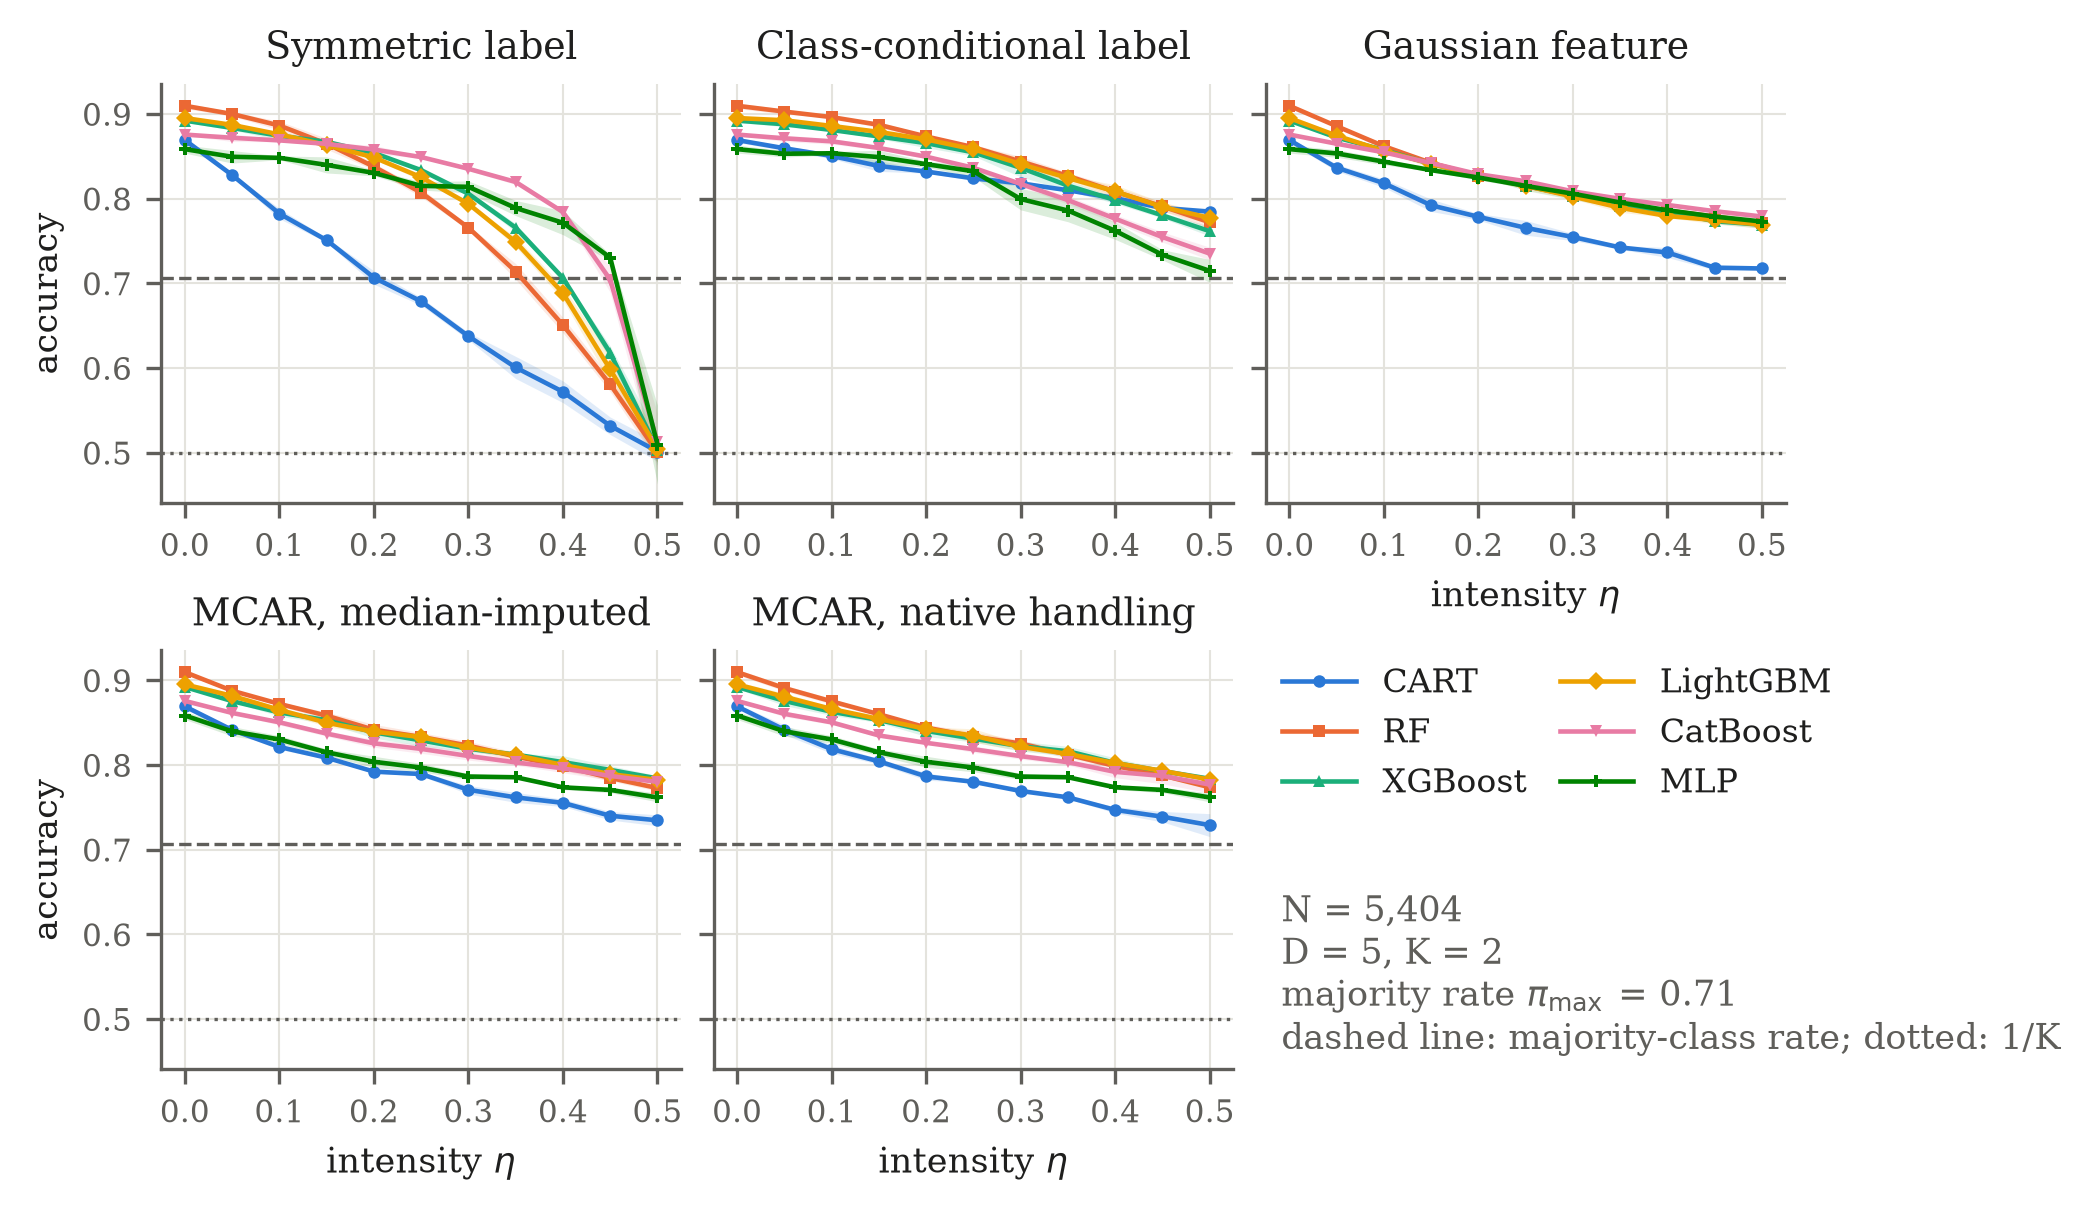
\includegraphics[width=\linewidth]{curves_phoneme.png}
  \caption{phoneme}\label{fig:atlas_phoneme}
\end{subfigure}
\caption{Degradation atlas for synthetic, game, speech and image-derived tasks (continued). Band: $\pm1$ sample SD across three seeds; dashed line: $\pi_{\max}$.}
\end{figure}

\begin{figure}[tbp]
\ContinuedFloat
\centering
\begin{subfigure}{\linewidth}
  \centering
  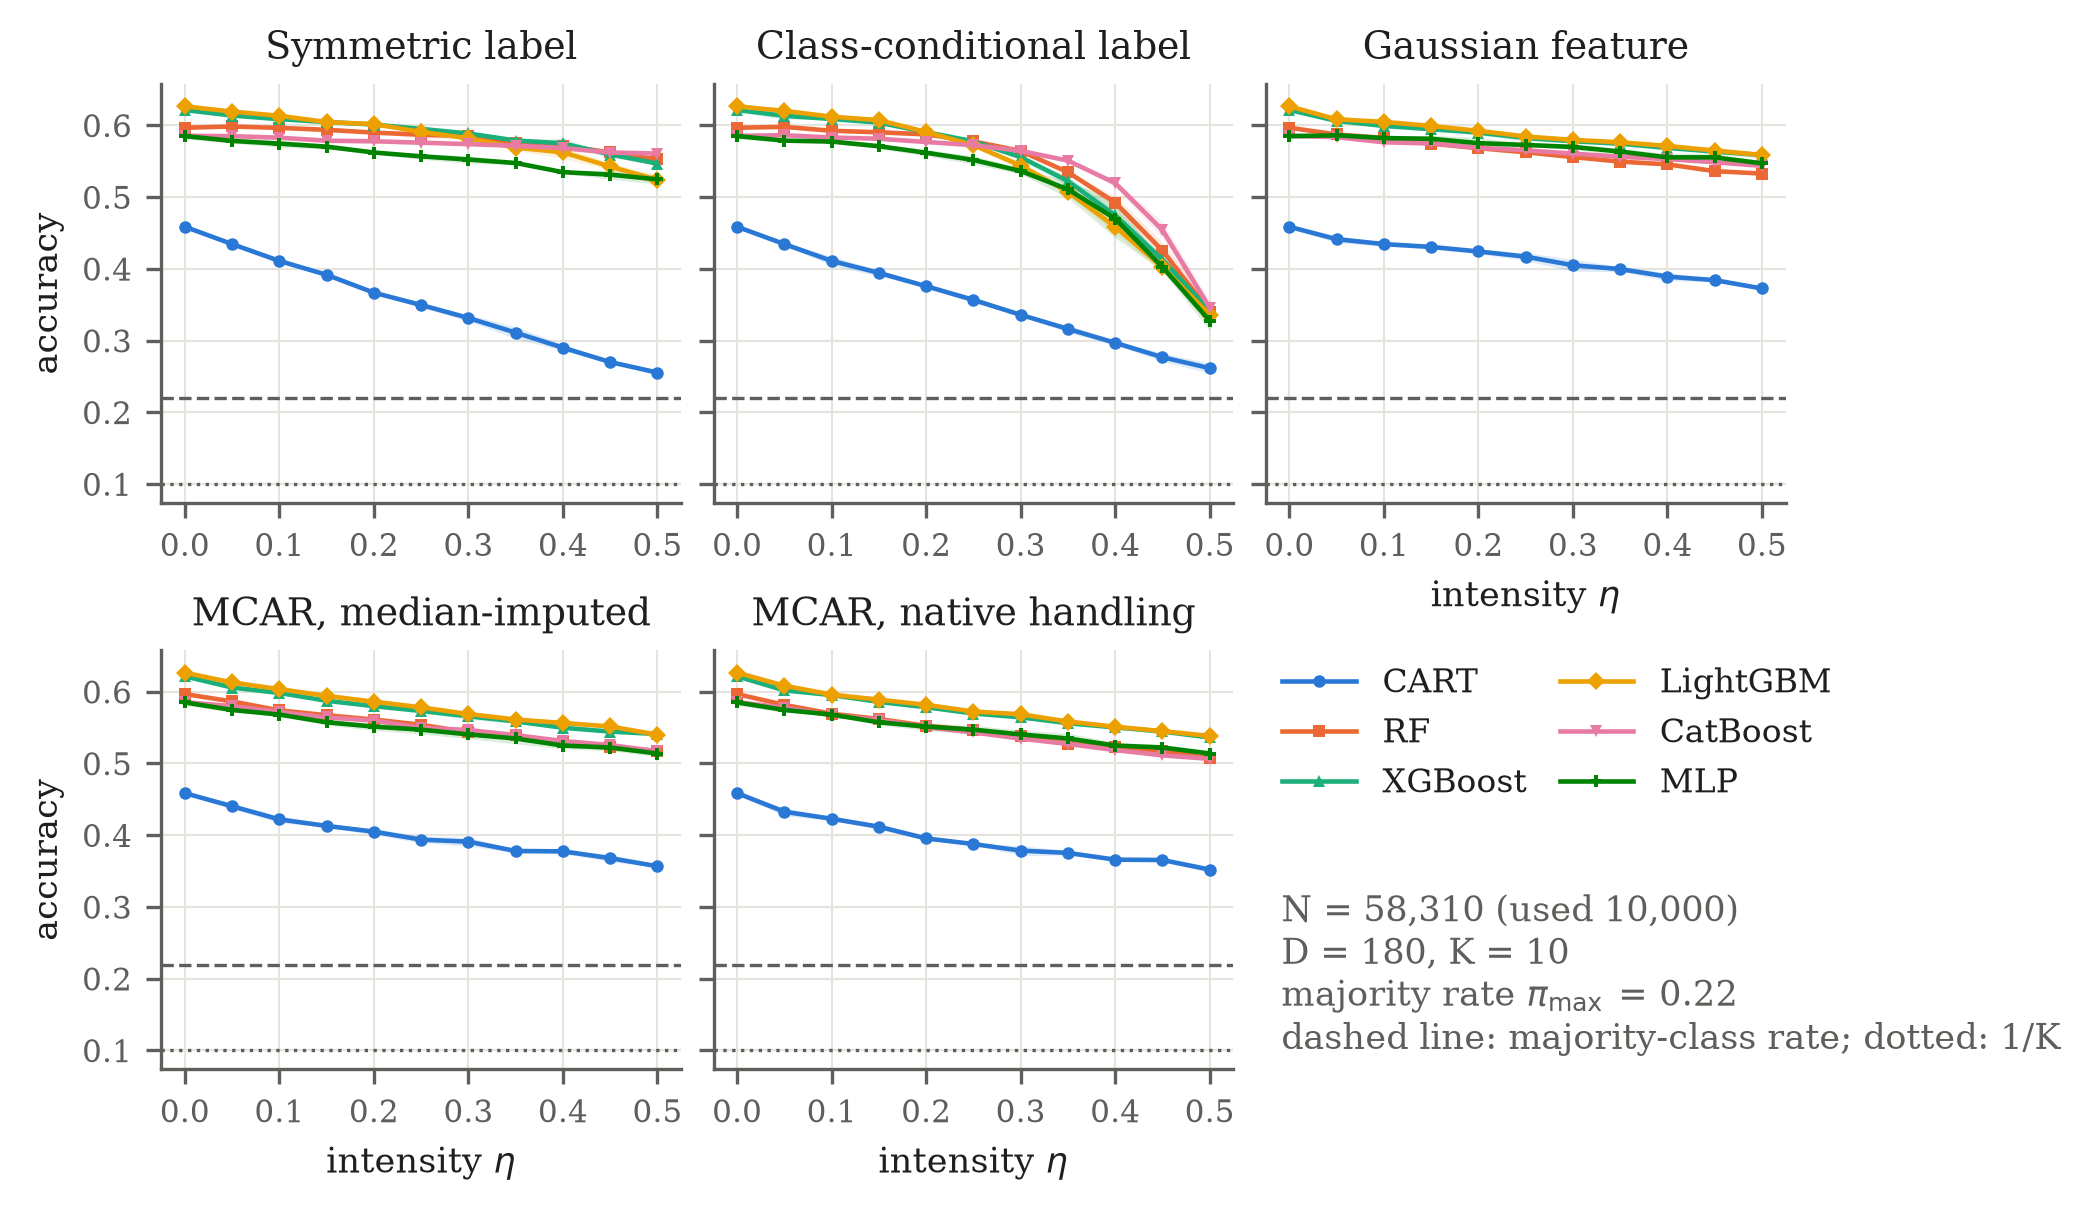
\includegraphics[width=\linewidth]{curves_volkert.png}
  \caption{volkert}\label{fig:atlas_volkert}
\end{subfigure}
\caption{Degradation atlas for synthetic, game, speech and image-derived tasks (continued). Band: $\pm1$ sample SD across three seeds; dashed line: $\pi_{\max}$.}
\end{figure}

\clearpage
%% ---- end inlined ../results/analysis/latex_primary/atlas_primary.tex ----

\clearpage
\section{Pairwise Wilcoxon tests}\label{sup:wilcoxon}
%% ---- begin inlined ../results/analysis/latex_primary/tab_wilcoxon.tex ----
{\scriptsize
\begin{longtable}{@{}lrrrl@{}}
\caption{Pairwise Wilcoxon signed-rank tests (Pratt zero handling) over the 20 datasets, with Holm adjustment over the 15 pairs of each block. $\dagger$ marks disagreement with the Nemenyi verdict.}\label{tab:wilcoxon}\\
\toprule
Pair & Median diff. & $p$ & $p_{\mathrm{Holm}}$ & Sig. \\
\midrule
\endfirsthead
\toprule
Pair & Median diff. & $p$ & $p_{\mathrm{Holm}}$ & Sig. \\
\midrule
\endhead
\multicolumn{5}{@{}l}{\textit{MRR, Symmetric label}} \\
CART--CatBoost & $-0.1534$ & $5.7\times10^{-6}$ & $6.9\times10^{-5}$ & yes \\
CART--LightGBM & $-0.1017$ & $3.6\times10^{-5}$ & $2.9\times10^{-4}$ & yes$\dagger$ \\
CART--MLP & $-0.1538$ & $1.9\times10^{-6}$ & $2.9\times10^{-5}$ & yes \\
CART--RF & $-0.1119$ & $5.7\times10^{-6}$ & $6.9\times10^{-5}$ & yes \\
CART--XGBoost & $-0.1186$ & $9.5\times10^{-6}$ & $9.5\times10^{-5}$ & yes \\
CatBoost--LightGBM & $+0.0430$ & $1.9\times10^{-6}$ & $2.9\times10^{-5}$ & yes \\
CatBoost--MLP & $+0.0078$ & 0.294 & 0.736 & no \\
CatBoost--RF & $+0.0304$ & $5.9\times10^{-4}$ & 0.004 & yes \\
CatBoost--XGBoost & $+0.0298$ & $1.9\times10^{-6}$ & $2.9\times10^{-5}$ & yes \\
LightGBM--MLP & $-0.0409$ & $1.3\times10^{-4}$ & $9.3\times10^{-4}$ & yes \\
LightGBM--RF & $-0.0104$ & 0.245 & 0.736 & no \\
LightGBM--XGBoost & $-0.0114$ & $1.9\times10^{-5}$ & $1.7\times10^{-4}$ & yes$\dagger$ \\
MLP--RF & $+0.0333$ & 0.004 & 0.018 & yes$\dagger$ \\
MLP--XGBoost & $+0.0207$ & 0.004 & 0.018 & yes$\dagger$ \\
RF--XGBoost & $-0.0090$ & 0.622 & 0.736 & no \\
\midrule
\multicolumn{5}{@{}l}{\textit{MRR, Class-cond.\ label}} \\
CART--CatBoost & $-0.0018$ & 0.177 & 1.000 & no \\
CART--LightGBM & $+0.0010$ & 0.294 & 1.000 & no \\
CART--MLP & $-0.0212$ & 0.058 & 0.641 & no \\
CART--RF & $+0.0077$ & 0.596 & 1.000 & no \\
CART--XGBoost & $+0.0016$ & 0.231 & 1.000 & no \\
CatBoost--LightGBM & $+0.0019$ & 0.058 & 0.641 & no \\
CatBoost--MLP & $-0.0010$ & 0.812 & 1.000 & no \\
CatBoost--RF & $+0.0100$ & 0.002 & 0.025 & yes$\dagger$ \\
CatBoost--XGBoost & $-0.0011$ & 0.571 & 1.000 & no \\
LightGBM--MLP & $-0.0060$ & 0.004 & 0.059 & no \\
LightGBM--RF & $+0.0011$ & 0.812 & 1.000 & no \\
LightGBM--XGBoost & $-0.0039$ & 0.030 & 0.384 & no \\
MLP--RF & $+0.0099$ & 0.036 & 0.435 & no$\dagger$ \\
MLP--XGBoost & $+0.0032$ & 0.076 & 0.641 & no \\
RF--XGBoost & $-0.0062$ & 0.070 & 0.641 & no \\
\midrule
\multicolumn{5}{@{}l}{\textit{MRR, Gaussian feature}} \\
CART--CatBoost & $-0.0427$ & $1.9\times10^{-6}$ & $2.9\times10^{-5}$ & yes \\
CART--LightGBM & $-0.0229$ & $3.9\times10^{-4}$ & 0.004 & yes$\dagger$ \\
CART--MLP & $-0.0420$ & $9.5\times10^{-6}$ & $1.2\times10^{-4}$ & yes \\
CART--RF & $-0.0259$ & $1.0\times10^{-4}$ & 0.001 & yes \\
CART--XGBoost & $-0.0320$ & $5.7\times10^{-6}$ & $8.0\times10^{-5}$ & yes \\
CatBoost--LightGBM & $+0.0047$ & 0.002 & 0.016 & yes \\
CatBoost--MLP & $-0.0069$ & 0.123 & 0.369 & no \\
CatBoost--RF & $+0.0039$ & 0.015 & 0.092 & no \\
CatBoost--XGBoost & $+0.0048$ & $7.1\times10^{-4}$ & 0.007 & yes$\dagger$ \\
LightGBM--MLP & $-0.0099$ & 0.004 & 0.034 & yes \\
LightGBM--RF & $-0.0032$ & 0.189 & 0.379 & no \\
LightGBM--XGBoost & $-0.0013$ & 0.005 & 0.034 & yes$\dagger$ \\
MLP--RF & $+0.0111$ & 0.016 & 0.092 & no \\
MLP--XGBoost & $+0.0060$ & 0.026 & 0.105 & no \\
RF--XGBoost & $-0.0009$ & 0.467 & 0.467 & no \\
\midrule
\multicolumn{5}{@{}l}{\textit{MRR, MCAR, imputed}} \\
CART--CatBoost & $-0.0317$ & $1.9\times10^{-6}$ & $2.9\times10^{-5}$ & yes \\
CART--LightGBM & $-0.0208$ & $1.7\times10^{-4}$ & 0.002 & yes \\
CART--MLP & $-0.0241$ & $5.7\times10^{-6}$ & $7.4\times10^{-5}$ & yes \\
CART--RF & $-0.0187$ & $2.1\times10^{-4}$ & 0.002 & yes \\
CART--XGBoost & $-0.0258$ & $1.9\times10^{-6}$ & $2.9\times10^{-5}$ & yes \\
CatBoost--LightGBM & $+0.0024$ & 0.070 & 0.696 & no \\
CatBoost--MLP & $+0.0012$ & 0.216 & 1.000 & no \\
CatBoost--RF & $+0.0019$ & 0.165 & 1.000 & no \\
CatBoost--XGBoost & $+0.0016$ & 0.133 & 1.000 & no \\
LightGBM--MLP & $-0.0018$ & 0.546 & 1.000 & no \\
LightGBM--RF & $+0.0009$ & 0.648 & 1.000 & no \\
LightGBM--XGBoost & $-0.0009$ & 0.114 & 1.000 & no \\
MLP--RF & $+0.0015$ & 0.409 & 1.000 & no \\
MLP--XGBoost & $+0.0009$ & 0.756 & 1.000 & no \\
RF--XGBoost & $-0.0005$ & 0.452 & 1.000 & no \\
\midrule
\multicolumn{5}{@{}l}{\textit{MRR, MCAR, native}} \\
CART--CatBoost & $-0.0312$ & $4.8\times10^{-5}$ & $6.2\times10^{-4}$ & yes \\
CART--LightGBM & $-0.0301$ & $2.1\times10^{-4}$ & 0.003 & yes \\
CART--MLP & $-0.0250$ & $3.8\times10^{-6}$ & $5.3\times10^{-5}$ & yes \\
CART--RF & $-0.0231$ & $2.6\times10^{-4}$ & 0.003 & yes \\
CART--XGBoost & $-0.0326$ & $1.9\times10^{-6}$ & $2.9\times10^{-5}$ & yes \\
CatBoost--LightGBM & $-0.0007$ & 0.927 & 1.000 & no \\
CatBoost--MLP & $-0.0004$ & 0.648 & 1.000 & no \\
CatBoost--RF & $+0.0019$ & 0.294 & 1.000 & no \\
CatBoost--XGBoost & $-0.0005$ & 0.756 & 1.000 & no \\
LightGBM--MLP & $-0.0006$ & 0.546 & 1.000 & no \\
LightGBM--RF & $+0.0021$ & 0.090 & 0.718 & no \\
LightGBM--XGBoost & $-0.0016$ & 0.070 & 0.626 & no \\
MLP--RF & $+0.0018$ & 0.312 & 1.000 & no \\
MLP--XGBoost & $+0.0001$ & 0.985 & 1.000 & no \\
RF--XGBoost & $-0.0038$ & 0.021 & 0.215 & no \\
\midrule
\multicolumn{5}{@{}l}{\textit{AUDC, Symmetric label}} \\
CART--CatBoost & $-0.1707$ & $3.8\times10^{-6}$ & $4.6\times10^{-5}$ & yes \\
CART--LightGBM & $-0.1375$ & $1.9\times10^{-6}$ & $2.9\times10^{-5}$ & yes \\
CART--MLP & $-0.1490$ & $9.5\times10^{-6}$ & $1.0\times10^{-4}$ & yes \\
CART--RF & $-0.1312$ & $1.9\times10^{-6}$ & $2.9\times10^{-5}$ & yes \\
CART--XGBoost & $-0.1412$ & $1.9\times10^{-6}$ & $2.9\times10^{-5}$ & yes \\
CatBoost--LightGBM & $+0.0266$ & 0.019 & 0.192 & no \\
CatBoost--MLP & $+0.0182$ & 0.058 & 0.350 & no \\
CatBoost--RF & $+0.0231$ & 0.021 & 0.193 & no \\
CatBoost--XGBoost & $+0.0214$ & 0.033 & 0.262 & no \\
LightGBM--MLP & $-0.0118$ & 0.898 & 1.000 & no \\
LightGBM--RF & $+0.0029$ & 0.452 & 1.000 & no \\
LightGBM--XGBoost & $-0.0054$ & 0.044 & 0.308 & no \\
MLP--RF & $+0.0002$ & 0.596 & 1.000 & no \\
MLP--XGBoost & $+0.0031$ & 0.927 & 1.000 & no \\
RF--XGBoost & $-0.0087$ & 0.261 & 1.000 & no \\
\midrule
\multicolumn{5}{@{}l}{\textit{AUDC, Class-cond.\ label}} \\
CART--CatBoost & $-0.0405$ & $1.3\times10^{-5}$ & $1.7\times10^{-4}$ & yes \\
CART--LightGBM & $-0.0460$ & $1.9\times10^{-6}$ & $2.9\times10^{-5}$ & yes \\
CART--MLP & $-0.0301$ & 0.003 & 0.025 & yes$\dagger$ \\
CART--RF & $-0.0380$ & $2.6\times10^{-4}$ & 0.003 & yes \\
CART--XGBoost & $-0.0463$ & $3.8\times10^{-6}$ & $5.3\times10^{-5}$ & yes \\
CatBoost--LightGBM & $-0.0010$ & 0.368 & 1.000 & no \\
CatBoost--MLP & $+0.0121$ & 0.001 & 0.010 & yes$\dagger$ \\
CatBoost--RF & $+0.0027$ & 0.475 & 1.000 & no \\
CatBoost--XGBoost & $-0.0019$ & 0.105 & 0.422 & no \\
LightGBM--MLP & $+0.0136$ & $3.9\times10^{-4}$ & 0.004 & yes \\
LightGBM--RF & $+0.0046$ & 0.058 & 0.350 & no \\
LightGBM--XGBoost & $-0.0000$ & 0.985 & 1.000 & no \\
MLP--RF & $-0.0067$ & 0.058 & 0.350 & no \\
MLP--XGBoost & $-0.0157$ & 0.001 & 0.011 & yes \\
RF--XGBoost & $-0.0032$ & 0.048 & 0.339 & no \\
\midrule
\multicolumn{5}{@{}l}{\textit{AUDC, Gaussian feature}} \\
CART--CatBoost & $-0.0780$ & $1.9\times10^{-6}$ & $2.9\times10^{-5}$ & yes \\
CART--LightGBM & $-0.0785$ & $3.8\times10^{-6}$ & $5.3\times10^{-5}$ & yes \\
CART--MLP & $-0.0635$ & $8.5\times10^{-4}$ & 0.009 & yes$\dagger$ \\
CART--RF & $-0.0679$ & $9.5\times10^{-6}$ & $1.1\times10^{-4}$ & yes \\
CART--XGBoost & $-0.0772$ & $3.8\times10^{-6}$ & $5.3\times10^{-5}$ & yes \\
CatBoost--LightGBM & $-0.0008$ & 0.165 & 0.660 & no \\
CatBoost--MLP & $+0.0030$ & 0.019 & 0.115 & no$\dagger$ \\
CatBoost--RF & $+0.0020$ & 0.475 & 0.950 & no \\
CatBoost--XGBoost & $+0.0008$ & 0.812 & 0.950 & no \\
LightGBM--MLP & $+0.0057$ & $3.2\times10^{-4}$ & 0.004 & yes \\
LightGBM--RF & $+0.0033$ & 0.001 & 0.010 & yes$\dagger$ \\
LightGBM--XGBoost & $+0.0009$ & 0.003 & 0.019 & yes$\dagger$ \\
MLP--RF & $-0.0019$ & 0.165 & 0.660 & no \\
MLP--XGBoost & $-0.0050$ & 0.001 & 0.009 & yes$\dagger$ \\
RF--XGBoost & $-0.0019$ & 0.076 & 0.379 & no \\
\midrule
\multicolumn{5}{@{}l}{\textit{AUDC, MCAR, imputed}} \\
CART--CatBoost & $-0.0600$ & $1.9\times10^{-6}$ & $2.9\times10^{-5}$ & yes \\
CART--LightGBM & $-0.0625$ & $1.9\times10^{-6}$ & $2.9\times10^{-5}$ & yes \\
CART--MLP & $-0.0389$ & $3.9\times10^{-4}$ & 0.004 & yes$\dagger$ \\
CART--RF & $-0.0550$ & $1.9\times10^{-6}$ & $2.9\times10^{-5}$ & yes \\
CART--XGBoost & $-0.0589$ & $1.9\times10^{-6}$ & $2.9\times10^{-5}$ & yes \\
CatBoost--LightGBM & $-0.0056$ & 0.007 & 0.029 & yes$\dagger$ \\
CatBoost--MLP & $+0.0138$ & 0.001 & 0.007 & yes$\dagger$ \\
CatBoost--RF & $-0.0010$ & 0.430 & 0.624 & no \\
CatBoost--XGBoost & $-0.0022$ & 0.011 & 0.032 & yes$\dagger$ \\
LightGBM--MLP & $+0.0182$ & $1.9\times10^{-6}$ & $2.9\times10^{-5}$ & yes \\
LightGBM--RF & $+0.0037$ & $5.9\times10^{-4}$ & 0.005 & yes$\dagger$ \\
LightGBM--XGBoost & $+0.0022$ & 0.006 & 0.028 & yes$\dagger$ \\
MLP--RF & $-0.0118$ & 0.001 & 0.007 & yes \\
MLP--XGBoost & $-0.0168$ & $6.3\times10^{-5}$ & $6.3\times10^{-4}$ & yes \\
RF--XGBoost & $-0.0005$ & 0.312 & 0.624 & no \\
\midrule
\multicolumn{5}{@{}l}{\textit{AUDC, MCAR, native}} \\
CART--CatBoost & $-0.0533$ & $3.8\times10^{-6}$ & $4.6\times10^{-5}$ & yes \\
CART--LightGBM & $-0.0740$ & $1.9\times10^{-6}$ & $2.9\times10^{-5}$ & yes \\
CART--MLP & $-0.0404$ & $2.6\times10^{-4}$ & 0.001 & yes$\dagger$ \\
CART--RF & $-0.0591$ & $1.9\times10^{-6}$ & $2.9\times10^{-5}$ & yes \\
CART--XGBoost & $-0.0682$ & $1.9\times10^{-6}$ & $2.9\times10^{-5}$ & yes \\
CatBoost--LightGBM & $-0.0107$ & $3.8\times10^{-6}$ & $4.6\times10^{-5}$ & yes \\
CatBoost--MLP & $+0.0104$ & 0.012 & 0.024 & yes$\dagger$ \\
CatBoost--RF & $-0.0007$ & 0.388 & 0.388 & no \\
CatBoost--XGBoost & $-0.0085$ & $3.8\times10^{-6}$ & $4.6\times10^{-5}$ & yes$\dagger$ \\
LightGBM--MLP & $+0.0245$ & $5.7\times10^{-6}$ & $5.1\times10^{-5}$ & yes \\
LightGBM--RF & $+0.0067$ & $1.9\times10^{-5}$ & $1.5\times10^{-4}$ & yes \\
LightGBM--XGBoost & $+0.0016$ & $1.0\times10^{-4}$ & $7.3\times10^{-4}$ & yes$\dagger$ \\
MLP--RF & $-0.0090$ & 0.002 & 0.006 & yes$\dagger$ \\
MLP--XGBoost & $-0.0230$ & $1.0\times10^{-4}$ & $7.3\times10^{-4}$ & yes \\
RF--XGBoost & $-0.0043$ & $5.9\times10^{-4}$ & 0.002 & yes$\dagger$ \\
\bottomrule
\end{longtable}
}
%% ---- end inlined ../results/analysis/latex_primary/tab_wilcoxon.tex ----

\clearpage
\section{Sensitivity runs and additional statistics}\label{sup:sens}
Four additions to the analysis in the article, none of which enters the confirmatory family. All tables are generated by \texttt{experiments/analyze\_sensitivity.py}.

\paragraph{TabICL settings.} The main TabICL run uses four estimators and caps the in-context set at 3{,}000 rows. We repeated Protocol~B for seed 42 on six datasets with the library defaults (eight estimators, no cap). Mean clean accuracy changes from $0.935$ to $0.938$ (largest per-dataset change $0.013$). The MRR mean rank of TabICL among the seven models is identical in both runs under all four operators, whereas its balanced-AUDC rank improves or stays equal under every operator, most under MNAR masking, where it moves from 3.67 to 2.83 (position fifth to first). The leader of the seven changes in one of the eight score--operator cells. With six datasets this is a check on the direction of the effect, not an estimate of its size.

\paragraph{Compound corruption.} Label noise or Gaussian noise was applied together with MCAR missingness at the same intensity $\eta$ under Protocol~A, on six datasets, seeds 42, 43 and 44 and the six classical families. The compound loss of accuracy is smaller than the sum of the two single-operator losses (median difference $-0.019$ for label noise with MCAR and $-0.002$ for Gaussian noise with MCAR; sub-additive in at least 67\% of the dataset--model pairs). The mean-rank order under the compound operator follows the label or Gaussian component (MRR $\tau\ge0.96$) and agrees much less with the MCAR component ($\tau$ as low as 0.28 for MRR, 0.28 over both scores). With six models and six datasets these correlations are coarse.

\subsection{Continuous-only Gaussian noise}
The Gaussian condition of every analysis, in the main article and in this supplement, restricts Gaussian noise to the continuous attributes and leaves nominal attributes clean (the principal Gaussian experiment). It differs from the all-column variant on the six datasets with nominal attributes only; the principal-versus-all-column table of the main article compares the two. The TabICL comparison and the compound-corruption runs are the exception: they were run with the all-column operator and are labelled as such where they are reported.

\paragraph{Bayesian signed-rank test.} For each confirmatory condition we compared the best and the second-best family on balanced AUDC with the Bayesian signed-rank test of Benavoli et al.~\cite{benavoli2016should} (Dirichlet-process prior of strength 0.5 at zero, ROPE $\pm0.01$, 20{,}000 posterior samples). The best family is the winning decision in at most 28\% of the samples under any condition; the practical-equivalence region has the highest posterior probability in five of the five conditions. The leading families are therefore separated in rank, as the Friedman tests show, but not in the size of the difference: the median gap between the first two families is below one percentage point of balanced AUDC under every condition.

\paragraph{Bootstrap intervals for the TabICL gap.} Table~\ref{tab:sens_gap} gives the median difference in MRR between TabICL and the best classical family with a bootstrap 95\% interval over datasets; every interval lies below zero.

%% ---- begin inlined ../results/analysis/revision/tab_sensitivity_extra.tex ----
\begin{table}[t]
\centering
\footnotesize
\caption{TabICL settings check (seed 42, Protocol~B, 6 datasets): main run (4 estimators, in-context set capped at 3,000 rows) against default settings (8 estimators, no cap). Mean rank of TabICL among the seven models and, in parentheses, its position.}
\label{tab:sens_settings}
\begin{tabular}{@{}llrrrr@{}}
\toprule
 & & \multicolumn{2}{c}{MRR} & \multicolumn{2}{c}{AUDC$_{\mathrm{bal}}$} \\
\cmidrule(lr){3-4}\cmidrule(lr){5-6}
Operator & & Main & Default & Main & Default \\
\midrule
Gaussian & & 6.83 (7) & 6.83 (7) & 5.00 (6) & 5.00 (6) \\
MCAR & & 5.33 (6) & 5.33 (6) & 2.33 (1) & 2.00 (1) \\
MAR & & 5.17 (6) & 5.17 (6) & 1.83 (1) & 1.67 (1) \\
MNAR & & 5.17 (7) & 5.17 (7) & 3.67 (5) & 2.83 (1) \\
\midrule
Clean accuracy & & \multicolumn{2}{c}{0.935} & \multicolumn{2}{c}{0.938} \\
\bottomrule
\end{tabular}
\end{table}

\begin{table}[t]
\centering
\footnotesize
\caption{Compound corruption under Protocol~A (6 datasets, seeds 42, 43, 44, six classical families). $\tau$: Kendall correlation between the mean-rank vector under the compound operator and under each component alone. Additivity: median over dataset--model pairs of the compound AUDC loss (clean value minus AUDC) minus the sum of the two single-operator losses; negative values are sub-additive.}
\label{tab:sens_compound}
\begin{tabular}{@{}lllrrr@{}}
\toprule
Compound & Score & Component & $\tau$ & Additivity & Sub-additive \\
\midrule
Label noise + MCAR & MRR & label noise & 0.96 & $-0.019$ & 97\% \\
 & MRR & MCAR & 0.28 &  &  \\
 & AUDC$_{\mathrm{bal}}$ & label noise & 0.50 &  &  \\
 & AUDC$_{\mathrm{bal}}$ & MCAR & 0.36 &  &  \\
\midrule
Gaussian + MCAR & MRR & Gaussian & 0.97 & $-0.002$ & 67\% \\
 & MRR & MCAR & 0.41 &  &  \\
 & AUDC$_{\mathrm{bal}}$ & Gaussian & 1.00 &  &  \\
 & AUDC$_{\mathrm{bal}}$ & MCAR & 0.87 &  &  \\
\bottomrule
\end{tabular}
\end{table}

\begin{table}[t]
\centering
\footnotesize
\caption{Bayesian signed-rank test (ROPE $\pm0.01$ on balanced AUDC) between the best and the second-best family under each confirmatory condition: posterior probability that the best family is better (right), practically equivalent (ROPE) or worse (left), and the share of posterior samples in which the best family wins the decision.}
\label{tab:sens_bayes}
\begin{tabular}{@{}llrrrr@{}}
\toprule
Condition & Best / second & $P(\mathrm{best})$ & $P(\mathrm{ROPE})$ & $P(\mathrm{second})$ & Wins \\
\midrule
Symmetric label & CatBoost / XGBoost & 0.31 & 0.36 & 0.33 & 0.28 \\
Class-conditional & LightGBM / XGBoost & 0.16 & 0.83 & 0.01 & 0.00 \\
Gaussian & LightGBM / XGBoost & 0.10 & 0.90 & 0.00 & 0.00 \\
MCAR (imputed) & LightGBM / XGBoost & 0.20 & 0.80 & 0.00 & 0.01 \\
MCAR (native) & LightGBM / XGBoost & 0.12 & 0.88 & 0.00 & 0.00 \\
\bottomrule
\end{tabular}
\end{table}

\begin{table}[t]
\centering
\footnotesize
\caption{Median MRR difference between TabICL and the best classical family per dataset{,} with a bootstrap 95\% interval over datasets (10{,}000 resamples).}
\label{tab:sens_gap}
\begin{tabular}{@{}lrr@{}}
\toprule
Operator & Median & 95\% interval \\
\midrule
Gaussian & $-0.093$ & $[-0.193,\,-0.046]$ \\
MCAR & $-0.021$ & $[-0.044,\,-0.011]$ \\
MAR & $-0.019$ & $[-0.039,\,-0.006]$ \\
MNAR & $-0.023$ & $[-0.046,\,-0.010]$ \\
\bottomrule
\end{tabular}
\end{table}
%% ---- end inlined ../results/analysis/revision/tab_sensitivity_extra.tex ----

\clearpage
\section{Data cleaning rules and the pol class ordering}\label{sup:cleaning}

\paragraph{Cleaning rules and row counts.} The primary benchmark uses every upload unchanged, apart from the loader's encoding of categorical attributes, median imputation of any stored missing values and, for datasets above 10{,}000 rows, a fixed stratified subsample of 10{,}000 rows (seed 42). Cleaning is applied only to the artifact-sensitivity copies of Section~\ref{sup:sens} and the main article, by three rules that are kept apart: \emph{R1, duplicate removal}: of several rows with an identical feature vector and identical label, the first is kept and the rest are removed; \emph{R2, conflicting-duplicate removal}: when identical feature vectors carry more than one label, \emph{all} rows of that vector are removed, since no label can be kept without choice; \emph{R3, sentinel rows}: rows in which every feature equals $-999$ are removed. R1 and R2 are applied to spambase only; R3 to MiniBooNE only; for churn the identifier column \texttt{phone\_number} is dropped and no row is removed. Table~\ref{tab:cleaning_counts} gives the counts, computed by \texttt{experiments/dataset\_cleaning\_counts.py}. In spambase, 391 duplicate rows (R1) and 6 rows forming 3 conflicting feature vectors (R2) are removed, leaving 4{,}204 of 4{,}601 rows; in MiniBooNE all 468 sentinel rows are also conflicting duplicates, leaving 129{,}596 of 130{,}064.

%% ---- begin inlined ../results/analysis/revision/tab_cleaning_counts.tex ----
\begin{table}[htbp]
\centering\small
\caption{Rows before and after each cleaning rule, for the datasets on which at least one rule applies (the other 12 datasets are unaffected). R1 and R2 act on feature vectors, R3 on sentinel rows. Only the cleaned copies of spambase (R1 and R2), churn (identifier column) and MiniBooNE (R3) enter the artifact analysis; the other rows are reported for transparency.}\label{tab:cleaning_counts}
\begin{tabular}{@{}lrrrrrr@{}}
\toprule
Dataset & Rows & R1 duplicates & R2 conflicting & After R1+R2 & R3 sentinel & After R3 \\
\midrule
phoneme & 5{,}404 & 9 & 0 & 5{,}395 & 0 & 5{,}404 \\
nomao & 34{,}465 & 2{,}399 & 8 & 32{,}058 & 0 & 34{,}465 \\
qsar-biodeg & 1{,}055 & 3 & 0 & 1{,}052 & 0 & 1{,}055 \\
pol & 15{,}000 & 42 & 0 & 14{,}958 & 0 & 15{,}000 \\
spambase & 4{,}601 & 391 & 6 & 4{,}204 & 0 & 4{,}601 \\
miniboone & 130{,}064 & 0 & 468 & 129{,}596 & 468 & 129{,}596 \\
volkert & 58{,}310 & 12 & 0 & 58{,}298 & 0 & 58{,}310 \\
ozone\_level & 2{,}534 & 8 & 0 & 2{,}526 & 0 & 2{,}534 \\
\bottomrule
\end{tabular}
\end{table}
%% ---- end inlined ../results/analysis/revision/tab_cleaning_counts.tex ----

\paragraph{Class ordering of pair-flip noise on pol.} The target of pol (OpenML 201) takes eleven values, $0, 10, \dots, 100$, and is ordinal: it is a discretised numeric response. The loader label-encodes targets as strings, so the encoded order is lexicographic ($0, 10, 100, 20, \dots, 90$), and the cyclic pair-flip $i \mapsto (i+1) \bmod K$ of the class-conditional condition therefore moves a label to the next class \emph{in this encoded order}, for example $10 \to 100$ and $100 \to 20$. For a nominal target this is a legitimate, arbitrary pairing; for pol it is not the semantically appropriate neighbouring-class confusion, which would be $10 \to 20$ and $100 \to 0$ (wrap-around). The paper treats pol as nominal under this condition, and we therefore re-ran the class-conditional block on pol with the numeric ordering (\texttt{experiments/run\_pol\_ordering\_sensitivity.py}), with the same models, eleven tiers, five-fold protocol and seeds 42--44 as the main block, and recomputed the cross-dataset test with pol taken from each ordering (Table~\ref{tab:pol_ordering}). The encoded-order scores reproduce the stored primary cells. Changing the ordering moves individual pol scores (the largest change is the MLP, $\AUDC_{\mathrm{bal}}$ from 0.513 to 0.555) but not any cross-dataset conclusion: the mean-rank order of the six families under $\AUDC_{\mathrm{bal}}$ is unchanged in its extremes (LightGBM first, MLP last), the omnibus test stays highly significant ($F_{\mathrm{ID}}=8.99$ versus $8.18$), and the omnibus test of $\MRR_{\mathrm{bal}}$ stays non-significant ($p=0.88$ versus $0.94$).

%% ---- begin inlined ../results/analysis/revision/tab_pol_ordering.tex ----
\begin{table}[htbp]
\centering\small
\caption{Class-conditional (pair-flip) noise on pol: encoded (lexicographic) versus numeric class order. Scores are means over seeds 42--44; the last two rows give the Iman--Davenport test over all twenty datasets with pol taken from the respective ordering.}\label{tab:pol_ordering}
\begin{tabular}{@{}lrrrr@{}}
\toprule
 & \multicolumn{2}{c}{$\AUDC_{\mathrm{bal}}$} & \multicolumn{2}{c}{$\MRR_{\mathrm{bal}}$} \\
Model & encoded & numeric & encoded & numeric \\
\midrule
cart & 0.386 & 0.392 & 0.830 & 0.843 \\
randomforest & 0.380 & 0.374 & 0.955 & 0.942 \\
xgboost & 0.388 & 0.370 & 0.880 & 0.838 \\
lightgbm & 0.407 & 0.407 & 0.858 & 0.858 \\
catboost & 0.220 & 0.216 & 0.808 & 0.795 \\
mlp & 0.513 & 0.555 & 0.767 & 0.830 \\
\midrule
$F_{\mathrm{ID}}$ & 8.99 & 8.18 & 0.35 & 0.25 \\
$p$ & 5.1e-07 & 1.9e-06 & 0.88 & 0.94 \\
\bottomrule
\end{tabular}
\end{table}
%% ---- end inlined ../results/analysis/revision/tab_pol_ordering.tex ----

\bibliography{TabStress}

\begin{table}[t]
\centering
\footnotesize
\caption{TabICL per-dataset MRR under Protocol~B, seed 42, six datasets: constrained main configuration (4 estimators, in-context set capped at 3{,}000 rows) against the default-setting sensitivity run (8 estimators, no cap). MRR is the mean accuracy over the eleven tiers divided by clean accuracy. The per-dataset values differ (largest absolute difference 0.071); the identical two-decimal mean ranks in the main text reflect the ordering among seven models, not identical inputs.}
\label{tab:tabicl_pd}
\begin{tabular}{@{}llrrr@{}}
\toprule
Dataset & Operator & Main & Default & Main $-$ default \\
\midrule
churn & Gaussian & 0.4266 & 0.3552 & +0.0714 \\
churn & MAR & 0.9496 & 0.9492 & +0.0004 \\
churn & MCAR & 0.9501 & 0.9496 & +0.0005 \\
churn & MNAR & 0.9313 & 0.9308 & +0.0005 \\
phoneme & Gaussian & 0.8999 & 0.8865 & +0.0134 \\
phoneme & MAR & 0.9371 & 0.9303 & +0.0068 \\
phoneme & MCAR & 0.9046 & 0.8961 & +0.0084 \\
phoneme & MNAR & 0.8823 & 0.8734 & +0.0089 \\
qsar-biodeg & Gaussian & 0.8239 & 0.8083 & +0.0157 \\
qsar-biodeg & MAR & 0.9519 & 0.9511 & +0.0007 \\
qsar-biodeg & MCAR & 0.9495 & 0.9519 & -0.0024 \\
qsar-biodeg & MNAR & 0.9267 & 0.9333 & -0.0067 \\
spambase & Gaussian & 0.7344 & 0.7475 & -0.0130 \\
spambase & MAR & 0.9667 & 0.9647 & +0.0020 \\
spambase & MCAR & 0.9703 & 0.9679 & +0.0024 \\
spambase & MNAR & 0.9129 & 0.9093 & +0.0035 \\
steel-plates-fault & Gaussian & 0.6848 & 0.6848 & +0.0000 \\
steel-plates-fault & MAR & 0.8393 & 0.8381 & +0.0011 \\
steel-plates-fault & MCAR & 0.8398 & 0.8379 & +0.0019 \\
steel-plates-fault & MNAR & 0.7068 & 0.7031 & +0.0037 \\
vehicle & Gaussian & 0.8227 & 0.8248 & -0.0021 \\
vehicle & MAR & 0.7484 & 0.7504 & -0.0020 \\
vehicle & MCAR & 0.7461 & 0.7423 & +0.0038 \\
vehicle & MNAR & 0.7416 & 0.7388 & +0.0028 \\
\bottomrule
\end{tabular}
\end{table}

\end{document}
